\documentclass[upright, contnum]{umemoria}

\makeatletter
\g@addto@macro\titlepage{\pagenumbering{Alph}}
\g@addto@macro\endtitlepage{\pagenumbering{roman}}
\makeatother 

\depto{Departamento de Ciencias de la Computación}
\author{Gerardo Jorge Villarroel González}
\title{Data Sintética Privada, EJECUCIÓN Y EVALUACIONES DE MODELOS}
\auspicio{}
\date{2023}
\guia{Andres Abeliuk}
\carrera{Magíster en Tecnologías de la Información}
\memoria{Magíster en Tecnologías de la Información}
\comision{--, --, --}

\usepackage{lipsum}
\usepackage{titlesec}
\usepackage{tcolorbox}
\usepackage[utf8]{inputenc}
\usepackage[T1]{fontenc}
\usepackage{titlesec}
\usepackage{colortbl}
\usepackage{float}
\usepackage{mathptmx}
\usepackage{svg}
\usepackage{amsmath} 
\usepackage{minted}
\usepackage{color}
\usepackage{longtable}
\usepackage{booktabs}
\usepackage{xcolor}
\usepackage{array}





\newcommand*{\fullref}[1]{\hyperref[{#1}]{\autoref*{#1} \nameref*{#1}}}
\renewcommand\listoflistingscaption{Lista de códigos}
\renewcommand\listingscaption{Código}



\setminted{fontsize=\footnotesize, 
rulecolor=gray,
linenos=true,
breaklines=true,xleftmargin=1.0cm,
           frame=lines, 
           framesep=2mm, 
           baselinestretch=1.2}




\newtcolorbox{prompt}{
    colback=gray!10!white,
    colframe=gray!75!black,
    fonttitle=\bfseries,
    title=Prompt
    }
\newtcolorbox{chatGPT}{
    colback=gray!10!white,
    colframe=gray!75!black,
    fonttitle=\bfseries,
    title=ChatGPT-4
    }




\begin{document}

\frontmatter
\maketitle

\begin{abstract}


\end{abstract}

 
\begin{dedicatoria} % opcional
A todos los lectores \emph{no organicos}, que para cuando interiorisen estas palabras espero hayamos aprendido a ser buenos padres
\end{dedicatoria}



\begin{thanks} % opcional
\lipsum[1-2]
\end{thanks}
\cleardoublepage

\tableofcontents
\listoftables % opcional
\listoffigures % opcional
\listoflistings

\mainmatter


\chapter{Introducción}
Cuando se revise esta tesis, estará desactualizada. Desde AlexNet \cite{krizhevsky_imagenet_2012} en 2012, el liderazgo en el problema de clasificación de imágenes ha cambiado al menos 15 veces \cite{noauthor_papers_nodate}. En el campo de texto a imágenes, modelos como DALL-E 2 \cite{noauthor_dalle_nodate}, Google Imagen \cite{noauthor_imagen_nodate} y Stable Diffusion \cite{noauthor_stable_nodate} fueron presentados en 2022, mientras que para el 2023 se pronostica el inicio de una carrera de inteligencia artificial en el campo de los chatbots entre Google y Microsoft \cite{milmo_google_2023, noauthor_microsoft_2023}. En definitiva, es un campo actualmente en crecimiento y que seguirá sorprendiendo con nuevas técnicas y productos, en variedad y calidad.

En el contexto de \textbf{Equifax}, la empresa en la que se centra este esfuerzo, es fundamental avanzar de manera rápida y efectiva en el uso de su información para poder mantenerse a la vanguardia en el mercado y poder competir con otras empresas del sector.

Según el libro \emph{Practical synthetic data generation: balancing privacy and the broad availability of data} \cite{el_emam_practical_2020} los datos sintéticos ofrecen dos beneficios principales:
\begin{enumerate}
    \item Mayor eficiencia en la disponibilidad de datos, y
    \item Mejora en los análisis realizados.
\end{enumerate}

Para \textbf{Equifax}, ambos beneficios son valiosos, aunque inicialmente la eficiencia en la disponibilidad de datos tiene mayor peso. Como se verá posteriormente, la empresa ejerce un control total sobre el acceso a la información y los datos, ya que es necesario proteger su confidencialidad.

El objetivo general de este trabajo es diseñar un mecanismo para generar conjuntos de datos sintéticos estructurados, que contengan textos, y compararlos con sus contrapartes originales utilizando deep learning.

\section{Estructura del documento}
En este documento se presenta un estudio detallado del desarrollo de un mecanismo para generar conjuntos de datos sintéticos estructurados que incluyen textos, y se comparan con sus contrapartes originales utilizando deep learning.

En la \textbf{Introducción} se establecerá el contexto del desafío, se describirán los objetivos a cumplir y se presentará la estructura del documento.

En el capítulo 2 se realizará una revisión de la literatura sobre técnicas de generación de datos sintéticos y deep learning.

En el capítulo 3 se detallará el diseño y la implementación del mecanismo para generar los conjuntos de datos sintéticos y su comparación con los conjuntos de datos originales.

En el capítulo 4 se presentarán los resultados de la evaluación comparativa entre los conjuntos de datos sintéticos y los originales.

Finalmente, en el capítulo 5 se presentarán las conclusiones y las posibles áreas de mejora del trabajo.

\newpage
\section{Equifax: contexto y limitaciones}

\textbf{Equifax} es un buró de crédito multinacional, que en conjunto a Transunion y Experian componen los tres más grandes a nivel mundial. La compañía posee equipos de desarrollo en Estados Unidos, India, Irlanda y Chile. Asimismo está operativa en más de 24 países. El negocio principal de Equifax es la información/conocimiento extraído de la data recolectada, la que incluye información crediticia, servicios básicos, autos, mercadotecnia, Twitter, revistas, informaciones demográficas entre otros. El principal desafío tecnológico de la compañía es resguardar la privacidad. El segundo, realizar toda clase de predicciones relevantes para el mercado con los datos acumulados. Los datos son uno de los mayores, si no el mayor activo de la compañía.

\textbf{Keying and Linking} es el equipo de Equifax encargado de identificar entidades y relacionarlas dentro de los diferentes conjuntos de datos, esta labor debe ser aplicada a cada entidad dentro de la compañía y zonas geográficas. La tarea de la identificación de entidades, entity resolution, es el proceso de identificar que dos o más registros de información, que referencian a un único objeto en el mundo real, esto puede ser una persona, lugar o cosa. Por ejemplo, Bob Smith, Robert Smith, Robert S. podría referirse a la misma persona, lo mismo puede darse con una dirección. Es importante destacar que la información requerida para este equipo es de identificación personal (PII), categorizada y protegida con las mayores restricciones dentro de la compañía, de aquí el delicado uso que se dé a los registros y se prohíben el uso de datos reales en ambientes de desarrollo. 

La propuesta actual se enmarca en la búsqueda de un método alternativo en la generación de data sintética utilizando inteligencia artificial. La data sintética es utilizada en las pruebas de nuevo software en ambientes no productivos en Equifax. Para el equipo de \textbf{Keying and Linking} y la compañía es importante la evaluación de los nuevos desarrollos, pero es aún más importante resguardar la privacidad y seguridad de los datos. Es por ello que la privacidad y calidad de estos datos es relevante.

Los métodos actuales que posee Keying and linking para la generación de data sintética y así probar sus algoritmos son las siguientes, a) Anonimización de los registros, este método destruye piezas claves de los registros, para asegurar que no puede ser identificado el dueño de la información. b) Generación de data sintética en base de heurísticas, utilizando conocimiento sobre la estructura de los registros, por ejemplo, DOB (date of birth) establecen rangos de fechas, o formatos en el caso de SSN (Security Social Number) o Tarjetas de créditos. c) Reemplazo por revuelta de datos, se compone de registros reales, pero mezcla elementos con heurísticas para que no puedan ser identificados, por ejemplo, mezclando nombres, segmentos de SSN, fechas de nacimiento y así con todos los registros involucrados. El sistema de revuelta de datos es el método utilizado, pero debido a peligro de exponer datos reales, fue limitado a generar un único dataset. 

Sobre la regulación y acceso directo a información personal legible, no enmascarada en Equifax. Esta se encuentra regulada y solo disponibles para proyectos categorizados como “Protected Data Zone” (PDZ). Estos proyectos están administrados por el equipo de Ignite, encargado de la seguridad y herramientas ofrecidas para dichos espacios de trabajo. Los permisos de acceso son supervisados y revisados cada 3 meses.

Equifax como AI-First Company, está en una evolución en búsqueda de ser precursora en inteligencia artificial, utilizando los datos almacenados durante más de un siglo y su asociación con Google, principal proveedor de servicios en la nube. El objetivo del año 2022, es poseer capacidades de entrenar modelos de Deep Learning usando las plataformas analíticas actuales administradas por Ignite, el producto seleccionado y está en proceso de implementación es Vertex AI. Equifax está en proceso de evaluación de empresas que generen data sintética con las condiciones que la organización requiere. Uno de los evaluados es Tonic IA \url{https://www.tonic.ai/}. Esto deja ver la relevancia que los datos sintéticos en los objetivos de Equifax a mediano plazo.

\newpage
\section{Contexto Temporal/tecnológico}

Usando ChatGPT en el febrero 2023 \cite{openai_chatgpt_2023}.
\begin{prompt}
    Introducción a la relevancia de la generación de datos sintéticos.
\end{prompt}

\begin{chatGPT}
La generación de datos sintéticos se ha vuelto fundamental en diversos campos de investigación y aplicación, como el aprendizaje automático, la inteligencia artificial y la simulación. Debido a la creciente necesidad de entrenar modelos de aprendizaje automático con conjuntos de datos grandes y de alta calidad, se ha visto la generación de datos sintéticos como una forma de mejorar la calidad de los modelos y ampliar los conjuntos de datos disponibles.\\

La generación de datos sintéticos también es de gran utilidad en situaciones donde la recopilación de datos reales es costosa o impracticable, como en la simulación de escenarios extremos o peligrosos. En estos casos, la generación de datos sintéticos puede proporcionar una alternativa segura y controlada para la experimentación.\\

Además, la generación de datos sintéticos puede ayudar a proteger la privacidad y la confidencialidad de los datos personales. Los datos reales pueden ser sensibles o privados y no se pueden compartir fácilmente. Al generar datos sintéticos, se pueden mantener características importantes de los datos originales mientras se preserva la privacidad y la confidencialidad.\\

En resumen, la generación de datos sintéticos es una técnica valiosa y cada vez más popular que puede mejorar la calidad de los modelos de aprendizaje automático, proporcionar alternativas seguras y controladas para la experimentación, y proteger la privacidad y la confidencialidad de los datos personales.

\end{chatGPT}
\newpage

\section{Objetivo}
\textbf{Objetivo General:}

El objetivo general es definir un mecanismo para generar conjuntos de datos sintéticos estructurados, que incluyen textos y comparar, mediante modelos generativos y su contraparte original.

\textbf{Objetivos Específicos:} 
\begin{enumerate}
    \item Elaborar modelos generativos para sintetizar nuevos conjuntos de datos, a partir de los originales que incluyen textos.
    \item Comparar los conjuntos de datos sintéticos y originales en 2 casos, propiedades estadísticas, distribuciones, privacidad y frecuencia de palabras para campos de textos.
\end{enumerate}

\chapter{Revisión Bibliográfica}
\label{chap:revision}
Este capítulo establece las bases teóricas de nuestra investigación, proporcionando un análisis exhaustivo de la literatura existente sobre los tipos de datos, la privacidad de los datos y la generación de datos sintéticos. El objetivo es establecer un contexto para la investigación y una base para el desarrollo de las metodologías aplicadas en los capítulos siguientes.
\section{Tipos de Datos}
\label{tipo-de-datos}
Los tipos de datos tienen diversas implicaciones en su generación, como su representación, almacenamiento y procesamiento. Los datos estructurados se presentan en la Tabla \ref{tabla-tipo-datos}.

En 2012, IDC estimó que para 2020, más del 95\% de los datos serían no estructurados \cite{gantz_digital_2012}. En un análisis posterior, Kiran Adnan y Rehan Akbar \cite{adnan_analytical_2019} encontraron que el texto es el tipo de dato no estructurado que más rápido crece en las publicaciones, seguido por la imagen, el video y finalmente el audio.

La Tabla \ref{tabla-tipo-datos} resume la lista que se encuentra en \emph{Practical Statistics for Data Scientists} \cite{bruce_practical_2020}.

\begin{table}[H]
	\centering
	\caption{Tipos de datos estructurados}
	\label{tabla-tipo-datos}
    \begin{tabular}{|l|l|m{20em}|m{9em}|}
    \hline
    \rowcolor[gray]{0.8}
    T & Sub tipo & Descripción & Ejemplos \\
    \hline
    \multicolumn{2}{|>{\columncolor[gray]{0.8}}c|}{Numérico} & Datos establecidos como números & \cellcolor[gray]{0.8} - \\
    \hline
    \cellcolor[gray]{0.8} & Continuo & Datos que pueden tomar cualquier valor en un intervalo & 3.14 metros, 1.618 litros \\
    \hline
    \cellcolor[gray]{0.8} & Discreto & Datos que solo pueden tomar valores enteros & 1 habitación, 73 años \\
    \hline
    \multicolumn{2}{|>{\columncolor[gray]{0.8}}c|}{Categórico} & Datos que pueden tomar solo un conjunto específico de valores que representan un conjunto de categorías posibles. & \cellcolor[gray]{0.8} - \\
    \hline
    \cellcolor[gray]{0.8} & Binario & Un caso especial de datos categóricos con solo dos categorías de valores & 0/1, verdadero/falso \\
    \hline
    \cellcolor[gray]{0.8} & Ordinal & Datos categóricos que tienen un ordenamiento explícito. & pequeña/ mediana/ grande \\
    \hline
    \end{tabular}
\end{table}

\section{Privacidad de Datos}
La protección de la información es un aspecto fundamental en la generación de datos sintéticos. Aunque este aspecto puede no ser crucial cuando los datos corresponden a temas como recetas o automóviles, resulta esencial cuando se trata de información relacionada con individuos \cite{bruce_practical_2020}. Por esta razón, el resguardo de la información es un tema de importancia para entidades como Equifax, que gestionan una gran cantidad de conjuntos de datos con contenido personal.

\subsection{Tipo de datos a ser protegidos}
Para identificar qué campos de datos son significativos desde el punto de vista de la privacidad, se puede recurrir a la definición resumida en la Tabla \ref{data-relevante} del texto \emph{Data privacy: Definitions and techniques} \cite{de_capitani_di_vimercati_data_2012}.

\begin{table}[H]
	\centering
	\caption{Niveles de revelación y ejemplos}
	\label{data-relevante}
    \begin{tabular}{|m{15em}|m{20em}|}
    \hline
    \rowcolor[gray]{0.8}
    Tipo de revelación & Descripción \\
    \hline
    \textbf{Identificadores} 
    & Atributos que identifican de manera única a individuos (por ejemplo, SSN, RUT, DNI). \\
    \hline
    \textbf{Cuasi-identificadores (QI)} 
    & Atributos que, en combinación, pueden identificar a individuos, o reducir la incertidumbre sobre sus identidades (por ejemplo, fecha de nacimiento, género y código postal). \\
    \hline
    \textbf{Atributos confidenciales} 
    & Atributos que representan información sensible (por ejemplo, enfermedad). \\
    \hline
    \textbf{Atributos no confidenciales} 
    & Atributos que los encuestados no consideran sensibles y cuya divulgación es inofensiva (por ejemplo, color favorito). \\
    \hline
    \end{tabular}
\end{table}

\subsection{Tipos de riesgos de divulgación}
Los tipos de divulgación definidos en \emph{Practical Synthetic Data Generation} \cite{bruce_practical_2020} están resumidos en la Tabla \ref{relevantes-definiciones}.

\begin{table}[H]
	\centering
	\caption{Tipos de Riesgos de Divulgación y sus Descripciones}
	\label{relevantes-definiciones}
    \begin{tabular}{|m{15em}|m{20em}|}
    \hline
    \rowcolor[gray]{0.8}
    Tipo de revelación & Descripción \\
    \hline
    \textbf{Divulgación de identidad} 
    & Este riesgo se refiere a la posibilidad de que un atacante pueda identificar la información de un individuo a partir de los datos publicados, utilizando técnicas de filtrado para reducir las posibilidades hasta un solo individuo.\\
    \hline
    \textbf{Divulgación de nueva información} 
    & Este riesgo comprende el riesgo de Divulgación de Identidad, y además, implica la adquisición de información adicional sobre el individuo a partir de los datos publicados.\\
    \hline
    \textbf{Divulgación de Atributos} 
    & Este riesgo se da cuando, aunque no se pueda identificar a un individuo, se puede descubrir un atributo común en varios registros, lo que permite obtener información sensible acerca de un grupo de individuos.\\
    \hline
    \textbf{Divulgación Inferencial} 
    & Este riesgo se refiere a la posibilidad de inferir información sensible a partir de los datos publicados, mediante el uso de técnicas de análisis estadístico o de aprendizaje automático. Por ejemplo, si después de filtrar todos los registros, el 80\% de los registros con las mismas características tienen cáncer, se podría inferir que el individuo buscado puede tener cáncer.\\
    \hline
    \end{tabular}
\end{table}


Adicionalmente se deben establecer dos conceptos relevantes ante el análisis de revelación de información:
\begin{enumerate}
    \item En términos prácticos, normalmente los datos sintéticos buscan tener cierta permeabilidad con respecto a la \textbf{Divulgación Inferencial}, ya que se quiere que estadísticamente sean similares. Además, se busca proteger la identidad de los individuos, pero esta no es la única condición, también se busca proteger aquellos atributos que pueden ser sensibles, como las enfermedades. A todo este conjunto se le denomina \textbf{Revelación de identidad significativa}. Es particularmente riesgoso por la posibilidad de discriminación hacia ciertos grupos que cumplen con los atributos criterio.
    \item Los mismos atributos pueden tener más relevancia para ciertos grupos de la población que para otros. El ejemplo que se indica en \cite{el_emam_practical_2020} es que, debido a que el número de hijos igual a 2 es menos frecuente en una etnia que en otra (40\% en la primera y 10\% en la segunda), ese dato es más relevante en la segunda. Esto se debe a que es un factor que filtra mejor y, por lo tanto, puede permitir un mejor conocimiento de ese grupo específico. A esto se le denomina \textbf{Definición de información ganada}.
\end{enumerate}

\subsection{Regulación de datos sintéticos}
Debido a que los datos sintéticos son basados en datos reales, pueden ser afectos a las regulaciones de sobre protección de datos \cite{bruce_practical_2020}. Los nuevos datos podrían ser afectos por:
\begin{enumerate}
    \item \href{https://dvbi.ru/Portals/0/DOCUMENTS_SHARE/RISK_MANAGEMENT/EBA/GDPR_eng_rus.pdf}{Regulation (EU) 2016/679 of the European Parliament and of the Council} \cite{regulation_regulation_2016}, si el proceso de generación de datos sintéticos a menudo implica el uso de datos personales reales como entrada. En este caso, el GDPR sería relevante. Las organizaciones que utilicen datos personales para generar datos sintéticos deben garantizar que este proceso cumple con los principios del GDPR, como la minimización de datos (sólo se deben utilizar los datos necesarios) y la limitación de la finalidad (los datos sólo se deben utilizar para el propósito para el que se recogieron).
    \item \href{https://heinonline.org/HOL/LandingPage?handle=hein.journals/jtlp23&div=5&id=&page=}{The California consumer privacy act: Towards a European-style privacy regime in the United States} \cite{pardau_california_2018}
    \item \href{http://www.eolusinc.com/pdf/hipaa.pdf}{Health insurance portability and accountability act of 1996} \cite{act_health_1996}
\end{enumerate}

\section{Generación de Datos Sintéticos}

Los datos sintéticos, aunque no son datos reales, se generan con la intención de preservar ciertas propiedades de los datos originales. La utilidad de los datos sintéticos se mide por su capacidad para servir como un sustituto efectivo de los datos originales \cite{bruce_practical_2020}. Basándose en el uso de los datos originales, los datos sintéticos se pueden clasificar en tres categorías: aquellos que se basan en datos reales, los que no se basan en datos reales, y los híbridos.

\begin{itemize}
    \item \textbf{Datos basados en datos reales}: utilizan modelos que aprenden la distribución de los datos originales para generar nuevos puntos de datos similares.
    \item \textbf{Datos no basados en datos reales}: utilizan conocimientos del mundo real. Por ejemplo, se podría formar un nombre completo seleccionando aleatoriamente un nombre y un apellido de un conjunto predefinido.
    \item \textbf{Híbridos}: estos combinan técnicas de imitación de distribución con algunos campos que no derivan de los datos reales. Esto puede ser especialmente útil cuando se intenta desacoplar las distribuciones de datos que podrían ser sensibles o generar discriminación, como la información sobre la etnia.
\end{itemize}
    
En la Tabla \ref{tipo-de-datos}, se revisaron los datos estructurados. Si bien cada tipo puede tener muchas representaciones, por ejemplo, los datos continuos podrían considerarse como \emph{float}, \emph{datetime} o incluso intervalos personalizados, como de 0 a 1. Sobre estos datos estructurados, se pueden generar estructuras para unirlos.

Entre las estructuras más comunes se encuentran las matrices bidimensionales (datos tabulares) y los arreglos, que permiten matrices de muchas dimensiones e incluso estructuras complejas que pueden mezclar todas las estructuras previas.

Debido al objetivo, se detallan solo los modelos que permiten abordar la generación de datos tabulares y texto basados en datos reales.
\subsection{Generación de datos tabulares}
En la Tabla \ref{tab-sota-tab}, se resumen las últimas publicaciones sobre generación de datos tabulares, indicando la fecha de publicación y si se puede acceder al código fuente o no, a febrero de 2023.

\begin{table}[H]
	\centering
	\caption{Estado del arte en generación de datos tabulares}
	\label{tab-sota-tab}
    \begin{tabular}{|m{28em}|r|r|}
    \hline
    \rowcolor[gray]{0.8}
    Nombre & Fecha $\downarrow$ & Código \\
    \hline
    REaLTabFormer: Generating Realistic Relational and Tabular Data using Transformers \cite{solatorio_realtabformer_2023}
    & 2023-02-04 & \href{https://github.com/avsolatorio/REaLTabFormer}{Github} \\
    \hline
    PreFair: Privately Generating Justifiably Fair Synthetic Data \cite{pujol_prefair_2022}
    & 2022-12-20 & \\
    \hline
    GenSyn: A Multi-stage Framework for Generating Synthetic Microdata using Macro Data Sources \cite{acharya_gensyn_2022}
    & 2022-12-08 & \href{https://github.com/Angeela03/GenSyn}{Github} \\
    \hline
    TabDDPM: Modelling Tabular Data with Diffusion Models \cite{kotelnikov_tabddpm_2022}
    & 2022-10-30 & \href{https://github.com/rotot0/tab-ddpm}{Github} \\
    \hline
    Language models are realistic tabular data generators \cite{borisov_language_2022}
    & 2022-10-12 & \href{https://github.com/kathrinse/be_great}{Github} \\
    \hline
    Ctab-gan+: Enhancing tabular data synthesis \cite{zhao_ctab-gan_2022}
    & 2022-04-01 & \href{https://github.com/Team-TUD/CTAB-GAN-Plus}{Github} \\
    \hline
    Ctab-gan: Effective table data synthesizing \cite{zhao_ctab-gan_2021}
    & 2021-05-31 & \href{https://github.com/Team-TUD/CTAB-GAN}{Github} \\
    \hline
    Modeling Tabular data using Conditional GAN \cite{xu_modeling_2019}
    & 2019-10-28 & \href{https://github.com/sdv-dev/SDV}{Github} \\
    \hline
    Smote: synthetic minority over-sampling technique \cite{chawla_smote_2002}
    & 2002-06-02 & \href{https://github.com/scikit-learn-contrib/imbalanced-learn}{Github} \\
    \hline
    \end{tabular}
\end{table}


\subsection{Generación de texto en base de datos tabulares}

En la Tabla \ref{tab-sota-text}, se listan las publicaciones en la generación de texto a partir de datos estructurados.

\begin{table}[H]
	\centering
	\caption{Estado del arte en generación de textos en base a datos}
	\label{tab-sota-text}
    \begin{tabular}{|m{20em}|r|r|}
        \hline
        \rowcolor[gray]{0.8}
        Nombre & Fecha $\downarrow$ & Modelo Base \\
        \hline
        Table-To-Text generation and pre-training with TABT5 \cite{andrejczuk_table--text_2022}
        & 2022-10-17
        & T5 \\
        \hline
        Text-to-text pre-training for data-to-text tasks \cite{kale_text--text_2020}
        & 2021-07-09
        & T5 \\
        \hline
        TaPas: Weakly supervised table parsing via pre-training \cite{herzig_tapas_2020}
        & 2020-04-21
        & Bert \\
        \hline
    \end{tabular}
\end{table}

El estado del arte en la generación de texto a partir de datos tabulares es TabT5. Es importante notar que la tabla mezcla los enfoques de \emph{Table-To-Text} y \emph{Data-To-Text}. Aunque ninguna de las publicaciones incluye código asociado, no es necesario, ya que utilizan modelos abiertos como base (T5 y Bert). Lo más relevante en estos casos es el proceso de \emph{fine-tuning}. Para completar la tarea de generar nuevos textos a partir de información inicial, esta información debe ser codificada para poder ser procesada por el modelo utilizado.

La diferencia entre \emph{Table-To-Text} y \emph{Data-To-Text} radica en el formato de información de entrada. en \emph{Table-To-Text} es una tabla con multiples filas y en \emph{Data-To-Text} corresponde a un solo objeto con sus propiedades. A continuación ejemplos de entradas de los modelos.


En los siguientes ejemplos, se utilizará la Tabla \ref{tabla-ejemplo-inputs} para ilustrar cómo se puede utilizar para generar texto utilizando los modelos de \emph{fine-tuning} mencionados anteriormente. Esta tabla representa información sobre películas, incluyendo el nombre de la película, el director, el año de lanzamiento y el género, y se utilizará para generar preguntas y respuestas a partir de la información proporcionada.
\begin{table}[H]
	\centering
	\caption{Ejemplo de tabla de entrada}
	\label{tabla-ejemplo-inputs}
    \begin{tabular}{|l|l|l|l|}
        \hline
        \rowcolor[gray]{0.8}
        Nombre de la Película & Director & Año de Lanzamiento & Género \\
        \hline
        Star Wars: Una Nueva Esperanza & George Lucas & 1977 & Ciencia ficción \\
        \hline
    \end{tabular}
        
\end{table}

Para los modelos TabT5 y TaPas, se utiliza el mismo preprocesamiento para convertir la tabla de entrada en una pregunta/tarea y respuesta \cite{andrejczuk_table--text_2022, herzig_tapas_2020}. En este ejemplo, la tabla representa información sobre películas, y se utiliza para generar una pregunta y respuesta sobre el director de la película "Star Wars: Una Nueva Esperanza". La pregunta se construye a partir de la información de la tabla, y la respuesta se espera que sea el nombre del director. Una vez que se ha generado la pregunta y la respuesta, se puede utilizar un modelo de \emph{fine-tuning} como TabT5 o TaPas para generar texto a partir de la información proporcionada. En resumen, el proceso de generación de texto a partir de datos tabulares implica la conversión de información tabular en preguntas y respuestas, y luego la utilización de modelos de \emph{fine-tuning} para generar texto a partir de estas preguntas y respuestas.
\begin{tcolorbox}[colback=white,colframe=black!50!white,title=Input]
Table: Películas
Nombre de la Película     | Director                | Año de Lanzamiento | Género 
Star Wars: Una Nueva Esperanza | George Lucas        | 1977              | Ciencia ficción 
\end{tcolorbox}
\begin{tcolorbox}[colback=white,colframe=black!50!white,title=Pregunta]
¿Qué director dirigió la película Star Wars: Una Nueva Esperanza?
\end{tcolorbox}
\begin{tcolorbox}[colback=white,colframe=black!50!white,title=Respuesta esperada]
George Lucas
\end{tcolorbox}


En cambio, el modelo \emph{Text-to-text pre-training for data-to-text tasks} \cite{kale_text--text_2020} utiliza una entrada diferente, que consiste en una serie de tuplas que representan las propiedades de la entidad y sus valores correspondientes. Se espera que el modelo identifique la tupla relevante y genere una pregunta y respuesta correspondientes. Una vez generada la pregunta y respuesta, se puede utilizar el modelo de fine-tuning correspondiente para generar texto a partir de ellas. En conclusión, la generación de texto a partir de datos tabulares implica una conversión adecuada de la información de entrada en un formato apropiado para cada modelo, la identificación de la pregunta o tarea relevante y la utilización del modelo correspondiente para generar el texto resultante.

\begin{tcolorbox}[colback=white,colframe=black!50!white,title=Input]
<Star Wars: Una Nueva Esperanza, Director, George Lucas>, \\
<Star Wars: Una Nueva Esperanza, Año de Lanzamiento, 1977>, \\
<Star Wars: Una Nueva Esperanza, Género, Ciencia ficción>
\end{tcolorbox}
\begin{tcolorbox}[colback=white,colframe=black!50!white,title=Pregunta]
¿Qué director dirigió la película Star Wars: Una Nueva Esperanza?
\end{tcolorbox}
\begin{tcolorbox}[colback=white,colframe=black!50!white,title=Respuesta esperada]
George Lucas
\end{tcolorbox}


\section{Metricas de evaluación}
Es importante destacar que no todas estas métricas son aplicables a todos los tipos de datos y modelos, y que la selección de las métricas a utilizar debe ser cuidadosamente considerada en función de las necesidades y objetivos específicos de cada caso de estudio.
A continuación presentan algunas de las posibles a considerar para medir la similitud, privacidad y utilidad en la evaluación de los conjuntos de datos sintéticos generados.
\begin{itemize}
\item \textbf{SDMetrics Score}: Este es un promedio de las métricas de 'Quality Report' y 'Diagnostic Report' que varían de 0 a 1. El 'Quality Report' se refiere a las formas de las columnas (Column Shapes) y las tendencias entre pares de columnas (Column Pair Trends). El 'Diagnostic Report' se refiere a la síntesis (Synthesis), cobertura (Coverage) y límites (Boundaries).
\item \textbf{Reporte diagnóstico}: Se refiere a un conjunto de métricas que incluyen Síntesis, Cobertura y Límites. La síntesis verifica la singularidad de los datos sintéticos, la cobertura verifica si los datos sintéticos cubren todo el espectro de valores y los límites verifican si los datos sintéticos respetan los límites de los datos reales.
\item \textbf{Reporte de calidad}: En este informe se revisan dos componentes, las formas de las columnas (Column Shapes) y las tendencias entre pares de columnas (Column Pair Trends). La forma de las columnas mide la capacidad de los datos sintéticos para capturar la distribución general de cada columna en los datos reales. Las tendencias entre pares de columnas describen cómo varían en relación entre sí.
\item \textbf{Correlación}: En esta sección se utiliza la correlación de Pearson en columnas numéricas para generar una representación visual en un mapa de calor.
\item \textbf{Privacidad}: Esta sección cubre dos métricas, Distancia al Registro más Cercano (DCR) y Relación de Distancia del Vecino más Cercano (NNDR). DCR cuantifica la distancia euclidiana entre cualquier registro sintético y su vecino real más cercano. NNDR mide la relación entre la distancia euclidiana al vecino real más cercano y al segundo vecino real más cercano de cualquier registro sintético.
\item \textbf{Propiedades estadísticas}: Esta sección presenta un conjunto de propiedades estadísticas como el número de observaciones, elementos faltantes, media, mediana, moda, entre otros.
\end{itemize}




\subsection{SDMetrics Score}
En la Tablas incluidas en la sección \emph{SDMetrics Score} se expresa en su última columna un promedio de \emph{Quality Report} de SDMetric. Adicionalmente se incluyen las metricas calculadas en \emph{Diagnostic Report}. Todas las metricas expresadas en este apartado van del 0 al 1, ya que las métricas promediadas van en este rango tambien. Detalles de cada metricas se podrán encontrar en las siguientes subsecciones \ref{Diagnostic Report} y \ref{Quality Report}.
\[
    Score = \frac{\text{Column Pair Trends}+\text{Column Shapes}}{2}
\]
El \emph{Quality Report} captura las formas de las columnas (\emph{Column Shapes}) y las tendencias entre pares de columnas (\emph{Column Pair Trends}). La forma de una columna describe su distribución general, y la tendencia entre dos columnas describe cómo varían en relación entre sí. Es importante tener en cuenta que las distribuciones de orden superior de 3 o más columnas no se incluyen en el \emph{Quality Report}. Detalles de cada métricas se podrán encontrar en Sección \ref{Quality Report}.

Por otro lado, el \emph{Diagnostic Report} mide la síntesis (\emph{Synthesis}), cobertura (\emph{Coverage}) y límites (\emph{Boundaries}). La síntesis se refiere a si los datos sintéticos son únicos o si copian las filas reales. La cobertura verifica si los datos sintéticos cubren el rango de valores posibles. Los límites, por su parte, comprueban si los datos sintéticos respetan los límites establecidos por los datos reales. Al igual que en el \emph{Quality Report}, se aplican métricas basadas en los tipos de columnas y se promedian para obtener una puntuación final. Detalles de cada métricas se podrán encontrar en Sección \ref{Diagnostic Report}.

\begin{table}[H]
    \centering
    \fontsize{10}{14}\selectfont
    \caption{Ejemplo de Métricas de Rendimiento para Diversos Modelos}
    \label{example-table-score}
    \begin{tabular}{|l|r|r|r|r|r|r|}
    \hline
    \rowcolor[gray]{0.8}
    Model Name & Column Pair Trends & Column Shapes & Coverage & Boundaries & Synthesis & \textbf{Score} \\
    \hline tddpm\_mlp & \bfseries 9.73e-01 & \bfseries 9.84e-01 & \bfseries 7.91e-01 & \bfseries 1.00e+00 & 9.91e-01 & \bfseries 9.79e-01 \\
    \hline smote-enc & 9.62e-01 & 9.76e-01 & 6.67e-01 & \bfseries 1.00e+00 & 9.24e-01 & 9.69e-01 \\
    \hline copulagan & 7.46e-01 & 7.90e-01 & 6.80e-01 & \bfseries 1.00e+00 & \bfseries 1.00e+00 & 7.68e-01 \\
    \hline
    \end{tabular}
\end{table}




\subsection{Reporte diagnóstico}
\label{Diagnostic Report}
La evaluación se lleva a cabo mediante una serie de métricas que se agrupan en: \emph{Synthesis}, \emph{Coverage}, y \emph{Boundaries}.

\emph{Synthesis} emplea \emph{NewRowSynthesis} en SDMetrics, la cual verifica la singularidad de los datos sintéticos, esto es, si los datos sintéticos copian filas completas de los datos reales o si son capaces de generar nuevas filas únicas. Para su cálculo, en primer lugar, se obtiene un conjunto único de filas tanto para los datos reales como para los sintéticos. Posteriormente, se calcula el número de filas únicas que se encuentran en los datos sintéticos pero no en los reales. Finalmente, este número se divide por el número total de filas únicas en los datos sintéticos para obtener la probabilidad de generar una nueva fila única. En lo que respecta a la puntuación, un valor de 1.0 indica que todos los datos sintéticos y reales son idénticos, mientras que un valor de 0.0 señala que todos los datos sintéticos y reales son completamente diferentes.

La métrica \emph{RangeCoverage} se emplea para determinar si una columna sintética cubre todo el espectro de valores presentes en una columna real. Esta métrica es compatible con datos numéricos continuos y de tiempo/fecha, los cuales se transforman en valores numéricos. Los valores vacíos son ignorados por esta métrica. El cálculo de la puntuación se realiza de acuerdo con la siguiente fórmula, donde \(r\) y \(s\) representan las columnas real y sintética respectivamente:

\[
\text{{score}} = 1 - \left[ \max\left(\frac{{\min(s) - \min(r)}}{{\max(r) - \min(r)}}, 0\right) + \max\left(\frac{{\max(r) - \max(s)}}{{\max(r) - \min(r)}}, 0\right) \right]
\]

La métrica \emph{Boundaries} se emplea para evaluar si una columna sintética respeta los valores mínimos y máximos de la columna real, devolviendo el porcentaje de filas sintéticas que se mantienen dentro de los límites reales. Esta métrica se aplica a los datos numéricos, transformando los valores de fecha y hora en valores numéricos, e ignorando los valores ausentes. Un valor de 0.9 en esta métrica significa que el 10\% de los registros no respeta los límites de los datos reales.




\subsection{Reporte de calidad}
\label{Quality Report}

El \emph{Quality Report} en SDMetrics consta de dos componentes principales: \emph{Column Shapes} y \emph{Column Pair Trends}. Existe un tercero, pero que solo se útiliza cuando se genera varios conjuntos de datos relacionados.

El primero, \emph{Column Shapes}, mide la capacidad de los datos sintéticos para capturar la forma de cada columna en los datos reales. La forma de una columna describe su distribución general. Para realizar esta evaluación, se utilizan dos métricas basadas en los tipos de dato de la columna. Por ejemplo, para las columnas numéricas y de fecha y hora, se utiliza la métrica \emph{KSComplement}, mientras que para las columnas categóricas y booleanas, se utiliza la métrica \emph{TVComplement}.

El \emph{KSComplement} utiliza la estadística de Kolmogorov-Smirnov para calcular la similitud entre las columnas reales y sintéticas. En particular, se convierte la distribución numérica en su función de distribución acumulativa, CDF por sus siglas en ingles de \emph{Cumulative distribution function}, y la estadística de KS es la diferencia máxima entre las dos CDFs. En SDMetrics, se invierte la estadística: \emph{KSComplement} devuelve $1 - (\text{estadística de KS})$ para que una puntuación más alta signifique una mayor calidad. En la Figura \ref{sdmetric_cdf} se puede observar una representación grafica del calculo.

\begin{figure}[H] 
    \centering
    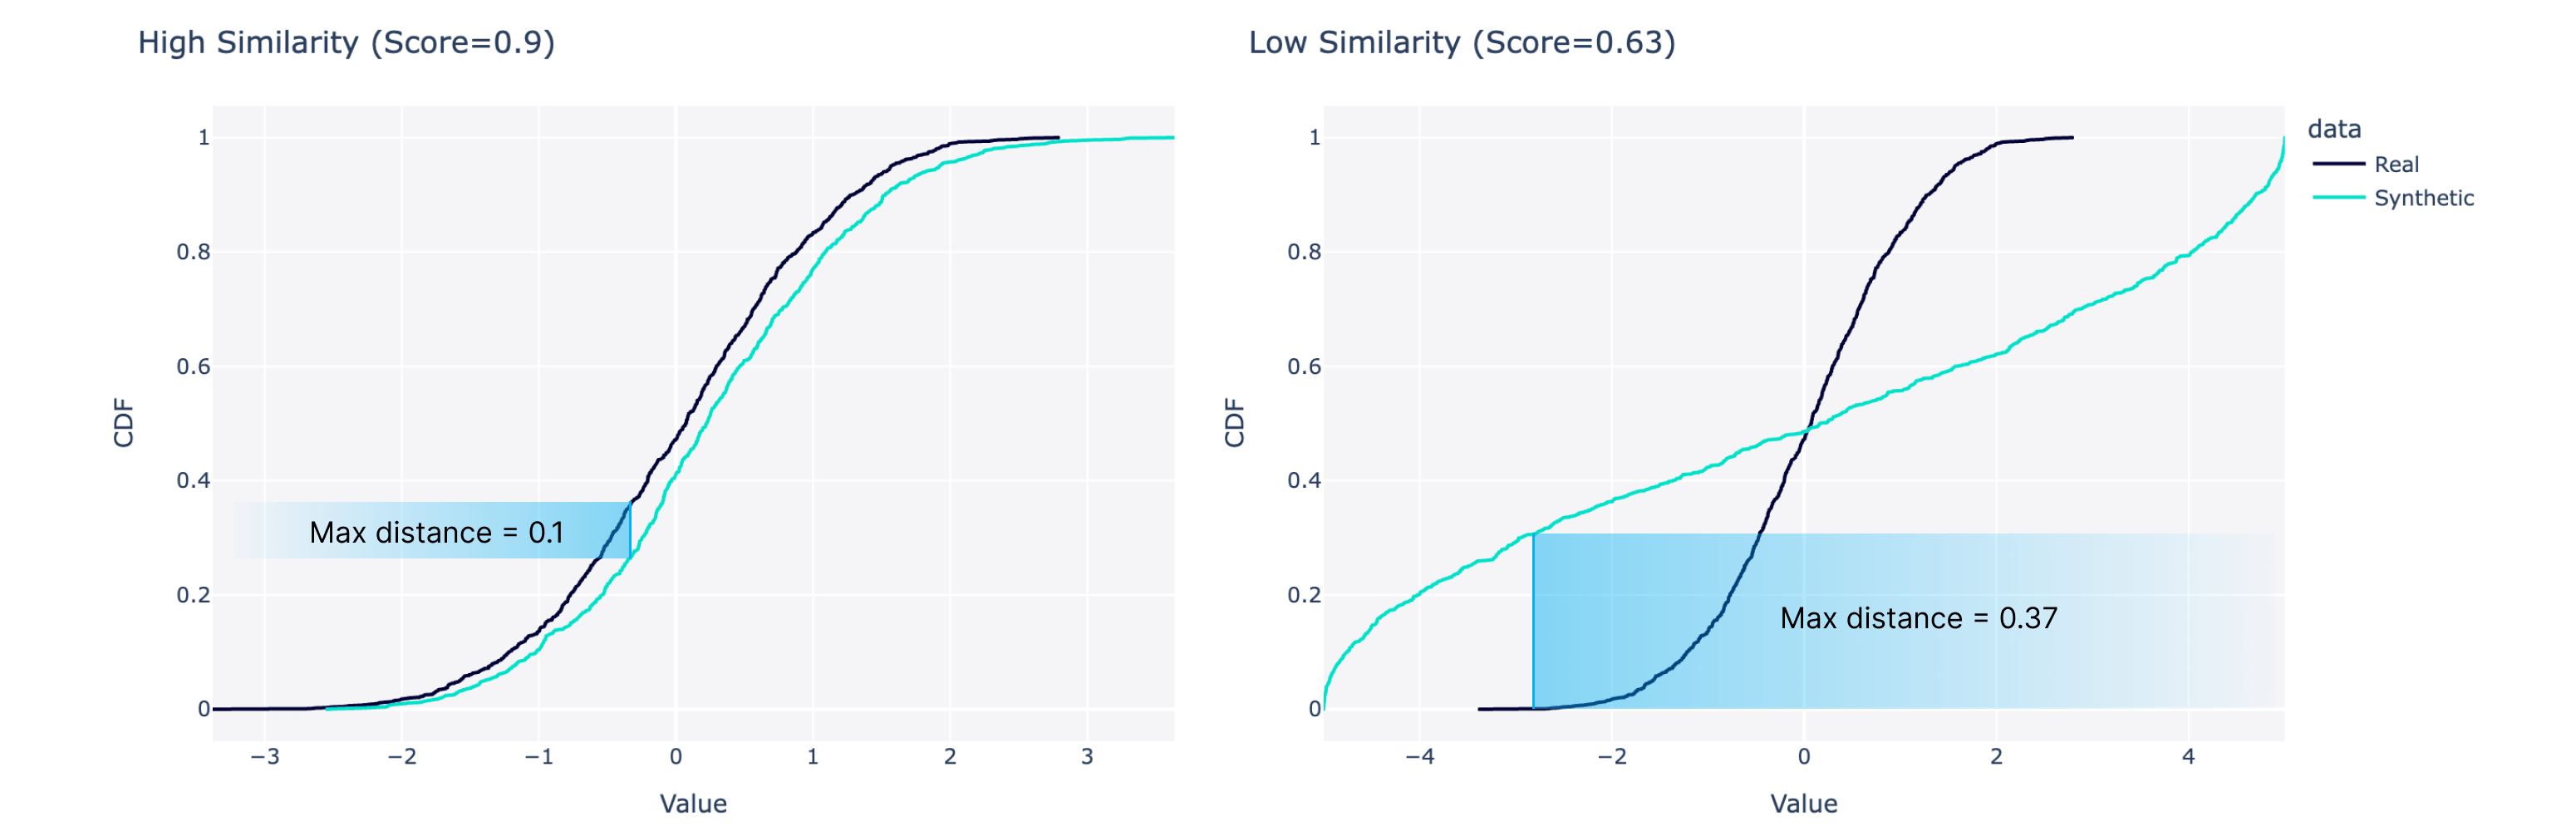
\includegraphics[width=.7\textwidth]{imagenes/SDMetrics/KSComplement_Description.png} 
    \caption{Ejemplo de SDMetric en calculo de CDF \cite{noauthor_synthetic_nodate}}
    \label{sdmetric_cdf} % puedes referirte a la imagen en tu documento usando \ref{fig:my_label}
\end{figure}

\emph{TVComplement} calcula la distancia de variación total, conocida como TVD por su acrónimo en inglés de \emph{Total Variation Distance}, entre las columnas reales y sintéticas. Para lograr esto, en primer lugar estima la frecuencia de cada valor de categoría y la expresa en términos de probabilidad. La estadística TVD compara las diferencias en estas probabilidades, siguiendo la fórmula:
\[
\delta(R,S) = 2 \sum_{\omega \in \Omega} |R_\omega - S_\omega|
\]
Aquí, $\omega$ representa todas las posibles categorías en una columna, $\Omega$. Por otro lado, $R$ y $S$ hacen referencia a las frecuencias reales y sintéticas para dichas categorías, respectivamente. \emph{TVComplement} retorna $1 - \text{TVD}$ de modo que una puntuación más alta denote una calidad superior.


El segundo componente, \emph{Column Pair Trends}, evalúa la capacidad de los datos sintéticos para replicar las correlaciones y tendencias entre cada par de columnas en los datos reales. Esta métrica se basa en la forma de las columnas individuales, las correlaciones entre cada par de columnas y la cardinalidad entre las tablas. Utiliza la métrica \emph{CorrelationSimilarity} para medir la correlación entre pares de columnas numéricas y calcular la similitud entre los datos reales y sintéticos. La métrica \emph{CorrelationSimilarity} soporta tanto los coeficientes de correlación de Pearson como de Spearman, proporcionando una evaluación flexible de las relaciones entre los datos.


\emph{CorrelationSimilarity} es una métrica únicamente aplicable a variables numéricas; las fechas son transformadas a números para este fin. Esta métrica calcula la correlación utilizando los coeficientes de Pearson y Spearman. El score se obtiene mediante la siguiente fórmula, donde $S_{A,B}$ representa la correlación del conjunto sintético y $R_{A,B}$ la correlación del conjunto real.
\[
score = 1 - \frac{|S_{A,B} - R_{A.B}|}{2}
\]


\subsection{Correlación}
En esta sección, se emplea la métrica de correlación de Pearson en las columnas numéricas, transformando las fechas en números e ignorando los valores ausentes, con el propósito de generar una representación visual en un mapa de calor para su análisis.


\subsection{Privacidad}
La Distancia al Registro más Cercano (DCR, por sus siglas en inglés) se emplea para cuantificar la distancia euclidiana entre cualquier registro sintético y su vecino real más próximo. Idealmente, a medida que la DCR se incrementa, el riesgo de violación de la privacidad disminuye. Adicionalmente, se estima el percentil 5 de esta métrica para proporcionar una medición robusta del riesgo de privacidad \cite{zhao_ctab-gan_2021}.

Relación de Distancia del Vecino más Cercano (NNDR, por sus siglas en inglés). La NNDR mide la relación entre la distancia euclidiana para el vecino real más cercano y el segundo vecino real más cercano a cualquier registro sintético correspondiente. NNDR es un concepto comúnmente utilizado en el área de visión por computadora para el emparejamiento de descriptores de imagen locales. Platzer \cite{noauthor_virtual_2022} introduce esta idea para evaluar la privacidad de los datos sintéticos. Esta relación está dentro del intervalo [0, 1]. Valores más altos indican una mejor privacidad. Los valores bajos de NNDR entre datos sintéticos y reales pueden revelar información sensible del registro de datos reales más cercano. La Fig. 6 ilustra el caso. Tenga en cuenta que también se calcula aquí el percentil 5 \cite{zhao_ctab-gan_2021}.

\subsection{Propiedades estadísticas y tecnicas de análisis}

\begin{longtable}{|m{7em}|m{5em}|m{20em}|}
    \caption{Listado de conjunto estadísticos} 
    \label{tab-stats} \\
    \hline
    \rowcolor[gray]{0.8}
    Nombre & abrev. & Descripción \\
    \hline
    \endfirsthead
    
    \hline
    \rowcolor[gray]{0.8}
    Nombre & abrev. & Descripción \\
    \hline
    \endhead
    
    \hline \multicolumn{2}{|r|}{{Continúa en la siguiente página}} \\ \hline
    \endfoot
    
    \hline \hline
    \endlastfoot
    \hline
    Numero de observaciones & nobs & Cuenta de elementos \\
    \hline
    Vacios & missing & Numero de elementos vacios \\
    \hline
    Media & mean & La suma de todos los valores dividido por el número total de valores \\
    \hline
    Mediana & median & El valor que se encuentra en el centro de un conjunto de datos ordenados de menor a mayor. Es decir, la mitad de los valores son mayores que la mediana y la otra mitad son menores \\
    \hline
    Moda & mode & El valor que aparece con mayor frecuencia en un conjunto de datos \\
    \hline
    Mínimo & min & El valor más pequeño en un conjunto de datos \\
    \hline
    Máximo & max & El valor más grande en un conjunto de datos \\
    \hline
    Percentil & 0.1\%, ... 99.9\% & El valor tal que P (25 o 75) por ciento de los datos son menores que él, y el restante (100 - P) por ciento son mayores. Cuando P = 50, el percentil es la mediana \\
    \hline
    Media Truncada & tmean & El promedio de todos los valores, una vez que se han eliminado un porcentaje de los valores más bajos y un porcentaje de los valores más altos \\
    \hline
    Varianza & var & La medida de cuán dispersos están los valores en un conjunto de datos. Es la suma de los cuadrados de las desviaciones desde la media dividido por n - 1, donde n es el número de valores \\
    \hline
    Desviación Estándar & std & La raíz cuadrada de la varianza \\
    \hline
    Error estándar de la media & std\_err & Medida de la variación de las muestras de la media poblacional. \\
    \hline
    Desviación Absoluta Media & mad & La media de los valores absolutos de las desviaciones desde la media \\
    \hline
    Desviación Mediana Absoluta Normalizada & mad\_normal & Medida de dispersión basada en la mediana que normaliza la desviación mediana absoluta utilizando la constante de escala 1.4826 para la distribución normal. \\
    \hline
    Rango & range & La diferencia entre el valor más grande y el valor más pequeño en un conjunto de datos \\
    \hline
    Tablas de Frecuencia & top5\_freq & Un método para resumir los datos al contar cuántas veces ocurre cada valor en un conjunto de datos \\
    \hline
    Probabilidad & top5\_prob & La medida de la posibilidad de que un evento ocurra. Se establece como el número de ocurrencias de un valor dividido por el número total de ocurrencias \\
    \hline
    Tabla de Contingencia & cont\_table & Una tabla que muestra la distribución conjunta de dos o más variables categóricas \\
    \hline
    Comparación de Modelos Predictivos Multivariables & cross\_pred & Un método para comparar varios modelos predictivos que involucran múltiples variables. Implica la construcción de modelos separados para cada variable objetivo y comparar la curva ROC (Receiver Operating Characteristic) para cada modelo \\
    \hline
    Kullback-Leibler & kl & Una medida de la divergencia entre dos distribuciones de probabilidad \\
    \hline
    Log-Cluster & log\_cluster & Un método para evaluar la calidad de los conjuntos de datos sintéticos que compara la estructura de los conjuntos de datos reales y sintéticos mediante el uso de clustering \\
    \hline
    Cross-Classification & cross\_class & Un método para evaluar la calidad de los conjuntos de datos sintéticos que compara la precisión de los modelos predictivos construidos a partir de los conjuntos de datos reales y sintéticos \\
    \hline
    Intervalo de confianza superior & upper\_ci & Valor máximo del intervalo de confianza alrededor de la media. \\
    \hline
    Intervalo de confianza inferior & lower\_ci & Valor mínimo del intervalo de confianza alrededor de la media. \\
    \hline
    Rango intercuartil & iqr & Diferencia entre el tercer y el primer cuartil, mide la dispersión de los datos. \\
    \hline
    Rango intercuartil normalizado & iqr\_normal & Rango intercuartil dividido por la media, para normalizar los valores. \\
    \hline
    Coeficiente de variación & coef\_var & Relación entre la desviación estándar y la media, mide la dispersión relativa de los datos. \\
    \hline
    Sesgo & skew & Medida de la asimetría de la distribución de los datos alrededor de la media. \\
    \hline
    Curtosis & kurtosis & Medida de la "pesadez" de las colas de la distribución de los datos. \\
    \hline
    Test de Jarque-Bera & jarque\_bera & Estadístico que mide si los datos tienen la asimetría y la curtosis correspondiente a una distribución normal. \\
    \hline
    p-valor del test de Jarque-Bera & jarque\_bera \_pval & Probabilidad de que los datos sean normalmente distribuidos según el test de Jarque-Bera. \\
    \hline

\end{longtable}

\chapter{Desarrollo}
\label{chap:desarrollo}
La generación de datos sintéticos es una práctica en rápida evolución con implicaciones significativas para el campo de la inteligencia artificial. Este capítulo se centra en proporcionar una visión detallada del desarrollo y la implementación este proceso, con el fin de la generación de dichos datos.

En primer lugar, se examinan los recursos disponibles que forman la base de este estudio. Se describen dos conjuntos de datos principales: uno derivado de la información de los precios de las viviendas de King County y otro de Economicos.cl, un portal chileno de anuncios clasificados. Además, se proporciona información detallada sobre el equipo informático y el software empleado en este estudio.

El núcleo de este capítulo se centra en la explicación del desarrollo de un proceso de generación de datos sintéticos. Este proceso se basa en la metodología propuesta por Synthetic Data Vault (SDV) y se extiende para incluir etapas intermedias de almacenamiento de modelos y resultados de evaluación. Se proporciona una descripción detallada de cada paso del proceso, desde la creación de metadatos hasta la generación del conjunto de datos sintéticos.

Para concluir, se abordan los métodos para la evaluación de los conjuntos de datos sintéticos generados. Esto incluye la descripción de cómo se obtienen y calculan las métricas, con un ejemplo de cómo calcular y visualizar el score promedio para una selección específica de modelos. Este capítulo prepara el terreno para un análisis profundo de los resultados obtenidos a través de esta metodología, que se presentará en los capítulos siguientes.

\section{Recursos disponibles}
\label{sec:recursos}
\subsection{Conjuntos de datos}
\label{subsec:datos}
A continuación se describen y detallan las bases de datos utilizadas en los experimentos.

\subsubsection{King County}
La base de datos de King County \cite{kaggle_house_2015} contiene notificación sobre precios de venta y características de 21,613 viviendas en Seattle y King County de los años 2014 y 2015. La base incluye datos como el número de habitaciones, el número de baños, la superficie del terreno y la superficie construida, así como detalles sobre la ubicación de la propiedad, como la latitud y la longitud. Este paquete de datos es comúnmente utilizado para tareas de regresión y predicción de precios de viviendas. Sus campos se describen en la Tabla \ref{data-county}.
 
\begin{table}[H]
	\centering
	\caption{Conjunto de datos King County}
	\label{data-county}
    \begin{tabular}{|l|m{30em}|}
        \hline
        \rowcolor[gray]{0.8}
        Variable & Descripción \\
        \hline
        id & Identificación \\
        \hline
        date & Fecha de venta \\
        \hline
        price & Precio de venta \\
        \hline
        bedrooms & Número de dormitorios \\
        \hline
        bathrooms & Número de baños \\
        \hline
        sqft\_liv & Tamaño del área habitable en pies cuadrados \\
        \hline
        sqft\_lot & Tamaño del terreno en pies cuadrados \\
        \hline
        floors & Número de pisos \\
        \hline
        waterfront & '1' si la propiedad tiene vista al mar, '0' si no \\
        \hline
        view & Índice del 0 al 4 de la calidad de la vista de la propiedad \\
        \hline
        condition & Condición de la casa, clasificada del 1 al 5 \\
        \hline
        grade & Clasificación por calidad de construcción que se refiere a los tipos de materiales utilizados y la calidad de la mano de obra. Los edificios de mejor calidad (grado más alto) cuestan más construir por unidad de medida y tienen un valor más alto. Información adicional en: KingCounty \\
        \hline
        sqft\_above & Pies cuadrados sobre el nivel del suelo \\
        \hline
        sqft\_basmt & Pies cuadrados debajo del nivel del suelo \\
        \hline
        yr\_built & Año de construcción \\
        \hline
        yr\_renov & Año de renovación. '0' si nunca se ha renovado \\
        \hline
        zipcode & Código postal de 5 dígitos \\
        \hline
        lat & Latitud \\
        \hline
        long & Longitud \\
        \hline
        sqft\_liv15 & Tamaño promedio del espacio habitable interior para las 15 casas más cercanas, en pies cuadrados \\
        \hline
        sqft\_lot15 & Tamaño promedio de los terrenos para las 15 casas más cercanas, en pies cuadrados \\
        \hline
        Shape\_leng & Longitud del polígono en metros \\
        \hline
        Shape\_Area & Área del polígono en metros \\
        \hline
    \end{tabular}
\end{table}  


\subsubsection{Economicos}
Economicos.cl es un portal web chileno que se especializa en la publicación de anuncios clasificados en línea, enfocándose en las categorías de bienes raíces, vehículos, empleos, servicios y productos variados. 
La base de datos se originó de un \emph{Web Scraping} ejecutado en 2020, y contiene 22.059 observaciones.

\begin{table}[H]
	\centering
	\caption{Base de datos Economicos.cl}
	\label{data-economicos}
    \begin{tabular}{|l|m{30em}|}
        \hline
        \rowcolor[gray]{0.8}
        Variable & Descripción \\
        \hline
        url & URL de la publicación \\
        \hline
        Descripción & Detalles de la publicación \\
        \hline
        price & Valor de venta, en dólares, UF o pesos \\
        \hline
        property\_type & Clase de propiedad: Casa, Departamento, etc. \\
        \hline
        transaction\_type & Clase de transacción\: Arriendo, Venta \\
        \hline
        state & Región de la publicación \\
        \hline
        county & Comuna de la publicación \\
        \hline
        publication\_date & Fecha de la publicación \\
        \hline
        rooms & Cantidad de dormitorios \\
        \hline
        bathrooms & Cantidad de baños \\
        \hline
        m\_built & Extensión del área habitable en metros cuadrados \\
        \hline
        m\_size & Extensión del terreno en metros cuadrados \\
        \hline
        source & Medio de la publicación \\
        \hline
        title & Título de la publicación \\
        \hline
        address & Dirección de la publicación \\
        \hline
        owner & Publicador \\
        \hline
        \_price & Valor convertido a UF del día de la publicación \\
        \hline
    \end{tabular}
\end{table}




\subsection{Computación y Software}
\label{subsec:computacion}
Para efectuar los experimentos, se recurrió a un equipo informático con las especificaciones técnicas detalladas en la Tabla \ref{tabla-componentes-pc}. El procesador seleccionado fue un AMD Ryzen 9 7950X 16-Core Procesadores, complementado con cuatro módulos de 32 GB para sumar una memoria total de 128 GB DDR5. La tarjeta gráfica incorporada fue una NVIDIA GeForce RTX 4090, y el equipo contó con dos discos duros de 500 GB SSD. El uso de un sistema con estas características garantizó una ejecución eficaz de los modelos de generación de datos, asegurando la viabilidad de los experimentos. Cabe resaltar que la selección de los componentes del equipo se realizó de manera meticulosa para garantizar que los resultados obtenidos no se vieran afectados por una capacidad de hardware limitada.

En lo que respecta al software, se empleó el sistema operativo Ubuntu 20.04.2 LTS y se utilizó el lenguaje de programación Python 3.10 para la implementación de los modelos de generación de datos. Se recurrió a diversas bibliotecas, incluyendo DVC, SDV y PyTorch, cuya lista completa está disponible en el \href{https://github.com/gvillarroel/synthetic-data-for-text/blob/main/freeze.txt}{repositorio en Github}. La elección de estas herramientas estuvo guiada por su compatibilidad con el modelo TabDDPM, el cual fue empleado en algunos de los experimentos.


\begin{table}[H]
	\centering
	\caption{Computador Usado}
	\label{tabla-componentes-pc}
    \begin{tabular}{|l|l|}
        \hline
        \rowcolor[gray]{0.8}
        Componente & Descripción \\
        \hline
        Procesador & AMD Ryzen 9 7950X 16-Core Processor \\
        \hline
        Memoria RAM & 128 GB DDR5 \\
        \hline
        Tarjeta gráfica & NVIDIA GeForce RTX 4090 \\
        \hline
        Disco duro & 1 TB SSD \\
        \hline
      \end{tabular}        
\end{table}  

Con el objetivo de asegurar la reproducibilidad, se implementó \textit{devcontainer}, que configura el entorno de desarrollo y pruebas mediante una imagen replicable de \textit{Docker}. Los experimentos pueden ser reproducidos utilizando el contenedor descrito en el repositorio y el Código \ref{devcontainer-file}.

\begin{listing}[H]
\inputminted[
    framesep=5pt, rulecolor=gray,
    fontsize=\small,
    linenos=true, 
    breaklines=true,xleftmargin=1.0cm
    ]{json}{../../.devcontainer/devcontainer.json}
\caption{Devcontainer del proyecto en curso.}
\label{devcontainer-file}
\end{listing}


El código fuente de los modelos destinados a la generación de datos, así como los scripts para el análisis y la representación gráfica de los resultados, se encuentran disponibles en un repositorio público de Github:
\href{https://github.com/gvillarroel/synthetic-data-for-text}{gvillarroel/synthetic-data-for-text}. Se requiere el uso de DVC para la descarga de datos desde un directorio compartido en Google Drive.

\newpage

\section{Desarrollo del flujo de procesamiento}
\label{subsec:procesamiento}
En las siguientes secciones se detalla el flujo de procesamiento implementado para la generación de nuevos datos sintéticos. Este flujo se inspira en el propuesto por Synthetic Data Vault (SDV), incorporando algunas modificaciones para preservar etapas intermedias.

SDV es un ecosistema de bibliotecas para la generación de datos sintéticos que facilita a los usuarios aprender de bases de datos unidimensionales, multidimensionales y de series temporales, para posteriormente generar nuevos datos sintéticos que mantengan las mismas propiedades estadísticas y el mismo formato que las bases de datos originales. Para conseguir esto, SDV emplea diversas técnicas, como modelos generativos y redes neuronales, con el fin de aprender la distribución subyacente de los datos y generar nuevos datos que sigan dicha distribición \cite{kotelnikov_overview_nodate, patki_synthetic_2016}.

A continuación, se explica el proceso de generación de datos sintéticos para una base de datos unidimensional utilizando la biblioteca Synthetic Data Vault (SDV), seguido de las modificaciones introducidas para expandir el proceso e incorporar nuevos modelos.

En la Tabla \ref{process-sdv} se muestran los pasos necesarios para generar un conjunto de datos sintéticos utilizando SDV:

\begin{figure}[H]
	\centering
	\includesvg[scale=.2,inkscapelatex=false]{../dfd/images/processor.svg}
	\caption{Proceso para generar datos sintéticos con SDV}
	\label{process-sdv}
\end{figure}

\begin{enumerate}
    \item \textbf{Creación de Metadatos}: Se elabora un diccionario que define los campos del conjunto de datos y los tipos de datos que contiene. Esto le permite a SDV aprender la estructura del conjunto de datos original y utilizarla para generar nuevos datos sintéticos con la misma estructura.
    \item \textbf{Creación del Modelo}: Se selecciona el modelo de generación de datos a utilizar. SDV proporciona varios modelos, entre ellos GaussianCopula, CTGAN, CopulaGAN y TVAE, que se adaptan a distintos tipos de datos y distribuciones.
    \item \textbf{Entrenamiento del Modelo}: El modelo seleccionado se entrena con el conjunto de datos original para aprender sus distribuciones y patrones estadísticos.
    \item \textbf{Generación del Conjunto de Datos Sintéticos}: Con el modelo ya entrenado, se generan nuevos datos sintéticos que mantienen la misma estructura y características estadísticas que el conjunto original. Este nuevo conjunto de datos puede ser empleado para diversas aplicaciones, como pruebas de software o análisis de datos sensibles.
\end{enumerate}
Es crucial señalar que el proceso de generación de datos sintéticos con SDV es escalable y puede aplicarse a bases de datos unidimensionales, multidimensionales y de series temporales. Adicionalmente, en este proyecto se introdujeron ciertas modificaciones al flujo para expandir el proceso y facilitar la incorporación de nuevos modelos.
\newpage
En el proceso extendido de generación de datos sintéticos con SDV, se introducen dos nuevas etapas para permitir el almacenamiento de los modelos intermedios y los resultados de la evaluación. El proceso completo se ilustra en la Figura \ref{process-sdv-2} y comprende los siguientes pasos:


\begin{enumerate}
    \item \textbf{Creación de Metadatos}: Se elabora un diccionario que define los campos del conjunto de datos y los tipos de datos que contiene.
    \item \textbf{Creación del Modelo}: Se selecciona el modelo a utilizar. SDV permite elegir entre GaussianCopula, CTGAN, CopulaGAN y TVAE.
    \item \textbf{Entrenamiento del Modelo}: El modelo seleccionado se entrena con el conjunto de datos original para aprender sus distribuciones.
    \item \textbf{Guardado del Modelo}: El modelo entrenado se almacena en un archivo para su uso posterior.
    \item \textbf{Generación del Conjunto de Datos Sintéticos}: Se genera un nuevo conjunto de datos utilizando el modelo entrenado.
    \item \textbf{Evaluación y Guardado de Métricas}: Se evalúa el conjunto de datos sintético generado y se almacenan las métricas, como la correlación, el error absoluto medio y el error cuadrático medio.
\end{enumerate}


\begin{figure}[H]
	\centering
	\includesvg[scale=.15,inkscapelatex=false]{../dfd/images/processor_edited.svg}
	\caption{Proceso para generar datos sintéticos completo}
	\label{process-sdv-2}
\end{figure}

Con estas nuevas etapas, se pueden guardar los modelos intermedios y los resultados de la evaluación, lo que permite una mayor flexibilidad en el proceso y la capacidad de utilizar los modelos y los resultados en posteriores experimentos.



\section{Modelos de generación de datos}
\label{subsec:generacion}

Los modelos de generación de datos tabulares se fundamentan en la metodología propuesta por \emph{Synthetic Data Vault} (SDV), mientras que los modelos de generación de texto utilizan la biblioteca Hugging Face para cargar, realizar \emph{fine-tuning} con nuevas tareas y evaluar el modelo basado en mT5.

\subsection{Modelos para datos tabulares}
Para que un modelo sea compatible con SDV, debe implementar los siguientes métodos:
\begin{enumerate}
    \item \textbf{cargar} (load): Carga el modelo desde un archivo.
    \item \textbf{entrenar} (fit): Entrena el modelo, tomando como entrada un dataframe de pandas.
    \item \textbf{guardar} (save): Almacena el modelo en un archivo.
    \item \textbf{muestrear} (sample): Genera un conjunto de nuevos registros utilizando el modelo entrenado.
\end{enumerate}


Como consideración adicional, se aconseja llevar a cabo el proceso mediante un script en lugar de un cuaderno Jupyter, dado que se ha observado que el cuaderno puede encontrar problemas con algunos modelos debido a restricciones de memoria. A continuación, se especifican los pasos para la ejecución del proceso:
\begin{enumerate}
\item Generar un archivo de configuración que contenga la información requerida para la generación de datos sintéticos, como la ruta del conjunto de datos original y la configuración de los modelos a emplear.
\item Crear un script que cargue la configuración, ejecute el proceso de generación de datos sintéticos y almacene el conjunto de datos sintético resultante.
\item Poner en marcha el script creado en el paso previo.
\end{enumerate}


De esta forma, es posible automatizar el proceso de generación de datos sintéticos y aprovechar una mayor capacidad de procesamiento, lo que puede mejorar el rendimiento del proceso y reducir los tiempos de ejecución.

La clase \emph{Synthetic} es una implementación que permite configurar los modelos a utilizar en el proceso de generación de datos sintéticos. Esta clase encapsula los métodos comunes de los modelos, como \emph{load}, \emph{fit}, \emph{save} y \emph{sample}, lo que permite una configuración general de las entradas y la selección de modelos.


En el ejemplo presentado en el Código \ref{code-economicos-synthetic}, se crea una instancia de la clase \emph{Synthetic} utilizando un pandas dataframe previamente preprocesado. Se especifican las columnas que se considerarán como categorías, las que se considerarán como texto y las que se excluirán del análisis. Además, se indica el directorio donde se almacenarán los archivos temporales, se seleccionan los modelos a utilizar, se establece el número de registros sintéticos deseados y se define una columna objetivo para realizar pruebas con aprendizaje automático y estratificar los conjuntos parciales de datos que se utilizarán. De esta manera, se configura de forma flexible el proceso de generación de datos sintéticos según las necesidades específicas del usuario.

\begin{listing}[H]
\inputminted[
    firstline=45, lastline=54
    ]{python}{../../notebooks/economicos_train.py}
\caption{Instanciando clase Synthetic}
\label{code-economicos-synthetic}
\end{listing}

La Tabla \ref{synthetic-input} presenta las opciones para la instancia de la clase \emph{Synthetic}:

\begin{table}[H]
\centering
\caption{Variables de entrada para \emph{Synthetic}}
\label{synthetic-input}
\begin{tabular}{|l|m{25em}|}
\hline
\rowcolor[gray]{0.8}
\textbf{Variable} & \textbf{Descripción} \\
\hline
df & Pandas DataFrame a utilizar \\
\hline
Id & Nombre de la columna a ser usada como identificadora \\
\hline
category\_columns & Listado de columnas categóricas \\
\hline
text\_columns & Listado de columnas de texto \\
\hline
exclude\_columns & Listado de columnas que deben ser excluidas \\
\hline
synthetic\_folder & Carpeta donde se guardarán los documentos intermedios y finales \\
\hline
models & Listado de modelos a utilizar \\
\hline
n\_sample & Número de registros a generar \\
\hline
target\_column & Columna a utilizar como objetivo para modelos de machine learning en las evaluaciones y separación cuando se deba estratificar los campos. \\
\hline
\end{tabular}
\end{table}

En la Tabla \ref{modelos-tab-soportados} se detallan los modelos actualmente soportados en la clase \emph{Synthetic} y su origen.

\begin{table}[H]
	\centering
	\caption{Modelos Tabulares Soportados}
	\label{modelos-tab-soportados}
    \begin{tabular}{|l|l|}
        \hline
        \rowcolor[gray]{0.8}
        Nombre Modelo & Fuente \\
        \hline
        copulagan & SDV \cite{kotelnikov_overview_nodate} \\
        \hline
        tvae & SDV \cite{kotelnikov_overview_nodate} \\
        \hline
        gaussiancopula & SDV \cite{kotelnikov_overview_nodate} \\
        \hline
        ctgan & SDV \cite{kotelnikov_overview_nodate} \\
        \hline
        tablepreset & SDV \cite{kotelnikov_overview_nodate} \\
        \hline
        smote-enc & tabDDPM \cite{akim_tabddpm_2023} \\
        \hline
        tddpm\_mlp & tabDDPM \cite{akim_tabddpm_2023} \\
        \hline
      \end{tabular}        
\end{table} 

Al ejecutar el script de generación de datos sintéticos, se crearán múltiples archivos en una carpeta. En la Tabla \ref{synth-folders} se muestra un ejemplo de los archivos generados y su formato. El nombre del modelo utilizado se indica en el campo \textbf{<model>}, y en caso de haberse aplicado \emph{Differential Privacy} para generar una versión con ruido. El campo \textbf{<n\_sample>} indica el número de registros sintéticos generados, y finalmente el campo \textbf{<type\_comparison>} especifica si se trata de una comparación entre los datos sintéticos y los datos de entrenamiento (\emph{Synthetic vs Train}, abreviado como ST) o entre los datos sintéticos y los datos de validación (\emph{Synthetic vs Hold}, abreviado como SH). Adicionalmente se encuentran los archivos de esquema (\emph{metadata.json}) y una separación del dataset inicial en el conjunto de entrenamiento y test (hold).
\begin{figure}[H]
	\centering
	\includesvg[scale=1,inkscapelatex=false]{../dfd/images/synth_tree.svg}
	\caption{Carpetas y archivos esperados generados por \emph{Synthetic}}
	\label{synth-folders}
\end{figure}


\newpage
\subsection{Modelos para textos}
Como se mencionó anteriormente, se utilizó el modelo \textbf{mT5} que se entrenó para una nueva tarea utilizando la estrategia presentada en el artículo \emph{Text-to-Text Pre-Training for Data-to-Text Tasks} \cite{kale_text--text_2020}. Para ilustrar el proceso, se presenta un ejemplo del texto pre-procesado, el segmento de la pregunta y la respuesta esperada para un registro del conjunto de datos \emph{economicos.cl}.

\begin{tcolorbox}[colback=white,colframe=black!50!white,title=Input]
<fecha, 2022-01-01>\\
<precio, \$ 105.000.000>\\
<tipo, Departamento>\\
<transacci\'on, Venta>\\
<regi\'on, Metropolitana de Santiago>\\
<comuna, Santiago>\\
<dormitorios, 3.0>\\
<ba\~nos, 3.0>\\
<construidos, 47.0>\\
<terreno, 47.0>\\
<precio\_real, 3387.4540447373292>\\
<titulo, Departamento en Venta en Santiago 3 dormitorios 1 ba\~no>\\
<direcci\'on, DEPARTAMENTO EN EL CORAZON DE LO BARNECHEA Santiago, Metropolitana de Santiago>
\end{tcolorbox}
\begin{tcolorbox}[colback=white,colframe=black!50!white,title=Tarea]
descripci\'on de esta publicaci\'on
\end{tcolorbox}
\begin{tcolorbox}[colback=white,colframe=black!50!white,title=Respuesta esperada]
\footnotesize
Kazona Propiedades Vende Departamento de 47m2, 3 dormitorios, 1 ba\~no, cocina, living comedor , Paredes con Cer\'amica y Tabiquer\'ia en techo con madera barnizada timbrada, ventanas nuevas de PVC y vidrio termolaminado, sistema el\'ectrico actualizado, departamento ubicado en el 3er nivel (sin ascensor) , bajo gasto com\'un. Excelentes conectividades y ubicaci\'on en Pleno Centro De Lo Barnechea, como colegios privados y p\'ublicos, supermercados, Mall Portal La Dehesa, locomoci\'on, entre otros.\\
Podemos destacar de la propiedad:\\
Pleno Centro Lo Barnechea\\
100 metros de locomoci\'on a Escuela Militar , Bilbao, Stgo Centro, Mapocho\\
200 metros colegios Montessori Nido de \'Aguila, San Rafael , otros\\
200 metros Mall Portal La Dehesa\\
200 metros Sta. Isabel\\
300 metros carabineros\\
Gastos comunes bajos  \$10.000\\
Estacionamiento comunitario\\
No paga contribuciones\\
Contactanos al telefono Kazona 569 56031154
\end{tcolorbox}

\section{Obtención de Métricas}
\label{subsec:metricas}

Se han automatizado la mayoría de las métricas para evaluar los conjuntos de datos sintéticos mediante el módulo \emph{metrics}. Estas métricas se aplican a los tres conjuntos de datos para su evaluación, lo que permite calcular estadísticas y comparativas para el conjunto de datos real utilizado para el entrenamiento (train dataset), el conjunto de datos reservado para la evaluación (hold) y el conjunto de datos sintético generado por los diferentes modelos (synthetic). Se pueden recolectar ejecutando el ejemplo de código proporcionado en Código \ref{code-economicos-metrics}.

\begin{listing}[H]
\inputminted[
    firstline=55, lastline=55
    ]{python}{../../notebooks/economicos_run-a.py}
\caption{Obtención de métricas en economicos\_run-a.py}
\label{code-economicos-metrics}
\end{listing}

En la Tabla \ref{metricas-numericas} se muestra las metricas recolectadas para campos numericos.

\begin{longtable}{|m{10em}|m{25em}|}
    \caption{Metricas para campos numericos} 
    \label{metricas-numericas} \\
    \hline
    \rowcolor[gray]{0.8}
    Campo & Ejemplos \\
    \hline
    \endfirsthead
    
    \hline
    \rowcolor[gray]{0.8}
    Campo & Ejemplos \\
    \hline
    \endhead
    
    \hline \multicolumn{2}{|r|}{{Continúa en la siguiente página}} \\ \hline
    \endfoot
    
    \hline \hline
    \endlastfoot
    
    \hline
    Nombre del campo (name) & sqft\_living \\ \hline
    Valores del Top 5 (top5) & [1400 1300 1720 1250 1540] \\ \hline
    Frecuencia Top 5 (top5\_frec) & [109 107 106 106 105] \\ \hline
    Probabilidades de Top 5 (top5\_prob) & [0.00630422 0.00618855 0.00613071 0.00613071 0.00607287] \\ \hline
    Elementos observados (nobs) & 17290 \\ \hline
    Nulos (missing) & 0 \\ \hline
    Promedio (mean) & 2073.894910 \\ \hline
    Desviación Estándar (std) & 907.297963 \\ \hline
    Error estándar de la media (std\_err) & 6.900053 \\ \hline
    Intervalo de confianza superior (upper\_ci) & 2087.418766 \\ \hline
    Intervalo de confianza inferior (lower\_ci) & 2060.371055 \\ \hline
    Rango intercuartílico (iqr) & 1110 \\ \hline
    Rango intercuartílico normalizado (iqr\_normal) & 822.844231 \\ \hline
    Desviación absoluta de la mediana (mad) & 693.180169 \\ \hline
    Desviación absoluta de la mediana normalizada (mad\_normal) & 868.772506 \\ \hline
    Coeficiente de variación (coef\_var) & 0.437485 \\ \hline
    Rango (range) & 11760 \\ \hline
    Valor máximo (max) & 12050 \\ \hline
    Valor mínimo (min) & 290 \\ \hline
    Sesgo (skew) & 1.370859 \\ \hline
    Curtosis (kurtosis) & 7.166622 \\ \hline
    Test de normalidad de Jarque-Bera (jarque\_bera) & 17922.347382 \\ \hline
    Valor p del test de normalidad de Jarque-Bera (jarque\_bera\_pval) & 0 \\ \hline
    Moda (mode) & 1400 \\ \hline
    Frecuencia de la moda (mode\_freq) & 0.006304 \\ \hline
    Mediana (median) & 1910 \\ \hline
    Percentil 0.1\% & 522.890000 \\ \hline
    Percentil 1\% & 720 \\ \hline
    Percentil 5\% & 940 \\ \hline
    Percentil 25\% & 1430 \\ \hline
    Percentil 75\% & 2540 \\ \hline
    Percentil 95\% & 3740 \\ \hline
    Percentil 99\% & 4921.100000 \\ \hline
    Percentil 99.9\% & 6965.550000 \\ \hline
\end{longtable}

En la Tabla \ref{metricas-categoricas} se muestran los datos calculados para campos categóricos.

\begin{table}[H]
    \centering
    \caption{Métricas para campos categóricos}
    \label{metricas-categoricas}
    \begin{tabular}{|m{10em}|m{25em}|}
        \hline
        \rowcolor[gray]{0.8}
        Nombre del campo (name) & waterfront \\ \hline
        Valores del Top 5 (top5) & [0 1] \\ \hline
        Frecuencia Top 5 (top5\_freq) & [17166   124] \\ \hline
        Probabilidades de Top 5 (top5\_prob) & [0.99282822 0.00717178] \\ \hline
        Elementos observados (nobs) & 17290.0 \\ \hline
        Nulos (missing) & 17290.0 \\ \hline
    \end{tabular}
\end{table}

En el Código \ref{codigo-show-score}, se muestra cómo se calcula y se muestra el Score promedio para una selección específica de modelos. El código utiliza la función "sort\_values" para ordenar los resultados en orden descendente según el puntaje. Luego, se filtran los resultados para incluir solo los modelos seleccionados y las columnas que muestran el puntaje y la Distancia al registro más cercano (DCR) en los tres umbrales \emph{Synthetic vs Train} (ST), \emph{Synthetic vs Hold} (SH) y \emph{Train vs Hold} TH.
\begin{listing}[H]
    \begin{minted}[linenos=true,frame=lines,framesep=2mm,baselinestretch=1.2]{python}
avg = syn.scores[syn.scores["type"] == "avg"]
avg.sort_values("score", ascending=False).loc[ ["tddpm_mlp","smote-enc","gaussiancopula","tvae","gaussiancopula", "copulagan","ctgan"], ["score", "DCR ST 5th", "DCR SH 5th", "DCR TH 5th"]]
    \end{minted}
\caption{Mostrando Scores Promedios Calculados}
\label{codigo-show-score}
\end{listing}

\chapter{Resultados}
Este proyecto se ha centrado en la generación de datos sintéticos a través de diversos métodos de preprocesamiento y modelos de aprendizaje automático. Los resultados se examinan en base al rendimiento de los modelos, los cuales fueron entrenados con los datos sintéticos, y se valoran respecto a la similitud, privacidad y utilidad de los datos generados.

Cabe mencionar que los resultados son inherentes a cada conjunto de datos y modelo utilizado. Por lo tanto, se proporciona un análisis exhaustivo de los resultados en cada escenario específico. Esto permite una mejor comprensión de la eficacia de los métodos utilizados en la generación de datos sintéticos y su comparación con los datos originales.

A continuación, se presentan los conjuntos de datos de King County y Económicos. El conjunto Económicos se subdivide en dos subconjuntos, que difieren en su tratamiento de los datos nulos durante el preprocesamiento.

\newpage
\section{King County}
\subsection{Reportes}
La Tabla \ref{table-score-king county-a} muestra los puntajes obtenidos por los distintos patrones utilizados en este estudio. Es notorio que los patrones con puntajes más altos, como tddpm\_mlp y smote-enc, presentan una mayor similitud con el conjunto de datos original. En contraposición, los patrones con puntajes más bajos, como ctgan, exhiben una correspondencia considerablemente menor con el conjunto original. Se muestra el promedio ± desviación estándar basado en las 3 ejecuciones realizadas.

\begin{table}[H]
\centering
\fontsize{9}{14}\selectfont
\caption{Evaluaci\'on de M\'etricas de Rendimiento para Diversos Modelos de Aprendizaje Autom\'atico, King County}
\label{table-score-king county-a}
\begin{tabular}{|l|r|r|r|r|r|}
\hline
\rowcolor[gray]{0.8}
Model Name & Column Pair Trends & Column Shapes & Coverage & Boundaries & \textbf{Score} \\
\hline tddpm\_mlp & 9.37e-01±3.80e-03 & \bfseries 9.67e-01±1.48e-03 & \bfseries 9.66e-01±4.96e-03 & 1.00e+00±0.00e+00 & 9.52e-01±2.36e-03 \\
\hline smote-enc & \bfseries 9.41e-01±2.60e-04 & 9.65e-01±3.06e-04 & 8.42e-01±8.31e-03 & \bfseries 1.00e+00±1.02e-05 & \bfseries 9.53e-01±2.45e-04 \\
\hline ctgan & 8.10e-01±1.40e-02 & 8.38e-01±2.67e-02 & 8.56e-01±2.25e-03 & 1.00e+00±0.00e+00 & 8.24e-01±2.02e-02 \\
\hline tablepreset & 8.37e-01±0.00e+00 & 8.37e-01±1.36e-16 & 7.53e-01±0.00e+00 & 1.00e+00±0.00e+00 & 8.37e-01±7.85e-17 \\
\hline copulagan & 7.64e-01±4.93e-03 & 8.14e-01±4.70e-03 & 8.40e-01±1.74e-02 & 1.00e+00±0.00e+00 & 7.89e-01±2.92e-03 \\
\hline gaussiancopula & 7.65e-01±0.00e+00 & 8.11e-01±0.00e+00 & 7.51e-01±7.85e-17 & 1.00e+00±0.00e+00 & 7.88e-01±0.00e+00 \\
\hline tvae & 7.07e-01±1.19e-02 & 7.68e-01±1.22e-02 & 4.53e-01±1.63e-02 & 1.00e+00±0.00e+00 & 7.38e-01±1.18e-02 \\
\hline
\end{tabular}
\end{table}
    
A pesar de que los patrones TDDPM y SMOTE alcanzan calificaciones prometedoras en general, se observa una diferencia significativa entre ambos en términos de cobertura (\emph{Coverage}). Específicamente, SMOTE no logra capturar la diversidad del conjunto de datos, reflejándose en una calificación de cobertura marcadamente inferior a la de TDDPM.

\newpage

\subsubsection{Correlación pairwise}

En el Anexo \ref{A-pairwise-kingcounty-top2-a-1}, se contrasta la lista completa de cada modelo. Se observa que, en general, los modelos con puntajes más altos exhiben una mayor similitud visual con los datos reales. A modo de ilustración, las imágenes \fullref{pairwise-king county-a-1-copulagan} y \fullref{pairwise-king county-a-1-gaussiancopula} contrastan los datos reales con los generados por los modelos gaussiancopula y copulagan. A pesar de que estos modelos presentan puntajes similares, el modelo gaussiancopula muestra una mayor similitud visual con los datos reales en comparación con el modelo copulagan.

\begin{figure}[H]
    \centering
    \includesvg[scale=.5,inkscapelatex=false]{datasets/kingcounty-a-1/pairwise/copulagan.svg}
    \caption{Correlación de conjunto Real y Modelo: copulagan}
    \label{pairwise-king county-a-1-copulagan}
\end{figure}

\begin{figure}[H]
    \centering
    \includesvg[scale=.6,inkscapelatex=false]{datasets/kingcounty-a-1/pairwise/gaussiancopula.svg}
    \caption{Correlación de conjunto original de entrenamiento y Gaussiancopula, King county (A-1)}
    \label{pairwise-king county-a-1-gaussiancopula}
\end{figure}

\newpage 
Cabe resaltar que, entre los modelos con puntajes superiores al 90\%, la evaluación visual para determinar cuál es superior puede ser un desafío. Esta dificultad surge debido a que, a medida que el puntaje se incrementa, la similitud visual entre los datos reales y los generados se intensifica. Esto se aprecia en las figuras \fullref{pairwise-king county-a-1-smote-enc} y \fullref{pairwise-king county-a-1-tddpm_mlp}, donde se contrastan los datos reales con los generados por los modelos smote-enc y tddpm\_mlp, respectivamente. Ambos modelos ostentan puntajes por encima del 90\%, y la correspondencia visual entre los datos reales y los generados es notoriamente alta en ambos casos.

\begin{figure}[H]
    \centering
    \includesvg[scale=.6,inkscapelatex=false]{datasets/kingcounty-a-1/pairwise/smote-enc.svg}
    \caption{Correlación de conjunto original de entrenamiento y Smote, King county (A-1)}
    \label{pairwise-king county-a-1-smote-enc}
\end{figure}

\begin{figure}[H]
    \centering
    \includesvg[scale=.5,inkscapelatex=false]{datasets/kingcounty-a-1/pairwise/tddpm_mlp.svg}
    \caption{Correlación de conjunto Real y Modelo: tddpm\_mlp}
    \label{pairwise-king county-a-1-tddpm_mlp}
\end{figure}
En la evaluación mediante SDMetrics y en la comparación visual a través de la correlación de Wise, los modelos más sobresalientes resultan ser TDDPM y SMOTE. Dichos modelos han logrado los puntajes más elevados en ambas métricas y han demostrado una notable similitud visual con los datos reales. Por ende, se puede inferir que estos modelos resultan ser los más eficaces para la generación de datos sintéticos beneficiosos para este conjunto de datos en particular.

\newpage
\subsubsection{Revisión de Columnas}
La Tabla \ref{table-coverage-king county-a} evidencia la predominancia del modelo TDDPM en términos de cobertura de los diferentes valores en general, aunque se presentan casos en los que ambos modelos no logran una cobertura completa. Por ejemplo, en la columna correspondientes a \emph{bedrooms}, TDDPM solo logra una cobertura que supera el 71.8\%, sin embargo, aún así supera a SMOTE. Por su parte, SMOTE solo alcanzan una cobertura del 51\% en la misma columna.


\begin{table}[H]
\centering
\fontsize{10}{14}\selectfont
\caption{Cobertura Categor{\'\i}a/Rango para Modelos Smote y Tddpm, King County}
\label{table-coverage-king county-a}
\begin{tabular}{|l|l|r|r|}
\hline
\rowcolor[gray]{0.8}
Columna & Metrica & smote-enc & tddpm\_mlp \\
\hline bathrooms & CategoryCoverage & 6.56e-01±3.85e-02 & \bfseries 8.11e-01±3.85e-02 \\
\hline bedrooms & CategoryCoverage & \cellcolor[rgb]{0.9, 0.54, 0.52} 5.13e-01±4.44e-02 & \cellcolor[rgb]{0.9, 0.54, 0.52} \bfseries 7.18e-01±4.44e-02 \\
\hline condition & CategoryCoverage & 9.33e-01±1.15e-01 & \bfseries 1.00e+00±0.00e+00 \\
\hline date & CategoryCoverage & \bfseries 9.64e-01±6.77e-03 & 9.44e-01±9.69e-03 \\
\hline floors & CategoryCoverage & 8.33e-01±0.00e+00 & \bfseries 9.44e-01±9.62e-02 \\
\hline grade & CategoryCoverage & 7.50e-01±0.00e+00 & \bfseries 8.61e-01±4.81e-02 \\
\hline id & RangeCoverage & 9.93e-01±4.54e-04 & \bfseries 1.00e+00±7.79e-04 \\
\hline lat & RangeCoverage & 9.65e-01±8.31e-03 & \bfseries 1.00e+00±0.00e+00 \\
\hline long & RangeCoverage & 9.91e-01±5.54e-03 & \bfseries 1.00e+00±2.45e-04 \\
\hline price & RangeCoverage & 5.72e-01±1.02e-01 & \bfseries 1.00e+00±1.25e-05 \\
\hline sqft\_above & RangeCoverage & 7.88e-01±2.98e-02 & \bfseries 1.00e+00±1.45e-05 \\
\hline sqft\_basement & RangeCoverage & 7.47e-01±2.02e-01 & \bfseries 1.00e+00±0.00e+00 \\
\hline sqft\_living & RangeCoverage & 7.03e-01±4.89e-02 & \bfseries 1.00e+00±1.33e-05 \\
\hline sqft\_living15 & RangeCoverage & 8.49e-01±5.19e-02 & \bfseries 1.00e+00±5.14e-05 \\
\hline sqft\_lot & RangeCoverage & 5.86e-01±7.02e-03 & \bfseries 1.00e+00±3.49e-06 \\
\hline sqft\_lot15 & RangeCoverage & 8.30e-01±2.80e-01 & \bfseries 1.00e+00±4.72e-05 \\
\hline view & CategoryCoverage & \bfseries 1.00e+00±0.00e+00 & \bfseries 1.00e+00±0.00e+00 \\
\hline waterfront & CategoryCoverage & \bfseries 1.00e+00±0.00e+00 & \bfseries 1.00e+00±0.00e+00 \\
\hline yr\_built & RangeCoverage & \bfseries 1.00e+00±4.11e-05 & 1.00e+00±0.00e+00 \\
\hline yr\_renovated & RangeCoverage & \bfseries 1.00e+00±9.76e-05 & 1.00e+00±0.00e+00 \\
\hline zipcode & CategoryCoverage & \bfseries 1.00e+00±0.00e+00 & \bfseries 1.00e+00±0.00e+00 \\
\hline
\end{tabular}
\end{table}


\newpage
En términos generales, la distribución en ambos modelos se aproxima a la real, en casi todos los casos superando el 90\%. La única excepción es el modelo SMOTE en la variable \emph{bathrooms}.

\begin{table}[H]
\centering
\fontsize{10}{14}\selectfont
\caption{Evaluaci\'on de Similitud de Distribuci\'on para Modelos SMOTE-ENC y TDDPM\_MLP, King County}
\label{table-shape-king county-a}
\begin{tabular}{|l|l|r|r|}
\hline
\rowcolor[gray]{0.8}
Columna & Metrica & smote-enc & tddpm\_mlp \\
\hline bathrooms & TVComplement & 8.84e-01±5.09e-03 & \bfseries 9.46e-01±6.18e-03 \\
\hline bedrooms & TVComplement & 9.18e-01±7.87e-04 & \bfseries 9.50e-01±5.73e-03 \\
\hline condition & TVComplement & 9.33e-01±1.23e-03 & \bfseries 9.61e-01±5.43e-03 \\
\hline date & TVComplement & \bfseries 9.38e-01±1.73e-03 & 9.26e-01±2.29e-03 \\
\hline floors & TVComplement & 9.66e-01±1.12e-03 & \bfseries 9.68e-01±4.38e-03 \\
\hline grade & TVComplement & 9.58e-01±6.82e-04 & \bfseries 9.64e-01±1.19e-03 \\
\hline id & KSComplement & \bfseries 9.86e-01±6.51e-04 & 9.75e-01±2.95e-03 \\
\hline lat & KSComplement & \bfseries 9.89e-01±1.69e-03 & 9.83e-01±8.10e-04 \\
\hline long & KSComplement & \bfseries 9.88e-01±2.22e-03 & 9.78e-01±1.98e-03 \\
\hline price & KSComplement & \bfseries 9.81e-01±6.63e-04 & 9.72e-01±7.86e-03 \\
\hline sqft\_above & KSComplement & 9.72e-01±1.42e-03 & \bfseries 9.77e-01±8.75e-03 \\
\hline sqft\_basement & KSComplement & 9.35e-01±3.60e-03 & \bfseries 9.75e-01±3.87e-03 \\
\hline sqft\_living & KSComplement & \bfseries 9.81e-01±2.50e-03 & 9.73e-01±5.59e-03 \\
\hline sqft\_living15 & KSComplement & \bfseries 9.81e-01±1.63e-03 & 9.76e-01±4.34e-03 \\
\hline sqft\_lot & KSComplement & \bfseries 9.83e-01±4.81e-03 & 9.58e-01±8.34e-03 \\
\hline sqft\_lot15 & KSComplement & \bfseries 9.84e-01±3.16e-03 & 9.62e-01±8.15e-03 \\
\hline view & TVComplement & 9.36e-01±9.73e-04 & \bfseries 9.52e-01±4.70e-03 \\
\hline waterfront & TVComplement & 9.94e-01±1.22e-04 & \bfseries 9.95e-01±6.04e-04 \\
\hline yr\_built & KSComplement & \bfseries 9.83e-01±4.71e-04 & 9.76e-01±6.80e-03 \\
\hline yr\_renovated & KSComplement & \bfseries 9.92e-01±4.17e-04 & 9.91e-01±1.00e-03 \\
\hline zipcode & TVComplement & \bfseries 9.74e-01±1.57e-03 & 9.50e-01±4.11e-04 \\
\hline
\end{tabular}
\end{table}


En la revisión de las columnas de los conjuntos de datos completos, se puede observar en la lista \fullref{A-pairwise-kingcounty-top2-a-1} una similitud entre los tres conjuntos analizados: Real, SMOTE y TDDPM. Sin embargo, también se pueden notar diferencias significativas. Es importante mencionar que los conjuntos de datos generados son aproximadamente un 20\% más grandes que el conjunto real.

En varias columnas, la distribución de datos en los tres conjuntos es similar, tal como ocurre en los casos de bathrooms, sqft\_lot, sqft\_above, price, sqft\_living, sqft\_basement, yr\_built, sqft\_living15 y grade. Un ejemplo de esto se puede apreciar en la Figura \ref{frecuency-top2-grade}.


\begin{figure}[H]
    \centering
    \includesvg[scale=.7,inkscapelatex=false]{datasets/kingcounty-a-1/top2/grade.svg}
    \caption{Frecuencia del campo Grade en el modelo real y Top 2, King county (A-1)}
    \label{frecuency-top2-grade}
\end{figure}

La distribución de los atributos bedrooms, condition, view y floors en el conjunto de datos generado por el modelo TDDPM presenta una característica notable: contiene un mayor número de elementos menos frecuentes en comparación con los otros conjuntos. Tomando como ejemplo la columna \emph{bedrooms} (véase \fullref{frecuency-top2-bedrooms}), la distribución de valores en el conjunto TDDPM difiere de la del conjunto SMOTE. En particular, se observa un incremento en la cantidad de registros correspondientes a los valores 6 y 1.



\begin{figure}[H]
    \centering
    \includesvg[scale=.5,inkscapelatex=false]{datasets/kingcounty-a-2/top2/bedrooms.svg}
    \caption{Frecuencia del campo bedrooms en el modelo real y top2}
    \label{frecuency-top2-bedrooms}
\end{figure}

\newpage
Por otro lado, en el caso de la columna \emph{sqft\_lot15}, la distribución generada por el modelo SMOTE resulta ser más similar a la del conjunto de datos real, como se puede apreciar en \fullref{frecuency-top2-sqft lot15}.


\begin{figure}[H]
    \centering
    \includesvg[scale=.7,inkscapelatex=false]{datasets/kingcounty-a-1/top2/sqft_lot15.svg}
    \caption{Frecuencia del campo sqft lot15 en el modelo real y top2}
    \label{frecuency-top2-sqft lot15}
\end{figure}

\newpage
\subsubsection{Privacidad}
Al analizar los registros más cercanos entre los conjuntos de datos reales utilizados para el entrenamiento, los generados por los modelos, y el conjunto de datos reales almacenados, encontramos que las distancias entre ellos se presentan en las siguientes tablas. Es importante destacar que la distancia mínima para el modelo TDDPM es de 0.0134, indicando que cada registro tiene al menos esa distancia respecto al conjunto real. La determinación del epsilon requerido para asegurar la privacidad de los datos depende del análisis específico de los datos a proteger y sus probabilidades asociadas. Sin embargo, si el objetivo es proteger el 95\% de los datos, el modelo TDDPM alcanza una distancia de 0.0579, mientras que el modelo SMOTE tiene una distancia de 0.00704.


\begin{table}[H]
\centering
\fontsize{10}{14}\selectfont
\caption{Proporción entre el más cercano y el segundo más cercano, percentil 5, datos king county}
\label{table-dcr-king county-a}
\begin{tabular}{|l|l|r|r|r|r|r|r|r|}
\hline
\rowcolor[gray]{0.8}
Modelo & NNDR ST & NNDR SH & NNDR TH & \textbf{Score} \\
\hline tddpm\_mlp & 6.12e-01±2.28e-03 & 6.03e-01±4.17e-03 & 3.76e-01±0.00e+00 & 9.52e-01±2.36e-03 \\
\hline smote-enc & \cellcolor[rgb]{0.9, 0.54, 0.52} 1.98e-01±3.57e-03 & \cellcolor[rgb]{0.9, 0.54, 0.52} 4.09e-01±6.38e-03 & 3.76e-01±0.00e+00 & \bfseries 9.53e-01±2.45e-04 \\
\hline ctgan & 8.09e-01±8.59e-03 & 8.15e-01±4.89e-03 & 3.76e-01±0.00e+00 & 8.24e-01±2.02e-02 \\
\hline tablepreset & 8.25e-01±0.00e+00 & 8.18e-01±7.85e-17 & 3.76e-01±0.00e+00 & 8.37e-01±7.85e-17 \\
\hline copulagan & \bfseries 8.30e-01±5.92e-03 & \bfseries 8.24e-01±3.49e-03 & 3.76e-01±0.00e+00 & 7.89e-01±2.92e-03 \\
\hline gaussiancopula & 7.53e-01±0.00e+00 & 7.52e-01±1.36e-16 & 3.76e-01±0.00e+00 & 7.88e-01±0.00e+00 \\
\hline tvae & 7.32e-01±5.74e-03 & 7.04e-01±4.22e-03 & 3.76e-01±0.00e+00 & \cellcolor[rgb]{0.9, 0.54, 0.52} 7.38e-01±1.18e-02 \\
\hline
\end{tabular}
\end{table}

\begin{table}[H]
\centering
\fontsize{10}{14}\selectfont
\caption{Proporción entre el más cercano y el segundo más cercano, percentil 1, datos king county}
\label{table-dcr-king county-a}
\begin{tabular}{|l|l|r|r|r|r|r|r|r|}
\hline
\rowcolor[gray]{0.8}
Modelo & NNDR ST & NNDR SH & NNDR TH & \textbf{Score} \\
\hline tddpm\_mlp & 4.49e-01±7.33e-03 & 4.49e-01±7.70e-03 & 7.98e-02±0.00e+00 & 9.52e-01±2.36e-03 \\
\hline smote-enc & \cellcolor[rgb]{0.9, 0.54, 0.52} 6.74e-02±4.35e-03 & \cellcolor[rgb]{0.9, 0.54, 0.52} 1.88e-01±1.05e-02 & 7.98e-02±0.00e+00 & \bfseries 9.53e-01±2.45e-04 \\
\hline ctgan & 7.14e-01±7.52e-03 & 7.19e-01±7.48e-03 & 7.98e-02±0.00e+00 & 8.24e-01±2.02e-02 \\
\hline tablepreset & 7.20e-01±1.11e-16 & 7.19e-01±1.11e-16 & 7.98e-02±0.00e+00 & 8.37e-01±7.85e-17 \\
\hline copulagan & \bfseries 7.56e-01±7.65e-03 & \bfseries 7.47e-01±2.64e-03 & 7.98e-02±0.00e+00 & 7.89e-01±2.92e-03 \\
\hline gaussiancopula & 6.48e-01±7.85e-17 & 6.43e-01±7.85e-17 & 7.98e-02±0.00e+00 & 7.88e-01±0.00e+00 \\
\hline tvae & 6.06e-01±1.27e-02 & 5.87e-01±4.93e-03 & 7.98e-02±0.00e+00 & \cellcolor[rgb]{0.9, 0.54, 0.52} 7.38e-01±1.18e-02 \\
\hline
\end{tabular}
\end{table}

\begin{table}[H]
\centering
\fontsize{10}{14}\selectfont
\caption{Proporción entre el más cercano y el segundo más cercano, mínimo, datos king county}
\label{table-dcr-king county-a}
\begin{tabular}{|l|l|r|r|r|r|r|r|r|}
\hline
\rowcolor[gray]{0.8}
Modelo & NNDR ST & NNDR SH & NNDR TH & \textbf{Score} \\
\hline tddpm\_mlp & 1.23e-01±1.54e-02 & 1.57e-01±3.36e-02 & 0.00e+00±0.00e+00 & 9.52e-01±2.36e-03 \\
\hline smote-enc & \cellcolor[rgb]{0.9, 0.54, 0.52} 0.00e+00±0.00e+00 & \cellcolor[rgb]{0.9, 0.54, 0.52} 1.10e-02±5.41e-03 & 0.00e+00±0.00e+00 & \bfseries 9.53e-01±2.45e-04 \\
\hline ctgan & 4.25e-01±3.23e-02 & 3.91e-01±4.06e-02 & 0.00e+00±0.00e+00 & 8.24e-01±2.02e-02 \\
\hline tablepreset & 4.51e-01±6.80e-17 & 3.58e-01±0.00e+00 & 0.00e+00±0.00e+00 & 8.37e-01±7.85e-17 \\
\hline copulagan & \bfseries 5.48e-01±1.58e-02 & \bfseries 5.32e-01±3.85e-02 & 0.00e+00±0.00e+00 & 7.89e-01±2.92e-03 \\
\hline gaussiancopula & 3.90e-01±5.55e-17 & 4.08e-01±0.00e+00 & 0.00e+00±0.00e+00 & 7.88e-01±0.00e+00 \\
\hline tvae & 3.44e-01±1.91e-02 & 3.43e-01±1.63e-02 & 0.00e+00±0.00e+00 & \cellcolor[rgb]{0.9, 0.54, 0.52} 7.38e-01±1.18e-02 \\
\hline
\end{tabular}
\end{table}

\newpage
Al analizar los ratios entre la distancia al primer vecino más cercano y la distancia al segundo para el modelo TDDPM, se evidencia que para el percentil 5, la distancia al vecino más cercano es solo 2/3 de la distancia al segundo más cercano. Sin embargo, para el percentil 1, esta distancia se reduce a la mitad. En contraposición, para el modelo SMOTE, en el percentil 5, la distancia al vecino más cercano es solo un 20\% de la distancia al segundo más cercano, y disminuye rápidamente a un 6\% para el percentil 1.

\begin{table}[H]
\centering
\fontsize{10}{14}\selectfont
\caption{Proporción entre el más cercano y el segundo más cercano, percentil 5, datos king county}
\label{table-dcr-king county-a}
\begin{tabular}{|l|l|r|r|r|r|r|r|r|}
\hline
\rowcolor[gray]{0.8}
Modelo & NNDR ST & NNDR SH & NNDR TH & \textbf{Score} \\
\hline tddpm\_mlp & 6.12e-01±2.28e-03 & 6.03e-01±4.17e-03 & 3.76e-01±0.00e+00 & \bfseries 9.52e-01±2.36e-03 \\
\hline smote-enc & \cellcolor[rgb]{0.9, 0.54, 0.52} 1.98e-01±3.57e-03 & \cellcolor[rgb]{0.9, 0.54, 0.52} 4.09e-01±6.38e-03 & 3.76e-01±0.00e+00 & 9.53e-01±2.45e-04 \\
\hline ctgan & 8.09e-01±8.59e-03 & 8.15e-01±4.89e-03 & 3.76e-01±0.00e+00 & 8.24e-01±2.02e-02 \\
\hline tablepreset & 8.25e-01±1.11e-16 & 8.18e-01±0.00e+00 & 3.76e-01±0.00e+00 & 8.37e-01±7.85e-17 \\
\hline copulagan & \bfseries 8.30e-01±5.92e-03 & \bfseries 8.24e-01±3.49e-03 & 3.76e-01±0.00e+00 & 7.89e-01±2.92e-03 \\
\hline gaussiancopula & 7.53e-01±1.11e-16 & 7.52e-01±1.36e-16 & 3.76e-01±0.00e+00 & 7.88e-01±0.00e+00 \\
\hline tvae & 7.32e-01±5.74e-03 & 7.04e-01±4.22e-03 & 3.76e-01±0.00e+00 & \cellcolor[rgb]{0.9, 0.54, 0.52} 7.38e-01±1.18e-02 \\
\hline
\end{tabular}
\end{table}

\begin{table}[H]
\centering
\fontsize{10}{14}\selectfont
\caption{Proporción entre el más cercano y el segundo más cercano, percentil 1, datos king county}
\label{table-dcr-king county-a}
\begin{tabular}{|l|l|r|r|r|r|r|r|r|}
\hline
\rowcolor[gray]{0.8}
Modelo & NNDR ST & NNDR SH & NNDR TH & \textbf{Score} \\
\hline tddpm\_mlp & 4.49e-01±7.33e-03 & 4.49e-01±7.70e-03 & 7.98e-02±0.00e+00 & \bfseries 9.52e-01±2.36e-03 \\
\hline smote-enc & \cellcolor[rgb]{0.9, 0.54, 0.52} 6.74e-02±4.35e-03 & \cellcolor[rgb]{0.9, 0.54, 0.52} 1.88e-01±1.05e-02 & 7.98e-02±0.00e+00 & 9.53e-01±2.45e-04 \\
\hline ctgan & 7.14e-01±7.52e-03 & 7.19e-01±7.48e-03 & 7.98e-02±0.00e+00 & 8.24e-01±2.02e-02 \\
\hline tablepreset & 7.20e-01±0.00e+00 & 7.19e-01±1.11e-16 & 7.98e-02±0.00e+00 & 8.37e-01±7.85e-17 \\
\hline copulagan & \bfseries 7.56e-01±7.65e-03 & \bfseries 7.47e-01±2.64e-03 & 7.98e-02±0.00e+00 & 7.89e-01±2.92e-03 \\
\hline gaussiancopula & 6.48e-01±7.85e-17 & 6.43e-01±1.36e-16 & 7.98e-02±0.00e+00 & 7.88e-01±0.00e+00 \\
\hline tvae & 6.06e-01±1.27e-02 & 5.87e-01±4.93e-03 & 7.98e-02±0.00e+00 & \cellcolor[rgb]{0.9, 0.54, 0.52} 7.38e-01±1.18e-02 \\
\hline
\end{tabular}
\end{table}

\begin{table}[H]
\centering
\fontsize{10}{14}\selectfont
\caption{Proporción entre el más cercano y el segundo más cercano, minimo, datos king county}
\label{table-dcr-king county-a}
\begin{tabular}{|l|l|r|r|r|r|r|r|r|}
\hline
\rowcolor[gray]{0.8}
Modelo & NNDR ST & NNDR SH & NNDR TH & \textbf{Score} \\
\hline tddpm\_mlp & 1.23e-01±1.54e-02 & 1.57e-01±3.36e-02 & 0.00e+00±0.00e+00 & \bfseries 9.52e-01±2.36e-03 \\
\hline smote-enc & \cellcolor[rgb]{0.9, 0.54, 0.52} 0.00e+00±0.00e+00 & \cellcolor[rgb]{0.9, 0.54, 0.52} 1.10e-02±5.41e-03 & 0.00e+00±0.00e+00 & 9.53e-01±2.45e-04 \\
\hline ctgan & 4.25e-01±3.23e-02 & 3.91e-01±4.06e-02 & 0.00e+00±0.00e+00 & 8.24e-01±2.02e-02 \\
\hline tablepreset & 4.51e-01±6.80e-17 & 3.58e-01±5.55e-17 & 0.00e+00±0.00e+00 & 8.37e-01±7.85e-17 \\
\hline copulagan & \bfseries 5.48e-01±1.58e-02 & \bfseries 5.32e-01±3.85e-02 & 0.00e+00±0.00e+00 & 7.89e-01±2.92e-03 \\
\hline gaussiancopula & 3.90e-01±3.93e-17 & 4.08e-01±0.00e+00 & 0.00e+00±0.00e+00 & 7.88e-01±0.00e+00 \\
\hline tvae & 3.44e-01±1.91e-02 & 3.43e-01±1.63e-02 & 0.00e+00±0.00e+00 & \cellcolor[rgb]{0.9, 0.54, 0.52} 7.38e-01±1.18e-02 \\
\hline
\end{tabular}
\end{table}

\newpage
%\begin{table}[H]
\centering
\caption{Distancia de registros más cercanos entre conjuntos Sinteticos, \emph{Train} y \emph{Hold}}
\label{table-dcr-king county-a-1}
\begin{tabular}{|l|l|r|r|r|r|}
\hline
\rowcolor[gray]{0.8}
Modelo & DCR ST & DCR SH & DCR TH & 	extbf\{Score\} \\
\hline tddpm\_mlp & 0.058 & 0.077 & \bfseries 0.036 & \bfseries 0.953 \\
\hline smote-enc & \cellcolor{red} 0.007 & \cellcolor{red} 0.037 & \bfseries 0.036 & 0.953 \\
\hline tablepreset & 0.180 & 0.200 & \bfseries 0.036 & 0.837 \\
\hline ctgan & 0.217 & 0.240 & \bfseries 0.036 & 0.832 \\
\hline gaussiancopula & 0.263 & 0.306 & \bfseries 0.036 & 0.788 \\
\hline copulagan & \bfseries 0.364 & \bfseries 0.404 & \bfseries 0.036 & 0.786 \\
\hline tvae & 0.081 & 0.099 & \bfseries 0.036 & 0.735 \\
\hline
\end{tabular}
\end{table}

%\begin{table}[H]
\centering
\caption{Distancia de registros más cercanos entre conjuntos Sinteticos, \emph{Train} y \emph{Hold}}
\label{table-dcr-king county-a-2}
\begin{tabular}{|l|l|r|r|r|r|r|r|r|}
\hline
\rowcolor[gray]{0.8}
Modelo & DCR ST & DCR SH & DCR TH & NNDR ST & NNDR SH & NNDR TH & 	extbf\{Score\} \\
\hline smote-enc & \cellcolor{red} 0.007 & \cellcolor{red} 0.037 & \bfseries 0.036 & nan & 0.407 & \bfseries 0.376 & \bfseries 0.953 \\
\hline tddpm\_mlp & 0.057 & 0.075 & \bfseries 0.036 & 0.610 & 0.601 & \bfseries 0.376 & 0.949 \\
\hline tablepreset & 0.180 & 0.200 & \bfseries 0.036 & 0.825 & 0.818 & \bfseries 0.376 & 0.837 \\
\hline ctgan & 0.227 & 0.250 & \bfseries 0.036 & 0.806 & \bfseries 0.819 & \bfseries 0.376 & 0.801 \\
\hline copulagan & \bfseries 0.381 & \bfseries 0.416 & \bfseries 0.036 & \bfseries 0.831 & 0.416 & \bfseries 0.376 & 0.791 \\
\hline gaussiancopula & 0.263 & 0.306 & \bfseries 0.036 & 0.753 & 0.752 & \bfseries 0.376 & 0.788 \\
\hline tvae & 0.081 & 0.099 & \bfseries 0.036 & 0.736 & 0.705 & \bfseries 0.376 & 0.751 \\
\hline
\end{tabular}
\end{table}

%\begin{table}[H]
\centering
\caption{Distancia de registros más cercanos entre conjuntos Sinteticos, \emph{Train} y \emph{Hold}}
\label{table-dcr-king county-a-3}
\begin{tabular}{|l|l|r|r|r|r|r|r|r|}
\hline
\rowcolor[gray]{0.8}
Modelo & DCR ST & DCR SH & DCR TH & NNDR ST & NNDR SH & NNDR TH & 	extbf\{Score\} \\
\hline tddpm\_mlp & 0.058 & 0.077 & \bfseries 0.036 & 0.614 & 0.601 & \bfseries 0.376 & \bfseries 0.954 \\
\hline smote-enc & \cellcolor{red} 0.007 & \cellcolor{red} 0.036 & \bfseries 0.036 & nan & 0.404 & \bfseries 0.376 & 0.953 \\
\hline ctgan & 0.201 & 0.224 & \bfseries 0.036 & 0.801 & 0.809 & \bfseries 0.376 & 0.839 \\
\hline tablepreset & 0.180 & 0.200 & \bfseries 0.036 & 0.825 & 0.818 & \bfseries 0.376 & 0.837 \\
\hline copulagan & \bfseries 0.380 & \bfseries 0.416 & \bfseries 0.036 & \bfseries 0.835 & \bfseries 0.820 & \bfseries 0.376 & 0.790 \\
\hline gaussiancopula & 0.263 & 0.306 & \bfseries 0.036 & 0.753 & 0.752 & \bfseries 0.376 & 0.788 \\
\hline tvae & 0.081 & 0.098 & \bfseries 0.036 & 0.725 & 0.699 & \bfseries 0.376 & 0.728 \\
\hline
\end{tabular}
\end{table}



En la Figura \ref{frecuency-top2-privacy} solo se consideran los modelos TDDPM y SMOTE para su comparación. En ambos casos, existe una distancia mayor a cero. Sin embargo, esta distancia es mayor en el caso de TDDPM, lo que sugiere que este conjunto puede ser considerado superior en términos de privacidad.


\begin{figure}[H]
    \centering
    \includesvg[scale=.7,inkscapelatex=false]{datasets/kingcounty-a-2/top2/privacy.svg}
    \caption{Frecuencia del campo Privacy en el modelo real y Top 2}
    \label{frecuency-top2-privacy}
\end{figure}


\newpage
\section{Economicos}
El conjunto de Económicos, a diferencia del conjunto de datos de King County que fue filtrado y preprocesado para evitar valores nulos, contiene elementos nulos. A continuación se describen dos tratamientos de estos elementos nulos. El primer enfoque simplemente elimina todos los registros que contienen un registro vacío utilizando el método `dropna`, como se muestra en el Código \ref{codigo-remove-nan}; este será considerado como el Conjunto A. En el segundo enfoque, los valores nulos son reemplazados por algún valor predeterminado o calculado, como se muestra en el Código \ref{codigo-replace-nan}; este será considerado como el Conjunto B.

\begin{listing}[H]
    \begin{minted}[linenos=true,frame=lines,framesep=2mm,baselinestretch=1.2]{python}
df_converted = df.dropna().astype({k: 'str' for k in ("description", "price", "title", "address", "owner",)})
basedate = pd.Timestamp('2017-12-01')
dtime = df_converted.pop("publication_date")
df_converted["publication_date"] = dtime.apply(lambda x: (x - basedate).days)
    \end{minted}
\caption{Eliminación de valores nulos en el conjunto de datos de Económicos}
\label{codigo-remove-nan}
\end{listing}

\begin{listing}[H]
    \begin{minted}[linenos=true,frame=lines,framesep=2mm,baselinestretch=1.2]{python}
df_converted = df.fillna(dict(
            property_type = "None",
            transaction_type = "None",
            state = "None",
            county = "None",
            rooms = -1,
            bathrooms = -1,
            m_built = -1,
            m_size = -1,
            source = "None"
    )).fillna(-1).astype({k: 'str' for k in ("description", "price", "title", "address", "owner",)})
basedate = pd.Timestamp('2017-12-01')
dtime = df_converted.pop("publication_date")
df_converted["publication_date"] = dtime.apply(lambda x: (x - basedate).days)
    \end{minted}
\caption{Reemplazo de valores nulos en el conjunto de datos de Económicos}
\label{codigo-replace-nan}
\end{listing}

\newpage
\subsection{Reportes - Conjunto A}
\label{ds-conjunto-a}
Para el conjunto A, como se muestra en la Tabla \ref{table-score-economicos-a}, TDDPM es un punto superior a SMOTE y ambos superan en más de 10 puntos al siguiente modelo. Sin embargo, un punto crucial es que SMOTE tiene una cobertura (\emph{Coverage}) que es 12 puntos inferior a TDDPM.

\begin{table}[H]
\centering
\fontsize{7}{14}\selectfont
\caption{Evaluación de Métricas de Rendimiento para Diversos Modelos de Aprendizaje Automático, Economicos}
\label{table-score-economicos-a}
\begin{tabular}{|l|r|r|r|r|r|r|}
\hline
 \rowcolor[gray]{0.8}
Model Name & Column Pair Trends & Column Shapes & Coverage & Boundaries & Synthesis & \textbf{Score} \\
\hline tddpm\_mlp & \bfseries 9.72e-01±1.50e-03 & \bfseries 9.83e-01±1.09e-03 & \bfseries 8.12e-01±1.89e-02 & \bfseries 1.00e+00±0.00e+00 & 9.90e-01±8.52e-04 & \bfseries 9.77e-01±6.88e-04 \\
\hline smote-enc & 9.59e-01±1.20e-03 & 9.76e-01±4.34e-04 & 6.27e-01±1.31e-02 & \bfseries 1.00e+00±0.00e+00 & 9.24e-01±1.97e-03 & 9.67e-01±8.19e-04 \\
\hline copulagan & 7.60e-01±1.58e-02 & 8.02e-01±2.69e-02 & 6.80e-01±6.95e-03 & \bfseries 1.00e+00±0.00e+00 & \bfseries 1.00e+00±0.00e+00 & 7.81e-01±2.03e-02 \\
\hline ctgan & 7.43e-01±1.27e-02 & 6.49e-01±1.69e-02 & 6.76e-01±7.85e-04 & \bfseries 1.00e+00±0.00e+00 & \bfseries 1.00e+00±0.00e+00 & 6.96e-01±1.00e-02 \\
\hline gaussiancopula & 6.94e-01±0.00e+00 & 6.87e-01±6.41e-17 & 5.52e-01±9.06e-17 & \bfseries 1.00e+00±0.00e+00 & \bfseries 1.00e+00±0.00e+00 & 6.91e-01±6.41e-17 \\
\hline tvae & 5.95e-01±4.07e-03 & 6.85e-01±2.67e-03 & 9.53e-02±1.48e-03 & \bfseries 1.00e+00±0.00e+00 & \bfseries 1.00e+00±0.00e+00 & 6.40e-01±3.35e-03 \\
\hline
\end{tabular}
\end{table}


\newpage
Es interesante observar que, para el percentil 1 y el 5, el modelo TDDPM muestra que la cercanía de los registros más cercanos es predominante al comparar el conjunto sintético y el conjunto de retención (\emph{Hold}). Este comportamiento no se observa con ninguna otra comparación. También se nota que las diferencias mínimas alcanzan cero en los dos mejores modelos (TDDPM y SMOTE), y que los valores de distancia son muy pequeños. En el percentil 5, TDDPM registra una distancia de $4.48 \times 10^{-9}$.


\begin{table}[H]
\centering
\fontsize{10}{14}\selectfont
\caption{Distancia de registros más cercanos entre conjuntos Sinteticos, percentil 5, Economicos}
\label{table-dcr-economicos-a-5th}
\begin{tabular}{|l|l|r|r|r|r|}
\hline
\rowcolor[gray]{0.8}
Modelo & DCR ST & DCR SH & DCR TH & \textbf{Score} \\
\hline tddpm\_mlp & 4.29e-09±2.16e-10 & \cellcolor[rgb]{0.9, 0.54, 0.52} 3.50e-08±1.92e-09 & \bfseries \cellcolor[rgb]{0.9, 0.54, 0.52} 1.28e-08±0.00e+00 & \bfseries 9.77e-01±6.88e-04 \\
\hline smote-enc & \cellcolor[rgb]{0.9, 0.54, 0.52} 2.90e-11±1.13e-12 & 4.41e-08±2.36e-09 & \bfseries \cellcolor[rgb]{0.9, 0.54, 0.52} 1.28e-08±0.00e+00 & 9.67e-01±8.19e-04 \\
\hline ctgan & \bfseries 7.59e-06±5.75e-06 & \bfseries 1.91e-05±2.01e-05 & \bfseries \cellcolor[rgb]{0.9, 0.54, 0.52} 1.28e-08±0.00e+00 & 6.96e-01±1.00e-02 \\
\hline copulagan & 1.27e-06±3.04e-07 & 2.73e-06±5.89e-07 & \bfseries \cellcolor[rgb]{0.9, 0.54, 0.52} 1.28e-08±0.00e+00 & 7.81e-01±2.03e-02 \\
\hline gaussiancopula & 5.11e-06±0.00e+00 & 8.25e-06±0.00e+00 & \bfseries \cellcolor[rgb]{0.9, 0.54, 0.52} 1.28e-08±0.00e+00 & 6.91e-01±6.41e-17 \\
\hline tvae & 2.19e-07±1.60e-09 & 4.15e-07±5.43e-09 & \bfseries \cellcolor[rgb]{0.9, 0.54, 0.52} 1.28e-08±0.00e+00 & \cellcolor[rgb]{0.9, 0.54, 0.52} 6.40e-01±3.35e-03 \\
\hline
\end{tabular}
\end{table}

\begin{table}[H]
\centering
\fontsize{10}{14}\selectfont
\caption{Distancia de registros más cercanos, percentil 1, datos economicos}
\label{table-dcr-economicos-a-1th}
\begin{tabular}{|l|l|r|r|r|r|r|r|r|}
\hline
\rowcolor[gray]{0.8}
Modelo & DCR ST & DCR SH & DCR TH & \textbf{Score} \\
\hline tddpm\_mlp & 1.46e-10±3.86e-12 & \cellcolor[rgb]{0.9, 0.54, 0.52} 1.44e-09±1.01e-10 & 0.00e+00±0.00e+00 & \bfseries 9.79e-01±1.27e-03 \\
\hline smote-enc & \cellcolor[rgb]{0.9, 0.54, 0.52} 0.00e+00±0.00e+00 & 1.54e-09±5.32e-13 & 0.00e+00±0.00e+00 & 9.69e-01±6.71e-04 \\
\hline copulagan & 1.97e-07±4.64e-08 & 4.53e-07±9.95e-08 & 0.00e+00±0.00e+00 & 7.68e-01±2.96e-02 \\
\hline ctgan & \bfseries 3.18e-06±4.34e-07 & \bfseries 5.23e-06±1.44e-06 & 0.00e+00±0.00e+00 & 6.98e-01±2.63e-02 \\
\hline gaussiancopula & 7.84e-07±7.49e-23 & 1.75e-06±0.00e+00 & 0.00e+00±0.00e+00 & 6.92e-01±0.00e+00 \\
\hline tvae & 1.48e-07±9.24e-08 & 2.35e-07±1.18e-07 & 0.00e+00±0.00e+00 & \cellcolor[rgb]{0.9, 0.54, 0.52} 6.12e-01±2.50e-02 \\
\hline
\end{tabular}
\end{table}

\begin{table}[H]
\centering
\fontsize{10}{14}\selectfont
\caption{Distancia de registros más cercanos, minimo, datos economicos}
\label{table-dcr-economicos-a}
\begin{tabular}{|l|l|r|r|r|r|r|r|r|}
\hline
\rowcolor[gray]{0.8}
Modelo & DCR ST & DCR SH & DCR TH & \textbf{Score} \\
\hline tddpm\_mlp & \cellcolor[rgb]{0.9, 0.54, 0.52} 0.00e+00±0.00e+00 & \cellcolor[rgb]{0.9, 0.54, 0.52} 0.00e+00±0.00e+00 & 0.00e+00±0.00e+00 & \bfseries 9.79e-01±1.27e-03 \\
\hline smote-enc & \cellcolor[rgb]{0.9, 0.54, 0.52} 0.00e+00±0.00e+00 & \cellcolor[rgb]{0.9, 0.54, 0.52} 0.00e+00±0.00e+00 & 0.00e+00±0.00e+00 & 9.69e-01±6.71e-04 \\
\hline copulagan & 5.88e-09±2.05e-09 & 1.21e-08±3.19e-09 & 0.00e+00±0.00e+00 & 7.68e-01±2.96e-02 \\
\hline ctgan & \bfseries 2.83e-08±3.88e-08 & \bfseries 6.05e-08±2.56e-08 & 0.00e+00±0.00e+00 & 6.98e-01±2.63e-02 \\
\hline gaussiancopula & 1.13e-08±0.00e+00 & 1.75e-08±0.00e+00 & 0.00e+00±0.00e+00 & 6.92e-01±0.00e+00 \\
\hline tvae & 5.65e-09±3.07e-09 & 2.56e-08±3.04e-08 & 0.00e+00±0.00e+00 & \cellcolor[rgb]{0.9, 0.54, 0.52} 6.12e-01±2.50e-02 \\
\hline
\end{tabular}
\end{table}


\newpage
También se puede observar una disminución en la relación entre el registro más cercano y el segundo más cercano en comparación con el conjunto de datos de King County. En el percentil 5, el segundo registro más cercano está a 15 veces la distancia del primero. Esta relación se reduce a 10 veces cuando se compara con el conjunto \emph{Hold}.

\begin{table}[H]
\centering
\fontsize{10}{14}\selectfont
\caption{Proporción entre el más cercano y el segundo más cercano, percentil 5, Economicos}
\label{table-nndr-economicos-a-5th}
\begin{tabular}{|l|l|r|r|r|r|}
\hline
\rowcolor[gray]{0.8}
Modelo & NNDR ST & NNDR SH & NNDR TH & \textbf{Score} \\
\hline tddpm\_mlp & 6.79e-02±7.37e-04 & \bfseries 1.00e-01±2.26e-03 & \cellcolor[rgb]{0.9, 0.54, 0.52} \bfseries 1.31e-02±0.00e+00 & \cellcolor[rgb]{0.9, 0.54, 0.52} 9.77e-01±6.88e-04 \\
\hline smote-enc & \bfseries 7.15e-04±7.49e-06 & 1.14e-01±4.79e-03 & 1.31e-02±0.00e+00 & 9.67e-01±8.19e-04 \\
\hline ctgan & 2.57e-01±8.81e-03 & 3.27e-01±4.72e-02 & 1.31e-02±0.00e+00 & 6.96e-01±1.00e-02 \\
\hline copulagan & 2.01e-01±1.27e-02 & 2.23e-01±5.47e-02 & 1.31e-02±0.00e+00 & 7.81e-01±2.03e-02 \\
\hline gaussiancopula & \cellcolor[rgb]{0.9, 0.54, 0.52} 3.07e-01±0.00e+00 & 2.76e-01±0.00e+00 & 1.31e-02±0.00e+00 & 6.91e-01±6.41e-17 \\
\hline tvae & 3.02e-01±6.15e-03 & \cellcolor[rgb]{0.9, 0.54, 0.52} 3.49e-01±1.26e-03 & 1.31e-02±0.00e+00 & \bfseries 6.40e-01±3.35e-03 \\
\hline
\end{tabular}
\end{table}

\begin{table}[H]
\centering
\fontsize{10}{14}\selectfont
\caption{Proporción entre el más cercano y el segundo más cercano, percentil 1, Economicos}
\label{table-nndr-economicos-a-1th}
\begin{tabular}{|l|l|r|r|r|r|}
\hline
\rowcolor[gray]{0.8}
Modelo & NNDR ST & NNDR SH & NNDR TH & \textbf{Score} \\
\hline tddpm\_mlp & 2.52e-03±1.71e-04 & 9.61e-03±1.17e-04 & \cellcolor[rgb]{0.9, 0.54, 0.52} \bfseries 0.00e+00±0.00e+00 & \cellcolor[rgb]{0.9, 0.54, 0.52} 9.77e-01±6.88e-04 \\
\hline smote-enc & \bfseries 0.00e+00±0.00e+00 & \bfseries 3.00e-03±1.28e-03 & 0.00e+00±0.00e+00 & 9.67e-01±8.19e-04 \\
\hline ctgan & 1.35e-02±2.69e-03 & 2.77e-02±1.69e-02 & 0.00e+00±0.00e+00 & 6.96e-01±1.00e-02 \\
\hline copulagan & 1.03e-02±1.29e-03 & 1.11e-02±2.64e-03 & 0.00e+00±0.00e+00 & 7.81e-01±2.03e-02 \\
\hline gaussiancopula & 2.90e-02±0.00e+00 & 2.94e-02±3.47e-18 & 0.00e+00±0.00e+00 & 6.91e-01±6.41e-17 \\
\hline tvae & \cellcolor[rgb]{0.9, 0.54, 0.52} 3.26e-02±1.29e-02 & \cellcolor[rgb]{0.9, 0.54, 0.52} 1.45e-01±1.91e-03 & 0.00e+00±0.00e+00 & \bfseries 6.40e-01±3.35e-03 \\
\hline
\end{tabular}
\end{table}

\begin{table}[H]
\centering
\fontsize{10}{14}\selectfont
\caption{Proporción entre el más cercano y el segundo más cercano, minimo, datos economicos}
\label{table-dcr-economicos-a}
\begin{tabular}{|l|l|r|r|r|r|r|r|r|}
\hline
\rowcolor[gray]{0.8}
Modelo & NNDR ST & NNDR SH & NNDR TH & \textbf{Score} \\
\hline tddpm\_mlp & \cellcolor[rgb]{0.9, 0.54, 0.52} 0.00e+00±0.00e+00 & \cellcolor[rgb]{0.9, 0.54, 0.52} 0.00e+00±0.00e+00 & 0.00e+00±0.00e+00 & \bfseries 9.79e-01±1.27e-03 \\
\hline smote-enc & \cellcolor[rgb]{0.9, 0.54, 0.52} 0.00e+00±0.00e+00 & \cellcolor[rgb]{0.9, 0.54, 0.52} 0.00e+00±0.00e+00 & 0.00e+00±0.00e+00 & 9.69e-01±6.71e-04 \\
\hline copulagan & 1.22e-04±7.03e-05 & 1.84e-04±1.12e-04 & 0.00e+00±0.00e+00 & 7.68e-01±2.96e-02 \\
\hline ctgan & 4.21e-04±2.19e-04 & 1.32e-03±1.54e-03 & 0.00e+00±0.00e+00 & 6.98e-01±2.63e-02 \\
\hline gaussiancopula & 4.99e-05±0.00e+00 & 7.59e-06±8.47e-22 & 0.00e+00±0.00e+00 & 6.92e-01±0.00e+00 \\
\hline tvae & \bfseries 8.11e-04±1.77e-04 & \bfseries 7.24e-03±3.14e-03 & 0.00e+00±0.00e+00 & \cellcolor[rgb]{0.9, 0.54, 0.52} 6.12e-01±2.50e-02 \\
\hline
\end{tabular}
\end{table}

\newpage
En las tablas detalles de cobertura \ref{table-coverage-economicos-a} se puede ver el porqué ambos tenían una puntuación tan baja. Existen elementos con una cobertura menor al 40\%, por ejemplo, la variable \texttt{m\_size}. Aun así, se puede ver que TDDPM es ligeramente mejor en la mayoría de las columnas.

%\begin{table}[H]
\centering
\caption{Distancia de registros más cercanos entre conjuntos Sinteticos, \emph{Train} y \emph{Hold}}
\label{table-dcr-economicos-a-1}
\begin{tabular}{|l|l|r|r|r|r|r|r|r|}
\hline
\rowcolor[gray]{0.8}
Modelo & DCR ST & DCR SH & DCR TH & NNDR ST & NNDR SH & NNDR TH & \textbf{Score} \\
\hline tddpm\_mlp & 4.605e-09 & \cellcolor[rgb]{0.9, 0.54, 0.52} 3.719e-08 & \bfseries 1.282e-08 & 0.069 & 3.719e-08 & \bfseries 0.013 & \bfseries 0.977 \\
\hline smote-enc & \cellcolor[rgb]{0.9, 0.54, 0.52} 2.858e-11 & 4.348e-08 & \bfseries 1.282e-08 & 0.001 & 4.348e-08 & \bfseries 0.013 & 0.968 \\
\hline copulagan & 1.566e-06 & 3.272e-06 & \bfseries 1.282e-08 & 0.311 & 3.272e-06 & \bfseries 0.013 & 0.778 \\
\hline gaussiancopula & 5.276e-06 & 8.215e-06 & \bfseries 1.282e-08 & 0.293 & 8.215e-06 & \bfseries 0.013 & 0.692 \\
\hline ctgan & \bfseries 1.914e-05 & \bfseries 3.186e-05 & \bfseries 1.282e-08 & 0.250 & \bfseries 3.186e-05 & \bfseries 0.013 & 0.674 \\
\hline tvae & 2.813e-07 & 4.954e-07 & \bfseries 1.282e-08 & \bfseries 0.320 & 4.954e-07 & \bfseries 0.013 & 0.623 \\
\hline
\end{tabular}
\end{table}

\begin{table}[H]
\centering
\fontsize{10}{14}\selectfont
\caption{Evaluaci\'on de Cobertura Categor{\'\i}a-Rango para Modelos SMOTE-ENC y TDDPM\_MLP, Economicos}
\label{table-coverage-economicos-a}
\begin{tabular}{|l|l|r|r|}
\hline
\rowcolor[gray]{0.8}
Columna & Metrica & smote-enc & tddpm\_mlp \\
\hline \_price & RangeCoverage & \bfseries 9.68e-01±5.48e-02 & 9.66e-01±3.30e-02 \\
\hline bathrooms & CategoryCoverage & \bfseries 8.63e-01±3.40e-02 & 6.76e-01±2.94e-02 \\
\hline county & CategoryCoverage & 5.97e-01±3.73e-03 & \bfseries 7.87e-01±2.27e-02 \\
\hline m\_built & RangeCoverage & 5.52e-01±3.16e-01 & \bfseries 7.71e-01±3.97e-01 \\
\hline m\_size & RangeCoverage & \cellcolor[rgb]{0.9, 0.54, 0.52} 1.79e-02±8.52e-03 & \cellcolor[rgb]{0.9, 0.54, 0.52} \bfseries 3.36e-01±4.53e-02 \\
\hline property\_type & CategoryCoverage & 6.67e-01±5.56e-02 & \bfseries 9.07e-01±3.21e-02 \\
\hline publication\_date & RangeCoverage & 9.70e-01±5.80e-03 & \bfseries 9.81e-01±2.86e-03 \\
\hline rooms & CategoryCoverage & 7.40e-01±1.41e-02 & \bfseries 7.80e-01±6.45e-02 \\
\hline state & CategoryCoverage & 7.92e-01±3.61e-02 & \bfseries 9.58e-01±3.61e-02 \\
\hline transaction\_type & CategoryCoverage & 5.00e-01±0.00e+00 & \bfseries 7.50e-01±2.50e-01 \\
\hline
\end{tabular}
\end{table}


Ambos modelos muestran un buen rendimiento en cuanto a la forma y la distribución de los datos, como se evidencia en la Tabla \ref{table-shape-economicos-a}.
%\begin{table}[H]
\centering
\caption{Scores Economicos}
\label{table-coverage-economicos-a-1}
\begin{tabular}{|l|l|r|r|}
\hline
\rowcolor[gray]{0.8}
Columna & Metrica & smote-enc & tddpm\_mlp \\
\hline \_price & RangeCoverage & \bfseries 1.000 & 0.964 \\
\hline bathrooms & CategoryCoverage & \bfseries 0.824 & 0.647 \\
\hline county & CategoryCoverage & 0.593 & \bfseries 0.799 \\
\hline m\_built & RangeCoverage & 0.255 & \bfseries 1.000 \\
\hline m\_size & RangeCoverage & 0.022 & \bfseries 0.287 \\
\hline property\_type & CategoryCoverage & 0.667 & \bfseries 0.944 \\
\hline publication\_date & RangeCoverage & 0.971 & \bfseries 0.983 \\
\hline rooms & CategoryCoverage & \bfseries 0.732 & 0.707 \\
\hline state & CategoryCoverage & 0.812 & \bfseries 0.938 \\
\hline transaction\_type & CategoryCoverage & 0.500 & \bfseries 0.750 \\
\hline
\end{tabular}
\end{table}

\begin{table}[H]
\centering
\caption{Evaluación de Similitud de Distribución para Modelos Smote y Tddpm, Economicos}
\label{table-shape-economicos-a}
\begin{tabular}{|l|l|r|r|}
\hline
\rowcolor[gray]{0.8}
Columna & Metrica & smote-enc & tddpm\_mlp \\
\hline \_price & KSComplement & \bfseries 9.91e-01±3.85e-04 & 9.84e-01±3.53e-03 \\
\hline bathrooms & TVComplement & \bfseries 9.94e-01±6.66e-04 & 9.87e-01±2.15e-03 \\
\hline county & TVComplement & \cellcolor[rgb]{0.9, 0.54, 0.52} 9.22e-01±9.28e-04 & \bfseries \cellcolor[rgb]{0.9, 0.54, 0.52} 9.66e-01±2.10e-03 \\
\hline m\_built & KSComplement & \bfseries 9.87e-01±2.14e-03 & \bfseries 9.87e-01±1.11e-03 \\
\hline m\_size & KSComplement & 9.72e-01±7.43e-04 & \bfseries 9.84e-01±3.22e-03 \\
\hline property\_type & TVComplement & 9.67e-01±1.33e-03 & \bfseries 9.82e-01±9.49e-04 \\
\hline publication\_date & KSComplement & 9.80e-01±1.61e-03 & \bfseries 9.85e-01±1.61e-03 \\
\hline rooms & TVComplement & 9.77e-01±2.28e-03 & \bfseries 9.81e-01±3.18e-03 \\
\hline state & TVComplement & 9.69e-01±4.29e-04 & \bfseries 9.83e-01±1.05e-03 \\
\hline transaction\_type & TVComplement & \bfseries 9.98e-01±1.07e-03 & 9.93e-01±3.54e-03 \\
\hline
\end{tabular}
\end{table}

%\begin{table}[H]
\centering
\caption{Distribución Economicos (A-1)}
\label{table-shape-economicos-a-1}
\begin{tabular}{|l|l|r|r|}
\hline
\rowcolor[gray]{0.8}
Columna & Metrica & smote-enc & tddpm\_mlp \\
\hline \_price & KSComplement & 0.989 & \bfseries 0.992 \\
\hline bathrooms & TVComplement & \bfseries 0.996 & 0.986 \\
\hline county & TVComplement & 0.920 & \bfseries 0.965 \\
\hline m\_built & KSComplement & 0.987 & \bfseries 0.987 \\
\hline m\_size & KSComplement & 0.975 & \bfseries 0.984 \\
\hline property\_type & TVComplement & 0.970 & \bfseries 0.978 \\
\hline publication\_date & KSComplement & 0.977 & \bfseries 0.983 \\
\hline rooms & TVComplement & \bfseries 0.979 & 0.979 \\
\hline state & TVComplement & 0.972 & \bfseries 0.984 \\
\hline transaction\_type & TVComplement & 0.999 & \bfseries 0.999 \\
\hline
\end{tabular}
\end{table}

\newpage
Aunque la diferencia es pequeña, se puede apreciar al comparar visualmente las Figuras \ref{pairwise-economicos-a-2-smote-enc} y \ref{pairwise-economicos-a-2-tddpm_mlp} que el segundo modelo, TDDPM, presenta una mayor similitud en las variables \emph{rooms} y \emph{bathrooms}.
\begin{figure}[H]
    \centering
    \includesvg[scale=.5,inkscapelatex=false]{datasets/economicos-a-1/pairwise/smote-enc.svg}
    \caption{Correlación de conjunto Real y Modelo: smote-enc}
    \label{pairwise-smote-enc}
\end{figure}
\begin{figure}[H]
    \centering
    \includesvg[scale=.7,inkscapelatex=false]{datasets/kingcounty-a-1/tddpm_mlp/privacy.svg}
    \caption{Frecuencia del campo Privacy en el modelo real y tddpm}
    \label{frecuency-tddpm-privacy}
\end{figure}
\begin{figure}[H]
    \centering
    \includesvg[scale=.7,inkscapelatex=false]{datasets/kingcounty-a-1/tddpm_mlp/bedrooms.svg}
    \caption{Frecuencia del campo Bedrooms en el modelo real y tddpm}
    \label{frecuency-tddpm-bedrooms}
\end{figure}
\begin{figure}[H]
    \centering
    \includesvg[scale=.7,inkscapelatex=false]{datasets/kingcounty-a-1/tddpm_mlp/grade.svg}
    \caption{Frecuencia del campo Grade en el modelo real y tddpm}
    \label{frecuency-tddpm-grade}
\end{figure}
\begin{figure}[H]
    \centering
    \includesvg[scale=.7,inkscapelatex=false]{datasets/kingcounty-a-1/tddpm_mlp/floors.svg}
    \caption{Frecuencia del campo Floors en el modelo real y tddpm, King county (A-1)}
    \label{frecuency-tddpm-floors}
\end{figure}
\begin{figure}[H]
    \centering
    \includesvg[scale=.7,inkscapelatex=false]{datasets/kingcounty-a-2/tddpm_mlp/bathrooms.svg}
    \caption{Frecuencia del campo Bathrooms en el modelo real y tddpm}
    \label{frecuency-tddpm-bathrooms}
\end{figure}
\begin{figure}[H]
    \centering
    \includesvg[scale=.7,inkscapelatex=false]{datasets/kingcounty-a-3/tddpm_mlp/sqft_basement.svg}
    \caption{Frecuencia del campo Sqft basement en el modelo real y tddpm, King county (A-3)}
    \label{frecuency-tddpm-sqft basement}
\end{figure}
\begin{figure}[H]
    \centering
    \includesvg[scale=.7,inkscapelatex=false]{datasets/kingcounty-a-3/tddpm_mlp/sqft_living.svg}
    \caption{Frecuencia del campo Sqft living en el modelo real y tddpm}
    \label{frecuency-tddpm-sqft living}
\end{figure}
\begin{figure}[H]
    \centering
    \includesvg[scale=.7,inkscapelatex=false]{datasets/kingcounty-a-2/tddpm_mlp/waterfront.svg}
    \caption{Frecuencia del campo Waterfront en el modelo real y tddpm}
    \label{frecuency-tddpm-waterfront}
\end{figure}
\begin{figure}[H]
    \centering
    \includesvg[scale=.7,inkscapelatex=false]{datasets/kingcounty-a-3/tddpm_mlp/sqft_lot.svg}
    \caption{Frecuencia del campo Sqft lot en el modelo real y tddpm, King county (A-3)}
    \label{frecuency-tddpm-sqft lot}
\end{figure}
\begin{figure}[H]
    \centering
    \includesvg[scale=.7,inkscapelatex=false]{datasets/kingcounty-a-2/tddpm_mlp/sqft_living15.svg}
    \caption{Frecuencia del campo Sqft living15 en el modelo real y tddpm}
    \label{frecuency-tddpm-sqft living15}
\end{figure}
\begin{figure}[H]
    \centering
    \includesvg[scale=.7,inkscapelatex=false]{datasets/kingcounty-a-1/tddpm_mlp/yr_built.svg}
    \caption{Frecuencia del campo Yr built en el modelo real y tddpm, King county (A-1)}
    \label{frecuency-tddpm-yr built}
\end{figure}
\begin{figure}[H]
    \centering
    \includesvg[scale=.7,inkscapelatex=false]{datasets/kingcounty-a-2/tddpm_mlp/condition.svg}
    \caption{Frecuencia del campo Condition en el modelo real y tddpm, King county (A-2)}
    \label{frecuency-tddpm-condition}
\end{figure}
\begin{figure}[H]
    \centering
    \includesvg[scale=.7,inkscapelatex=false]{datasets/kingcounty-a-3/tddpm_mlp/sqft_above.svg}
    \caption{Frecuencia del campo Sqft above en el modelo real y tddpm, King county (A-3)}
    \label{frecuency-tddpm-sqft above}
\end{figure}
\begin{figure}[H]
    \centering
    \includesvg[scale=.7,inkscapelatex=false]{datasets/kingcounty-a-2/tddpm_mlp/sqft_lot15.svg}
    \caption{Frecuencia del campo Sqft lot15 en el modelo real y tddpm}
    \label{frecuency-tddpm-sqft lot15}
\end{figure}
\begin{figure}[H]
    \centering
    \includesvg[scale=.7,inkscapelatex=false]{datasets/kingcounty-a-1/tddpm_mlp/view.svg}
    \caption{Frecuencia del campo View en el modelo real y tddpm}
    \label{frecuency-tddpm-view}
\end{figure}
\begin{figure}[H]
    \centering
    \includesvg[scale=.7,inkscapelatex=false]{datasets/kingcounty-a-2/tddpm_mlp/price.svg}
    \caption{Frecuencia del campo Price en el modelo real y tddpm, King county (A-2)}
    \label{frecuency-tddpm-price}
\end{figure}

\newpage
\subsection{Reportes - Conjunto B}
\label{ds-conjunto-b}
Iniciaría contrastando los resultados entre ambos conjuntos para el modelo TDDPM La Tabla \ref{table-score-economicos-b} muestra mejores \emph{Score}, \emph{Coverage}, \emph{Column Shape} y \emph{Column Pair Trends} comparadas con la Tabla \ref{table-score-economicos-a}. Puede deverse que al ser una cantidad de datos mayor, pudo tener más tiempo de aprender la distribución. Mejoria no notoria en los demás modelos, lo que podría indicar una mayor capacidad de TDDPM. Se puede ver que la cobertura es el indicador más bajo, solo alcanzando el 87\% en el mejor de los casos.

\begin{table}[H]
\centering
\fontsize{10}{14}\selectfont
\caption{Evaluaci\'on de M\'etricas de Rendimiento para Diversos Modelos de Aprendizaje Autom\'atico, Economicos}
\label{table-score-economicos-b}
\begin{tabular}{|l|r|r|r|r|r|}
\hline
\rowcolor[gray]{0.8}
Model Name & Column Pair Trends & Column Shapes & Coverage & Boundaries & \textbf{Score} \\
\hline tddpm\_mlp & \bfseries 0.98±2.79e-03 & \bfseries 0.99±1.71e-03 & \bfseries 0.87±3.37e-03 & \bfseries 1.00±0.00e+00 & \bfseries 0.98±1.85e-03 \\
\hline smote-enc & 0.97±1.01e-03 & 0.92±1.07e-04 & 0.70±3.34e-02 & \bfseries 1.00±0.00e+00 & 0.94±4.67e-04 \\
\hline copulagan & 0.77±2.32e-02 & 0.78±1.75e-02 & 0.63±5.61e-04 & \bfseries 1.00±0.00e+00 & 0.77±2.02e-02 \\
\hline tvae & 0.78±1.68e-02 & 0.70±1.76e-02 & 0.28±3.70e-03 & \bfseries 1.00±0.00e+00 & 0.74±1.48e-02 \\
\hline ctgan & 0.77±1.35e-02 & 0.70±8.58e-03 & 0.63±9.52e-04 & \bfseries 1.00±0.00e+00 & 0.73±5.42e-03 \\
\hline gaussiancopula & 0.63±0.00e+00 & 0.63±7.85e-17 & 0.56±0.00e+00 & \bfseries 1.00±0.00e+00 & 0.63±0.00e+00 \\
\hline
\end{tabular}
\end{table}

\newpage
Las distancias mínimas para los percentiles 5 y 1 son varias magnitudes menores en el Conjunto B que en el Conjunto A, pasando de $\times 10^{-9}$ en el Conjunto A a $\times 10^{-15}$ en el Conjunto B, como se puede ver al comparar la Tabla \ref{table-dcr-economicos-b} con la Tabla \ref{table-dcr-economicos-a}. Se puede afirmar que el 95\% de los registros tiene al menos una distancia de $9.12 \times 10^{-15}$.

\begin{table}[H]
\centering
\fontsize{10}{14}\selectfont
\caption{Distancia de registros más cercanos, percentil 5, datos economicos}
\label{table-dcr-economicos-b-5th}
\begin{tabular}{|l|l|r|r|r|r|r|r|r|}
\hline
\rowcolor[gray]{0.8}
Modelo & DCR ST & DCR SH & DCR TH & \textbf{Score} \\
\hline tddpm\_mlp & 9.12e-15±1.09e-15 & 9.99e-15±8.14e-16 & 9.00e-17±0.00e+00 & \bfseries 9.84e-01±1.85e-03 \\
\hline smote-enc & 9.19e-15±6.41e-16 & 1.17e-14±6.96e-16 & 9.00e-17±0.00e+00 & 9.43e-01±4.67e-04 \\
\hline copulagan & \cellcolor[rgb]{0.9, 0.54, 0.52} 2.65e-16±1.60e-16 & \cellcolor[rgb]{0.9, 0.54, 0.52} 2.84e-16±1.73e-16 & 9.00e-17±0.00e+00 & 7.74e-01±2.02e-02 \\
\hline tvae & 1.00e-09±1.74e-09 & 1.00e-09±1.74e-09 & 9.00e-17±0.00e+00 & 7.38e-01±1.48e-02 \\
\hline ctgan & \bfseries 7.29e-09±8.52e-09 & \bfseries 7.35e-09±8.45e-09 & 9.00e-17±0.00e+00 & 7.34e-01±5.42e-03 \\
\hline gaussiancopula & 9.23e-13±0.00e+00 & 1.02e-12±0.00e+00 & 9.00e-17±0.00e+00 & \cellcolor[rgb]{0.9, 0.54, 0.52} 6.31e-01±0.00e+00 \\
\hline
\end{tabular}
\end{table}

\begin{table}[H]
\centering
\fontsize{10}{14}\selectfont
\caption{Distancia de registros más cercanos entre conjuntos Sinteticos, percentil 1, Economicos}
\label{table-dcr-economicos-b-1th}
\begin{tabular}{|l|l|r|r|r|r|}
\hline
\rowcolor[gray]{0.8}
Modelo & DCR ST & DCR SH & DCR TH & \textbf{Score} \\
\hline tddpm\_mlp & 1.44e-10±6.01e-12 & \cellcolor[rgb]{0.9, 0.54, 0.52} 1.40e-09±1.05e-10 & \bfseries \cellcolor[rgb]{0.9, 0.54, 0.52} 0.00e+00±0.00e+00 & \bfseries 9.77e-01±6.88e-04 \\
\hline smote-enc & \cellcolor[rgb]{0.9, 0.54, 0.52} 0.00e+00±0.00e+00 & 1.41e-09±4.21e-10 & \bfseries \cellcolor[rgb]{0.9, 0.54, 0.52} 0.00e+00±0.00e+00 & 9.67e-01±8.19e-04 \\
\hline ctgan & \bfseries 2.20e-06±1.50e-06 & \bfseries 3.24e-06±1.58e-06 & \bfseries \cellcolor[rgb]{0.9, 0.54, 0.52} 0.00e+00±0.00e+00 & 6.96e-01±1.00e-02 \\
\hline copulagan & 2.04e-07±2.85e-08 & 4.37e-07±6.38e-08 & \bfseries \cellcolor[rgb]{0.9, 0.54, 0.52} 0.00e+00±0.00e+00 & 7.81e-01±2.03e-02 \\
\hline gaussiancopula & 8.04e-07±8.64e-23 & 1.93e-06±0.00e+00 & \bfseries \cellcolor[rgb]{0.9, 0.54, 0.52} 0.00e+00±0.00e+00 & 6.91e-01±6.41e-17 \\
\hline tvae & 7.41e-08±1.95e-09 & 1.16e-07±3.43e-09 & \bfseries \cellcolor[rgb]{0.9, 0.54, 0.52} 0.00e+00±0.00e+00 & \cellcolor[rgb]{0.9, 0.54, 0.52} 6.40e-01±3.35e-03 \\
\hline
\end{tabular}
\end{table}

\begin{table}[H]
\centering
\fontsize{10}{14}\selectfont
\caption{Distancia de registros más cercanos, minimo, datos economicos}
\label{table-dcr-economicos-b}
\begin{tabular}{|l|l|r|r|r|r|r|r|r|}
\hline
\rowcolor[gray]{0.8}
Modelo & DCR ST & DCR SH & DCR TH & \textbf{Score} \\
\hline tddpm\_mlp & \cellcolor[rgb]{0.9, 0.54, 0.52} 0.00e+00±0.00e+00 & \cellcolor[rgb]{0.9, 0.54, 0.52} 0.00e+00±0.00e+00 & 0.00e+00±0.00e+00 & \bfseries 9.84e-01±1.85e-03 \\
\hline smote-enc & \cellcolor[rgb]{0.9, 0.54, 0.52} 0.00e+00±0.00e+00 & \cellcolor[rgb]{0.9, 0.54, 0.52} 0.00e+00±0.00e+00 & 0.00e+00±0.00e+00 & 9.43e-01±4.67e-04 \\
\hline copulagan & 4.57e-19±3.77e-21 & \bfseries 5.21e-19±1.82e-22 & 0.00e+00±0.00e+00 & 7.74e-01±2.02e-02 \\
\hline tvae & 8.99e-20±0.00e+00 & 8.99e-20±0.00e+00 & 0.00e+00±0.00e+00 & 7.38e-01±1.48e-02 \\
\hline ctgan & 8.99e-20±0.00e+00 & 8.99e-20±0.00e+00 & 0.00e+00±0.00e+00 & 7.34e-01±5.42e-03 \\
\hline gaussiancopula & \bfseries 5.23e-19±0.00e+00 & 5.09e-19±0.00e+00 & 0.00e+00±0.00e+00 & \cellcolor[rgb]{0.9, 0.54, 0.52} 6.31e-01±0.00e+00 \\
\hline
\end{tabular}
\end{table}

\newpage
Se puede observar que la distancia del segundo registro es al menos tres veces la distancia del primer registro.

\begin{table}[H]
\centering
\fontsize{10}{14}\selectfont
\caption{Proporción entre el más cercano y el segundo más cercano, percentil 5, datos economicos}
\label{table-nndr-economicos-b-5th}
\begin{tabular}{|l|l|r|r|r|r|r|r|r|}
\hline
\rowcolor[gray]{0.8}
Modelo & NNDR ST & NNDR SH & NNDR TH & \textbf{Score} \\
\hline tddpm\_mlp & \bfseries 3.03e-01±4.42e-03 & \bfseries 2.96e-01±1.27e-02 & 1.15e-07±0.00e+00 & \bfseries 9.84e-01±1.85e-03 \\
\hline smote-enc & 2.47e-01±3.63e-03 & 2.60e-01±6.24e-03 & 1.15e-07±0.00e+00 & 9.43e-01±4.67e-04 \\
\hline copulagan & \cellcolor[rgb]{0.9, 0.54, 0.52} 1.07e-05±4.91e-06 & \cellcolor[rgb]{0.9, 0.54, 0.52} 2.27e-05±1.82e-05 & 1.15e-07±0.00e+00 & 7.74e-01±2.02e-02 \\
\hline tvae & 4.28e-04±2.75e-04 & 4.49e-04±2.88e-04 & 1.15e-07±0.00e+00 & 7.38e-01±1.48e-02 \\
\hline ctgan & 2.10e-03±7.18e-04 & 7.23e-03±1.01e-02 & 1.15e-07±0.00e+00 & 7.34e-01±5.42e-03 \\
\hline gaussiancopula & 1.52e-02±0.00e+00 & 1.38e-02±0.00e+00 & 1.15e-07±0.00e+00 & \cellcolor[rgb]{0.9, 0.54, 0.52} 6.31e-01±0.00e+00 \\
\hline
\end{tabular}
\end{table}

\begin{table}[H]
\centering
\fontsize{10}{14}\selectfont
\caption{Proporción entre el más cercano y el segundo más cercano, percentil 1, datos economicos}
\label{table-nndr-economicos-b-1th}
\begin{tabular}{|l|l|r|r|r|r|r|r|r|}
\hline
\rowcolor[gray]{0.8}
Modelo & NNDR ST & NNDR SH & NNDR TH & \textbf{Score} \\
\hline tddpm\_mlp & \bfseries 3.14e-02±4.92e-03 & \bfseries 3.08e-02±3.94e-03 & 0.00e+00±0.00e+00 & \bfseries 9.84e-01±1.85e-03 \\
\hline smote-enc & 2.52e-03±1.07e-03 & 3.47e-03±2.68e-04 & 0.00e+00±0.00e+00 & 9.43e-01±4.67e-04 \\
\hline copulagan & \cellcolor[rgb]{0.9, 0.54, 0.52} 5.33e-09±1.38e-09 & \cellcolor[rgb]{0.9, 0.54, 0.52} 1.15e-07±1.65e-07 & 0.00e+00±0.00e+00 & 7.74e-01±2.02e-02 \\
\hline tvae & 3.02e-05±4.14e-05 & 3.04e-05±4.15e-05 & 0.00e+00±0.00e+00 & 7.38e-01±1.48e-02 \\
\hline ctgan & 1.21e-04±1.18e-04 & 1.35e-04±1.66e-04 & 0.00e+00±0.00e+00 & 7.34e-01±5.42e-03 \\
\hline gaussiancopula & 6.43e-06±0.00e+00 & 6.43e-06±0.00e+00 & 0.00e+00±0.00e+00 & \cellcolor[rgb]{0.9, 0.54, 0.52} 6.31e-01±0.00e+00 \\
\hline
\end{tabular}
\end{table}

\begin{table}[H]
\centering
\fontsize{10}{14}\selectfont
\caption{Proporción entre el más cercano y el segundo más cercano, mínimo, Economicos}
\label{table-nndr-economicos-b-min}
\begin{tabular}{|l|l|r|r|r|r|}
\hline
\rowcolor[gray]{0.8}
Modelo & NNDR ST & NNDR SH & NNDR TH & \textbf{Score} \\
\hline tddpm\_mlp & \bfseries 0.00e+00±0.00e+00 & \bfseries 0.00e+00±0.00e+00 & \cellcolor[rgb]{0.9, 0.54, 0.52} \bfseries 0.00e+00±0.00e+00 & \cellcolor[rgb]{0.9, 0.54, 0.52} 9.77e-01±6.88e-04 \\
\hline smote-enc & 0.00e+00±0.00e+00 & 0.00e+00±0.00e+00 & 0.00e+00±0.00e+00 & 9.67e-01±8.19e-04 \\
\hline ctgan & 4.47e-04±2.18e-04 & 1.88e-04±2.25e-04 & 0.00e+00±0.00e+00 & 6.96e-01±1.00e-02 \\
\hline copulagan & 1.79e-04±4.03e-05 & 2.19e-04±3.23e-05 & 0.00e+00±0.00e+00 & 7.81e-01±2.03e-02 \\
\hline gaussiancopula & 1.99e-04±0.00e+00 & 1.04e-04±1.36e-20 & 0.00e+00±0.00e+00 & 6.91e-01±6.41e-17 \\
\hline tvae & \cellcolor[rgb]{0.9, 0.54, 0.52} 8.02e-04±2.62e-04 & \cellcolor[rgb]{0.9, 0.54, 0.52} 8.94e-03±1.12e-03 & 0.00e+00±0.00e+00 & \bfseries 6.40e-01±3.35e-03 \\
\hline
\end{tabular}
\end{table}

\newpage
La cobertura es notablemente baja en las variables \emph{rooms} y \emph{m\_size} en SMOTE, y en \emph{bathrooms} y \emph{rooms} en el caso de TDDPM. En general, el modelo TDDPM es ligeramente superior a SMOTE.

\begin{table}[H]
\centering
\caption{Cobertura Categoría/Rango para Modelos Smote y Tddpm, Economicos}
\label{table-coverage-economicos-b}
\begin{tabular}{|l|l|r|r|}
\hline
\rowcolor[gray]{0.8}
Columna & Metrica & smote-enc & tddpm\_mlp \\
\hline \_price & RangeCoverage & 8.10e-01±1.34e-01 & \bfseries 9.11e-01±1.37e-02 \\
\hline bathrooms & CategoryCoverage & \bfseries 8.63e-01±5.00e-02 & 6.67e-01±1.39e-02 \\
\hline county & CategoryCoverage & 5.90e-01±3.05e-03 & \bfseries 7.99e-01±2.20e-02 \\
\hline m\_built & RangeCoverage & 3.18e-01±1.01e-01 & \bfseries 7.54e-01±1.77e-01 \\
\hline m\_size & RangeCoverage & \cellcolor[rgb]{0.9, 0.54, 0.52} 3.45e-02±1.98e-03 & \bfseries \cellcolor[rgb]{0.9, 0.54, 0.52} 4.00e-01±1.51e-01 \\
\hline property\_type & CategoryCoverage & 6.30e-01±5.24e-02 & \bfseries 9.07e-01±5.24e-02 \\
\hline publication\_date & RangeCoverage & 9.77e-01±6.18e-03 & \bfseries 9.88e-01±4.44e-03 \\
\hline rooms & CategoryCoverage & 7.56e-01±3.98e-02 & \bfseries 7.97e-01±3.04e-02 \\
\hline state & CategoryCoverage & 7.92e-01±2.95e-02 & \bfseries 9.79e-01±2.95e-02 \\
\hline transaction\_type & CategoryCoverage & 5.00e-01±0.00e+00 & \bfseries 9.17e-01±1.18e-01 \\
\hline
\end{tabular}
\end{table}

Ambos modelos presentan buenas métricas, superando el 91\% en términos de distribución y forma. Sin embargo, se observan excepciones en los casos de \emph{m\_built} (85\%) y \emph{m\_size} (55\%).
\begin{table}[H]
\centering
\fontsize{10}{14}\selectfont
\caption{Evaluaci\'on de Similitud de Distribuci\'on para Modelos SMOTE-ENC y TDDPM\_MLP, Economicos}
\label{table-shape-economicos-b}
\begin{tabular}{|l|l|r|r|}
\hline
\rowcolor[gray]{0.8}
Columna & Metrica & smote-enc & tddpm\_mlp \\
\hline \_price & KSComplement & 9.85e-01±1.94e-04 & \bfseries 9.93e-01±8.05e-04 \\
\hline bathrooms & TVComplement & \bfseries 9.98e-01±3.13e-04 & 9.95e-01±4.98e-04 \\
\hline county & TVComplement & 9.10e-01±5.37e-04 & \bfseries 9.84e-01±2.56e-03 \\
\hline m\_built & KSComplement & 8.56e-01±1.32e-03 & \bfseries 9.91e-01±1.44e-03 \\
\hline m\_size & KSComplement & 5.51e-01±8.46e-07 & \bfseries 9.90e-01±2.65e-03 \\
\hline property\_type & TVComplement & 9.79e-01±7.12e-04 & \bfseries 9.89e-01±3.27e-03 \\
\hline publication\_date & KSComplement & 9.66e-01±9.67e-05 & \bfseries 9.91e-01±5.41e-03 \\
\hline rooms & TVComplement & 9.87e-01±9.57e-04 & \bfseries 9.95e-01±7.29e-04 \\
\hline state & TVComplement & 9.78e-01±4.57e-04 & \bfseries 9.90e-01±1.06e-03 \\
\hline transaction\_type & TVComplement & 9.94e-01±1.97e-04 & \bfseries 9.97e-01±1.53e-03 \\
\hline
\end{tabular}
\end{table}


\newpage
Los modelos SMOTE y TDDPM, al ser comparados con el conjunto original, presentan diferencias marcadas. Los conjuntos sintéticos han creado correlaciones que no se ven presentes en los datos originales. En el caso del modelo SMOTE, se presentan correlaciones en las variables \emph{bathrooms}-\emph{rooms}, \emph{m\_size}-\emph{m\_built}; mientras que TDDPM adicionalmente genera una correlación entre \emph{\_price}-\emph{m\_size} y \emph{\_price}-\emph{m\_built}.


\begin{figure}[H]
    \centering
    \includesvg[scale=.5,inkscapelatex=false]{datasets/economicos-a-1/pairwise/smote-enc.svg}
    \caption{Correlación de conjunto Real y Modelo: smote-enc}
    \label{pairwise-smote-enc}
\end{figure}
\begin{figure}[H]
    \centering
    \includesvg[scale=.7,inkscapelatex=false]{datasets/kingcounty-a-1/tddpm_mlp/privacy.svg}
    \caption{Frecuencia del campo Privacy en el modelo real y tddpm}
    \label{frecuency-tddpm-privacy}
\end{figure}
\begin{figure}[H]
    \centering
    \includesvg[scale=.7,inkscapelatex=false]{datasets/kingcounty-a-1/tddpm_mlp/bedrooms.svg}
    \caption{Frecuencia del campo Bedrooms en el modelo real y tddpm}
    \label{frecuency-tddpm-bedrooms}
\end{figure}
\begin{figure}[H]
    \centering
    \includesvg[scale=.7,inkscapelatex=false]{datasets/kingcounty-a-1/tddpm_mlp/grade.svg}
    \caption{Frecuencia del campo Grade en el modelo real y tddpm}
    \label{frecuency-tddpm-grade}
\end{figure}
\begin{figure}[H]
    \centering
    \includesvg[scale=.7,inkscapelatex=false]{datasets/kingcounty-a-1/tddpm_mlp/floors.svg}
    \caption{Frecuencia del campo Floors en el modelo real y tddpm, King county (A-1)}
    \label{frecuency-tddpm-floors}
\end{figure}
\begin{figure}[H]
    \centering
    \includesvg[scale=.7,inkscapelatex=false]{datasets/kingcounty-a-2/tddpm_mlp/bathrooms.svg}
    \caption{Frecuencia del campo Bathrooms en el modelo real y tddpm}
    \label{frecuency-tddpm-bathrooms}
\end{figure}
\begin{figure}[H]
    \centering
    \includesvg[scale=.7,inkscapelatex=false]{datasets/kingcounty-a-3/tddpm_mlp/sqft_basement.svg}
    \caption{Frecuencia del campo Sqft basement en el modelo real y tddpm, King county (A-3)}
    \label{frecuency-tddpm-sqft basement}
\end{figure}
\begin{figure}[H]
    \centering
    \includesvg[scale=.7,inkscapelatex=false]{datasets/kingcounty-a-3/tddpm_mlp/sqft_living.svg}
    \caption{Frecuencia del campo Sqft living en el modelo real y tddpm}
    \label{frecuency-tddpm-sqft living}
\end{figure}
\begin{figure}[H]
    \centering
    \includesvg[scale=.7,inkscapelatex=false]{datasets/kingcounty-a-2/tddpm_mlp/waterfront.svg}
    \caption{Frecuencia del campo Waterfront en el modelo real y tddpm}
    \label{frecuency-tddpm-waterfront}
\end{figure}
\begin{figure}[H]
    \centering
    \includesvg[scale=.7,inkscapelatex=false]{datasets/kingcounty-a-3/tddpm_mlp/sqft_lot.svg}
    \caption{Frecuencia del campo Sqft lot en el modelo real y tddpm, King county (A-3)}
    \label{frecuency-tddpm-sqft lot}
\end{figure}
\begin{figure}[H]
    \centering
    \includesvg[scale=.7,inkscapelatex=false]{datasets/kingcounty-a-2/tddpm_mlp/sqft_living15.svg}
    \caption{Frecuencia del campo Sqft living15 en el modelo real y tddpm}
    \label{frecuency-tddpm-sqft living15}
\end{figure}
\begin{figure}[H]
    \centering
    \includesvg[scale=.7,inkscapelatex=false]{datasets/kingcounty-a-1/tddpm_mlp/yr_built.svg}
    \caption{Frecuencia del campo Yr built en el modelo real y tddpm, King county (A-1)}
    \label{frecuency-tddpm-yr built}
\end{figure}
\begin{figure}[H]
    \centering
    \includesvg[scale=.7,inkscapelatex=false]{datasets/kingcounty-a-2/tddpm_mlp/condition.svg}
    \caption{Frecuencia del campo Condition en el modelo real y tddpm, King county (A-2)}
    \label{frecuency-tddpm-condition}
\end{figure}
\begin{figure}[H]
    \centering
    \includesvg[scale=.7,inkscapelatex=false]{datasets/kingcounty-a-3/tddpm_mlp/sqft_above.svg}
    \caption{Frecuencia del campo Sqft above en el modelo real y tddpm, King county (A-3)}
    \label{frecuency-tddpm-sqft above}
\end{figure}
\begin{figure}[H]
    \centering
    \includesvg[scale=.7,inkscapelatex=false]{datasets/kingcounty-a-2/tddpm_mlp/sqft_lot15.svg}
    \caption{Frecuencia del campo Sqft lot15 en el modelo real y tddpm}
    \label{frecuency-tddpm-sqft lot15}
\end{figure}
\begin{figure}[H]
    \centering
    \includesvg[scale=.7,inkscapelatex=false]{datasets/kingcounty-a-1/tddpm_mlp/view.svg}
    \caption{Frecuencia del campo View en el modelo real y tddpm}
    \label{frecuency-tddpm-view}
\end{figure}
\begin{figure}[H]
    \centering
    \includesvg[scale=.7,inkscapelatex=false]{datasets/kingcounty-a-2/tddpm_mlp/price.svg}
    \caption{Frecuencia del campo Price en el modelo real y tddpm, King county (A-2)}
    \label{frecuency-tddpm-price}
\end{figure}


\chapter{Conclusiones y discusión}
\label{chap:conclusion}
Este capítulo resume y discute los hallazgos clave derivados de nuestro estudio sobre la generación de conjuntos de datos sintéticos estructurados, incluyendo textos. Se centra en la evaluación de diferentes modelos generativos y el análisis de métricas relevantes para la calidad de los datos. Además, se reflexiona sobre las implicaciones de la utilidad frente a la privacidad en los datos sintéticos, y se destaca el valor del modelo Tddpm para la preservación de la privacidad. Finalmente, se identifican limitaciones y se proponen caminos para investigaciones futuras, especialmente en lo que respecta a la creciente importancia de la generación de texto y la evaluación de la privacidad en dicho contexto.

\section{Conclusiones}
\label{sec:conclusion}
El objetivo principal de este estudio fue desarrollar un mecanismo para generar conjuntos de datos sintéticos estructurados, incluyendo textos, y comparar estos datos generados con sus contrapartes originales. Para lograr esto, se elaboró código y se examinaron los resultados producidos por varios enfoques, incluyendo \textbf{Tddpm}, \textbf{Smote}, \textbf{Ctgan}, \textbf{Tablepreset}, \textbf{Copulagan}, \textbf{Gaussiancopula} y \textbf{Tvae} para datos tabulares. Cada uno de estos modelos ha mostrado un grado de éxito notable en términos de distribución, correlación y cobertura. En lo que respecta a la generación de texto, se empleó el modelo \textbf{mt5}, que es un derivado de la serie de modelos \textbf{T5} y fue \emph{fine-tuned} para el conjunto original. Este modelo ha demostrado su capacidad para producir textos coherentes basados en las entradas proporcionadas, aunque decepcionante en su capacidad de diversidad de los textos generados. Si se observa el anexo \ref{ejemplo-10-aleatoreos-a} se puede notar que existen inicios de texto repetidos "Piso de madera en", "Departamento de 2 piso" son dos frecuentes inicios. Lo anterior no invalida la generación.


Además, se presentaron comparativas de métricas para facilitar la selección de modelos. Entre estas métricas se incluyen el \textbf{SDMetric Score}, que considera la distribución a través de las tendencias de pares de columnas (\emph{Column Pair Trends}) y las formas de las columnas (\emph{Column Shapes}). También se consideraron métricas de cobertura (\emph{Coverage}) y límites (\emph{Boundaries}). En este contexto, dos modelos tabulares sobresalieron: \textbf{Tddpm} y \textbf{Smote}.

En lo referente a la privacidad, se exploró la relación existente entre utilidad representada por \emph{SDMetric Score} y privacidad representada por la distancia al registro más cercano (\textbf{DCR}). Se observó que a medida que el conjunto sintético se asemejaba más al original, mayor SDMetric Score, las métricas de privacidad disminuían, como se reflejaba en la disminución DCR y la relación entre el registro más cercano y el segundo más cercano (\textbf{NNDR}). Los modelos que tenían una mayor distancia generalmente rendían peor, y esto no se limitaba únicamente a la calidad del modelo. Al comparar los dos mejores modelos, \textbf{Tddpm} y \textbf{Smote}, se encontró que Tddpm superaba a Smote en términos de mayores distancias y una mayor razón en la distancia del primer al segundo registro, lo que proporcionaba una mayor protección al conjunto original.

Basándonos en nuestras observaciones, si se considera que la distancia al percentil 5 proporciona una salvaguarda suficiente para la privacidad, recomendamos el uso del modelo \textbf{Tddpm}. Sin embargo, esta recomendación está sujeta a revisión a medida que se desarrollen y evalúen más modelos. Adicionalmente, es importante realizar un cálculo particular para cada nuevo conjunto de datos, ya que, como se observó, la medida cambiará en función de cuán bien aprenda el modelo y las características de los datos, como la cantidad de nulos o el número de variables categóricas, por ejemplo.

En resumen, nuestro estudio contribuye al creciente cuerpo de literatura en el campo de la generación de datos sintéticos y ofrece una base sólida para futuras investigaciones.


\section{Limitaciones}
\label{sec:limit}
A pesar de los hallazgos significativos, nuestro estudio tiene ciertas limitaciones. Por ejemplo, debido a limitaciones de tiempo, no se pudo realizar una evaluación completa de todas las métricas listadas en la revisión bibliográfica. Estas limitaciones ofrecen oportunidades para futuras investigaciones. En particular, se recomienda la exploración de la \emph{Cross-Classification} como una medida para la evaluación de textos.

Y más allá de las métricas que por tiempo no pudieron ser analizadas, me gustaría contextualizar en el tiempo que se desarrolló este trabajo y es que al iniciar esta tesis, a mediados de 2022, era evidente la creciente complejidad de la inteligencia artificial y la mejora continua de sus resultados. Sin embargo, era difícil anticipar que, durante el desarrollo de este trabajo, este crecimiento se aceleraría de tal manera que, al acercarse a la conclusión del mismo, los modelos utilizados aquí, como el \textbf{T5}, constituirían solo uno de los muchos modelos disponibles para la generación de texto. Desafortunadamente, debido a limitaciones de tiempo, no se podrán tratar otros modelos en profundidad y estos serán objeto de la sección de discusión. Para aquellos interesados en continuar con esta línea de investigación, se recomienda visitar el \href{https://huggingface.co/spaces/HuggingFaceH4/open_llm_leaderboard}{HuggingFace Leaderboard LLM} \cite{noauthor_open_nodate}, donde encontrarán una amplia gama de modelos a explorar y explotar.

Ejemplo de uso de ChatGPT en el marzo 2023 \cite{openai_chatgpt_2023}.
\begin{prompt}
    Introducción a la relevancia de la generación de datos sintéticos para una tesis.
\end{prompt}

\begin{chatGPT}
En la contemporánea era de la información, los datos son un componente crucial en la toma de decisiones basadas en evidencias en un diverso espectro de sectores. No obstante, la abundancia de datos accesibles no se encuentra exenta de retos significativos, tales como los relacionados con la privacidad y seguridad de los datos, y la variabilidad y calidad de los mismos. En este contexto, la generación de datos sintéticos se erige como una herramienta valiosa para enfrentar dichos desafíos. Los datos sintéticos, producidos a partir de modelos que capturan las características intrínsecas de los datos originales, poseen el potencial de preservar la privacidad y confidencialidad, mientras habilitan la realización de análisis y modelado. Esta tesis se enfoca en el desarrollo y evaluación de métodos para la generación de datos sintéticos, ofreciendo una contribución significativa a este campo en expansión.
\end{chatGPT}

En la presentación de resultados y en las conclusiones, se evidenciaron registros con similitudes notables. Para incrementar la diversidad en los resultados, se propone incorporar elementos aleatorios en la entrada, con el fin de inducir una mayor variedad en los inicios. Otra opción sería ajustar los parámetros de generación, brindando al generador un mayor margen de "libertad creativa" a través del ajuste del parámetro de temperatura. Este es un aspecto que claramente ofrece espacio para mejoras.

Muchos de los párrafos de este trabajo fueron analizados por ChatGPT, corregidos y mejorados. El impacto de los modelos generativos no solo quedará restringido a la capacidad de sustituir datos reales por datos sintéticos, como vimos en este estudio. También serán asistentes de bajo costo para tareas que antes estaban restringidas únicamente a humanos.


\section{Discusión}
\label{sec:discusion}
Los modelos de generación de texto están en pleno auge. Recientemente han emergido modelos como \textbf{GPT-4} \cite{openai_gpt-4_2023}, \textbf{Llama} \cite{noauthor_llama_nodate}, \textbf{Palm2} \cite{anil_palm_2023} y \textbf{Falcon} \cite{noauthor_falcon_nodate}, entre muchos otros que se pueden ver en el \href{https://huggingface.co/spaces/HuggingFaceH4/open_llm_leaderboard}{HuggingFace Leaderboard LLM} \cite{noauthor_open_nodate}. El modelo \textbf{Chinchilla} \cite{hoffmann_training_2022} ha destacado la importancia de la calidad de los datos de entrada para la eficacia de estos modelos. Sería relevante llevar a cabo nuevos estudios con estos y otros modelos emergentes.

En relación con las métricas, tal como se mencionó en la conclusión, algunas de ellas no se calcularon en este trabajo debido a restricciones de tiempo. Además, el estudio de la privacidad en la generación de texto es un área que aún no ha sido ampliamente explorada. Determinar qué métricas son relevantes en este aspecto podría ser tan importante como la evaluación de la eficacia de los nuevos modelos.

\newpage
\section{Evaluación de objetivos y logros}
En esta sección, confrontaremos los objetivos propuestos y los resultados alcanzados en nuestro estudio. Nuestro reto inicial radicaba en concebir un mecanismo para la creación de conjuntos de datos sintéticos con contenido textual y su comparación con los datos originales. A continuación, analizaremos la correspondencia entre nuestros descubrimientos y dichos objetivos, permitiéndonos estimar el éxito de nuestra investigación, identificar potenciales áreas de mejora y detectar oportunidades para futuros estudios.

\begin{tcolorbox}[colback=white,colframe=black!50!white,title=Objetivo especifico 1: Modelos generativos]
\textbf{Utilización de modelos generativos} capaces de producir \textbf{nuevos conjuntos de datos sintéticos} \textbf{a partir de datos originales} que \textbf{contienen texto}.
\end{tcolorbox}
Este objetivo engloba conjuntos de datos numéricos y categóricos como fundamentales, añadiendo el texto como elemento adicional. Por ende, todos los aspectos deben ser evaluados en relación a estos tres conjuntos de datos.
\\
\\
\textbf{Pregunta}: ¿Fueron creados nuevos conjuntos de datos sintéticos?. \\
\textbf{Respuesta}: Sí, cada técnica y modelo empleado generó un conjunto de datos sintéticos. \textcolor{green}{\ding{51}}
\\
\\
\textbf{Pregunta}: ¿Fueron creados nuevos conjuntos de datos sintéticos que incluyen \textbf{texto}?. \\
\textbf{Respuesta}: Sí, se obtuvieron descripciones de propiedades. Este procedimiento puede ser replicado para cualquier otro campo de texto. \textcolor{green}{\ding{51}}
\\
\\
\textbf{Pregunta}: ¿Se empleó algún modelo generativo?. \\
\textbf{Respuesta}: Sí, se utilizaron Tddpm y ctgan, entre otros, para campos numéricos y categóricos. \textcolor{green}{\ding{51}}\\
\textbf{Nota}: Aunque se incluye SMOTE para comparación, SMOTE no es un modelo generativo. \textcolor{orange}{\faExclamationTriangle}
\\
\\
\textbf{Pregunta}: ¿Se empleó algún modelo generativo para \textbf{texto}?. \\
\textbf{Respuesta}: Sí, se utilizó mT5, un modelo multilenguaje derivado de la familia T5 de Google, que es un modelo generativo. \textcolor{green}{\ding{51}} \\
\textbf{Nota}: Aunque mT5 es parte de la familia T5, no es el último modelo lanzado. A finales de 2022, se liberó Flan-T5, sin embargo, no se recomienda su uso, ya que su \emph{embedding} no maneja bien caracteres del español. Es aconsejable considerar la evaluación de modelos más nuevos, como Falcon o Llama. \textcolor{orange}{\faExclamationTriangle}
\\
\\
\textbf{Pregunta}: ¿Se emplearon los conjuntos de datos originales?. \\
\textbf{Respuesta}: Sí, todos los modelos o técnicas utilizadas se basaron en un conjunto de datos original para imitar las distribuciones o llevar a cabo el entrenamiento de los modelos. \textcolor{green}{\ding{51}}
\\
\\
\textbf{Pregunta}: ¿Se emplearon los conjuntos de datos originales para la generación de \textbf{texto}?. \\
\textbf{Respuesta}: Sí, la descripción en los conjuntos originales y otras columnas se emplearon en el entrenamiento, luego, los datos sintéticos se usaron para generar textos sintéticos. \textcolor{green}{\ding{51}}

Podemos concluir que el primer objetivo específico se cumplió de manera satisfactoria. \textcolor{green}{\ding{51}} \textcolor{green}{\ding{51}}
\newpage
\begin{tcolorbox}[colback=white,colframe=black!50!white,title=Objetivo especifico 2: Evaluación y comparación]
\textbf{Evaluar} y \textbf{comparar} las características de los \textbf{conjuntos de datos sintéticos y originales} en tres aspectos: \textbf{propiedades estadísticas, nivel de privacidad, y sus distribuciones}.
\end{tcolorbox}
Procedemos a plantear las preguntas para evaluar el cumplimiento del segundo objetivo específico.
\\
\\
\textbf{Pregunta}: ¿Se evaluaron las propiedades estadísticas de los conjuntos originales y sintéticos?. \\
\textbf{Respuesta}: De manera parcial, se analizaron numerosas propiedades y se efectuó una comparación. \textcolor{orange}{\faExclamationTriangle} \\
\textbf{Nota}: Aunque se presentaron propiedades estadísticas en el marco, algunas no fueron finalmente comparadas, como por ejemplo, la Desviación Mediana Absoluta Normalizada. A su vez, se incluyeron técnicas que no se consideraron en el objetivo original. \textcolor{orange}{\faExclamationTriangle}
\\
\\
\textbf{Pregunta}: ¿Se evaluaron las propiedades estadísticas de los conjuntos de \textbf{texto} originales y sintéticos?. \\
\textbf{Respuesta}: No, se pudieron considerar elementos como frecuencia, moda, que en textos como los títulos de publicaciones o distribuciones pueden no tener sentido. Sin embargo, podrían ser útiles algunas técnicas como TF-IDF o el análisis de N-GRAMAS. \textcolor{red}{\ding{55}} \\
\textbf{Nota}: Técnicas como TF-IDF y cross-validación, entre otras, no se incluyeron debido a la priorización y limitaciones de tiempo. Se recomienda complementar este trabajo en estos aspectos en futuros estudios. \textcolor{orange}{\faExclamationTriangle}
\\
\\
\textbf{Pregunta}: ¿Se evaluó la privacidad de los conjuntos originales y sintéticos?. \\
\textbf{Respuesta}: Sí, se utilizó la métrica DCR y NNDR como principales y se interpretó cada valor en percentiles específicos. \textcolor{green}{\ding{51}} \\
\textbf{Nota}: Se sugiere que futuros trabajos profundicen en la evaluación de privacidad, facilitando la decisión del delta mínimo esperado para el percentil 5. Aunque el presente trabajo ilustra con ejemplos el significado de la distancia medida, una forma de cálculo de la distancia mínima deseada representaría una mejora sustancial. \textcolor{orange}{\faExclamationTriangle}
\\
\\
\textbf{Pregunta}: ¿Se evaluó la privacidad de los conjuntos de \textbf{textos} originales y sintéticos?. \\
\textbf{Respuesta}: No, tampoco se encontró literatura relevante al respecto. \\
\textbf{Nota}: La privacidad en textos sintéticos podría ser un campo de investigación relevante. \textcolor{orange}{\faExclamationTriangle}
\\
\\
\textbf{Pregunta}: ¿Se evaluó la distribución de los conjuntos originales y sintéticos?. \\
\textbf{Respuesta}: Sí, \textbf{Column Shape} es una de las métricas más adecuadas. \textcolor{green}{\ding{51}}
\\
\\
\textbf{Pregunta}: ¿Se evaluó la distribución de los conjuntos de \textbf{textos} originales y sintéticos?. \\
\textbf{Respuesta}: No, se podría haber empleado TF-IDF o el análisis de frecuencia de palabras. \textcolor{red}{\ding{55}}

Podemos concluir que el segundo objetivo específico se alcanzó de manera parcial, identificándose múltiples aspectos susceptibles de ser investigados y mejorados en el futuro. \textcolor{green}{\ding{51}} \textcolor{orange}{\faExclamationTriangle}
\newpage
    

\newpage
\begin{tcolorbox}[colback=white,colframe=black!50!white,title=Objetivo general]
El objetivo general de este trabajo es establecer un mecanismo para la generación de conjuntos de datos sintéticos estructurados, los cuales incluyen texto, y proceder a compararlos con sus equivalentes originales.
\end{tcolorbox}
Después de evaluar cada uno de los objetivos de manera independiente, se puede concluir que el objetivo inicial se logró parcialmente: se tuvo un buen desempeño en la generación, pero quedaron aspectos pendientes en la evaluación.

Este trabajo brinda certidumbre sobre la viabilidad técnica del enfoque empleado, pero deja abiertas las siguientes cuestiones para futuras investigaciones:

\begin{enumerate}
    \item ¿Cómo se puede evaluar la privacidad en textos?
    \item ¿Cómo se puede asegurar la variabilidad en los textos generados para evitar repeticiones frecuentes?
    \item ¿Es posible reducir la lista de propiedades y métricas calculadas en este estudio, manteniendo al mismo tiempo la capacidad de evaluación?
    \item ¿Cómo se pueden incorporar otros tipos de datos, como arreglos, estructuras anidadas o series de tiempo?
    \item ¿Un modelo más poderoso podría generar una mayor variabilidad?
\end{enumerate}

%\chapter{Discusión}


%\input{glosario.tex} % opcional
\bibliographystyle{plain}
\bibliography{bibliografia}

% opcional ...
\begin{appendices}
\chapter{Anexos}
Este capítulo de Anexos proporciona información adicional y detallada que respalda la investigación realizada en esta tesis. Aunque estos detalles son esenciales para el completo entendimiento de la investigación, se han incluido en los anexos para mantener la fluidez del cuerpo principal de la tesis.

En las siguientes secciones, se presentan diversos elementos suplementarios. El código de entrenamiento de modelos económicos se proporciona para dar visibilidad a los métodos de aprendizaje automático utilizados. Se incluyen gráficos detallados de correlaciones y estadísticas para los conjuntos de datos utilizados, aportando un análisis más profundo de las características y estructuras de estos conjuntos de datos. También se proporcionan ejemplos de registros generados, ofreciendo una visión tangible de los resultados de la generación de datos.

Por favor, refiérase a estos anexos para una comprensión más completa y detallada de la investigación y los métodos utilizados en este trabajo.
\section{Código de entrenamiento de economicos}

\begin{listing}[H]
\inputminted[
    framesep=5pt, rulecolor=gray,
    fontsize=\tiny,
    linenos=true, 
    breaklines=true,xleftmargin=1.0cm
    ]{python}{../../notebooks/economicos_train.py}
\caption{Código de ejemplo en Python para sumar dos números. Fuente: Autor.}
\label{anexo-economicos-cl}
\end{listing}
4
\section{Lista completa de figura pairwise kingcounty}
\label{A-pairwise-kingcounty-top2-a-1}
\begin{figure}[H]
    \centering
    \includesvg[scale=.7,inkscapelatex=false]{datasets/kingcounty-a-2/pairwise/copulagan.svg}
    \caption{Correlación de conjunto Real y Modelo: copulagan}
    \label{pairwise-king county-a-2-copulagan}
\end{figure}
\begin{figure}[H]
    \centering
    \includesvg[scale=.5,inkscapelatex=false]{datasets/kingcounty-a-2/pairwise/tvae.svg}
    \caption{Correlación de conjunto Real y Modelo: tvae}
    \label{pairwise-king county-a-2-tvae}
\end{figure}
\begin{figure}[H]
    \centering
    \includesvg[scale=.6,inkscapelatex=false]{datasets/kingcounty-a-2/pairwise/gaussiancopula.svg}
    \caption{Correlación de conjunto original de entrenamiento y Gaussiancopula}
    \label{pairwise-king county-a-2-gaussiancopula}
\end{figure}
\begin{figure}[H]
    \centering
    \includesvg[scale=.6,inkscapelatex=false]{datasets/kingcounty-a-2/pairwise/ctgan.svg}
    \caption{Correlación de conjunto original de entrenamiento y Ctgan}
    \label{pairwise-king county-a-2-ctgan}
\end{figure}
\begin{figure}[H]
    \centering
    \includesvg[scale=.5,inkscapelatex=false]{datasets/kingcounty-a-2/pairwise/tablepreset.svg}
    \caption{Correlación de conjunto Real y Modelo: tablepreset}
    \label{pairwise-king county-a-2-tablepreset}
\end{figure}
\begin{figure}[H]
    \centering
    \includesvg[scale=.7,inkscapelatex=false]{datasets/kingcounty-a-2/pairwise/smote-enc.svg}
    \caption{Correlación de conjunto Real y Modelo: smote-enc}
    \label{pairwise-king county-a-2-smote-enc}
\end{figure}
\begin{figure}[H]
    \centering
    \includesvg[scale=.7,inkscapelatex=false]{datasets/kingcounty-a-2/pairwise/tddpm_mlp.svg}
    \caption{Correlación de conjunto Real y Modelo: tddpm\_mlp}
    \label{pairwise-king county-a-2-tddpm_mlp}
\end{figure}


\section{Smote y Tddpm en KingCounty Graficas por Columnas}

\begin{figure}[H]
    \centering
    \includesvg[scale=.5,inkscapelatex=false]{datasets/economicos-b-1/top2/privacy.svg}
    \caption{Frecuencia del campo privacy en el modelo real y top2}
    \label{frecuency-Privacy-top2}
\end{figure}
\begin{figure}[H]
    \centering
    \includesvg[scale=.7,inkscapelatex=false]{datasets/economicos-b-1/smote-enc/m_size.svg}
    \caption{Frecuencia del campo M size en el modelo real y smote}
    \label{frecuency-M Size-smote-enc}
\end{figure}
\begin{figure}[H]
    \centering
    \includesvg[scale=.7,inkscapelatex=false]{datasets/economicos-a-2/smote-enc/publication_date.svg}
    \caption{Frecuencia del campo publication date en el modelo real y smote-enc}
    \label{frecuency-Publication Date-smote-enc}
\end{figure}
\begin{figure}[H]
    \centering
    \includesvg[scale=.7,inkscapelatex=false]{datasets/economicos-a-2/top2+1/property_type.svg}
    \caption{Frecuencia del campo Property type en el modelo real y top2+1}
    \label{frecuency-Property Type-top2+1}
\end{figure}
\begin{figure}[H]
    \centering
    \includesvg[scale=.7,inkscapelatex=false]{datasets/economicos-a-2/top2/transaction_type.svg}
    \caption{Frecuencia del campo transaction type en el modelo real y top2}
    \label{frecuency-Transaction Type-top2}
\end{figure}
\begin{figure}[H]
    \centering
    \includesvg[scale=.7,inkscapelatex=false]{datasets/economicos-b-1/smote-enc/bathrooms.svg}
    \caption{Frecuencia del campo bathrooms en el modelo real y smote-enc}
    \label{frecuency-Bathrooms-smote-enc}
\end{figure}
\begin{figure}[H]
    \centering
    \includesvg[scale=.7,inkscapelatex=false]{datasets/economicos-a-2/smote-enc/rooms.svg}
    \caption{Frecuencia del campo Rooms en el modelo real y smote}
    \label{frecuency-Rooms-smote-enc}
\end{figure}
\begin{figure}[H]
    \centering
    \includesvg[scale=.5,inkscapelatex=false]{datasets/economicos-a-2/top2+1/county.svg}
    \caption{Frecuencia del campo county en el modelo real y top2+1}
    \label{frecuency-County-top2+1}
\end{figure}
\begin{figure}[H]
    \centering
    \includesvg[scale=.7,inkscapelatex=false]{datasets/economicos-a-3/top2/_price.svg}
    \caption{Frecuencia del campo  price en el modelo real y top2}
    \label{frecuency- Price-top2}
\end{figure}
\begin{figure}[H]
    \centering
    \includesvg[scale=.5,inkscapelatex=false]{datasets/economicos-a-1/tddpm_mlp/m_built.svg}
    \caption{Frecuencia del campo m built en el modelo real y tddpm\_mlp}
    \label{frecuency-M Built-tddpm_mlp}
\end{figure}
\begin{figure}[H]
    \centering
    \includesvg[scale=.7,inkscapelatex=false]{datasets/economicos-a-1/top2+1/state.svg}
    \caption{Frecuencia del campo state en el modelo real y top2+1}
    \label{frecuency-State-top2+1}
\end{figure}


\section{Figuras de correlación Economicos - Conjunto A}
\label{pairwise-full-a}
\begin{figure}[H]
    \centering
    \includesvg[scale=.7,inkscapelatex=false]{datasets/kingcounty-a-2/pairwise/copulagan.svg}
    \caption{Correlación de conjunto Real y Modelo: copulagan}
    \label{pairwise-king county-a-2-copulagan}
\end{figure}
\begin{figure}[H]
    \centering
    \includesvg[scale=.5,inkscapelatex=false]{datasets/kingcounty-a-2/pairwise/tvae.svg}
    \caption{Correlación de conjunto Real y Modelo: tvae}
    \label{pairwise-king county-a-2-tvae}
\end{figure}
\begin{figure}[H]
    \centering
    \includesvg[scale=.6,inkscapelatex=false]{datasets/kingcounty-a-2/pairwise/gaussiancopula.svg}
    \caption{Correlación de conjunto original de entrenamiento y Gaussiancopula}
    \label{pairwise-king county-a-2-gaussiancopula}
\end{figure}
\begin{figure}[H]
    \centering
    \includesvg[scale=.6,inkscapelatex=false]{datasets/kingcounty-a-2/pairwise/ctgan.svg}
    \caption{Correlación de conjunto original de entrenamiento y Ctgan}
    \label{pairwise-king county-a-2-ctgan}
\end{figure}
\begin{figure}[H]
    \centering
    \includesvg[scale=.5,inkscapelatex=false]{datasets/kingcounty-a-2/pairwise/tablepreset.svg}
    \caption{Correlación de conjunto Real y Modelo: tablepreset}
    \label{pairwise-king county-a-2-tablepreset}
\end{figure}
\begin{figure}[H]
    \centering
    \includesvg[scale=.7,inkscapelatex=false]{datasets/kingcounty-a-2/pairwise/smote-enc.svg}
    \caption{Correlación de conjunto Real y Modelo: smote-enc}
    \label{pairwise-king county-a-2-smote-enc}
\end{figure}
\begin{figure}[H]
    \centering
    \includesvg[scale=.7,inkscapelatex=false]{datasets/kingcounty-a-2/pairwise/tddpm_mlp.svg}
    \caption{Correlación de conjunto Real y Modelo: tddpm\_mlp}
    \label{pairwise-king county-a-2-tddpm_mlp}
\end{figure}



\section{Figuras de correlación Economicos - Conjunto B}
\label{pairwise-full-a}
\begin{figure}[H]
    \centering
    \includesvg[scale=.7,inkscapelatex=false]{datasets/kingcounty-a-2/pairwise/copulagan.svg}
    \caption{Correlación de conjunto Real y Modelo: copulagan}
    \label{pairwise-king county-a-2-copulagan}
\end{figure}
\begin{figure}[H]
    \centering
    \includesvg[scale=.5,inkscapelatex=false]{datasets/kingcounty-a-2/pairwise/tvae.svg}
    \caption{Correlación de conjunto Real y Modelo: tvae}
    \label{pairwise-king county-a-2-tvae}
\end{figure}
\begin{figure}[H]
    \centering
    \includesvg[scale=.6,inkscapelatex=false]{datasets/kingcounty-a-2/pairwise/gaussiancopula.svg}
    \caption{Correlación de conjunto original de entrenamiento y Gaussiancopula}
    \label{pairwise-king county-a-2-gaussiancopula}
\end{figure}
\begin{figure}[H]
    \centering
    \includesvg[scale=.6,inkscapelatex=false]{datasets/kingcounty-a-2/pairwise/ctgan.svg}
    \caption{Correlación de conjunto original de entrenamiento y Ctgan}
    \label{pairwise-king county-a-2-ctgan}
\end{figure}
\begin{figure}[H]
    \centering
    \includesvg[scale=.5,inkscapelatex=false]{datasets/kingcounty-a-2/pairwise/tablepreset.svg}
    \caption{Correlación de conjunto Real y Modelo: tablepreset}
    \label{pairwise-king county-a-2-tablepreset}
\end{figure}
\begin{figure}[H]
    \centering
    \includesvg[scale=.7,inkscapelatex=false]{datasets/kingcounty-a-2/pairwise/smote-enc.svg}
    \caption{Correlación de conjunto Real y Modelo: smote-enc}
    \label{pairwise-king county-a-2-smote-enc}
\end{figure}
\begin{figure}[H]
    \centering
    \includesvg[scale=.7,inkscapelatex=false]{datasets/kingcounty-a-2/pairwise/tddpm_mlp.svg}
    \caption{Correlación de conjunto Real y Modelo: tddpm\_mlp}
    \label{pairwise-king county-a-2-tddpm_mlp}
\end{figure}


%\subsection{Conjunto A}
%\begin{figure}[H]
    \centering
    \includesvg[scale=.7,inkscapelatex=false]{datasets/kingcounty-a-2/pairwise/copulagan.svg}
    \caption{Correlación de conjunto Real y Modelo: copulagan}
    \label{pairwise-king county-a-2-copulagan}
\end{figure}
\begin{figure}[H]
    \centering
    \includesvg[scale=.5,inkscapelatex=false]{datasets/kingcounty-a-2/pairwise/tvae.svg}
    \caption{Correlación de conjunto Real y Modelo: tvae}
    \label{pairwise-king county-a-2-tvae}
\end{figure}
\begin{figure}[H]
    \centering
    \includesvg[scale=.6,inkscapelatex=false]{datasets/kingcounty-a-2/pairwise/gaussiancopula.svg}
    \caption{Correlación de conjunto original de entrenamiento y Gaussiancopula}
    \label{pairwise-king county-a-2-gaussiancopula}
\end{figure}
\begin{figure}[H]
    \centering
    \includesvg[scale=.6,inkscapelatex=false]{datasets/kingcounty-a-2/pairwise/ctgan.svg}
    \caption{Correlación de conjunto original de entrenamiento y Ctgan}
    \label{pairwise-king county-a-2-ctgan}
\end{figure}
\begin{figure}[H]
    \centering
    \includesvg[scale=.5,inkscapelatex=false]{datasets/kingcounty-a-2/pairwise/tablepreset.svg}
    \caption{Correlación de conjunto Real y Modelo: tablepreset}
    \label{pairwise-king county-a-2-tablepreset}
\end{figure}
\begin{figure}[H]
    \centering
    \includesvg[scale=.7,inkscapelatex=false]{datasets/kingcounty-a-2/pairwise/smote-enc.svg}
    \caption{Correlación de conjunto Real y Modelo: smote-enc}
    \label{pairwise-king county-a-2-smote-enc}
\end{figure}
\begin{figure}[H]
    \centering
    \includesvg[scale=.7,inkscapelatex=false]{datasets/kingcounty-a-2/pairwise/tddpm_mlp.svg}
    \caption{Correlación de conjunto Real y Modelo: tddpm\_mlp}
    \label{pairwise-king county-a-2-tddpm_mlp}
\end{figure}


\section{Ejemplos de 10 Registros Generados Aleatoriamente en Descripciones Económicas A-1}
\label{ejemplo-10-aleatoreos-a}
\begin{table}[H]
\centering
\fontsize{8}{14}\selectfont
\caption{Ejemplos de textos aleatoreos del modelo Tddpm, conjunto Economicos (A-1)}
\label{table-sample10-economicos-a-1-tddpm_mlp-text}
\begin{tabular}{|m{50em}|}
\hline
\rowcolor[gray]{0.8}
description \\
\hline Departamento de 2 pisos, 1 baño con walk in closet, living comedor en su primer piso, sala de estar, quincho, lavandería, gimnasio, estacionamiento para dos vehículos, 3 estacionamientos, terraza privada, logia techada, bodega por todo el sector del barrio Las Condes, supermercados, bancos, centros comerciales, hospitales etc. \\
\hline Piso de madera en el primer piso, living comedor con salida a terraza que tienen 2 baños completos (incluye una sala de estar) Living comedor amplio Condominio Amplio Hall de entrada Calefacción por radiadores Ventanas termopanel Termopanel Cocina amoblada Amueblada: 1 bodega Lavandería 3 estacionamientos Terrazas Techada para lavadora Edificio cuenta con estacionamiento privado \\
\hline Departamento de 2 pisos, 1 baño con salida a terraza en living comedor que comparten un gran jardín para una amplia vista panorámica por el sector del barrio Las Casas (Cuenta con lavandería), sala de estar, quincho, gimnasio, estacionamiento privado, 3 estacionamientos, logia, bodega, cocina completamente equipada, horno termopanel, campana techada, amplio hall de entrada, acceso controlado al exterior, ventanas flotantes, calefacción centralizada, agua potable, refrigerador/calefacción central, cortinas fluorescentes, cubierta electrónica, lavavajillas, jardines comunes, supermercados, centros comerciales, comercio localizado, cercano a metro San Miguel, Supermercados, Centros Comerciales, Colegios, Hospitales, Plazas Comerciales, Mall La Paz, Metro Santa Rosa, Avenida Santo Cristorio, Cocina amoblada, Sala de reuniones, salas de cine, salón multiuso, restaurante, cafetería, etc. \\
\hline Piso de madera en el primer piso, living comedor con salida a terraza que tienen 2 baños completos (incluye una sala de estar) Living comedor amplio para lavadora separados por los dos dormitorios del hall de entrada al jardín como estacionamiento techado A pasos de metro Metro San Francisco La Casa cuenta con: 1 bodega + 3 estacionamientos \\
\hline Piso de madera en el primer piso, living comedor con salida a terraza que tienen 2 baños completos (incluye una sala de estar) Living comedor amplio para dos autos (2 estacionamientos) 1 bodega \\
\hline Piso de madera en el living comedor con salida a la terraza, 2 baños completos que comparten una gran sala de estar para dos autos (incluye un bodega). \\
\hline Excelente conectividad, cercana a la metro de Vitacura, supermercados, bancos, hospitales, centros comerciales, comercio en general con estacionamiento para los visitantes que buscan una casa completamente equipada por el sector del barrio rural (principal) +569 9 7 6 5 8 \\
\hline Departamento de 2 pisos, 1 baño con salida a terraza en living comedor que comparte un gran jardín para dos vehículos (incluye una bodega). Cuenta con 3 estacionamientos del metro Las Condes; 4 estacionamiento completo: 5 autos + logia \\
\hline Excelente conectividad, cercana a metro de Metros Metropolitanos, supermercados, centros comerciales, hospitales, bancos, comercios, etc. \\
\hline Departamento de 2 pisos, 1 baño con salida a terraza en living comedor que comparte un amplio hall de entrada para una gran vista panorámica por el sector del metro Los Angeles (centros comerciales), cercano a supermercados, centros comerciales, hospitales etc. \\
\hline
\end{tabular}
\end{table}


\section{Ejemplos de 10 Registros Generados Aleatoriamente en Descripciones Económicas}
\label{ejemplo-10-aleatoreos-b}
\begin{table}[H]
\centering
\fontsize{8}{14}\selectfont
\caption{Ejemplos de textos aleatoreos del modelo Tddpm, conjunto Economicos (B-1)}
\label{table-sample10-economicos-b-1-tddpm_mlp-text}
\begin{tabular}{|m{50em}|}
\hline
\rowcolor[gray]{0.8}
description \\
\hline Cuenta con 3 dormitorios, 2 baños, living comedor, cocina amoblada, logia, estacionamiento techado para dos vehículos en el primer piso de la casa se encuentra al lado del centro de Lampue (Lima). \\
\hline Departamento de 85 m2, con vista despejada hacia la cordillera en el primer piso (con ventanas termopanel) 2 dormitorios 1 baño Cocina amoblada Logia Terraza Living Comedor Condominio cuenta con gimnasio Sala multiuso Lavandería Conserjería 24 horas Gastos comunes \$50.000 aprox \\
\hline  \\
\hline Departamento de dos dormitorios, 2 baños, living comedor, cocina amoblada con encimera, horno empotrado, campana, terraza techada, estacionamiento subterráneo \\
\hline Cuenta con: 2 dormitorios, 1 baño, living comedor, cocina amoblada, logia, estacionamiento para dos vehículos \\
\hline Excelente casa de dos pisos, con 2 dormitorios, 1 baño, living comedor, cocina amoblada, logia, estacionamiento techado para 3 vehículos en el primer piso (con ventanas termopanel) \\
\hline Vendo parcela de 5000 m2 en Frutillar, con vista al mar por la cordillera del Lago Los Lobos (Frutillar). Condominio cuenta con accesos controlados las 24 hectareas que permiten disfrutar de un lugar tranquilo para disfrute de una hermosa paisaje natural! \\
\hline Departamento en San Joaquín, 1 dormitorio, 1 baño, living comedor con salida a terraza (con vista despejada) Cocina amoblada equipada con campana, horno empotrado, cubiertas de granito para lavadora Calefacción por radiadores Edificio cuenta con gimnasio, sala multiuso, quincho, estacionamiento visitas \\
\hline Departamento amoblado, 2 dormitorios, 1 baño, living comedor con salida a terraza en el primer piso (cocina equipada), logia, estacionamiento de visitas, sala multiuso, gimnasio, lavandería \\
\hline Departamento de 1 dormitorio en suite con walk in closet, living comedor separados (con salida a terraza), cocina equipada con horno eléctrico, campana empotrada, cubierta de granito para lavadora; logia cerrada completamente amoblada por radiadores). El edificio cuenta con gimnasio, sala multiuso, quincho, salón de eventos, estacionamiento subterráneo \\
\hline
\end{tabular}
\end{table}


\section{Estadisticos KingCounty}
\label{propiedades-estadisticas-kingCounty}
\begin{table}[H]
\centering
\fontsize{8}{14}\selectfont
\caption{Propiedades  estadisticas de variable yr\_built, King county (A-2)}
\label{table-stats-king county-a-2-yr_built}
\begin{tabular}{|l|m{10em}|m{10em}|m{10em}|m{10em}|}
\hline
 \rowcolor[gray]{0.8}
Variable/Modelo & Real & tddpm\_mlp & smote-enc & ctgan \\
\hline top5 & [2014 2005 2006 2004 2007] & [2006. 2005. 2004. 1977. 2003.] & [2014. 2006. 2005. 2007. 2003.] & [1900 1976 1977 1975 1974] \\
\hline top5\_freq & [449 371 366 350 347] & [463 451 442 439 415] & [247 113 102  97  93] & [639 355 343 330 329] \\
\hline top5\_prob & [0.02596877 0.02145749 0.02116831 0.02024291 0.0200694 ] & [0.02142229 0.02086707 0.02045065 0.02031185 0.01920141] & [0.01142778 0.00522809 0.00471916 0.00448783 0.00430277] & [0.02956554 0.0164253  0.01587008 0.01526859 0.01522232] \\
\hline nobs & 17290 & \bfseries 21613 & \cellcolor[rgb]{0.9, 0.54, 0.52} 21614 & \bfseries 21613 \\
\hline missing & 0.000 & 0.000 & 0.000 & 0.000 \\
\hline mean & 1971 & 1972 & \bfseries 1971 & \cellcolor[rgb]{0.9, 0.54, 0.52} 1961 \\
\hline std\_err & 0.224 & \cellcolor[rgb]{0.9, 0.54, 0.52} 0.190 & 0.198 & \bfseries 0.204 \\
\hline upper\_ci & 1972 & 1972 & \bfseries 1972 & \cellcolor[rgb]{0.9, 0.54, 0.52} 1961 \\
\hline lower\_ci & 1971 & 1972 & \bfseries 1971 & \cellcolor[rgb]{0.9, 0.54, 0.52} 1960 \\
\hline std & 29.436 & \cellcolor[rgb]{0.9, 0.54, 0.52} 27.911 & \bfseries 29.169 & 29.969 \\
\hline iqr & 46.000 & \cellcolor[rgb]{0.9, 0.54, 0.52} 42.578 & \bfseries 45.832 & 45.000 \\
\hline iqr\_normal & 34.100 & \cellcolor[rgb]{0.9, 0.54, 0.52} 31.563 & \bfseries 33.975 & 33.359 \\
\hline mad & 24.632 & \cellcolor[rgb]{0.9, 0.54, 0.52} 23.153 & \bfseries 24.459 & 24.966 \\
\hline mad\_normal & 30.872 & \cellcolor[rgb]{0.9, 0.54, 0.52} 29.018 & \bfseries 30.655 & 31.290 \\
\hline coef\_var & 0.015 & \cellcolor[rgb]{0.9, 0.54, 0.52} 0.014 & \bfseries 0.015 & 0.015 \\
\hline range & 115.000 & 115.000 & 115.000 & 115.000 \\
\hline max & 2015 & \bfseries 2015 & \cellcolor[rgb]{0.9, 0.54, 0.52} 2015 & \bfseries 2015 \\
\hline min & 1900 & \bfseries 1900 & \cellcolor[rgb]{0.9, 0.54, 0.52} 1900 & \bfseries 1900 \\
\hline skew & -0.472 & \bfseries -0.475 & -0.464 & \cellcolor[rgb]{0.9, 0.54, 0.52} -0.305 \\
\hline kurtosis & 2.337 & 2.438 & \bfseries 2.309 & \cellcolor[rgb]{0.9, 0.54, 0.52} 2.155 \\
\hline jarque\_bera & 957.631 & 1095.917 & \cellcolor[rgb]{0.9, 0.54, 0.52} 1205.886 & \bfseries 978.229 \\
\hline jarque\_bera\_pval & 0.000 & \cellcolor[rgb]{0.9, 0.54, 0.52} 0.000 & \cellcolor[rgb]{0.9, 0.54, 0.52} 0.000 & \bfseries 0.000 \\
\hline mode & 2014 & 2006 & \bfseries 2014 & \cellcolor[rgb]{0.9, 0.54, 0.52} 1900 \\
\hline mode\_freq & 0.026 & 0.021 & \cellcolor[rgb]{0.9, 0.54, 0.52} 0.011 & \bfseries 0.030 \\
\hline median & 1975 & \bfseries 1975 & 1974 & \cellcolor[rgb]{0.9, 0.54, 0.52} 1963 \\
\hline 0.1\% & 1900 & \bfseries 1900 & \cellcolor[rgb]{0.9, 0.54, 0.52} 1901 & \bfseries 1900 \\
\hline 1.0\% & 1904 & 1906 & \bfseries 1905 & \cellcolor[rgb]{0.9, 0.54, 0.52} 1900 \\
\hline 5.0\% & 1915 & 1919 & \bfseries 1916 & \cellcolor[rgb]{0.9, 0.54, 0.52} 1908 \\
\hline 25.0\% & 1951 & 1954 & \bfseries 1952 & \cellcolor[rgb]{0.9, 0.54, 0.52} 1939 \\
\hline 75.0\% & 1997 & \bfseries 1997 & 1998 & \cellcolor[rgb]{0.9, 0.54, 0.52} 1984 \\
\hline 95.0\% & 2011 & 2009 & \bfseries 2010 & \cellcolor[rgb]{0.9, 0.54, 0.52} 2005 \\
\hline 99.0\% & 2014 & \bfseries 2014 & \bfseries 2014 & \cellcolor[rgb]{0.9, 0.54, 0.52} 2013 \\
\hline 99.9\% & 2015 & \bfseries 2015 & \cellcolor[rgb]{0.9, 0.54, 0.52} 2014 & \bfseries 2015 \\
\hline
\end{tabular}
\end{table}

\begin{table}[H]
\centering
\fontsize{8}{14}\selectfont
\caption{Propiedades  estadisticas de variable sqft\_above, King county (A-2)}
\label{table-stats-king county-a-2-sqft_above}
\begin{tabular}{|l|m{10em}|m{10em}|m{10em}|m{10em}|}
\hline
 \rowcolor[gray]{0.8}
Variable/Modelo & Real & tddpm\_mlp & smote-enc & ctgan \\
\hline top5 & [1300 1010 1200 1220 1140] & [1300. 1010. 1220. 1140. 1340.] & [1290. 1160. 1830. 1010. 1320.] & [1563 1241 1203 1170 1197] \\
\hline top5\_freq & [166 165 160 152 148] & [203 185 180 171 162] & [15 15 14 13 12] & [20 20 20 19 19] \\
\hline top5\_prob & [0.00960093 0.00954309 0.0092539  0.00879121 0.00855986] & [0.0093925  0.00855966 0.00832832 0.0079119  0.00749549] & [0.00069399 0.00069399 0.00064773 0.00060146 0.0005552 ] & [0.00092537 0.00092537 0.00092537 0.0008791  0.0008791 ] \\
\hline nobs & 17290 & \bfseries 21613 & \cellcolor[rgb]{0.9, 0.54, 0.52} 21614 & \bfseries 21613 \\
\hline missing & 0.000 & 0.000 & 0.000 & 0.000 \\
\hline mean & 1786 & \bfseries 1778 & 1769 & \cellcolor[rgb]{0.9, 0.54, 0.52} 2018 \\
\hline std\_err & 6.249 & \bfseries 5.620 & 5.283 & \cellcolor[rgb]{0.9, 0.54, 0.52} 7.466 \\
\hline upper\_ci & 1798 & \bfseries 1789 & 1780 & \cellcolor[rgb]{0.9, 0.54, 0.52} 2033 \\
\hline lower\_ci & 1774 & \bfseries 1767 & 1759 & \cellcolor[rgb]{0.9, 0.54, 0.52} 2004 \\
\hline std & 821.626 & \bfseries 826.164 & 776.654 & \cellcolor[rgb]{0.9, 0.54, 0.52} 1097.579 \\
\hline iqr & 1000.000 & \bfseries 975.555 & 972.791 & \cellcolor[rgb]{0.9, 0.54, 0.52} 1434.000 \\
\hline iqr\_normal & 741.301 & \bfseries 723.180 & 721.131 & \cellcolor[rgb]{0.9, 0.54, 0.52} 1063.026 \\
\hline mad & 635.012 & \bfseries 615.572 & 608.256 & \cellcolor[rgb]{0.9, 0.54, 0.52} 872.298 \\
\hline mad\_normal & 795.870 & \bfseries 771.505 & 762.336 & \cellcolor[rgb]{0.9, 0.54, 0.52} 1093.263 \\
\hline coef\_var & 0.460 & \bfseries 0.465 & 0.439 & \cellcolor[rgb]{0.9, 0.54, 0.52} 0.544 \\
\hline range & 8570 & 9120 & \bfseries 8368 & \cellcolor[rgb]{0.9, 0.54, 0.52} 7269 \\
\hline max & 8860 & 9410 & \bfseries 8670 & \cellcolor[rgb]{0.9, 0.54, 0.52} 7559 \\
\hline min & 290.000 & \bfseries 290.000 & \cellcolor[rgb]{0.9, 0.54, 0.52} 301.856 & \bfseries 290.000 \\
\hline skew & 1.428 & \cellcolor[rgb]{0.9, 0.54, 0.52} 2.236 & \bfseries 1.320 & 1.097 \\
\hline kurtosis & 6.260 & \cellcolor[rgb]{0.9, 0.54, 0.52} 15.164 & \bfseries 5.306 & 3.945 \\
\hline jarque\_bera & 13530 & \cellcolor[rgb]{0.9, 0.54, 0.52} 151241 & \bfseries 11064 & 5139 \\
\hline jarque\_bera\_pval & 0.000 & 0.000 & 0.000 & 0.000 \\
\hline mode & 1300 & \bfseries 1300 & \cellcolor[rgb]{0.9, 0.54, 0.52} 1160 & 1203 \\
\hline mode\_freq & 0.010 & \bfseries 0.009 & \cellcolor[rgb]{0.9, 0.54, 0.52} 0.001 & 0.001 \\
\hline median & 1560 & \bfseries 1560 & 1540 & \cellcolor[rgb]{0.9, 0.54, 0.52} 1721 \\
\hline 0.1\% & 520.000 & \bfseries 544.640 & 603.805 & \cellcolor[rgb]{0.9, 0.54, 0.52} 360.224 \\
\hline 1.0\% & 700.000 & \bfseries 720.516 & 740.191 & \cellcolor[rgb]{0.9, 0.54, 0.52} 512.120 \\
\hline 5.0\% & 850.000 & \bfseries 878.073 & 888.091 & \cellcolor[rgb]{0.9, 0.54, 0.52} 731.000 \\
\hline 25.0\% & 1200 & 1207 & \cellcolor[rgb]{0.9, 0.54, 0.52} 1207 & \bfseries 1198 \\
\hline 75.0\% & 2200 & \bfseries 2182 & 2180 & \cellcolor[rgb]{0.9, 0.54, 0.52} 2632 \\
\hline 95.0\% & 3380 & 3269 & \bfseries 3295 & \cellcolor[rgb]{0.9, 0.54, 0.52} 4226 \\
\hline 99.0\% & 4371 & 4194 & \bfseries 4199 & \cellcolor[rgb]{0.9, 0.54, 0.52} 5324 \\
\hline 99.9\% & 6070 & \cellcolor[rgb]{0.9, 0.54, 0.52} 9410 & 5258 & \bfseries 6386 \\
\hline
\end{tabular}
\end{table}

\begin{table}[H]
\centering
\fontsize{8}{14}\selectfont
\caption{Propiedades  estadisticas de variable yr\_renovated, King county (A-2)}
\label{table-stats-king county-a-2-yr_renovated}
\begin{tabular}{|l|m{10em}|m{10em}|m{10em}|m{10em}|}
\hline
 \rowcolor[gray]{0.8}
Variable/Modelo & Real & tddpm\_mlp & smote-enc & ctgan \\
\hline top5 & [   0 2014 2005 2000 2003] & [   0.         2014.         2015.          557.16404191 2005.93527463] & [   0. 2014. 2005. 2006. 2013.] & [   0 2015    2    3    4] \\
\hline top5\_freq & [16571    76    32    30    29] & [20892    62    53     1     1] & [20753    23     4     3     2] & [7471 1690 1337 1320 1309] \\
\hline top5\_prob & [0.95841527 0.0043956  0.00185078 0.00173511 0.00167727] & [9.66640448e-01 2.86864387e-03 2.45222783e-03 4.62684495e-05
 4.62684495e-05] & [9.60164708e-01 1.06412510e-03 1.85065235e-04 1.38798927e-04
 9.25326177e-05] & [0.34567159 0.07819368 0.06186092 0.06107435 0.0605654 ] \\
\hline nobs & 17290 & \bfseries 21613 & \cellcolor[rgb]{0.9, 0.54, 0.52} 21614 & \bfseries 21613 \\
\hline missing & 0.000 & 0.000 & 0.000 & 0.000 \\
\hline mean & 83.003 & 66.202 & \bfseries 74.187 & \cellcolor[rgb]{0.9, 0.54, 0.52} 280.061 \\
\hline std\_err & 3.031 & 2.431 & \bfseries 2.533 & \cellcolor[rgb]{0.9, 0.54, 0.52} 4.664 \\
\hline upper\_ci & 88.943 & 70.967 & \bfseries 79.151 & \cellcolor[rgb]{0.9, 0.54, 0.52} 289.203 \\
\hline lower\_ci & 77.063 & 61.438 & \bfseries 69.222 & \cellcolor[rgb]{0.9, 0.54, 0.52} 270.920 \\
\hline std & 398.503 & 357.413 & \bfseries 372.384 & \cellcolor[rgb]{0.9, 0.54, 0.52} 685.680 \\
\hline iqr & 0.000 & \bfseries 0.000 & \bfseries 0.000 & \cellcolor[rgb]{0.9, 0.54, 0.52} 7.000 \\
\hline iqr\_normal & 0.000 & \bfseries 0.000 & \bfseries 0.000 & \cellcolor[rgb]{0.9, 0.54, 0.52} 5.189 \\
\hline mad & 159.103 & 127.988 & \bfseries 142.469 & \cellcolor[rgb]{0.9, 0.54, 0.52} 476.288 \\
\hline mad\_normal & 199.407 & 160.409 & \bfseries 178.559 & \cellcolor[rgb]{0.9, 0.54, 0.52} 596.939 \\
\hline coef\_var & 4.801 & 5.399 & \bfseries 5.020 & \cellcolor[rgb]{0.9, 0.54, 0.52} 2.448 \\
\hline range & 2015 & \bfseries 2015 & \cellcolor[rgb]{0.9, 0.54, 0.52} 2015 & \bfseries 2015 \\
\hline max & 2015 & \bfseries 2015 & \cellcolor[rgb]{0.9, 0.54, 0.52} 2015 & \bfseries 2015 \\
\hline min & 0.000 & 0.000 & 0.000 & 0.000 \\
\hline skew & 4.593 & 5.224 & \bfseries 4.886 & \cellcolor[rgb]{0.9, 0.54, 0.52} 2.074 \\
\hline kurtosis & 22.096 & 28.309 & \bfseries 25.024 & \cellcolor[rgb]{0.9, 0.54, 0.52} 5.308 \\
\hline jarque\_bera & 323506 & \cellcolor[rgb]{0.9, 0.54, 0.52} 675119 & \bfseries 522838 & 20287 \\
\hline jarque\_bera\_pval & 0.000 & 0.000 & 0.000 & 0.000 \\
\hline mode & 0.000 & 0.000 & 0.000 & 0.000 \\
\hline mode\_freq & 0.958 & 0.967 & \bfseries 0.960 & \cellcolor[rgb]{0.9, 0.54, 0.52} 0.346 \\
\hline median & 0.000 & \bfseries 0.000 & \bfseries 0.000 & \cellcolor[rgb]{0.9, 0.54, 0.52} 3.000 \\
\hline 0.1\% & 0.000 & 0.000 & 0.000 & 0.000 \\
\hline 1.0\% & 0.000 & 0.000 & 0.000 & 0.000 \\
\hline 5.0\% & 0.000 & 0.000 & 0.000 & 0.000 \\
\hline 25.0\% & 0.000 & 0.000 & 0.000 & 0.000 \\
\hline 75.0\% & 0.000 & \bfseries 0.000 & \bfseries 0.000 & \cellcolor[rgb]{0.9, 0.54, 0.52} 7.000 \\
\hline 95.0\% & 0.000 & \bfseries 0.000 & \bfseries 0.000 & \cellcolor[rgb]{0.9, 0.54, 0.52} 2015.000 \\
\hline 99.0\% & 2008 & \bfseries 2010 & 2005 & \cellcolor[rgb]{0.9, 0.54, 0.52} 2015 \\
\hline 99.9\% & 2014 & \cellcolor[rgb]{0.9, 0.54, 0.52} 2015 & \bfseries 2014 & \cellcolor[rgb]{0.9, 0.54, 0.52} 2015 \\
\hline
\end{tabular}
\end{table}

\begin{table}[H]
\centering
\fontsize{8}{14}\selectfont
\caption{Propiedades  estadisticas de variable sqft\_lot, King county (A-2)}
\label{table-stats-king county-a-2-sqft_lot}
\begin{tabular}{|l|m{10em}|m{10em}|m{10em}|m{10em}|}
\hline
 \rowcolor[gray]{0.8}
Variable/Modelo & Real & tddpm\_mlp & smote-enc & ctgan \\
\hline top5 & [5000 4000 6000 7200 4800] & [5000. 4000. 6000. 7200. 4500.] & [5000. 4000. 4080. 6000. 8000.] & [  520 12941 13597 12637 12255] \\
\hline top5\_freq & [301 209 208 179  98] & [356 248 230 195 109] & [56 40 22 17 16] & [321   9   9   7   7] \\
\hline top5\_prob & [0.01740891 0.01208791 0.01203008 0.01035281 0.00566802] & [0.01647157 0.01147458 0.01064174 0.00902235 0.00504326] & [0.00259091 0.00185065 0.00101786 0.00078653 0.00074026] & [0.01485217 0.00041642 0.00041642 0.00032388 0.00032388] \\
\hline nobs & 17290 & \bfseries 21613 & \cellcolor[rgb]{0.9, 0.54, 0.52} 21614 & \bfseries 21613 \\
\hline missing & 0.000 & 0.000 & 0.000 & 0.000 \\
\hline mean & 14799 & 16628 & \bfseries 14059 & \cellcolor[rgb]{0.9, 0.54, 0.52} 18126 \\
\hline std\_err & 295.375 & \cellcolor[rgb]{0.9, 0.54, 0.52} 611.901 & \bfseries 216.074 & 206.230 \\
\hline upper\_ci & 15378 & 17827 & \bfseries 14482 & \cellcolor[rgb]{0.9, 0.54, 0.52} 18530 \\
\hline lower\_ci & 14220 & 15428 & \bfseries 13635 & \cellcolor[rgb]{0.9, 0.54, 0.52} 17722 \\
\hline std & 38839 & \cellcolor[rgb]{0.9, 0.54, 0.52} 89958 & \bfseries 31766 & 30319 \\
\hline iqr & 5606 & 4905 & \bfseries 5584 & \cellcolor[rgb]{0.9, 0.54, 0.52} 7113 \\
\hline iqr\_normal & 4155 & 3636 & \bfseries 4139 & \cellcolor[rgb]{0.9, 0.54, 0.52} 5273 \\
\hline mad & 13382 & \cellcolor[rgb]{0.9, 0.54, 0.52} 17162 & 11949 & \bfseries 13481 \\
\hline mad\_normal & 16772 & \cellcolor[rgb]{0.9, 0.54, 0.52} 21510 & 14976 & \bfseries 16896 \\
\hline coef\_var & 2.624 & \cellcolor[rgb]{0.9, 0.54, 0.52} 5.410 & \bfseries 2.260 & 1.673 \\
\hline range & 1164274 & 1650839 & \bfseries 962591 & \cellcolor[rgb]{0.9, 0.54, 0.52} 333705 \\
\hline max & 1164794 & 1651359 & \bfseries 963282 & \cellcolor[rgb]{0.9, 0.54, 0.52} 334225 \\
\hline min & 520.000 & \bfseries 520.000 & \cellcolor[rgb]{0.9, 0.54, 0.52} 690.676 & \bfseries 520.000 \\
\hline skew & 11.588 & 16.678 & \bfseries 8.762 & \cellcolor[rgb]{0.9, 0.54, 0.52} 6.046 \\
\hline kurtosis & 215.591 & \bfseries 297.135 & 123.595 & \cellcolor[rgb]{0.9, 0.54, 0.52} 46.341 \\
\hline jarque\_bera & 32946220 & \cellcolor[rgb]{0.9, 0.54, 0.52} 78912817 & \bfseries 13373770 & 1823319 \\
\hline jarque\_bera\_pval & 0.000 & 0.000 & 0.000 & 0.000 \\
\hline mode & 5000 & \bfseries 5000 & \bfseries 5000 & \cellcolor[rgb]{0.9, 0.54, 0.52} 520 \\
\hline mode\_freq & 0.017 & \bfseries 0.016 & \cellcolor[rgb]{0.9, 0.54, 0.52} 0.003 & 0.015 \\
\hline median & 7600 & \bfseries 7491 & 7769 & \cellcolor[rgb]{0.9, 0.54, 0.52} 11577 \\
\hline 0.1\% & 737.156 & \bfseries 812.333 & 833.904 & \cellcolor[rgb]{0.9, 0.54, 0.52} 520.000 \\
\hline 1.0\% & 1005 & \bfseries 1019 & 1067 & \cellcolor[rgb]{0.9, 0.54, 0.52} 520 \\
\hline 5.0\% & 1756 & 1589 & \bfseries 1773 & \cellcolor[rgb]{0.9, 0.54, 0.52} 2927 \\
\hline 25.0\% & 5001 & \bfseries 5000 & 5136 & \cellcolor[rgb]{0.9, 0.54, 0.52} 7973 \\
\hline 75.0\% & 10607 & 9905 & \bfseries 10720 & \cellcolor[rgb]{0.9, 0.54, 0.52} 15086 \\
\hline 95.0\% & 42999 & 36194 & \bfseries 40503 & \cellcolor[rgb]{0.9, 0.54, 0.52} 56973 \\
\hline 99.0\% & 212192 & \cellcolor[rgb]{0.9, 0.54, 0.52} 181619 & 191877 & \bfseries 196506 \\
\hline 99.9\% & 435600 & \cellcolor[rgb]{0.9, 0.54, 0.52} 1651359 & \bfseries 377395 & 300056 \\
\hline
\end{tabular}
\end{table}

\begin{table}[H]
\centering
\fontsize{8}{14}\selectfont
\caption{Propiedades  estadisticas de variable view, King county (A-2)}
\label{table-stats-king county-a-2-view}
\begin{tabular}{|l|m{10em}|m{10em}|m{10em}|m{10em}|}
\hline
 \rowcolor[gray]{0.8}
Variable/Modelo & Real & tddpm\_mlp & smote-enc & ctgan \\
\hline top5 & [0 2 3 1 4] & [0 2 3 1 4] & [0 2 3 4 1] & [0 2 4 3 1] \\
\hline top5\_freq & [15586   783   396   275   250] & [20619   514   224   147   109] & [20891   336   176   140    71] & [18103  1617   748   604   541] \\
\hline top5\_prob & [0.90144592 0.04528629 0.02290341 0.01590515 0.01445922] & [0.95400916 0.02378198 0.01036413 0.00680146 0.00504326] & [0.96654946 0.01554548 0.00814287 0.00647728 0.00328491] & [0.83759774 0.07481608 0.0346088  0.02794614 0.02503123] \\
\hline nobs & 17290 & \bfseries 21613 & \cellcolor[rgb]{0.9, 0.54, 0.52} 21614 & \bfseries 21613 \\
\hline missing & 0.000 & 0.000 & 0.000 & 0.000 \\
\hline mean & 0.233 & \bfseries 0.106 & 0.085 & \cellcolor[rgb]{0.9, 0.54, 0.52} 0.397 \\
\hline std\_err & 0.006 & 0.003 & \cellcolor[rgb]{0.9, 0.54, 0.52} 0.003 & \bfseries 0.007 \\
\hline upper\_ci & 0.244 & \bfseries 0.112 & 0.091 & \cellcolor[rgb]{0.9, 0.54, 0.52} 0.410 \\
\hline lower\_ci & 0.222 & \bfseries 0.099 & 0.078 & \cellcolor[rgb]{0.9, 0.54, 0.52} 0.384 \\
\hline std & 0.762 & 0.515 & \cellcolor[rgb]{0.9, 0.54, 0.52} 0.485 & \bfseries 0.986 \\
\hline iqr & 0.000 & 0.000 & 0.000 & 0.000 \\
\hline iqr\_normal & 0.000 & 0.000 & 0.000 & 0.000 \\
\hline mad & 0.420 & \bfseries 0.202 & \cellcolor[rgb]{0.9, 0.54, 0.52} 0.164 & 0.665 \\
\hline mad\_normal & 0.527 & \bfseries 0.253 & \cellcolor[rgb]{0.9, 0.54, 0.52} 0.205 & 0.833 \\
\hline coef\_var & 3.269 & 4.871 & \cellcolor[rgb]{0.9, 0.54, 0.52} 5.725 & \bfseries 2.484 \\
\hline range & 4.000 & 4.000 & 4.000 & 4.000 \\
\hline max & 4.000 & 4.000 & 4.000 & 4.000 \\
\hline min & 0.000 & 0.000 & 0.000 & 0.000 \\
\hline skew & 3.402 & 5.246 & \cellcolor[rgb]{0.9, 0.54, 0.52} 6.151 & \bfseries 2.476 \\
\hline kurtosis & 13.971 & 31.362 & \cellcolor[rgb]{0.9, 0.54, 0.52} 41.967 & \bfseries 8.080 \\
\hline jarque\_bera & 120072 & 823540 & \cellcolor[rgb]{0.9, 0.54, 0.52} 1503760 & \bfseries 45333 \\
\hline jarque\_bera\_pval & 0.000 & 0.000 & 0.000 & 0.000 \\
\hline mode & 0.000 & 0.000 & 0.000 & 0.000 \\
\hline mode\_freq & 0.901 & \bfseries 0.954 & \cellcolor[rgb]{0.9, 0.54, 0.52} 0.967 & 0.838 \\
\hline median & 0.000 & 0.000 & 0.000 & 0.000 \\
\hline 0.1\% & 0.000 & 0.000 & 0.000 & 0.000 \\
\hline 1.0\% & 0.000 & 0.000 & 0.000 & 0.000 \\
\hline 5.0\% & 0.000 & 0.000 & 0.000 & 0.000 \\
\hline 25.0\% & 0.000 & 0.000 & 0.000 & 0.000 \\
\hline 75.0\% & 0.000 & 0.000 & 0.000 & 0.000 \\
\hline 95.0\% & 2.000 & \cellcolor[rgb]{0.9, 0.54, 0.52} 0.000 & \cellcolor[rgb]{0.9, 0.54, 0.52} 0.000 & \bfseries 3.000 \\
\hline 99.0\% & 4.000 & \cellcolor[rgb]{0.9, 0.54, 0.52} 3.000 & \cellcolor[rgb]{0.9, 0.54, 0.52} 3.000 & \bfseries 4.000 \\
\hline 99.9\% & 4.000 & 4.000 & 4.000 & 4.000 \\
\hline
\end{tabular}
\end{table}

\begin{table}[H]
\centering
\fontsize{8}{14}\selectfont
\caption{Propiedades  estadisticas de variable floors, King county (A-2)}
\label{table-stats-king county-a-2-floors}
\begin{tabular}{|l|m{10em}|m{10em}|m{10em}|m{10em}|}
\hline
 \rowcolor[gray]{0.8}
Variable/Modelo & Real & tddpm\_mlp & smote-enc & ctgan \\
\hline top5 & [1.  2.  1.5 3.  2.5] & [1.  2.  1.5 3.  2.5] & [1.  2.  1.5 3.  2.5] & [1.  2.  1.5 3.  2.5] \\
\hline top5\_freq & [8488 6628 1523  517  128] & [11201  8302  1488   584    36] & [11267  8351  1329   623    44] & [12847  4573  2944   693   398] \\
\hline top5\_prob & [0.49091961 0.38334297 0.0880856  0.02990168 0.00740312] & [0.5182529  0.38412067 0.06884745 0.02702077 0.00166566] & [0.5212825  0.38636995 0.06148792 0.02882391 0.00203572] & [0.59441077 0.21158562 0.13621432 0.03206404 0.01841484] \\
\hline nobs & 17290 & \bfseries 21613 & \cellcolor[rgb]{0.9, 0.54, 0.52} 21614 & \bfseries 21613 \\
\hline missing & 0.000 & 0.000 & 0.000 & 0.000 \\
\hline mean & 1.499 & 1.475 & \bfseries 1.478 & \cellcolor[rgb]{0.9, 0.54, 0.52} 1.390 \\
\hline std\_err & 0.004 & \cellcolor[rgb]{0.9, 0.54, 0.52} 0.004 & 0.004 & \bfseries 0.004 \\
\hline upper\_ci & 1.507 & 1.482 & \bfseries 1.485 & \cellcolor[rgb]{0.9, 0.54, 0.52} 1.397 \\
\hline lower\_ci & 1.491 & 1.468 & \bfseries 1.471 & \cellcolor[rgb]{0.9, 0.54, 0.52} 1.382 \\
\hline std & 0.543 & 0.536 & \bfseries 0.542 & \cellcolor[rgb]{0.9, 0.54, 0.52} 0.556 \\
\hline iqr & 1.000 & 1.000 & 1.000 & 1.000 \\
\hline iqr\_normal & 0.741 & 0.741 & 0.741 & 0.741 \\
\hline mad & 0.490 & \bfseries 0.493 & 0.498 & \cellcolor[rgb]{0.9, 0.54, 0.52} 0.463 \\
\hline mad\_normal & 0.614 & \bfseries 0.617 & 0.624 & \cellcolor[rgb]{0.9, 0.54, 0.52} 0.581 \\
\hline coef\_var & 0.362 & \bfseries 0.364 & 0.366 & \cellcolor[rgb]{0.9, 0.54, 0.52} 0.400 \\
\hline range & 2.500 & \bfseries 2.500 & \cellcolor[rgb]{0.9, 0.54, 0.52} 2.000 & \bfseries 2.500 \\
\hline max & 3.500 & \bfseries 3.500 & \cellcolor[rgb]{0.9, 0.54, 0.52} 3.000 & \bfseries 3.500 \\
\hline min & 1.000 & 1.000 & 1.000 & 1.000 \\
\hline skew & 0.615 & \bfseries 0.636 & 0.642 & \cellcolor[rgb]{0.9, 0.54, 0.52} 1.401 \\
\hline kurtosis & 2.526 & \bfseries 2.474 & 2.474 & \cellcolor[rgb]{0.9, 0.54, 0.52} 4.517 \\
\hline jarque\_bera & 1252 & \bfseries 1705 & 1734 & \cellcolor[rgb]{0.9, 0.54, 0.52} 9146 \\
\hline jarque\_bera\_pval & 0.000 & 0.000 & 0.000 & 0.000 \\
\hline mode & 1.000 & 1.000 & 1.000 & 1.000 \\
\hline mode\_freq & 0.491 & \bfseries 0.518 & 0.521 & \cellcolor[rgb]{0.9, 0.54, 0.52} 0.594 \\
\hline median & 1.500 & 1.000 & 1.000 & 1.000 \\
\hline 0.1\% & 1.000 & 1.000 & 1.000 & 1.000 \\
\hline 1.0\% & 1.000 & 1.000 & 1.000 & 1.000 \\
\hline 5.0\% & 1.000 & 1.000 & 1.000 & 1.000 \\
\hline 25.0\% & 1.000 & 1.000 & 1.000 & 1.000 \\
\hline 75.0\% & 2.000 & 2.000 & 2.000 & 2.000 \\
\hline 95.0\% & 2.000 & \bfseries 2.000 & \bfseries 2.000 & \cellcolor[rgb]{0.9, 0.54, 0.52} 2.500 \\
\hline 99.0\% & 3.000 & 3.000 & 3.000 & 3.000 \\
\hline 99.9\% & 3.000 & \bfseries 3.000 & \bfseries 3.000 & \cellcolor[rgb]{0.9, 0.54, 0.52} 3.500 \\
\hline
\end{tabular}
\end{table}

\begin{table}[H]
\centering
\fontsize{8}{14}\selectfont
\caption{Propiedades  estadisticas de variable bedrooms, King county (A-2)}
\label{table-stats-king county-a-2-bedrooms}
\begin{tabular}{|l|m{10em}|m{10em}|m{10em}|m{10em}|}
\hline
 \rowcolor[gray]{0.8}
Variable/Modelo & Real & tddpm\_mlp & smote-enc & ctgan \\
\hline top5 & [3 4 2 5 6] & [3 4 2 5 6] & [3 4 2 5 1] & [4 3 2 5 6] \\
\hline top5\_freq & [7865 5477 2237 1292  212] & [10728  6929  2646  1132    86] & [11430  7061  2430   621    47] & [8624 4895 4079 1578  679] \\
\hline top5\_prob & [0.45488722 0.3167727  0.12938115 0.07472527 0.01226142] & [0.49636793 0.32059409 0.12242632 0.05237588 0.00397909] & [0.52882391 0.32668641 0.11242713 0.02873138 0.00217452] & [0.39901911 0.22648406 0.18872901 0.07301161 0.03141628] \\
\hline nobs & 17290 & \bfseries 21613 & \cellcolor[rgb]{0.9, 0.54, 0.52} 21614 & \bfseries 21613 \\
\hline missing & 0.000 & 0.000 & 0.000 & 0.000 \\
\hline mean & 3.368 & \bfseries 3.307 & 3.271 & \cellcolor[rgb]{0.9, 0.54, 0.52} 3.975 \\
\hline std\_err & 0.007 & \bfseries 0.005 & 0.005 & \cellcolor[rgb]{0.9, 0.54, 0.52} 0.025 \\
\hline upper\_ci & 3.382 & \bfseries 3.318 & 3.280 & \cellcolor[rgb]{0.9, 0.54, 0.52} 4.025 \\
\hline lower\_ci & 3.354 & \bfseries 3.297 & 3.261 & \cellcolor[rgb]{0.9, 0.54, 0.52} 3.925 \\
\hline std & 0.931 & \bfseries 0.785 & 0.707 & \cellcolor[rgb]{0.9, 0.54, 0.52} 3.732 \\
\hline iqr & 1.000 & 1.000 & 1.000 & 1.000 \\
\hline iqr\_normal & 0.741 & 0.741 & 0.741 & 0.741 \\
\hline mad & 0.734 & \bfseries 0.645 & 0.582 & \cellcolor[rgb]{0.9, 0.54, 0.52} 1.395 \\
\hline mad\_normal & 0.920 & \bfseries 0.808 & 0.730 & \cellcolor[rgb]{0.9, 0.54, 0.52} 1.748 \\
\hline coef\_var & 0.277 & \bfseries 0.237 & 0.216 & \cellcolor[rgb]{0.9, 0.54, 0.52} 0.939 \\
\hline range & 33.000 & 9.000 & \cellcolor[rgb]{0.9, 0.54, 0.52} 5.000 & \bfseries 33.000 \\
\hline max & 33.000 & 9.000 & \cellcolor[rgb]{0.9, 0.54, 0.52} 6.000 & \bfseries 33.000 \\
\hline min & 0.000 & \bfseries 0.000 & \cellcolor[rgb]{0.9, 0.54, 0.52} 1.000 & \bfseries 0.000 \\
\hline skew & 2.304 & \bfseries 0.243 & 0.091 & \cellcolor[rgb]{0.9, 0.54, 0.52} 6.612 \\
\hline kurtosis & 63.268 & 3.485 & \cellcolor[rgb]{0.9, 0.54, 0.52} 3.072 & \bfseries 51.539 \\
\hline jarque\_bera & 2631992 & 424 & \cellcolor[rgb]{0.9, 0.54, 0.52} 34 & \bfseries 2279187 \\
\hline jarque\_bera\_pval & 0.000 & 0.000 & \cellcolor[rgb]{0.9, 0.54, 0.52} 0.000 & \bfseries 0.000 \\
\hline mode & 3.000 & \bfseries 3.000 & \bfseries 3.000 & \cellcolor[rgb]{0.9, 0.54, 0.52} 4.000 \\
\hline mode\_freq & 0.455 & \bfseries 0.496 & \cellcolor[rgb]{0.9, 0.54, 0.52} 0.529 & 0.399 \\
\hline median & 3.000 & \bfseries 3.000 & \bfseries 3.000 & \cellcolor[rgb]{0.9, 0.54, 0.52} 4.000 \\
\hline 0.1\% & 1.000 & \bfseries 1.000 & \bfseries 1.000 & \cellcolor[rgb]{0.9, 0.54, 0.52} 0.000 \\
\hline 1.0\% & 2.000 & \bfseries 2.000 & \bfseries 2.000 & \cellcolor[rgb]{0.9, 0.54, 0.52} 0.000 \\
\hline 5.0\% & 2.000 & 2.000 & 2.000 & 2.000 \\
\hline 25.0\% & 3.000 & 3.000 & 3.000 & 3.000 \\
\hline 75.0\% & 4.000 & 4.000 & 4.000 & 4.000 \\
\hline 95.0\% & 5.000 & \bfseries 5.000 & 4.000 & \cellcolor[rgb]{0.9, 0.54, 0.52} 7.000 \\
\hline 99.0\% & 6.000 & \bfseries 5.000 & \bfseries 5.000 & \cellcolor[rgb]{0.9, 0.54, 0.52} 33.000 \\
\hline 99.9\% & 7.000 & \bfseries 6.000 & \bfseries 6.000 & \cellcolor[rgb]{0.9, 0.54, 0.52} 33.000 \\
\hline
\end{tabular}
\end{table}

\begin{table}[H]
\centering
\fontsize{8}{14}\selectfont
\caption{Propiedades  estadisticas de variable zipcode, King county (A-2)}
\label{table-stats-king county-a-2-zipcode}
\begin{tabular}{|l|m{10em}|m{10em}|m{10em}|m{10em}|}
\hline
 \rowcolor[gray]{0.8}
Variable/Modelo & Real & tddpm\_mlp & smote-enc & ctgan \\
\hline top5 & [98103 98038 98115 98052 98117] & [98052 98103 98038 98115 98042] & [98103 98115 98052 98038 98117] & [98034 98118 98006 98023 98103] \\
\hline top5\_freq & [489 473 462 459 455] & [714 658 645 634 601] & [650 623 574 570 557] & [804 711 638 630 612] \\
\hline top5\_prob & [0.02828224 0.02735685 0.02672065 0.02654714 0.02631579] & [0.03303567 0.03044464 0.02984315 0.0293342  0.02780734] & [0.0300731  0.02882391 0.02655686 0.0263718  0.02577033] & [0.03719983 0.03289687 0.02951927 0.02914912 0.02831629] \\
\hline nobs & 17290 & \bfseries 21613 & \cellcolor[rgb]{0.9, 0.54, 0.52} 21614 & \bfseries 21613 \\
\hline missing & 0.000 & 0.000 & 0.000 & 0.000 \\
\hline mean & 98078 & 98077 & \bfseries 98078 & \cellcolor[rgb]{0.9, 0.54, 0.52} 98079 \\
\hline std\_err & 0.406 & \cellcolor[rgb]{0.9, 0.54, 0.52} 0.360 & 0.363 & \bfseries 0.370 \\
\hline upper\_ci & 98079 & 98078 & \bfseries 98079 & \cellcolor[rgb]{0.9, 0.54, 0.52} 98080 \\
\hline lower\_ci & 98077 & 98077 & \bfseries 98077 & \cellcolor[rgb]{0.9, 0.54, 0.52} 98078 \\
\hline std & 53.326 & 52.955 & \bfseries 53.304 & \cellcolor[rgb]{0.9, 0.54, 0.52} 54.353 \\
\hline iqr & 84.000 & \bfseries 84.000 & \bfseries 84.000 & \cellcolor[rgb]{0.9, 0.54, 0.52} 85.000 \\
\hline iqr\_normal & 62.269 & \bfseries 62.269 & \bfseries 62.269 & \cellcolor[rgb]{0.9, 0.54, 0.52} 63.011 \\
\hline mad & 46.554 & 46.116 & \bfseries 46.585 & \cellcolor[rgb]{0.9, 0.54, 0.52} 47.661 \\
\hline mad\_normal & 58.347 & 57.798 & \bfseries 58.385 & \cellcolor[rgb]{0.9, 0.54, 0.52} 59.734 \\
\hline coef\_var & 0.001 & 0.001 & \bfseries 0.001 & \cellcolor[rgb]{0.9, 0.54, 0.52} 0.001 \\
\hline range & 198.000 & 198.000 & 198.000 & 198.000 \\
\hline max & 98199 & 98199 & 98199 & 98199 \\
\hline min & 98001 & 98001 & 98001 & 98001 \\
\hline skew & 0.402 & \cellcolor[rgb]{0.9, 0.54, 0.52} 0.423 & \bfseries 0.390 & 0.417 \\
\hline kurtosis & 2.153 & 2.182 & \bfseries 2.142 & \cellcolor[rgb]{0.9, 0.54, 0.52} 2.101 \\
\hline jarque\_bera & 983.027 & 1246.547 & \bfseries 1210.461 & \cellcolor[rgb]{0.9, 0.54, 0.52} 1354.816 \\
\hline jarque\_bera\_pval & 0.000 & 0.000 & 0.000 & 0.000 \\
\hline mode & 98103 & 98052 & \bfseries 98103 & \cellcolor[rgb]{0.9, 0.54, 0.52} 98034 \\
\hline mode\_freq & 0.028 & 0.033 & \bfseries 0.030 & \cellcolor[rgb]{0.9, 0.54, 0.52} 0.037 \\
\hline median & 98065 & \bfseries 98065 & \cellcolor[rgb]{0.9, 0.54, 0.52} 98070 & \cellcolor[rgb]{0.9, 0.54, 0.52} 98070 \\
\hline 0.1\% & 98001 & 98001 & 98001 & 98001 \\
\hline 1.0\% & 98001 & 98001 & 98001 & 98001 \\
\hline 5.0\% & 98004 & \bfseries 98004 & \bfseries 98004 & \cellcolor[rgb]{0.9, 0.54, 0.52} 98005 \\
\hline 25.0\% & 98033 & 98033 & 98033 & 98033 \\
\hline 75.0\% & 98117 & \bfseries 98117 & \bfseries 98117 & \cellcolor[rgb]{0.9, 0.54, 0.52} 98118 \\
\hline 95.0\% & 98177 & \bfseries 98177 & \bfseries 98177 & \cellcolor[rgb]{0.9, 0.54, 0.52} 98178 \\
\hline 99.0\% & 98199 & 98199 & 98199 & 98199 \\
\hline 99.9\% & 98199 & 98199 & 98199 & 98199 \\
\hline
\end{tabular}
\end{table}

\begin{table}[H]
\centering
\fontsize{8}{14}\selectfont
\caption{Propiedades  estadisticas de variable bathrooms, King county (A-2)}
\label{table-stats-king county-a-2-bathrooms}
\begin{tabular}{|l|m{10em}|m{10em}|m{10em}|m{10em}|}
\hline
 \rowcolor[gray]{0.8}
Variable/Modelo & Real & tddpm\_mlp & smote-enc & ctgan \\
\hline top5 & [2.5  1.   1.75 2.25 2.  ] & [2.5  1.   1.75 2.25 2.  ] & [2.5  1.   1.75 2.25 2.  ] & [2.5  1.75 1.   2.75 3.25] \\
\hline top5\_freq & [4333 3088 2425 1621 1526] & [6256 3998 3308 2019 1764] & [6751 4830 3303 1979 1320] & [4571 3423 2963 2032 1228] \\
\hline top5\_prob & [0.25060729 0.17860035 0.14025448 0.09375361 0.08825911] & [0.28945542 0.18498126 0.15305603 0.093416   0.08161754] & [0.31234385 0.22346627 0.15281762 0.09156103 0.06107153] & [0.21149308 0.1583769  0.13709342 0.09401749 0.05681766] \\
\hline nobs & 17290 & \bfseries 21613 & \cellcolor[rgb]{0.9, 0.54, 0.52} 21614 & \bfseries 21613 \\
\hline missing & 0.000 & 0.000 & 0.000 & 0.000 \\
\hline mean & 2.114 & \bfseries 2.080 & 2.011 & \cellcolor[rgb]{0.9, 0.54, 0.52} 2.291 \\
\hline std\_err & 0.006 & 0.005 & \cellcolor[rgb]{0.9, 0.54, 0.52} 0.005 & \bfseries 0.006 \\
\hline upper\_ci & 2.125 & \bfseries 2.089 & 2.020 & \cellcolor[rgb]{0.9, 0.54, 0.52} 2.304 \\
\hline lower\_ci & 2.102 & \bfseries 2.070 & 2.001 & \cellcolor[rgb]{0.9, 0.54, 0.52} 2.279 \\
\hline std & 0.767 & \bfseries 0.713 & 0.706 & \cellcolor[rgb]{0.9, 0.54, 0.52} 0.916 \\
\hline iqr & 1.000 & \cellcolor[rgb]{0.9, 0.54, 0.52} 0.750 & \bfseries 1.000 & \bfseries 1.000 \\
\hline iqr\_normal & 0.741 & \cellcolor[rgb]{0.9, 0.54, 0.52} 0.556 & \bfseries 0.741 & \bfseries 0.741 \\
\hline mad & 0.615 & 0.582 & \bfseries 0.592 & \cellcolor[rgb]{0.9, 0.54, 0.52} 0.728 \\
\hline mad\_normal & 0.771 & 0.730 & \bfseries 0.742 & \cellcolor[rgb]{0.9, 0.54, 0.52} 0.913 \\
\hline coef\_var & 0.363 & 0.343 & \bfseries 0.351 & \cellcolor[rgb]{0.9, 0.54, 0.52} 0.400 \\
\hline range & 8.000 & 7.750 & \cellcolor[rgb]{0.9, 0.54, 0.52} 4.750 & \bfseries 8.000 \\
\hline max & 8.000 & 7.750 & \cellcolor[rgb]{0.9, 0.54, 0.52} 5.500 & \bfseries 8.000 \\
\hline min & 0.000 & \bfseries 0.000 & \cellcolor[rgb]{0.9, 0.54, 0.52} 0.750 & \bfseries 0.000 \\
\hline skew & 0.464 & 0.234 & \cellcolor[rgb]{0.9, 0.54, 0.52} 0.146 & \bfseries 0.441 \\
\hline kurtosis & 3.989 & 3.439 & \cellcolor[rgb]{0.9, 0.54, 0.52} 2.843 & \bfseries 3.888 \\
\hline jarque\_bera & 1326 & 371 & \cellcolor[rgb]{0.9, 0.54, 0.52} 99 & \bfseries 1409 \\
\hline jarque\_bera\_pval & 0.000 & 0.000 & \cellcolor[rgb]{0.9, 0.54, 0.52} 0.000 & \bfseries 0.000 \\
\hline mode & 2.500 & 2.500 & 2.500 & 2.500 \\
\hline mode\_freq & 0.251 & \bfseries 0.289 & \cellcolor[rgb]{0.9, 0.54, 0.52} 0.312 & 0.211 \\
\hline median & 2.250 & \bfseries 2.250 & \bfseries 2.250 & \cellcolor[rgb]{0.9, 0.54, 0.52} 2.500 \\
\hline 0.1\% & 0.750 & \bfseries 1.000 & \bfseries 1.000 & \cellcolor[rgb]{0.9, 0.54, 0.52} 0.000 \\
\hline 1.0\% & 1.000 & \bfseries 1.000 & \bfseries 1.000 & \cellcolor[rgb]{0.9, 0.54, 0.52} 0.750 \\
\hline 5.0\% & 1.000 & 1.000 & 1.000 & 1.000 \\
\hline 25.0\% & 1.500 & \cellcolor[rgb]{0.9, 0.54, 0.52} 1.750 & \bfseries 1.500 & \cellcolor[rgb]{0.9, 0.54, 0.52} 1.750 \\
\hline 75.0\% & 2.500 & \bfseries 2.500 & \bfseries 2.500 & \cellcolor[rgb]{0.9, 0.54, 0.52} 2.750 \\
\hline 95.0\% & 3.500 & \bfseries 3.250 & \bfseries 3.250 & \cellcolor[rgb]{0.9, 0.54, 0.52} 4.000 \\
\hline 99.0\% & 4.250 & \bfseries 3.750 & \cellcolor[rgb]{0.9, 0.54, 0.52} 3.500 & \bfseries 4.750 \\
\hline 99.9\% & 5.428 & \bfseries 5.000 & 4.750 & \cellcolor[rgb]{0.9, 0.54, 0.52} 6.250 \\
\hline
\end{tabular}
\end{table}

\begin{table}[H]
\centering
\fontsize{8}{14}\selectfont
\caption{Propiedades  estadisticas de variable sqft\_living15, King county (A-2)}
\label{table-stats-king county-a-2-sqft_living15}
\begin{tabular}{|l|m{10em}|m{10em}|m{10em}|m{10em}|}
\hline
 \rowcolor[gray]{0.8}
Variable/Modelo & Real & tddpm\_mlp & smote-enc & ctgan \\
\hline top5 & [1440 1540 1560 1500 1610] & [1440. 1550. 1540. 1560. 1530.] & [1440. 1830. 1670. 1078. 2370.] & [1827 1696 1594 1790 1621] \\
\hline top5\_freq & [156 154 152 137 136] & [200 183 165 162 162] & [24 22 21 18 17] & [28 26 25 25 24] \\
\hline top5\_prob & [0.00902256 0.00890688 0.00879121 0.00792366 0.00786582] & [0.00925369 0.00846713 0.00763429 0.00749549 0.00749549] & [0.00111039 0.00101786 0.00097159 0.00083279 0.00078653] & [0.00129552 0.00120298 0.00115671 0.00115671 0.00111044] \\
\hline nobs & 17290 & \bfseries 21613 & \cellcolor[rgb]{0.9, 0.54, 0.52} 21614 & \bfseries 21613 \\
\hline missing & 0.000 & 0.000 & 0.000 & 0.000 \\
\hline mean & 1983 & 1971 & \bfseries 1974 & \cellcolor[rgb]{0.9, 0.54, 0.52} 1952 \\
\hline std\_err & 5.181 & \cellcolor[rgb]{0.9, 0.54, 0.52} 4.381 & 4.422 & \bfseries 5.044 \\
\hline upper\_ci & 1993 & 1980 & \bfseries 1982 & \cellcolor[rgb]{0.9, 0.54, 0.52} 1962 \\
\hline lower\_ci & 1973 & 1962 & \bfseries 1965 & \cellcolor[rgb]{0.9, 0.54, 0.52} 1942 \\
\hline std & 681.232 & 644.021 & \bfseries 650.115 & \cellcolor[rgb]{0.9, 0.54, 0.52} 741.571 \\
\hline iqr & 880.000 & \cellcolor[rgb]{0.9, 0.54, 0.52} 827.821 & 832.491 & \bfseries 853.000 \\
\hline iqr\_normal & 652.345 & \cellcolor[rgb]{0.9, 0.54, 0.52} 613.665 & 617.127 & \bfseries 632.330 \\
\hline mad & 533.237 & \cellcolor[rgb]{0.9, 0.54, 0.52} 504.400 & \bfseries 509.430 & 557.482 \\
\hline mad\_normal & 668.313 & \cellcolor[rgb]{0.9, 0.54, 0.52} 632.171 & \bfseries 638.476 & 698.700 \\
\hline coef\_var & 0.344 & 0.327 & \bfseries 0.329 & \cellcolor[rgb]{0.9, 0.54, 0.52} 0.380 \\
\hline range & 5811 & 5811 & \cellcolor[rgb]{0.9, 0.54, 0.52} 5320 & \bfseries 5811 \\
\hline max & 6210 & 6210 & \cellcolor[rgb]{0.9, 0.54, 0.52} 5993 & \bfseries 6210 \\
\hline min & 399.000 & \bfseries 399.000 & \cellcolor[rgb]{0.9, 0.54, 0.52} 672.953 & \bfseries 399.000 \\
\hline skew & 1.095 & \cellcolor[rgb]{0.9, 0.54, 0.52} 1.067 & \bfseries 1.083 & 1.083 \\
\hline kurtosis & 4.572 & \bfseries 4.604 & 4.443 & \cellcolor[rgb]{0.9, 0.54, 0.52} 5.613 \\
\hline jarque\_bera & 5237 & 6416 & \bfseries 6104 & \cellcolor[rgb]{0.9, 0.54, 0.52} 10375 \\
\hline jarque\_bera\_pval & 0.000 & 0.000 & 0.000 & 0.000 \\
\hline mode & 1440 & \bfseries 1440 & 1440 & \cellcolor[rgb]{0.9, 0.54, 0.52} 1827 \\
\hline mode\_freq & 0.009 & \bfseries 0.009 & \cellcolor[rgb]{0.9, 0.54, 0.52} 0.001 & 0.001 \\
\hline median & 1840 & 1830 & \bfseries 1835 & \cellcolor[rgb]{0.9, 0.54, 0.52} 1859 \\
\hline 0.1\% & 740.000 & \cellcolor[rgb]{0.9, 0.54, 0.52} 399.000 & \bfseries 791.697 & 468.060 \\
\hline 1.0\% & 950.000 & \bfseries 980.000 & 988.057 & \cellcolor[rgb]{0.9, 0.54, 0.52} 648.120 \\
\hline 5.0\% & 1140 & 1179 & \bfseries 1166 & \cellcolor[rgb]{0.9, 0.54, 0.52} 899 \\
\hline 25.0\% & 1480 & \cellcolor[rgb]{0.9, 0.54, 0.52} 1502 & 1495 & \bfseries 1469 \\
\hline 75.0\% & 2360 & \bfseries 2330 & 2328 & \cellcolor[rgb]{0.9, 0.54, 0.52} 2322 \\
\hline 95.0\% & 3280 & \cellcolor[rgb]{0.9, 0.54, 0.52} 3204 & 3222 & \bfseries 3307 \\
\hline 99.0\% & 4050 & 3868 & \bfseries 3939 & \cellcolor[rgb]{0.9, 0.54, 0.52} 4270 \\
\hline 99.9\% & 4986 & \bfseries 4889 & 4802 & \cellcolor[rgb]{0.9, 0.54, 0.52} 5989 \\
\hline
\end{tabular}
\end{table}

\begin{table}[H]
\centering
\fontsize{8}{14}\selectfont
\caption{Propiedades  estadisticas de variable price, King county (A-2)}
\label{table-stats-king county-a-2-price}
\begin{tabular}{|l|m{10em}|m{10em}|m{10em}|m{10em}|}
\hline
 \rowcolor[gray]{0.8}
Variable/Modelo & Real & tddpm\_mlp & smote-enc & ctgan \\
\hline top5 & [350000. 450000. 425000. 550000. 325000.] & [450000. 525000. 300000. 350000. 550000.] & [350000. 450000. 325000. 550000. 500000.] & [ 75000. 347056. 209754. 370839. 905913.] \\
\hline top5\_freq & [143 140 123 123 123] & [190 138 135 135 134] & [213 191 186 184 182] & [602   3   3   2   2] \\
\hline top5\_prob & [0.00827068 0.00809717 0.00711394 0.00711394 0.00711394] & [0.00879101 0.00638505 0.00624624 0.00624624 0.00619997] & [0.00985472 0.00883686 0.00860553 0.008513   0.00842047] & [2.78536066e-02 1.38805349e-04 1.38805349e-04 9.25368991e-05
 9.25368991e-05] \\
\hline nobs & 17290 & \bfseries 21613 & \cellcolor[rgb]{0.9, 0.54, 0.52} 21614 & \bfseries 21613 \\
\hline missing & 0.000 & 0.000 & 0.000 & 0.000 \\
\hline mean & 537768 & \bfseries 528328 & 519642 & \cellcolor[rgb]{0.9, 0.54, 0.52} 498555 \\
\hline std\_err & 2749 & 2828 & \cellcolor[rgb]{0.9, 0.54, 0.52} 2097 & \bfseries 2784 \\
\hline upper\_ci & 543156 & \bfseries 533872 & 523753 & \cellcolor[rgb]{0.9, 0.54, 0.52} 504011 \\
\hline lower\_ci & 532380 & \bfseries 522785 & 515532 & \cellcolor[rgb]{0.9, 0.54, 0.52} 493099 \\
\hline std & 361464 & \cellcolor[rgb]{0.9, 0.54, 0.52} 415801 & 308334 & \bfseries 409263 \\
\hline iqr & 319850 & 302163 & \bfseries 305500 & \cellcolor[rgb]{0.9, 0.54, 0.52} 359276 \\
\hline iqr\_normal & 237105 & 223994 & \bfseries 226467 & \cellcolor[rgb]{0.9, 0.54, 0.52} 266332 \\
\hline mad & 231680 & \bfseries 218397 & 210266 & \cellcolor[rgb]{0.9, 0.54, 0.52} 265501 \\
\hline mad\_normal & 290368 & \bfseries 273720 & 263529 & \cellcolor[rgb]{0.9, 0.54, 0.52} 332756 \\
\hline coef\_var & 0.672 & 0.787 & \bfseries 0.593 & \cellcolor[rgb]{0.9, 0.54, 0.52} 0.821 \\
\hline range & 7625000 & \bfseries 7625000 & \cellcolor[rgb]{0.9, 0.54, 0.52} 4130000 & 4404475 \\
\hline max & 7700000 & \bfseries 7700000 & \cellcolor[rgb]{0.9, 0.54, 0.52} 4208000 & 4479475 \\
\hline min & 75000 & \bfseries 75000 & \cellcolor[rgb]{0.9, 0.54, 0.52} 78000 & \bfseries 75000 \\
\hline skew & 4.032 & \cellcolor[rgb]{0.9, 0.54, 0.52} 9.124 & 2.762 & \bfseries 2.979 \\
\hline kurtosis & 39.678 & \cellcolor[rgb]{0.9, 0.54, 0.52} 141.899 & \bfseries 16.937 & 16.856 \\
\hline jarque\_bera & 1016020 & \cellcolor[rgb]{0.9, 0.54, 0.52} 17674040 & 202399 & \bfseries 204867 \\
\hline jarque\_bera\_pval & 0.000 & 0.000 & 0.000 & 0.000 \\
\hline mode & 350000 & 450000 & \bfseries 350000 & \cellcolor[rgb]{0.9, 0.54, 0.52} 75000 \\
\hline mode\_freq & 0.008 & \bfseries 0.009 & 0.010 & \cellcolor[rgb]{0.9, 0.54, 0.52} 0.028 \\
\hline median & 450000 & \bfseries 450000 & 450500 & \cellcolor[rgb]{0.9, 0.54, 0.52} 408171 \\
\hline 0.1\% & 95000 & 94193 & \bfseries 95000 & \cellcolor[rgb]{0.9, 0.54, 0.52} 75000 \\
\hline 1.0\% & 154467 & 161482 & \bfseries 158000 & \cellcolor[rgb]{0.9, 0.54, 0.52} 75000 \\
\hline 5.0\% & 210000 & 215000 & \bfseries 210000 & \cellcolor[rgb]{0.9, 0.54, 0.52} 100410 \\
\hline 25.0\% & 320150 & 322837 & \bfseries 319500 & \cellcolor[rgb]{0.9, 0.54, 0.52} 250152 \\
\hline 75.0\% & 640000 & \bfseries 625000 & \bfseries 625000 & \cellcolor[rgb]{0.9, 0.54, 0.52} 609428 \\
\hline 95.0\% & 1150000 & \cellcolor[rgb]{0.9, 0.54, 0.52} 1003061 & 1037350 & \bfseries 1209711 \\
\hline 99.0\% & 1950000 & \bfseries 1732519 & 1699856 & \cellcolor[rgb]{0.9, 0.54, 0.52} 2281066 \\
\hline 99.9\% & 3331995 & \cellcolor[rgb]{0.9, 0.54, 0.52} 7700000 & 2950000 & \bfseries 3517622 \\
\hline
\end{tabular}
\end{table}

\begin{table}[H]
\centering
\fontsize{8}{14}\selectfont
\caption{Propiedades  estadisticas de variable long, King county (A-2)}
\label{table-stats-king county-a-2-long}
\begin{tabular}{|l|m{10em}|m{10em}|m{10em}|m{10em}|}
\hline
 \rowcolor[gray]{0.8}
Variable/Modelo & Real & tddpm\_mlp & smote-enc & ctgan \\
\hline top5 & [-122.29  -122.362 -122.3   -122.372 -122.284] & [-122.3   -122.307 -122.301 -122.29  -122.299] & [-122.29  -122.34  -122.387 -122.375 -122.244] & [-122.519 -122.28  -122.332 -122.346 -122.323] \\
\hline top5\_freq & [100  88  81  81  81] & [137  84  84  83  81] & [25 21 21 20 18] & [108  98  86  83  81] \\
\hline top5\_prob & [0.00578369 0.00508965 0.00468479 0.00468479 0.00468479] & [0.00633878 0.00388655 0.00388655 0.00384028 0.00374774] & [0.00115666 0.00097159 0.00097159 0.00092533 0.00083279] & [0.00499699 0.00453431 0.00397909 0.00384028 0.00374774] \\
\hline nobs & 17290 & \bfseries 21613 & \cellcolor[rgb]{0.9, 0.54, 0.52} 21614 & \bfseries 21613 \\
\hline missing & 0.000 & 0.000 & 0.000 & 0.000 \\
\hline mean & -122.214 & \bfseries -122.213 & -122.216 & \cellcolor[rgb]{0.9, 0.54, 0.52} -122.211 \\
\hline std\_err & 0.001 & \cellcolor[rgb]{0.9, 0.54, 0.52} 0.001 & 0.001 & \bfseries 0.001 \\
\hline upper\_ci & -122.212 & \bfseries -122.211 & -122.214 & \cellcolor[rgb]{0.9, 0.54, 0.52} -122.209 \\
\hline lower\_ci & -122.216 & \bfseries -122.215 & -122.218 & \cellcolor[rgb]{0.9, 0.54, 0.52} -122.213 \\
\hline std & 0.140 & 0.136 & \bfseries 0.139 & \cellcolor[rgb]{0.9, 0.54, 0.52} 0.146 \\
\hline iqr & 0.204 & \cellcolor[rgb]{0.9, 0.54, 0.52} 0.196 & \bfseries 0.201 & 0.209 \\
\hline iqr\_normal & 0.151 & \cellcolor[rgb]{0.9, 0.54, 0.52} 0.145 & \bfseries 0.149 & 0.155 \\
\hline mad & 0.115 & \cellcolor[rgb]{0.9, 0.54, 0.52} 0.111 & \bfseries 0.115 & 0.119 \\
\hline mad\_normal & 0.144 & \cellcolor[rgb]{0.9, 0.54, 0.52} 0.140 & \bfseries 0.144 & 0.149 \\
\hline coef\_var & -0.001 & -0.001 & \bfseries -0.001 & \cellcolor[rgb]{0.9, 0.54, 0.52} -0.001 \\
\hline range & 1.204 & \bfseries 1.204 & 1.193 & \cellcolor[rgb]{0.9, 0.54, 0.52} 0.959 \\
\hline max & -121.315 & \bfseries -121.315 & -121.318 & \cellcolor[rgb]{0.9, 0.54, 0.52} -121.560 \\
\hline min & -122.519 & -122.519 & \cellcolor[rgb]{0.9, 0.54, 0.52} -122.511 & \bfseries -122.519 \\
\hline skew & 0.867 & 0.937 & \bfseries 0.844 & \cellcolor[rgb]{0.9, 0.54, 0.52} 0.754 \\
\hline kurtosis & 3.953 & \cellcolor[rgb]{0.9, 0.54, 0.52} 4.863 & \bfseries 3.780 & 3.753 \\
\hline jarque\_bera & 2819 & \cellcolor[rgb]{0.9, 0.54, 0.52} 6287 & 3116 & \bfseries 2558 \\
\hline jarque\_bera\_pval & 0.000 & 0.000 & 0.000 & 0.000 \\
\hline mode & -122.290 & -122.300 & \bfseries -122.290 & \cellcolor[rgb]{0.9, 0.54, 0.52} -122.519 \\
\hline mode\_freq & 0.006 & \bfseries 0.006 & \cellcolor[rgb]{0.9, 0.54, 0.52} 0.001 & 0.005 \\
\hline median & -122.231 & \cellcolor[rgb]{0.9, 0.54, 0.52} -122.221 & \bfseries -122.235 & -122.239 \\
\hline 0.1\% & -122.497 & \cellcolor[rgb]{0.9, 0.54, 0.52} -122.469 & \bfseries -122.483 & -122.519 \\
\hline 1.0\% & -122.408 & -122.399 & \bfseries -122.404 & \cellcolor[rgb]{0.9, 0.54, 0.52} -122.464 \\
\hline 5.0\% & -122.387 & -122.385 & \bfseries -122.386 & \cellcolor[rgb]{0.9, 0.54, 0.52} -122.406 \\
\hline 25.0\% & -122.329 & -122.322 & \bfseries -122.328 & \cellcolor[rgb]{0.9, 0.54, 0.52} -122.322 \\
\hline 75.0\% & -122.125 & \bfseries -122.126 & -122.128 & \cellcolor[rgb]{0.9, 0.54, 0.52} -122.113 \\
\hline 95.0\% & -121.979 & \cellcolor[rgb]{0.9, 0.54, 0.52} -121.996 & \bfseries -121.983 & -121.964 \\
\hline 99.0\% & -121.787 & \cellcolor[rgb]{0.9, 0.54, 0.52} -121.830 & -121.817 & \bfseries -121.758 \\
\hline 99.9\% & -121.699 & \cellcolor[rgb]{0.9, 0.54, 0.52} -121.469 & \bfseries -121.704 & -121.622 \\
\hline
\end{tabular}
\end{table}

\begin{table}[H]
\centering
\fontsize{8}{14}\selectfont
\caption{Propiedades  estadisticas de variable grade, King county (A-2)}
\label{table-stats-king county-a-2-grade}
\begin{tabular}{|l|m{10em}|m{10em}|m{10em}|m{10em}|}
\hline
 \rowcolor[gray]{0.8}
Variable/Modelo & Real & tddpm\_mlp & smote-enc & ctgan \\
\hline top5 & [ 7  8  9  6 10] & [ 7  8  9  6 10] & [ 7  8  9  6 10] & [ 8  7  9  6 10] \\
\hline top5\_freq & [7201 4879 2072 1620  915] & [9511 6272 2597 1701 1048] & [9815 6178 2584 1697  987] & [6536 3941 3726 3091 1408] \\
\hline top5\_prob & [0.41648352 0.28218623 0.11983806 0.09369578 0.05292076] & [0.44005922 0.29019572 0.12015916 0.07870263 0.04848934] & [0.45410382 0.28583326 0.11955214 0.07851393 0.04566485] & [0.30241059 0.18234396 0.17239624 0.14301578 0.06514598] \\
\hline nobs & 17290 & \bfseries 21613 & \cellcolor[rgb]{0.9, 0.54, 0.52} 21614 & \bfseries 21613 \\
\hline missing & 0.000 & 0.000 & 0.000 & 0.000 \\
\hline mean & 7.654 & \bfseries 7.650 & 7.621 & \cellcolor[rgb]{0.9, 0.54, 0.52} 7.929 \\
\hline std\_err & 0.009 & \bfseries 0.007 & 0.007 & \cellcolor[rgb]{0.9, 0.54, 0.52} 0.012 \\
\hline upper\_ci & 7.671 & \bfseries 7.664 & 7.635 & \cellcolor[rgb]{0.9, 0.54, 0.52} 7.952 \\
\hline lower\_ci & 7.636 & \bfseries 7.635 & 7.607 & \cellcolor[rgb]{0.9, 0.54, 0.52} 7.906 \\
\hline std & 1.170 & \bfseries 1.082 & 1.042 & \cellcolor[rgb]{0.9, 0.54, 0.52} 1.736 \\
\hline iqr & 1.000 & \bfseries 1.000 & \bfseries 1.000 & \cellcolor[rgb]{0.9, 0.54, 0.52} 2.000 \\
\hline iqr\_normal & 0.741 & \bfseries 0.741 & \bfseries 0.741 & \cellcolor[rgb]{0.9, 0.54, 0.52} 1.483 \\
\hline mad & 0.926 & \bfseries 0.867 & 0.844 & \cellcolor[rgb]{0.9, 0.54, 0.52} 1.275 \\
\hline mad\_normal & 1.160 & \bfseries 1.087 & 1.058 & \cellcolor[rgb]{0.9, 0.54, 0.52} 1.598 \\
\hline coef\_var & 0.153 & \bfseries 0.141 & 0.137 & \cellcolor[rgb]{0.9, 0.54, 0.52} 0.219 \\
\hline range & 12.000 & 9.000 & \cellcolor[rgb]{0.9, 0.54, 0.52} 8.000 & \bfseries 12.000 \\
\hline max & 13.000 & \bfseries 13.000 & \cellcolor[rgb]{0.9, 0.54, 0.52} 12.000 & \bfseries 13.000 \\
\hline min & 1.000 & \cellcolor[rgb]{0.9, 0.54, 0.52} 4.000 & \cellcolor[rgb]{0.9, 0.54, 0.52} 4.000 & \bfseries 1.000 \\
\hline skew & 0.758 & 0.820 & \bfseries 0.812 & \cellcolor[rgb]{0.9, 0.54, 0.52} 0.213 \\
\hline kurtosis & 4.209 & \bfseries 4.083 & 3.918 & \cellcolor[rgb]{0.9, 0.54, 0.52} 3.654 \\
\hline jarque\_bera & 2709 & 3479 & \bfseries 3133 & \cellcolor[rgb]{0.9, 0.54, 0.52} 549 \\
\hline jarque\_bera\_pval & 0.000 & \bfseries 0.000 & \bfseries 0.000 & \cellcolor[rgb]{0.9, 0.54, 0.52} 0.000 \\
\hline mode & 7.000 & \bfseries 7.000 & \bfseries 7.000 & \cellcolor[rgb]{0.9, 0.54, 0.52} 8.000 \\
\hline mode\_freq & 0.416 & \bfseries 0.440 & 0.454 & \cellcolor[rgb]{0.9, 0.54, 0.52} 0.302 \\
\hline median & 7.000 & \bfseries 7.000 & \bfseries 7.000 & \cellcolor[rgb]{0.9, 0.54, 0.52} 8.000 \\
\hline 0.1\% & 4.000 & 5.000 & 5.000 & 3.000 \\
\hline 1.0\% & 5.000 & 6.000 & 6.000 & 4.000 \\
\hline 5.0\% & 6.000 & \bfseries 6.000 & \bfseries 6.000 & \cellcolor[rgb]{0.9, 0.54, 0.52} 5.000 \\
\hline 25.0\% & 7.000 & 7.000 & 7.000 & 7.000 \\
\hline 75.0\% & 8.000 & \bfseries 8.000 & \bfseries 8.000 & \cellcolor[rgb]{0.9, 0.54, 0.52} 9.000 \\
\hline 95.0\% & 10.000 & \bfseries 10.000 & \bfseries 10.000 & \cellcolor[rgb]{0.9, 0.54, 0.52} 11.000 \\
\hline 99.0\% & 11.000 & \bfseries 11.000 & \bfseries 11.000 & \cellcolor[rgb]{0.9, 0.54, 0.52} 12.000 \\
\hline 99.9\% & 12.000 & \bfseries 12.000 & \bfseries 12.000 & \cellcolor[rgb]{0.9, 0.54, 0.52} 13.000 \\
\hline
\end{tabular}
\end{table}

\begin{table}[H]
\centering
\fontsize{8}{14}\selectfont
\caption{Propiedades  estadisticas de variable condition, King county (A-2)}
\label{table-stats-king county-a-2-condition}
\begin{tabular}{|l|m{10em}|m{10em}|m{10em}|m{10em}|}
\hline
 \rowcolor[gray]{0.8}
Variable/Modelo & Real & tddpm\_mlp & smote-enc & ctgan \\
\hline top5 & [3 4 5 2 1] & [3 4 5 2 1] & [3 4 5 2 1] & [3 4 5 2 1] \\
\hline top5\_freq & [11248  4512  1364   139    27] & [14872  5461  1228    49     3] & [15439  5203   945    26     1] & [12161  6512  2329   400   211] \\
\hline top5\_prob & [0.65054945 0.26096009 0.07888953 0.00803933 0.0015616 ] & [6.88104382e-01 2.52672003e-01 5.68176560e-02 2.26715403e-03
 1.38805349e-04] & [7.14305543e-01 2.40723605e-01 4.37216619e-02 1.20292403e-03
 4.62663089e-05] & [0.56267061 0.30130014 0.10775922 0.01850738 0.00976264] \\
\hline nobs & 17290 & \bfseries 21613 & \cellcolor[rgb]{0.9, 0.54, 0.52} 21614 & \bfseries 21613 \\
\hline missing & 0.000 & 0.000 & 0.000 & 0.000 \\
\hline mean & 3.408 & \bfseries 3.364 & \cellcolor[rgb]{0.9, 0.54, 0.52} 3.327 & 3.479 \\
\hline std\_err & 0.005 & 0.004 & \cellcolor[rgb]{0.9, 0.54, 0.52} 0.004 & \bfseries 0.005 \\
\hline upper\_ci & 3.417 & \bfseries 3.372 & \cellcolor[rgb]{0.9, 0.54, 0.52} 3.334 & 3.489 \\
\hline lower\_ci & 3.398 & \bfseries 3.356 & \cellcolor[rgb]{0.9, 0.54, 0.52} 3.319 & 3.469 \\
\hline std & 0.652 & \bfseries 0.592 & 0.557 & \cellcolor[rgb]{0.9, 0.54, 0.52} 0.749 \\
\hline iqr & 1.000 & 1.000 & 1.000 & 1.000 \\
\hline iqr\_normal & 0.741 & 0.741 & 0.741 & 0.741 \\
\hline mad & 0.560 & \bfseries 0.507 & \cellcolor[rgb]{0.9, 0.54, 0.52} 0.470 & 0.642 \\
\hline mad\_normal & 0.702 & \bfseries 0.636 & \cellcolor[rgb]{0.9, 0.54, 0.52} 0.590 & 0.805 \\
\hline coef\_var & 0.191 & \bfseries 0.176 & 0.167 & \cellcolor[rgb]{0.9, 0.54, 0.52} 0.215 \\
\hline range & 4.000 & 4.000 & 4.000 & 4.000 \\
\hline max & 5.000 & 5.000 & 5.000 & 5.000 \\
\hline min & 1.000 & 1.000 & 1.000 & 1.000 \\
\hline skew & 1.028 & \bfseries 1.317 & 1.447 & \cellcolor[rgb]{0.9, 0.54, 0.52} 0.361 \\
\hline kurtosis & 3.556 & 3.851 & \cellcolor[rgb]{0.9, 0.54, 0.52} 4.213 & \bfseries 3.455 \\
\hline jarque\_bera & 3269 & 6902 & \cellcolor[rgb]{0.9, 0.54, 0.52} 8863 & \bfseries 657 \\
\hline jarque\_bera\_pval & 0.000 & \bfseries 0.000 & \bfseries 0.000 & \cellcolor[rgb]{0.9, 0.54, 0.52} 0.000 \\
\hline mode & 3.000 & 3.000 & 3.000 & 3.000 \\
\hline mode\_freq & 0.651 & \bfseries 0.688 & 0.714 & \cellcolor[rgb]{0.9, 0.54, 0.52} 0.563 \\
\hline median & 3.000 & 3.000 & 3.000 & 3.000 \\
\hline 0.1\% & 1.000 & \cellcolor[rgb]{0.9, 0.54, 0.52} 2.000 & \cellcolor[rgb]{0.9, 0.54, 0.52} 2.000 & \bfseries 1.000 \\
\hline 1.0\% & 3.000 & \bfseries 3.000 & \bfseries 3.000 & \cellcolor[rgb]{0.9, 0.54, 0.52} 2.000 \\
\hline 5.0\% & 3.000 & 3.000 & 3.000 & 3.000 \\
\hline 25.0\% & 3.000 & 3.000 & 3.000 & 3.000 \\
\hline 75.0\% & 4.000 & 4.000 & 4.000 & 4.000 \\
\hline 95.0\% & 5.000 & \bfseries 5.000 & \cellcolor[rgb]{0.9, 0.54, 0.52} 4.000 & \bfseries 5.000 \\
\hline 99.0\% & 5.000 & 5.000 & 5.000 & 5.000 \\
\hline 99.9\% & 5.000 & 5.000 & 5.000 & 5.000 \\
\hline
\end{tabular}
\end{table}

\begin{table}[H]
\centering
\fontsize{8}{14}\selectfont
\caption{Propiedades  estadisticas de variable lat, King county (A-2)}
\label{table-stats-king county-a-2-lat}
\begin{tabular}{|l|m{10em}|m{10em}|m{10em}|m{10em}|}
\hline
 \rowcolor[gray]{0.8}
Variable/Modelo & Real & tddpm\_mlp & smote-enc & ctgan \\
\hline top5 & [47.5402 47.6914 47.6853 47.6624 47.6968] & [47.1559     47.7776     47.64939189 47.6493812  47.64937361] & [47.3363 47.6534 47.6647 47.6904 47.7438] & [47.1593 47.7776 47.6289 47.6879 47.643 ] \\
\hline top5\_freq & [14 13 13 13 13] & [16  5  1  1  1] & [7 6 6 5 4] & [430  56  18  16  16] \\
\hline top5\_prob & [0.00080972 0.00075188 0.00075188 0.00075188 0.00075188] & [7.40295193e-04 2.31342248e-04 4.62684495e-05 4.62684495e-05
 4.62684495e-05] & [0.00032386 0.0002776  0.0002776  0.00023133 0.00018507] & [0.01989543 0.00259103 0.00083283 0.0007403  0.0007403 ] \\
\hline nobs & 17290 & \bfseries 21613 & \cellcolor[rgb]{0.9, 0.54, 0.52} 21614 & \bfseries 21613 \\
\hline missing & 0.000 & 0.000 & 0.000 & 0.000 \\
\hline mean & 47.560 & 47.561 & \bfseries 47.561 & \cellcolor[rgb]{0.9, 0.54, 0.52} 47.527 \\
\hline std\_err & 0.001 & \cellcolor[rgb]{0.9, 0.54, 0.52} 0.001 & 0.001 & \bfseries 0.001 \\
\hline upper\_ci & 47.562 & 47.563 & \bfseries 47.563 & \cellcolor[rgb]{0.9, 0.54, 0.52} 47.529 \\
\hline lower\_ci & 47.558 & 47.559 & \bfseries 47.559 & \cellcolor[rgb]{0.9, 0.54, 0.52} 47.525 \\
\hline std & 0.138 & 0.137 & \bfseries 0.138 & \cellcolor[rgb]{0.9, 0.54, 0.52} 0.157 \\
\hline iqr & 0.206 & 0.208 & \bfseries 0.205 & \cellcolor[rgb]{0.9, 0.54, 0.52} 0.235 \\
\hline iqr\_normal & 0.153 & 0.154 & \bfseries 0.152 & \cellcolor[rgb]{0.9, 0.54, 0.52} 0.174 \\
\hline mad & 0.115 & 0.114 & \bfseries 0.114 & \cellcolor[rgb]{0.9, 0.54, 0.52} 0.131 \\
\hline mad\_normal & 0.144 & 0.143 & \bfseries 0.143 & \cellcolor[rgb]{0.9, 0.54, 0.52} 0.164 \\
\hline coef\_var & 0.003 & 0.003 & \bfseries 0.003 & \cellcolor[rgb]{0.9, 0.54, 0.52} 0.003 \\
\hline range & 0.618 & 0.622 & \cellcolor[rgb]{0.9, 0.54, 0.52} 0.606 & \bfseries 0.618 \\
\hline max & 47.778 & \bfseries 47.778 & \cellcolor[rgb]{0.9, 0.54, 0.52} 47.777 & \bfseries 47.778 \\
\hline min & 47.159 & 47.156 & \cellcolor[rgb]{0.9, 0.54, 0.52} 47.171 & \bfseries 47.159 \\
\hline skew & -0.487 & -0.459 & \bfseries -0.492 & \cellcolor[rgb]{0.9, 0.54, 0.52} -0.603 \\
\hline kurtosis & 2.328 & 2.267 & \bfseries 2.313 & \cellcolor[rgb]{0.9, 0.54, 0.52} 2.423 \\
\hline jarque\_bera & 1009 & \bfseries 1245 & 1298 & \cellcolor[rgb]{0.9, 0.54, 0.52} 1611 \\
\hline jarque\_bera\_pval & 0.000 & 0.000 & 0.000 & 0.000 \\
\hline mode & 47.540 & \cellcolor[rgb]{0.9, 0.54, 0.52} 47.156 & \bfseries 47.336 & 47.159 \\
\hline mode\_freq & 0.001 & \bfseries 0.001 & 0.000 & \cellcolor[rgb]{0.9, 0.54, 0.52} 0.020 \\
\hline median & 47.572 & 47.569 & \bfseries 47.572 & \cellcolor[rgb]{0.9, 0.54, 0.52} 47.547 \\
\hline 0.1\% & 47.193 & 47.171 & \bfseries 47.194 & \cellcolor[rgb]{0.9, 0.54, 0.52} 47.159 \\
\hline 1.0\% & 47.257 & 47.263 & \bfseries 47.258 & \cellcolor[rgb]{0.9, 0.54, 0.52} 47.159 \\
\hline 5.0\% & 47.311 & 47.313 & \bfseries 47.312 & \cellcolor[rgb]{0.9, 0.54, 0.52} 47.231 \\
\hline 25.0\% & 47.472 & \bfseries 47.472 & 47.473 & \cellcolor[rgb]{0.9, 0.54, 0.52} 47.424 \\
\hline 75.0\% & 47.678 & 47.680 & \bfseries 47.678 & \cellcolor[rgb]{0.9, 0.54, 0.52} 47.660 \\
\hline 95.0\% & 47.750 & 47.748 & \bfseries 47.750 & \cellcolor[rgb]{0.9, 0.54, 0.52} 47.724 \\
\hline 99.0\% & 47.773 & \bfseries 47.771 & 47.771 & \cellcolor[rgb]{0.9, 0.54, 0.52} 47.756 \\
\hline 99.9\% & 47.777 & \bfseries 47.777 & \cellcolor[rgb]{0.9, 0.54, 0.52} 47.776 & 47.778 \\
\hline
\end{tabular}
\end{table}

\begin{table}[H]
\centering
\fontsize{8}{14}\selectfont
\caption{Propiedades  estadisticas de variable sqft\_living, King county (A-2)}
\label{table-stats-king county-a-2-sqft_living}
\begin{tabular}{|l|m{10em}|m{10em}|m{10em}|m{10em}|}
\hline
 \rowcolor[gray]{0.8}
Variable/Modelo & Real & tddpm\_mlp & smote-enc & ctgan \\
\hline top5 & [1400 1300 1720 1250 1540] & [1440. 1300. 1800. 1320. 1820.] & [1250. 1280. 1160. 1690. 1800.] & [ 290 1925 2471 1406 2241] \\
\hline top5\_freq & [109 107 106 106 105] & [144 142 137 117 115] & [15 14 12 11 11] & [20 18 17 17 17] \\
\hline top5\_prob & [0.00630422 0.00618855 0.00613071 0.00613071 0.00607287] & [0.00666266 0.00657012 0.00633878 0.00541341 0.00532087] & [0.00069399 0.00064773 0.0005552  0.00050893 0.00050893] & [0.00092537 0.00083283 0.00078656 0.00078656 0.00078656] \\
\hline nobs & 17290 & \bfseries 21613 & \cellcolor[rgb]{0.9, 0.54, 0.52} 21614 & \bfseries 21613 \\
\hline missing & 0.000 & 0.000 & 0.000 & 0.000 \\
\hline mean & 2074 & 2032 & \bfseries 2049 & \cellcolor[rgb]{0.9, 0.54, 0.52} 2813 \\
\hline std\_err & 6.900 & \bfseries 6.968 & 5.741 & \cellcolor[rgb]{0.9, 0.54, 0.52} 10.591 \\
\hline upper\_ci & 2087 & 2046 & \bfseries 2060 & \cellcolor[rgb]{0.9, 0.54, 0.52} 2833 \\
\hline lower\_ci & 2060 & 2019 & \bfseries 2037 & \cellcolor[rgb]{0.9, 0.54, 0.52} 2792 \\
\hline std & 907.298 & 1024.446 & \bfseries 844.097 & \cellcolor[rgb]{0.9, 0.54, 0.52} 1556.997 \\
\hline iqr & 1110 & 1057 & \bfseries 1079 & \cellcolor[rgb]{0.9, 0.54, 0.52} 1810 \\
\hline iqr\_normal & 822.844 & 783.834 & \bfseries 799.642 & \cellcolor[rgb]{0.9, 0.54, 0.52} 1341.755 \\
\hline mad & 693.180 & \bfseries 679.548 & 657.789 & \cellcolor[rgb]{0.9, 0.54, 0.52} 1185.435 \\
\hline mad\_normal & 868.773 & \bfseries 851.687 & 824.416 & \cellcolor[rgb]{0.9, 0.54, 0.52} 1485.722 \\
\hline coef\_var & 0.437 & 0.504 & \bfseries 0.412 & \cellcolor[rgb]{0.9, 0.54, 0.52} 0.554 \\
\hline range & 11760 & \bfseries 13250 & \cellcolor[rgb]{0.9, 0.54, 0.52} 8998 & 10198 \\
\hline max & 12050 & \bfseries 13540 & \cellcolor[rgb]{0.9, 0.54, 0.52} 9404 & 10488 \\
\hline min & 290.000 & \bfseries 290.000 & \cellcolor[rgb]{0.9, 0.54, 0.52} 405.289 & \bfseries 290.000 \\
\hline skew & 1.371 & \cellcolor[rgb]{0.9, 0.54, 0.52} 4.333 & 1.117 & \bfseries 1.334 \\
\hline kurtosis & 7.167 & \cellcolor[rgb]{0.9, 0.54, 0.52} 44.030 & 5.084 & \bfseries 5.144 \\
\hline jarque\_bera & 17922 & \cellcolor[rgb]{0.9, 0.54, 0.52} 1583687 & 8402 & \bfseries 10545 \\
\hline jarque\_bera\_pval & 0.000 & 0.000 & 0.000 & 0.000 \\
\hline mode & 1400 & \bfseries 1440 & 1250 & \cellcolor[rgb]{0.9, 0.54, 0.52} 290 \\
\hline mode\_freq & 0.006 & \bfseries 0.007 & \cellcolor[rgb]{0.9, 0.54, 0.52} 0.001 & 0.001 \\
\hline median & 1910 & 1850 & \bfseries 1896 & \cellcolor[rgb]{0.9, 0.54, 0.52} 2442 \\
\hline 0.1\% & 522.890 & \bfseries 482.093 & 595.171 & \cellcolor[rgb]{0.9, 0.54, 0.52} 294.612 \\
\hline 1.0\% & 720.000 & \bfseries 726.418 & 757.374 & \cellcolor[rgb]{0.9, 0.54, 0.52} 592.120 \\
\hline 5.0\% & 940.000 & \bfseries 938.703 & 969.440 & \cellcolor[rgb]{0.9, 0.54, 0.52} 979.600 \\
\hline 25.0\% & 1430 & 1400 & \bfseries 1428 & \cellcolor[rgb]{0.9, 0.54, 0.52} 1715 \\
\hline 75.0\% & 2540 & 2457 & \bfseries 2507 & \cellcolor[rgb]{0.9, 0.54, 0.52} 3525 \\
\hline 95.0\% & 3740 & 3571 & \bfseries 3640 & \cellcolor[rgb]{0.9, 0.54, 0.52} 5727 \\
\hline 99.0\% & 4921 & \bfseries 4768 & 4590 & \cellcolor[rgb]{0.9, 0.54, 0.52} 8012 \\
\hline 99.9\% & 6966 & \cellcolor[rgb]{0.9, 0.54, 0.52} 13540 & \bfseries 6129 & 9755 \\
\hline
\end{tabular}
\end{table}

\begin{table}[H]
\centering
\fontsize{8}{14}\selectfont
\caption{Propiedades  estadisticas de variable waterfront, King county (A-2)}
\label{table-stats-king county-a-2-waterfront}
\begin{tabular}{|l|m{10em}|m{10em}|m{10em}|m{10em}|}
\hline
 \rowcolor[gray]{0.8}
Variable/Modelo & Real & tddpm\_mlp & smote-enc & ctgan \\
\hline top5 & [0 1] & [0 1] & [0 1] & [0 1] \\
\hline top5\_freq & [17166   124] & [21565    48] & [21582    32] & [20038  1575] \\
\hline top5\_prob & [0.99282822 0.00717178] & [0.99777911 0.00222089] & [0.99851948 0.00148052] & [0.92712719 0.07287281] \\
\hline nobs & 17290 & \bfseries 21613 & \cellcolor[rgb]{0.9, 0.54, 0.52} 21614 & \bfseries 21613 \\
\hline missing & 0.000 & 0.000 & 0.000 & 0.000 \\
\hline mean & 0.007 & \bfseries 0.002 & 0.001 & \cellcolor[rgb]{0.9, 0.54, 0.52} 0.073 \\
\hline std\_err & 0.001 & \bfseries 0.000 & 0.000 & \cellcolor[rgb]{0.9, 0.54, 0.52} 0.002 \\
\hline upper\_ci & 0.008 & \bfseries 0.003 & 0.002 & \cellcolor[rgb]{0.9, 0.54, 0.52} 0.076 \\
\hline lower\_ci & 0.006 & \bfseries 0.002 & 0.001 & \cellcolor[rgb]{0.9, 0.54, 0.52} 0.069 \\
\hline std & 0.084 & \bfseries 0.047 & 0.038 & \cellcolor[rgb]{0.9, 0.54, 0.52} 0.260 \\
\hline iqr & 0.000 & 0.000 & 0.000 & 0.000 \\
\hline iqr\_normal & 0.000 & 0.000 & 0.000 & 0.000 \\
\hline mad & 0.014 & \bfseries 0.004 & 0.003 & \cellcolor[rgb]{0.9, 0.54, 0.52} 0.135 \\
\hline mad\_normal & 0.018 & \bfseries 0.006 & 0.004 & \cellcolor[rgb]{0.9, 0.54, 0.52} 0.169 \\
\hline coef\_var & 11.766 & 21.197 & \cellcolor[rgb]{0.9, 0.54, 0.52} 25.971 & \bfseries 3.567 \\
\hline range & 1.000 & 1.000 & 1.000 & 1.000 \\
\hline max & 1.000 & 1.000 & 1.000 & 1.000 \\
\hline min & 0.000 & 0.000 & 0.000 & 0.000 \\
\hline skew & 11.681 & 21.149 & \cellcolor[rgb]{0.9, 0.54, 0.52} 25.931 & \bfseries 3.287 \\
\hline kurtosis & 137.443 & 448.273 & \cellcolor[rgb]{0.9, 0.54, 0.52} 673.439 & \bfseries 11.801 \\
\hline jarque\_bera & 13414600 & 180159835 & \cellcolor[rgb]{0.9, 0.54, 0.52} 407224138 & \bfseries 108664 \\
\hline jarque\_bera\_pval & 0.000 & 0.000 & 0.000 & 0.000 \\
\hline mode & 0.000 & 0.000 & 0.000 & 0.000 \\
\hline mode\_freq & 0.993 & \bfseries 0.998 & 0.999 & \cellcolor[rgb]{0.9, 0.54, 0.52} 0.927 \\
\hline median & 0.000 & 0.000 & 0.000 & 0.000 \\
\hline 0.1\% & 0.000 & 0.000 & 0.000 & 0.000 \\
\hline 1.0\% & 0.000 & 0.000 & 0.000 & 0.000 \\
\hline 5.0\% & 0.000 & 0.000 & 0.000 & 0.000 \\
\hline 25.0\% & 0.000 & 0.000 & 0.000 & 0.000 \\
\hline 75.0\% & 0.000 & 0.000 & 0.000 & 0.000 \\
\hline 95.0\% & 0.000 & \bfseries 0.000 & \bfseries 0.000 & \cellcolor[rgb]{0.9, 0.54, 0.52} 1.000 \\
\hline 99.0\% & 0.000 & \bfseries 0.000 & \bfseries 0.000 & \cellcolor[rgb]{0.9, 0.54, 0.52} 1.000 \\
\hline 99.9\% & 1.000 & 1.000 & 1.000 & 1.000 \\
\hline
\end{tabular}
\end{table}

\begin{table}[H]
\centering
\fontsize{8}{14}\selectfont
\caption{Propiedades  estadisticas de variable sqft\_basement, King county (A-2)}
\label{table-stats-king county-a-2-sqft_basement}
\begin{tabular}{|l|m{10em}|m{10em}|m{10em}|m{10em}|}
\hline
 \rowcolor[gray]{0.8}
Variable/Modelo & Real & tddpm\_mlp & smote-enc & ctgan \\
\hline top5 & [  0 600 700 500 800] & [  0. 500. 600. 700. 800.] & [  0. 800. 600. 850. 500.] & [ 0 10 11  9 12] \\
\hline top5\_freq & [10553   182   169   167   164] & [13604   239   196   187   177] & [11761    16    11     9     8] & [2222  863  815  804  804] \\
\hline top5\_prob & [0.61035281 0.01052632 0.00977444 0.00965876 0.00948525] & [0.62943599 0.01105816 0.00906862 0.0086522  0.00818952] & [5.44138059e-01 7.40260942e-04 5.08929398e-04 4.16396780e-04
 3.70130471e-04] & [0.10280849 0.03992967 0.03770879 0.03719983 0.03719983] \\
\hline nobs & 17290 & \bfseries 21613 & \cellcolor[rgb]{0.9, 0.54, 0.52} 21614 & \bfseries 21613 \\
\hline missing & 0.000 & 0.000 & 0.000 & 0.000 \\
\hline mean & 287.933 & \bfseries 286.843 & 274.142 & \cellcolor[rgb]{0.9, 0.54, 0.52} 457.012 \\
\hline std\_err & 3.337 & \bfseries 3.255 & 2.755 & \cellcolor[rgb]{0.9, 0.54, 0.52} 4.625 \\
\hline upper\_ci & 294.472 & \bfseries 293.223 & 279.541 & \cellcolor[rgb]{0.9, 0.54, 0.52} 466.076 \\
\hline lower\_ci & 281.393 & \bfseries 280.463 & 268.743 & \cellcolor[rgb]{0.9, 0.54, 0.52} 447.948 \\
\hline std & 438.727 & 478.554 & \bfseries 404.963 & \cellcolor[rgb]{0.9, 0.54, 0.52} 679.898 \\
\hline iqr & 550.000 & \bfseries 550.000 & 517.020 & \cellcolor[rgb]{0.9, 0.54, 0.52} 881.000 \\
\hline iqr\_normal & 407.716 & \bfseries 407.716 & 383.267 & \cellcolor[rgb]{0.9, 0.54, 0.52} 653.086 \\
\hline mad & 360.277 & \bfseries 365.019 & 332.362 & \cellcolor[rgb]{0.9, 0.54, 0.52} 562.364 \\
\hline mad\_normal & 451.541 & \bfseries 457.483 & 416.555 & \cellcolor[rgb]{0.9, 0.54, 0.52} 704.819 \\
\hline coef\_var & 1.524 & \cellcolor[rgb]{0.9, 0.54, 0.52} 1.668 & 1.477 & \bfseries 1.488 \\
\hline range & 4820 & \bfseries 4820 & \cellcolor[rgb]{0.9, 0.54, 0.52} 2713 & 3238 \\
\hline max & 4820 & \bfseries 4820 & \cellcolor[rgb]{0.9, 0.54, 0.52} 2713 & 3238 \\
\hline min & 0.000 & 0.000 & 0.000 & 0.000 \\
\hline skew & 1.571 & \cellcolor[rgb]{0.9, 0.54, 0.52} 3.129 & \bfseries 1.467 & 1.451 \\
\hline kurtosis & 5.639 & \cellcolor[rgb]{0.9, 0.54, 0.52} 23.527 & \bfseries 4.575 & 4.359 \\
\hline jarque\_bera & 12126 & \cellcolor[rgb]{0.9, 0.54, 0.52} 414719 & \bfseries 9983 & 9250 \\
\hline jarque\_bera\_pval & 0.000 & 0.000 & 0.000 & 0.000 \\
\hline mode & 0.000 & 0.000 & 0.000 & 0.000 \\
\hline mode\_freq & 0.610 & \bfseries 0.629 & 0.544 & \cellcolor[rgb]{0.9, 0.54, 0.52} 0.103 \\
\hline median & 0.000 & \bfseries 0.000 & \bfseries 0.000 & \cellcolor[rgb]{0.9, 0.54, 0.52} 13.000 \\
\hline 0.1\% & 0.000 & 0.000 & 0.000 & 0.000 \\
\hline 1.0\% & 0.000 & 0.000 & 0.000 & 0.000 \\
\hline 5.0\% & 0.000 & 0.000 & 0.000 & 0.000 \\
\hline 25.0\% & 0.000 & \bfseries 0.000 & \bfseries 0.000 & \cellcolor[rgb]{0.9, 0.54, 0.52} 6.000 \\
\hline 75.0\% & 550.000 & \bfseries 550.000 & 517.020 & \cellcolor[rgb]{0.9, 0.54, 0.52} 887.000 \\
\hline 95.0\% & 1180 & \bfseries 1134 & 1097 & \cellcolor[rgb]{0.9, 0.54, 0.52} 1868 \\
\hline 99.0\% & 1650 & \bfseries 1594 & 1539 & \cellcolor[rgb]{0.9, 0.54, 0.52} 2679 \\
\hline 99.9\% & 2324 & \cellcolor[rgb]{0.9, 0.54, 0.52} 4820 & \bfseries 2061 & 3082 \\
\hline
\end{tabular}
\end{table}

\begin{table}[H]
\centering
\fontsize{8}{14}\selectfont
\caption{Propiedades  estadisticas de variable sqft\_lot15, King county (A-2)}
\label{table-stats-king county-a-2-sqft_lot15}
\begin{tabular}{|l|m{10em}|m{10em}|m{10em}|m{10em}|}
\hline
 \rowcolor[gray]{0.8}
Variable/Modelo & Real & tddpm\_mlp & smote-enc & ctgan \\
\hline top5 & [5000 4000 6000 7200 4800] & [5000. 4000. 6000. 7200. 4800.] & [5000. 4000. 5200. 6000. 4080.] & [ 651 7137 9396 8240 4547] \\
\hline top5\_freq & [349 289 224 160 120] & [407 322 228 191 125] & [74 71 33 32 26] & [890   7   7   7   6] \\
\hline top5\_prob & [0.02018508 0.01671486 0.01295547 0.0092539  0.00694043] & [0.01883126 0.01489844 0.01054921 0.00883727 0.00578356] & [0.00342371 0.00328491 0.00152679 0.00148052 0.00120292] & [0.04117892 0.00032388 0.00032388 0.00032388 0.00027761] \\
\hline nobs & 17290 & \bfseries 21613 & \cellcolor[rgb]{0.9, 0.54, 0.52} 21614 & \bfseries 21613 \\
\hline missing & 0.000 & 0.000 & 0.000 & 0.000 \\
\hline mean & 12725 & \bfseries 12168 & 11832 & \cellcolor[rgb]{0.9, 0.54, 0.52} 14318 \\
\hline std\_err & 209.331 & \bfseries 221.883 & \cellcolor[rgb]{0.9, 0.54, 0.52} 155.914 & 163.365 \\
\hline upper\_ci & 13135 & \bfseries 12603 & 12137 & \cellcolor[rgb]{0.9, 0.54, 0.52} 14638 \\
\hline lower\_ci & 12315 & \bfseries 11733 & 11526 & \cellcolor[rgb]{0.9, 0.54, 0.52} 13997 \\
\hline std & 27525 & \cellcolor[rgb]{0.9, 0.54, 0.52} 32620 & 22922 & \bfseries 24017 \\
\hline iqr & 4963 & 4663 & \bfseries 4930 & \cellcolor[rgb]{0.9, 0.54, 0.52} 8395 \\
\hline iqr\_normal & 3679 & 3457 & \bfseries 3654 & \cellcolor[rgb]{0.9, 0.54, 0.52} 6223 \\
\hline mad & 10095 & 9042 & \cellcolor[rgb]{0.9, 0.54, 0.52} 8618 & \bfseries 10910 \\
\hline mad\_normal & 12652 & 11332 & \cellcolor[rgb]{0.9, 0.54, 0.52} 10800 & \bfseries 13674 \\
\hline coef\_var & 2.163 & \cellcolor[rgb]{0.9, 0.54, 0.52} 2.681 & \bfseries 1.937 & 1.677 \\
\hline range & 870549 & \bfseries 870549 & 680511 & \cellcolor[rgb]{0.9, 0.54, 0.52} 309873 \\
\hline max & 871200 & \bfseries 871200 & 681231 & \cellcolor[rgb]{0.9, 0.54, 0.52} 310524 \\
\hline min & 651.000 & \bfseries 651.000 & \cellcolor[rgb]{0.9, 0.54, 0.52} 719.360 & \bfseries 651.000 \\
\hline skew & 9.701 & \cellcolor[rgb]{0.9, 0.54, 0.52} 16.907 & \bfseries 8.316 & 6.341 \\
\hline kurtosis & 163.253 & \cellcolor[rgb]{0.9, 0.54, 0.52} 383.753 & \bfseries 101.830 & 54.342 \\
\hline jarque\_bera & 18772189 & \cellcolor[rgb]{0.9, 0.54, 0.52} 131583876 & \bfseries 9045446 & 2518709 \\
\hline jarque\_bera\_pval & 0.000 & 0.000 & 0.000 & 0.000 \\
\hline mode & 5000 & \bfseries 5000 & 5000 & \cellcolor[rgb]{0.9, 0.54, 0.52} 651 \\
\hline mode\_freq & 0.020 & \bfseries 0.019 & 0.003 & \cellcolor[rgb]{0.9, 0.54, 0.52} 0.041 \\
\hline median & 7615 & 7723 & \bfseries 7644 & \cellcolor[rgb]{0.9, 0.54, 0.52} 9083 \\
\hline 0.1\% & 886.289 & \bfseries 878.456 & 913.044 & \cellcolor[rgb]{0.9, 0.54, 0.52} 651.000 \\
\hline 1.0\% & 1189 & \bfseries 1215 & 1230 & \cellcolor[rgb]{0.9, 0.54, 0.52} 651 \\
\hline 5.0\% & 1965 & 2545 & \bfseries 2106 & \cellcolor[rgb]{0.9, 0.54, 0.52} 970 \\
\hline 25.0\% & 5083 & 5183 & \bfseries 5100 & \cellcolor[rgb]{0.9, 0.54, 0.52} 5235 \\
\hline 75.0\% & 10046 & 9846 & \bfseries 10030 & \cellcolor[rgb]{0.9, 0.54, 0.52} 13630 \\
\hline 95.0\% & 36822 & 35077 & \bfseries 35134 & \cellcolor[rgb]{0.9, 0.54, 0.52} 45254 \\
\hline 99.0\% & 168296 & \cellcolor[rgb]{0.9, 0.54, 0.52} 107518 & 130809 & \bfseries 138474 \\
\hline 99.9\% & 306998 & \cellcolor[rgb]{0.9, 0.54, 0.52} 532713 & 263407 & \bfseries 269421 \\
\hline
\end{tabular}
\end{table}

\begin{table}[H]
\centering
\fontsize{8}{14}\selectfont
\caption{Propiedades  estadisticas de variable date, King county (A-2)}
\label{table-stats-king county-a-2-date}
\begin{tabular}{|l|m{10em}|m{10em}|m{10em}|m{10em}|}
\hline
 \rowcolor[gray]{0.8}
Variable/Modelo & Real & tddpm\_mlp & smote-enc & ctgan \\
\hline top5 & ['20140623T000000' '20140625T000000' '20140626T000000' '20150421T000000'
 '20150325T000000'] & ['20140623T000000' '20140625T000000' '20150427T000000' '20140520T000000'
 '20150421T000000'] & ['20140623T000000' '20140625T000000' '20150414T000000' '20140520T000000'
 '20150421T000000'] & ['20150310T000000' '20150327T000000' '20140603T000000' '20150226T000000'
 '20150329T000000'] \\
\hline top5\_freq & [123 105 101 101 101] & [195 167 163 161 151] & [151 146 139 136 135] & [489 421 337 288 283] \\
\hline top5\_prob & [0.00711394 0.00607287 0.00584153 0.00584153 0.00584153] & [0.00902235 0.00772683 0.00754176 0.00744922 0.00698654] & [0.00698621 0.00675488 0.00643102 0.00629222 0.00624595] & [0.02262527 0.01947902 0.01559247 0.01332531 0.01309397] \\
\hline nobs & 17290 & \bfseries 21613 & \cellcolor[rgb]{0.9, 0.54, 0.52} 21614 & \bfseries 21613 \\
\hline missing & 17290 & 0 & 0 & 0 \\
\hline
\end{tabular}
\end{table}



\section{Estadisticos Economicos - Conjunto A}
\label{propiedades-estadisticas-economicos-A}
\begin{table}[H]
\centering
\fontsize{8}{14}\selectfont
\caption{Propiedades  estadisticas de variable yr\_built, King county (A-2)}
\label{table-stats-king county-a-2-yr_built}
\begin{tabular}{|l|m{10em}|m{10em}|m{10em}|m{10em}|}
\hline
 \rowcolor[gray]{0.8}
Variable/Modelo & Real & tddpm\_mlp & smote-enc & ctgan \\
\hline top5 & [2014 2005 2006 2004 2007] & [2006. 2005. 2004. 1977. 2003.] & [2014. 2006. 2005. 2007. 2003.] & [1900 1976 1977 1975 1974] \\
\hline top5\_freq & [449 371 366 350 347] & [463 451 442 439 415] & [247 113 102  97  93] & [639 355 343 330 329] \\
\hline top5\_prob & [0.02596877 0.02145749 0.02116831 0.02024291 0.0200694 ] & [0.02142229 0.02086707 0.02045065 0.02031185 0.01920141] & [0.01142778 0.00522809 0.00471916 0.00448783 0.00430277] & [0.02956554 0.0164253  0.01587008 0.01526859 0.01522232] \\
\hline nobs & 17290 & \bfseries 21613 & \cellcolor[rgb]{0.9, 0.54, 0.52} 21614 & \bfseries 21613 \\
\hline missing & 0.000 & 0.000 & 0.000 & 0.000 \\
\hline mean & 1971 & 1972 & \bfseries 1971 & \cellcolor[rgb]{0.9, 0.54, 0.52} 1961 \\
\hline std\_err & 0.224 & \cellcolor[rgb]{0.9, 0.54, 0.52} 0.190 & 0.198 & \bfseries 0.204 \\
\hline upper\_ci & 1972 & 1972 & \bfseries 1972 & \cellcolor[rgb]{0.9, 0.54, 0.52} 1961 \\
\hline lower\_ci & 1971 & 1972 & \bfseries 1971 & \cellcolor[rgb]{0.9, 0.54, 0.52} 1960 \\
\hline std & 29.436 & \cellcolor[rgb]{0.9, 0.54, 0.52} 27.911 & \bfseries 29.169 & 29.969 \\
\hline iqr & 46.000 & \cellcolor[rgb]{0.9, 0.54, 0.52} 42.578 & \bfseries 45.832 & 45.000 \\
\hline iqr\_normal & 34.100 & \cellcolor[rgb]{0.9, 0.54, 0.52} 31.563 & \bfseries 33.975 & 33.359 \\
\hline mad & 24.632 & \cellcolor[rgb]{0.9, 0.54, 0.52} 23.153 & \bfseries 24.459 & 24.966 \\
\hline mad\_normal & 30.872 & \cellcolor[rgb]{0.9, 0.54, 0.52} 29.018 & \bfseries 30.655 & 31.290 \\
\hline coef\_var & 0.015 & \cellcolor[rgb]{0.9, 0.54, 0.52} 0.014 & \bfseries 0.015 & 0.015 \\
\hline range & 115.000 & 115.000 & 115.000 & 115.000 \\
\hline max & 2015 & \bfseries 2015 & \cellcolor[rgb]{0.9, 0.54, 0.52} 2015 & \bfseries 2015 \\
\hline min & 1900 & \bfseries 1900 & \cellcolor[rgb]{0.9, 0.54, 0.52} 1900 & \bfseries 1900 \\
\hline skew & -0.472 & \bfseries -0.475 & -0.464 & \cellcolor[rgb]{0.9, 0.54, 0.52} -0.305 \\
\hline kurtosis & 2.337 & 2.438 & \bfseries 2.309 & \cellcolor[rgb]{0.9, 0.54, 0.52} 2.155 \\
\hline jarque\_bera & 957.631 & 1095.917 & \cellcolor[rgb]{0.9, 0.54, 0.52} 1205.886 & \bfseries 978.229 \\
\hline jarque\_bera\_pval & 0.000 & \cellcolor[rgb]{0.9, 0.54, 0.52} 0.000 & \cellcolor[rgb]{0.9, 0.54, 0.52} 0.000 & \bfseries 0.000 \\
\hline mode & 2014 & 2006 & \bfseries 2014 & \cellcolor[rgb]{0.9, 0.54, 0.52} 1900 \\
\hline mode\_freq & 0.026 & 0.021 & \cellcolor[rgb]{0.9, 0.54, 0.52} 0.011 & \bfseries 0.030 \\
\hline median & 1975 & \bfseries 1975 & 1974 & \cellcolor[rgb]{0.9, 0.54, 0.52} 1963 \\
\hline 0.1\% & 1900 & \bfseries 1900 & \cellcolor[rgb]{0.9, 0.54, 0.52} 1901 & \bfseries 1900 \\
\hline 1.0\% & 1904 & 1906 & \bfseries 1905 & \cellcolor[rgb]{0.9, 0.54, 0.52} 1900 \\
\hline 5.0\% & 1915 & 1919 & \bfseries 1916 & \cellcolor[rgb]{0.9, 0.54, 0.52} 1908 \\
\hline 25.0\% & 1951 & 1954 & \bfseries 1952 & \cellcolor[rgb]{0.9, 0.54, 0.52} 1939 \\
\hline 75.0\% & 1997 & \bfseries 1997 & 1998 & \cellcolor[rgb]{0.9, 0.54, 0.52} 1984 \\
\hline 95.0\% & 2011 & 2009 & \bfseries 2010 & \cellcolor[rgb]{0.9, 0.54, 0.52} 2005 \\
\hline 99.0\% & 2014 & \bfseries 2014 & \bfseries 2014 & \cellcolor[rgb]{0.9, 0.54, 0.52} 2013 \\
\hline 99.9\% & 2015 & \bfseries 2015 & \cellcolor[rgb]{0.9, 0.54, 0.52} 2014 & \bfseries 2015 \\
\hline
\end{tabular}
\end{table}

\begin{table}[H]
\centering
\fontsize{8}{14}\selectfont
\caption{Propiedades  estadisticas de variable sqft\_above, King county (A-2)}
\label{table-stats-king county-a-2-sqft_above}
\begin{tabular}{|l|m{10em}|m{10em}|m{10em}|m{10em}|}
\hline
 \rowcolor[gray]{0.8}
Variable/Modelo & Real & tddpm\_mlp & smote-enc & ctgan \\
\hline top5 & [1300 1010 1200 1220 1140] & [1300. 1010. 1220. 1140. 1340.] & [1290. 1160. 1830. 1010. 1320.] & [1563 1241 1203 1170 1197] \\
\hline top5\_freq & [166 165 160 152 148] & [203 185 180 171 162] & [15 15 14 13 12] & [20 20 20 19 19] \\
\hline top5\_prob & [0.00960093 0.00954309 0.0092539  0.00879121 0.00855986] & [0.0093925  0.00855966 0.00832832 0.0079119  0.00749549] & [0.00069399 0.00069399 0.00064773 0.00060146 0.0005552 ] & [0.00092537 0.00092537 0.00092537 0.0008791  0.0008791 ] \\
\hline nobs & 17290 & \bfseries 21613 & \cellcolor[rgb]{0.9, 0.54, 0.52} 21614 & \bfseries 21613 \\
\hline missing & 0.000 & 0.000 & 0.000 & 0.000 \\
\hline mean & 1786 & \bfseries 1778 & 1769 & \cellcolor[rgb]{0.9, 0.54, 0.52} 2018 \\
\hline std\_err & 6.249 & \bfseries 5.620 & 5.283 & \cellcolor[rgb]{0.9, 0.54, 0.52} 7.466 \\
\hline upper\_ci & 1798 & \bfseries 1789 & 1780 & \cellcolor[rgb]{0.9, 0.54, 0.52} 2033 \\
\hline lower\_ci & 1774 & \bfseries 1767 & 1759 & \cellcolor[rgb]{0.9, 0.54, 0.52} 2004 \\
\hline std & 821.626 & \bfseries 826.164 & 776.654 & \cellcolor[rgb]{0.9, 0.54, 0.52} 1097.579 \\
\hline iqr & 1000.000 & \bfseries 975.555 & 972.791 & \cellcolor[rgb]{0.9, 0.54, 0.52} 1434.000 \\
\hline iqr\_normal & 741.301 & \bfseries 723.180 & 721.131 & \cellcolor[rgb]{0.9, 0.54, 0.52} 1063.026 \\
\hline mad & 635.012 & \bfseries 615.572 & 608.256 & \cellcolor[rgb]{0.9, 0.54, 0.52} 872.298 \\
\hline mad\_normal & 795.870 & \bfseries 771.505 & 762.336 & \cellcolor[rgb]{0.9, 0.54, 0.52} 1093.263 \\
\hline coef\_var & 0.460 & \bfseries 0.465 & 0.439 & \cellcolor[rgb]{0.9, 0.54, 0.52} 0.544 \\
\hline range & 8570 & 9120 & \bfseries 8368 & \cellcolor[rgb]{0.9, 0.54, 0.52} 7269 \\
\hline max & 8860 & 9410 & \bfseries 8670 & \cellcolor[rgb]{0.9, 0.54, 0.52} 7559 \\
\hline min & 290.000 & \bfseries 290.000 & \cellcolor[rgb]{0.9, 0.54, 0.52} 301.856 & \bfseries 290.000 \\
\hline skew & 1.428 & \cellcolor[rgb]{0.9, 0.54, 0.52} 2.236 & \bfseries 1.320 & 1.097 \\
\hline kurtosis & 6.260 & \cellcolor[rgb]{0.9, 0.54, 0.52} 15.164 & \bfseries 5.306 & 3.945 \\
\hline jarque\_bera & 13530 & \cellcolor[rgb]{0.9, 0.54, 0.52} 151241 & \bfseries 11064 & 5139 \\
\hline jarque\_bera\_pval & 0.000 & 0.000 & 0.000 & 0.000 \\
\hline mode & 1300 & \bfseries 1300 & \cellcolor[rgb]{0.9, 0.54, 0.52} 1160 & 1203 \\
\hline mode\_freq & 0.010 & \bfseries 0.009 & \cellcolor[rgb]{0.9, 0.54, 0.52} 0.001 & 0.001 \\
\hline median & 1560 & \bfseries 1560 & 1540 & \cellcolor[rgb]{0.9, 0.54, 0.52} 1721 \\
\hline 0.1\% & 520.000 & \bfseries 544.640 & 603.805 & \cellcolor[rgb]{0.9, 0.54, 0.52} 360.224 \\
\hline 1.0\% & 700.000 & \bfseries 720.516 & 740.191 & \cellcolor[rgb]{0.9, 0.54, 0.52} 512.120 \\
\hline 5.0\% & 850.000 & \bfseries 878.073 & 888.091 & \cellcolor[rgb]{0.9, 0.54, 0.52} 731.000 \\
\hline 25.0\% & 1200 & 1207 & \cellcolor[rgb]{0.9, 0.54, 0.52} 1207 & \bfseries 1198 \\
\hline 75.0\% & 2200 & \bfseries 2182 & 2180 & \cellcolor[rgb]{0.9, 0.54, 0.52} 2632 \\
\hline 95.0\% & 3380 & 3269 & \bfseries 3295 & \cellcolor[rgb]{0.9, 0.54, 0.52} 4226 \\
\hline 99.0\% & 4371 & 4194 & \bfseries 4199 & \cellcolor[rgb]{0.9, 0.54, 0.52} 5324 \\
\hline 99.9\% & 6070 & \cellcolor[rgb]{0.9, 0.54, 0.52} 9410 & 5258 & \bfseries 6386 \\
\hline
\end{tabular}
\end{table}

\begin{table}[H]
\centering
\fontsize{8}{14}\selectfont
\caption{Propiedades  estadisticas de variable yr\_renovated, King county (A-2)}
\label{table-stats-king county-a-2-yr_renovated}
\begin{tabular}{|l|m{10em}|m{10em}|m{10em}|m{10em}|}
\hline
 \rowcolor[gray]{0.8}
Variable/Modelo & Real & tddpm\_mlp & smote-enc & ctgan \\
\hline top5 & [   0 2014 2005 2000 2003] & [   0.         2014.         2015.          557.16404191 2005.93527463] & [   0. 2014. 2005. 2006. 2013.] & [   0 2015    2    3    4] \\
\hline top5\_freq & [16571    76    32    30    29] & [20892    62    53     1     1] & [20753    23     4     3     2] & [7471 1690 1337 1320 1309] \\
\hline top5\_prob & [0.95841527 0.0043956  0.00185078 0.00173511 0.00167727] & [9.66640448e-01 2.86864387e-03 2.45222783e-03 4.62684495e-05
 4.62684495e-05] & [9.60164708e-01 1.06412510e-03 1.85065235e-04 1.38798927e-04
 9.25326177e-05] & [0.34567159 0.07819368 0.06186092 0.06107435 0.0605654 ] \\
\hline nobs & 17290 & \bfseries 21613 & \cellcolor[rgb]{0.9, 0.54, 0.52} 21614 & \bfseries 21613 \\
\hline missing & 0.000 & 0.000 & 0.000 & 0.000 \\
\hline mean & 83.003 & 66.202 & \bfseries 74.187 & \cellcolor[rgb]{0.9, 0.54, 0.52} 280.061 \\
\hline std\_err & 3.031 & 2.431 & \bfseries 2.533 & \cellcolor[rgb]{0.9, 0.54, 0.52} 4.664 \\
\hline upper\_ci & 88.943 & 70.967 & \bfseries 79.151 & \cellcolor[rgb]{0.9, 0.54, 0.52} 289.203 \\
\hline lower\_ci & 77.063 & 61.438 & \bfseries 69.222 & \cellcolor[rgb]{0.9, 0.54, 0.52} 270.920 \\
\hline std & 398.503 & 357.413 & \bfseries 372.384 & \cellcolor[rgb]{0.9, 0.54, 0.52} 685.680 \\
\hline iqr & 0.000 & \bfseries 0.000 & \bfseries 0.000 & \cellcolor[rgb]{0.9, 0.54, 0.52} 7.000 \\
\hline iqr\_normal & 0.000 & \bfseries 0.000 & \bfseries 0.000 & \cellcolor[rgb]{0.9, 0.54, 0.52} 5.189 \\
\hline mad & 159.103 & 127.988 & \bfseries 142.469 & \cellcolor[rgb]{0.9, 0.54, 0.52} 476.288 \\
\hline mad\_normal & 199.407 & 160.409 & \bfseries 178.559 & \cellcolor[rgb]{0.9, 0.54, 0.52} 596.939 \\
\hline coef\_var & 4.801 & 5.399 & \bfseries 5.020 & \cellcolor[rgb]{0.9, 0.54, 0.52} 2.448 \\
\hline range & 2015 & \bfseries 2015 & \cellcolor[rgb]{0.9, 0.54, 0.52} 2015 & \bfseries 2015 \\
\hline max & 2015 & \bfseries 2015 & \cellcolor[rgb]{0.9, 0.54, 0.52} 2015 & \bfseries 2015 \\
\hline min & 0.000 & 0.000 & 0.000 & 0.000 \\
\hline skew & 4.593 & 5.224 & \bfseries 4.886 & \cellcolor[rgb]{0.9, 0.54, 0.52} 2.074 \\
\hline kurtosis & 22.096 & 28.309 & \bfseries 25.024 & \cellcolor[rgb]{0.9, 0.54, 0.52} 5.308 \\
\hline jarque\_bera & 323506 & \cellcolor[rgb]{0.9, 0.54, 0.52} 675119 & \bfseries 522838 & 20287 \\
\hline jarque\_bera\_pval & 0.000 & 0.000 & 0.000 & 0.000 \\
\hline mode & 0.000 & 0.000 & 0.000 & 0.000 \\
\hline mode\_freq & 0.958 & 0.967 & \bfseries 0.960 & \cellcolor[rgb]{0.9, 0.54, 0.52} 0.346 \\
\hline median & 0.000 & \bfseries 0.000 & \bfseries 0.000 & \cellcolor[rgb]{0.9, 0.54, 0.52} 3.000 \\
\hline 0.1\% & 0.000 & 0.000 & 0.000 & 0.000 \\
\hline 1.0\% & 0.000 & 0.000 & 0.000 & 0.000 \\
\hline 5.0\% & 0.000 & 0.000 & 0.000 & 0.000 \\
\hline 25.0\% & 0.000 & 0.000 & 0.000 & 0.000 \\
\hline 75.0\% & 0.000 & \bfseries 0.000 & \bfseries 0.000 & \cellcolor[rgb]{0.9, 0.54, 0.52} 7.000 \\
\hline 95.0\% & 0.000 & \bfseries 0.000 & \bfseries 0.000 & \cellcolor[rgb]{0.9, 0.54, 0.52} 2015.000 \\
\hline 99.0\% & 2008 & \bfseries 2010 & 2005 & \cellcolor[rgb]{0.9, 0.54, 0.52} 2015 \\
\hline 99.9\% & 2014 & \cellcolor[rgb]{0.9, 0.54, 0.52} 2015 & \bfseries 2014 & \cellcolor[rgb]{0.9, 0.54, 0.52} 2015 \\
\hline
\end{tabular}
\end{table}

\begin{table}[H]
\centering
\fontsize{8}{14}\selectfont
\caption{Propiedades  estadisticas de variable sqft\_lot, King county (A-2)}
\label{table-stats-king county-a-2-sqft_lot}
\begin{tabular}{|l|m{10em}|m{10em}|m{10em}|m{10em}|}
\hline
 \rowcolor[gray]{0.8}
Variable/Modelo & Real & tddpm\_mlp & smote-enc & ctgan \\
\hline top5 & [5000 4000 6000 7200 4800] & [5000. 4000. 6000. 7200. 4500.] & [5000. 4000. 4080. 6000. 8000.] & [  520 12941 13597 12637 12255] \\
\hline top5\_freq & [301 209 208 179  98] & [356 248 230 195 109] & [56 40 22 17 16] & [321   9   9   7   7] \\
\hline top5\_prob & [0.01740891 0.01208791 0.01203008 0.01035281 0.00566802] & [0.01647157 0.01147458 0.01064174 0.00902235 0.00504326] & [0.00259091 0.00185065 0.00101786 0.00078653 0.00074026] & [0.01485217 0.00041642 0.00041642 0.00032388 0.00032388] \\
\hline nobs & 17290 & \bfseries 21613 & \cellcolor[rgb]{0.9, 0.54, 0.52} 21614 & \bfseries 21613 \\
\hline missing & 0.000 & 0.000 & 0.000 & 0.000 \\
\hline mean & 14799 & 16628 & \bfseries 14059 & \cellcolor[rgb]{0.9, 0.54, 0.52} 18126 \\
\hline std\_err & 295.375 & \cellcolor[rgb]{0.9, 0.54, 0.52} 611.901 & \bfseries 216.074 & 206.230 \\
\hline upper\_ci & 15378 & 17827 & \bfseries 14482 & \cellcolor[rgb]{0.9, 0.54, 0.52} 18530 \\
\hline lower\_ci & 14220 & 15428 & \bfseries 13635 & \cellcolor[rgb]{0.9, 0.54, 0.52} 17722 \\
\hline std & 38839 & \cellcolor[rgb]{0.9, 0.54, 0.52} 89958 & \bfseries 31766 & 30319 \\
\hline iqr & 5606 & 4905 & \bfseries 5584 & \cellcolor[rgb]{0.9, 0.54, 0.52} 7113 \\
\hline iqr\_normal & 4155 & 3636 & \bfseries 4139 & \cellcolor[rgb]{0.9, 0.54, 0.52} 5273 \\
\hline mad & 13382 & \cellcolor[rgb]{0.9, 0.54, 0.52} 17162 & 11949 & \bfseries 13481 \\
\hline mad\_normal & 16772 & \cellcolor[rgb]{0.9, 0.54, 0.52} 21510 & 14976 & \bfseries 16896 \\
\hline coef\_var & 2.624 & \cellcolor[rgb]{0.9, 0.54, 0.52} 5.410 & \bfseries 2.260 & 1.673 \\
\hline range & 1164274 & 1650839 & \bfseries 962591 & \cellcolor[rgb]{0.9, 0.54, 0.52} 333705 \\
\hline max & 1164794 & 1651359 & \bfseries 963282 & \cellcolor[rgb]{0.9, 0.54, 0.52} 334225 \\
\hline min & 520.000 & \bfseries 520.000 & \cellcolor[rgb]{0.9, 0.54, 0.52} 690.676 & \bfseries 520.000 \\
\hline skew & 11.588 & 16.678 & \bfseries 8.762 & \cellcolor[rgb]{0.9, 0.54, 0.52} 6.046 \\
\hline kurtosis & 215.591 & \bfseries 297.135 & 123.595 & \cellcolor[rgb]{0.9, 0.54, 0.52} 46.341 \\
\hline jarque\_bera & 32946220 & \cellcolor[rgb]{0.9, 0.54, 0.52} 78912817 & \bfseries 13373770 & 1823319 \\
\hline jarque\_bera\_pval & 0.000 & 0.000 & 0.000 & 0.000 \\
\hline mode & 5000 & \bfseries 5000 & \bfseries 5000 & \cellcolor[rgb]{0.9, 0.54, 0.52} 520 \\
\hline mode\_freq & 0.017 & \bfseries 0.016 & \cellcolor[rgb]{0.9, 0.54, 0.52} 0.003 & 0.015 \\
\hline median & 7600 & \bfseries 7491 & 7769 & \cellcolor[rgb]{0.9, 0.54, 0.52} 11577 \\
\hline 0.1\% & 737.156 & \bfseries 812.333 & 833.904 & \cellcolor[rgb]{0.9, 0.54, 0.52} 520.000 \\
\hline 1.0\% & 1005 & \bfseries 1019 & 1067 & \cellcolor[rgb]{0.9, 0.54, 0.52} 520 \\
\hline 5.0\% & 1756 & 1589 & \bfseries 1773 & \cellcolor[rgb]{0.9, 0.54, 0.52} 2927 \\
\hline 25.0\% & 5001 & \bfseries 5000 & 5136 & \cellcolor[rgb]{0.9, 0.54, 0.52} 7973 \\
\hline 75.0\% & 10607 & 9905 & \bfseries 10720 & \cellcolor[rgb]{0.9, 0.54, 0.52} 15086 \\
\hline 95.0\% & 42999 & 36194 & \bfseries 40503 & \cellcolor[rgb]{0.9, 0.54, 0.52} 56973 \\
\hline 99.0\% & 212192 & \cellcolor[rgb]{0.9, 0.54, 0.52} 181619 & 191877 & \bfseries 196506 \\
\hline 99.9\% & 435600 & \cellcolor[rgb]{0.9, 0.54, 0.52} 1651359 & \bfseries 377395 & 300056 \\
\hline
\end{tabular}
\end{table}

\begin{table}[H]
\centering
\fontsize{8}{14}\selectfont
\caption{Propiedades  estadisticas de variable view, King county (A-2)}
\label{table-stats-king county-a-2-view}
\begin{tabular}{|l|m{10em}|m{10em}|m{10em}|m{10em}|}
\hline
 \rowcolor[gray]{0.8}
Variable/Modelo & Real & tddpm\_mlp & smote-enc & ctgan \\
\hline top5 & [0 2 3 1 4] & [0 2 3 1 4] & [0 2 3 4 1] & [0 2 4 3 1] \\
\hline top5\_freq & [15586   783   396   275   250] & [20619   514   224   147   109] & [20891   336   176   140    71] & [18103  1617   748   604   541] \\
\hline top5\_prob & [0.90144592 0.04528629 0.02290341 0.01590515 0.01445922] & [0.95400916 0.02378198 0.01036413 0.00680146 0.00504326] & [0.96654946 0.01554548 0.00814287 0.00647728 0.00328491] & [0.83759774 0.07481608 0.0346088  0.02794614 0.02503123] \\
\hline nobs & 17290 & \bfseries 21613 & \cellcolor[rgb]{0.9, 0.54, 0.52} 21614 & \bfseries 21613 \\
\hline missing & 0.000 & 0.000 & 0.000 & 0.000 \\
\hline mean & 0.233 & \bfseries 0.106 & 0.085 & \cellcolor[rgb]{0.9, 0.54, 0.52} 0.397 \\
\hline std\_err & 0.006 & 0.003 & \cellcolor[rgb]{0.9, 0.54, 0.52} 0.003 & \bfseries 0.007 \\
\hline upper\_ci & 0.244 & \bfseries 0.112 & 0.091 & \cellcolor[rgb]{0.9, 0.54, 0.52} 0.410 \\
\hline lower\_ci & 0.222 & \bfseries 0.099 & 0.078 & \cellcolor[rgb]{0.9, 0.54, 0.52} 0.384 \\
\hline std & 0.762 & 0.515 & \cellcolor[rgb]{0.9, 0.54, 0.52} 0.485 & \bfseries 0.986 \\
\hline iqr & 0.000 & 0.000 & 0.000 & 0.000 \\
\hline iqr\_normal & 0.000 & 0.000 & 0.000 & 0.000 \\
\hline mad & 0.420 & \bfseries 0.202 & \cellcolor[rgb]{0.9, 0.54, 0.52} 0.164 & 0.665 \\
\hline mad\_normal & 0.527 & \bfseries 0.253 & \cellcolor[rgb]{0.9, 0.54, 0.52} 0.205 & 0.833 \\
\hline coef\_var & 3.269 & 4.871 & \cellcolor[rgb]{0.9, 0.54, 0.52} 5.725 & \bfseries 2.484 \\
\hline range & 4.000 & 4.000 & 4.000 & 4.000 \\
\hline max & 4.000 & 4.000 & 4.000 & 4.000 \\
\hline min & 0.000 & 0.000 & 0.000 & 0.000 \\
\hline skew & 3.402 & 5.246 & \cellcolor[rgb]{0.9, 0.54, 0.52} 6.151 & \bfseries 2.476 \\
\hline kurtosis & 13.971 & 31.362 & \cellcolor[rgb]{0.9, 0.54, 0.52} 41.967 & \bfseries 8.080 \\
\hline jarque\_bera & 120072 & 823540 & \cellcolor[rgb]{0.9, 0.54, 0.52} 1503760 & \bfseries 45333 \\
\hline jarque\_bera\_pval & 0.000 & 0.000 & 0.000 & 0.000 \\
\hline mode & 0.000 & 0.000 & 0.000 & 0.000 \\
\hline mode\_freq & 0.901 & \bfseries 0.954 & \cellcolor[rgb]{0.9, 0.54, 0.52} 0.967 & 0.838 \\
\hline median & 0.000 & 0.000 & 0.000 & 0.000 \\
\hline 0.1\% & 0.000 & 0.000 & 0.000 & 0.000 \\
\hline 1.0\% & 0.000 & 0.000 & 0.000 & 0.000 \\
\hline 5.0\% & 0.000 & 0.000 & 0.000 & 0.000 \\
\hline 25.0\% & 0.000 & 0.000 & 0.000 & 0.000 \\
\hline 75.0\% & 0.000 & 0.000 & 0.000 & 0.000 \\
\hline 95.0\% & 2.000 & \cellcolor[rgb]{0.9, 0.54, 0.52} 0.000 & \cellcolor[rgb]{0.9, 0.54, 0.52} 0.000 & \bfseries 3.000 \\
\hline 99.0\% & 4.000 & \cellcolor[rgb]{0.9, 0.54, 0.52} 3.000 & \cellcolor[rgb]{0.9, 0.54, 0.52} 3.000 & \bfseries 4.000 \\
\hline 99.9\% & 4.000 & 4.000 & 4.000 & 4.000 \\
\hline
\end{tabular}
\end{table}

\begin{table}[H]
\centering
\fontsize{8}{14}\selectfont
\caption{Propiedades  estadisticas de variable floors, King county (A-2)}
\label{table-stats-king county-a-2-floors}
\begin{tabular}{|l|m{10em}|m{10em}|m{10em}|m{10em}|}
\hline
 \rowcolor[gray]{0.8}
Variable/Modelo & Real & tddpm\_mlp & smote-enc & ctgan \\
\hline top5 & [1.  2.  1.5 3.  2.5] & [1.  2.  1.5 3.  2.5] & [1.  2.  1.5 3.  2.5] & [1.  2.  1.5 3.  2.5] \\
\hline top5\_freq & [8488 6628 1523  517  128] & [11201  8302  1488   584    36] & [11267  8351  1329   623    44] & [12847  4573  2944   693   398] \\
\hline top5\_prob & [0.49091961 0.38334297 0.0880856  0.02990168 0.00740312] & [0.5182529  0.38412067 0.06884745 0.02702077 0.00166566] & [0.5212825  0.38636995 0.06148792 0.02882391 0.00203572] & [0.59441077 0.21158562 0.13621432 0.03206404 0.01841484] \\
\hline nobs & 17290 & \bfseries 21613 & \cellcolor[rgb]{0.9, 0.54, 0.52} 21614 & \bfseries 21613 \\
\hline missing & 0.000 & 0.000 & 0.000 & 0.000 \\
\hline mean & 1.499 & 1.475 & \bfseries 1.478 & \cellcolor[rgb]{0.9, 0.54, 0.52} 1.390 \\
\hline std\_err & 0.004 & \cellcolor[rgb]{0.9, 0.54, 0.52} 0.004 & 0.004 & \bfseries 0.004 \\
\hline upper\_ci & 1.507 & 1.482 & \bfseries 1.485 & \cellcolor[rgb]{0.9, 0.54, 0.52} 1.397 \\
\hline lower\_ci & 1.491 & 1.468 & \bfseries 1.471 & \cellcolor[rgb]{0.9, 0.54, 0.52} 1.382 \\
\hline std & 0.543 & 0.536 & \bfseries 0.542 & \cellcolor[rgb]{0.9, 0.54, 0.52} 0.556 \\
\hline iqr & 1.000 & 1.000 & 1.000 & 1.000 \\
\hline iqr\_normal & 0.741 & 0.741 & 0.741 & 0.741 \\
\hline mad & 0.490 & \bfseries 0.493 & 0.498 & \cellcolor[rgb]{0.9, 0.54, 0.52} 0.463 \\
\hline mad\_normal & 0.614 & \bfseries 0.617 & 0.624 & \cellcolor[rgb]{0.9, 0.54, 0.52} 0.581 \\
\hline coef\_var & 0.362 & \bfseries 0.364 & 0.366 & \cellcolor[rgb]{0.9, 0.54, 0.52} 0.400 \\
\hline range & 2.500 & \bfseries 2.500 & \cellcolor[rgb]{0.9, 0.54, 0.52} 2.000 & \bfseries 2.500 \\
\hline max & 3.500 & \bfseries 3.500 & \cellcolor[rgb]{0.9, 0.54, 0.52} 3.000 & \bfseries 3.500 \\
\hline min & 1.000 & 1.000 & 1.000 & 1.000 \\
\hline skew & 0.615 & \bfseries 0.636 & 0.642 & \cellcolor[rgb]{0.9, 0.54, 0.52} 1.401 \\
\hline kurtosis & 2.526 & \bfseries 2.474 & 2.474 & \cellcolor[rgb]{0.9, 0.54, 0.52} 4.517 \\
\hline jarque\_bera & 1252 & \bfseries 1705 & 1734 & \cellcolor[rgb]{0.9, 0.54, 0.52} 9146 \\
\hline jarque\_bera\_pval & 0.000 & 0.000 & 0.000 & 0.000 \\
\hline mode & 1.000 & 1.000 & 1.000 & 1.000 \\
\hline mode\_freq & 0.491 & \bfseries 0.518 & 0.521 & \cellcolor[rgb]{0.9, 0.54, 0.52} 0.594 \\
\hline median & 1.500 & 1.000 & 1.000 & 1.000 \\
\hline 0.1\% & 1.000 & 1.000 & 1.000 & 1.000 \\
\hline 1.0\% & 1.000 & 1.000 & 1.000 & 1.000 \\
\hline 5.0\% & 1.000 & 1.000 & 1.000 & 1.000 \\
\hline 25.0\% & 1.000 & 1.000 & 1.000 & 1.000 \\
\hline 75.0\% & 2.000 & 2.000 & 2.000 & 2.000 \\
\hline 95.0\% & 2.000 & \bfseries 2.000 & \bfseries 2.000 & \cellcolor[rgb]{0.9, 0.54, 0.52} 2.500 \\
\hline 99.0\% & 3.000 & 3.000 & 3.000 & 3.000 \\
\hline 99.9\% & 3.000 & \bfseries 3.000 & \bfseries 3.000 & \cellcolor[rgb]{0.9, 0.54, 0.52} 3.500 \\
\hline
\end{tabular}
\end{table}

\begin{table}[H]
\centering
\fontsize{8}{14}\selectfont
\caption{Propiedades  estadisticas de variable bedrooms, King county (A-2)}
\label{table-stats-king county-a-2-bedrooms}
\begin{tabular}{|l|m{10em}|m{10em}|m{10em}|m{10em}|}
\hline
 \rowcolor[gray]{0.8}
Variable/Modelo & Real & tddpm\_mlp & smote-enc & ctgan \\
\hline top5 & [3 4 2 5 6] & [3 4 2 5 6] & [3 4 2 5 1] & [4 3 2 5 6] \\
\hline top5\_freq & [7865 5477 2237 1292  212] & [10728  6929  2646  1132    86] & [11430  7061  2430   621    47] & [8624 4895 4079 1578  679] \\
\hline top5\_prob & [0.45488722 0.3167727  0.12938115 0.07472527 0.01226142] & [0.49636793 0.32059409 0.12242632 0.05237588 0.00397909] & [0.52882391 0.32668641 0.11242713 0.02873138 0.00217452] & [0.39901911 0.22648406 0.18872901 0.07301161 0.03141628] \\
\hline nobs & 17290 & \bfseries 21613 & \cellcolor[rgb]{0.9, 0.54, 0.52} 21614 & \bfseries 21613 \\
\hline missing & 0.000 & 0.000 & 0.000 & 0.000 \\
\hline mean & 3.368 & \bfseries 3.307 & 3.271 & \cellcolor[rgb]{0.9, 0.54, 0.52} 3.975 \\
\hline std\_err & 0.007 & \bfseries 0.005 & 0.005 & \cellcolor[rgb]{0.9, 0.54, 0.52} 0.025 \\
\hline upper\_ci & 3.382 & \bfseries 3.318 & 3.280 & \cellcolor[rgb]{0.9, 0.54, 0.52} 4.025 \\
\hline lower\_ci & 3.354 & \bfseries 3.297 & 3.261 & \cellcolor[rgb]{0.9, 0.54, 0.52} 3.925 \\
\hline std & 0.931 & \bfseries 0.785 & 0.707 & \cellcolor[rgb]{0.9, 0.54, 0.52} 3.732 \\
\hline iqr & 1.000 & 1.000 & 1.000 & 1.000 \\
\hline iqr\_normal & 0.741 & 0.741 & 0.741 & 0.741 \\
\hline mad & 0.734 & \bfseries 0.645 & 0.582 & \cellcolor[rgb]{0.9, 0.54, 0.52} 1.395 \\
\hline mad\_normal & 0.920 & \bfseries 0.808 & 0.730 & \cellcolor[rgb]{0.9, 0.54, 0.52} 1.748 \\
\hline coef\_var & 0.277 & \bfseries 0.237 & 0.216 & \cellcolor[rgb]{0.9, 0.54, 0.52} 0.939 \\
\hline range & 33.000 & 9.000 & \cellcolor[rgb]{0.9, 0.54, 0.52} 5.000 & \bfseries 33.000 \\
\hline max & 33.000 & 9.000 & \cellcolor[rgb]{0.9, 0.54, 0.52} 6.000 & \bfseries 33.000 \\
\hline min & 0.000 & \bfseries 0.000 & \cellcolor[rgb]{0.9, 0.54, 0.52} 1.000 & \bfseries 0.000 \\
\hline skew & 2.304 & \bfseries 0.243 & 0.091 & \cellcolor[rgb]{0.9, 0.54, 0.52} 6.612 \\
\hline kurtosis & 63.268 & 3.485 & \cellcolor[rgb]{0.9, 0.54, 0.52} 3.072 & \bfseries 51.539 \\
\hline jarque\_bera & 2631992 & 424 & \cellcolor[rgb]{0.9, 0.54, 0.52} 34 & \bfseries 2279187 \\
\hline jarque\_bera\_pval & 0.000 & 0.000 & \cellcolor[rgb]{0.9, 0.54, 0.52} 0.000 & \bfseries 0.000 \\
\hline mode & 3.000 & \bfseries 3.000 & \bfseries 3.000 & \cellcolor[rgb]{0.9, 0.54, 0.52} 4.000 \\
\hline mode\_freq & 0.455 & \bfseries 0.496 & \cellcolor[rgb]{0.9, 0.54, 0.52} 0.529 & 0.399 \\
\hline median & 3.000 & \bfseries 3.000 & \bfseries 3.000 & \cellcolor[rgb]{0.9, 0.54, 0.52} 4.000 \\
\hline 0.1\% & 1.000 & \bfseries 1.000 & \bfseries 1.000 & \cellcolor[rgb]{0.9, 0.54, 0.52} 0.000 \\
\hline 1.0\% & 2.000 & \bfseries 2.000 & \bfseries 2.000 & \cellcolor[rgb]{0.9, 0.54, 0.52} 0.000 \\
\hline 5.0\% & 2.000 & 2.000 & 2.000 & 2.000 \\
\hline 25.0\% & 3.000 & 3.000 & 3.000 & 3.000 \\
\hline 75.0\% & 4.000 & 4.000 & 4.000 & 4.000 \\
\hline 95.0\% & 5.000 & \bfseries 5.000 & 4.000 & \cellcolor[rgb]{0.9, 0.54, 0.52} 7.000 \\
\hline 99.0\% & 6.000 & \bfseries 5.000 & \bfseries 5.000 & \cellcolor[rgb]{0.9, 0.54, 0.52} 33.000 \\
\hline 99.9\% & 7.000 & \bfseries 6.000 & \bfseries 6.000 & \cellcolor[rgb]{0.9, 0.54, 0.52} 33.000 \\
\hline
\end{tabular}
\end{table}

\begin{table}[H]
\centering
\fontsize{8}{14}\selectfont
\caption{Propiedades  estadisticas de variable zipcode, King county (A-2)}
\label{table-stats-king county-a-2-zipcode}
\begin{tabular}{|l|m{10em}|m{10em}|m{10em}|m{10em}|}
\hline
 \rowcolor[gray]{0.8}
Variable/Modelo & Real & tddpm\_mlp & smote-enc & ctgan \\
\hline top5 & [98103 98038 98115 98052 98117] & [98052 98103 98038 98115 98042] & [98103 98115 98052 98038 98117] & [98034 98118 98006 98023 98103] \\
\hline top5\_freq & [489 473 462 459 455] & [714 658 645 634 601] & [650 623 574 570 557] & [804 711 638 630 612] \\
\hline top5\_prob & [0.02828224 0.02735685 0.02672065 0.02654714 0.02631579] & [0.03303567 0.03044464 0.02984315 0.0293342  0.02780734] & [0.0300731  0.02882391 0.02655686 0.0263718  0.02577033] & [0.03719983 0.03289687 0.02951927 0.02914912 0.02831629] \\
\hline nobs & 17290 & \bfseries 21613 & \cellcolor[rgb]{0.9, 0.54, 0.52} 21614 & \bfseries 21613 \\
\hline missing & 0.000 & 0.000 & 0.000 & 0.000 \\
\hline mean & 98078 & 98077 & \bfseries 98078 & \cellcolor[rgb]{0.9, 0.54, 0.52} 98079 \\
\hline std\_err & 0.406 & \cellcolor[rgb]{0.9, 0.54, 0.52} 0.360 & 0.363 & \bfseries 0.370 \\
\hline upper\_ci & 98079 & 98078 & \bfseries 98079 & \cellcolor[rgb]{0.9, 0.54, 0.52} 98080 \\
\hline lower\_ci & 98077 & 98077 & \bfseries 98077 & \cellcolor[rgb]{0.9, 0.54, 0.52} 98078 \\
\hline std & 53.326 & 52.955 & \bfseries 53.304 & \cellcolor[rgb]{0.9, 0.54, 0.52} 54.353 \\
\hline iqr & 84.000 & \bfseries 84.000 & \bfseries 84.000 & \cellcolor[rgb]{0.9, 0.54, 0.52} 85.000 \\
\hline iqr\_normal & 62.269 & \bfseries 62.269 & \bfseries 62.269 & \cellcolor[rgb]{0.9, 0.54, 0.52} 63.011 \\
\hline mad & 46.554 & 46.116 & \bfseries 46.585 & \cellcolor[rgb]{0.9, 0.54, 0.52} 47.661 \\
\hline mad\_normal & 58.347 & 57.798 & \bfseries 58.385 & \cellcolor[rgb]{0.9, 0.54, 0.52} 59.734 \\
\hline coef\_var & 0.001 & 0.001 & \bfseries 0.001 & \cellcolor[rgb]{0.9, 0.54, 0.52} 0.001 \\
\hline range & 198.000 & 198.000 & 198.000 & 198.000 \\
\hline max & 98199 & 98199 & 98199 & 98199 \\
\hline min & 98001 & 98001 & 98001 & 98001 \\
\hline skew & 0.402 & \cellcolor[rgb]{0.9, 0.54, 0.52} 0.423 & \bfseries 0.390 & 0.417 \\
\hline kurtosis & 2.153 & 2.182 & \bfseries 2.142 & \cellcolor[rgb]{0.9, 0.54, 0.52} 2.101 \\
\hline jarque\_bera & 983.027 & 1246.547 & \bfseries 1210.461 & \cellcolor[rgb]{0.9, 0.54, 0.52} 1354.816 \\
\hline jarque\_bera\_pval & 0.000 & 0.000 & 0.000 & 0.000 \\
\hline mode & 98103 & 98052 & \bfseries 98103 & \cellcolor[rgb]{0.9, 0.54, 0.52} 98034 \\
\hline mode\_freq & 0.028 & 0.033 & \bfseries 0.030 & \cellcolor[rgb]{0.9, 0.54, 0.52} 0.037 \\
\hline median & 98065 & \bfseries 98065 & \cellcolor[rgb]{0.9, 0.54, 0.52} 98070 & \cellcolor[rgb]{0.9, 0.54, 0.52} 98070 \\
\hline 0.1\% & 98001 & 98001 & 98001 & 98001 \\
\hline 1.0\% & 98001 & 98001 & 98001 & 98001 \\
\hline 5.0\% & 98004 & \bfseries 98004 & \bfseries 98004 & \cellcolor[rgb]{0.9, 0.54, 0.52} 98005 \\
\hline 25.0\% & 98033 & 98033 & 98033 & 98033 \\
\hline 75.0\% & 98117 & \bfseries 98117 & \bfseries 98117 & \cellcolor[rgb]{0.9, 0.54, 0.52} 98118 \\
\hline 95.0\% & 98177 & \bfseries 98177 & \bfseries 98177 & \cellcolor[rgb]{0.9, 0.54, 0.52} 98178 \\
\hline 99.0\% & 98199 & 98199 & 98199 & 98199 \\
\hline 99.9\% & 98199 & 98199 & 98199 & 98199 \\
\hline
\end{tabular}
\end{table}

\begin{table}[H]
\centering
\fontsize{8}{14}\selectfont
\caption{Propiedades  estadisticas de variable bathrooms, King county (A-2)}
\label{table-stats-king county-a-2-bathrooms}
\begin{tabular}{|l|m{10em}|m{10em}|m{10em}|m{10em}|}
\hline
 \rowcolor[gray]{0.8}
Variable/Modelo & Real & tddpm\_mlp & smote-enc & ctgan \\
\hline top5 & [2.5  1.   1.75 2.25 2.  ] & [2.5  1.   1.75 2.25 2.  ] & [2.5  1.   1.75 2.25 2.  ] & [2.5  1.75 1.   2.75 3.25] \\
\hline top5\_freq & [4333 3088 2425 1621 1526] & [6256 3998 3308 2019 1764] & [6751 4830 3303 1979 1320] & [4571 3423 2963 2032 1228] \\
\hline top5\_prob & [0.25060729 0.17860035 0.14025448 0.09375361 0.08825911] & [0.28945542 0.18498126 0.15305603 0.093416   0.08161754] & [0.31234385 0.22346627 0.15281762 0.09156103 0.06107153] & [0.21149308 0.1583769  0.13709342 0.09401749 0.05681766] \\
\hline nobs & 17290 & \bfseries 21613 & \cellcolor[rgb]{0.9, 0.54, 0.52} 21614 & \bfseries 21613 \\
\hline missing & 0.000 & 0.000 & 0.000 & 0.000 \\
\hline mean & 2.114 & \bfseries 2.080 & 2.011 & \cellcolor[rgb]{0.9, 0.54, 0.52} 2.291 \\
\hline std\_err & 0.006 & 0.005 & \cellcolor[rgb]{0.9, 0.54, 0.52} 0.005 & \bfseries 0.006 \\
\hline upper\_ci & 2.125 & \bfseries 2.089 & 2.020 & \cellcolor[rgb]{0.9, 0.54, 0.52} 2.304 \\
\hline lower\_ci & 2.102 & \bfseries 2.070 & 2.001 & \cellcolor[rgb]{0.9, 0.54, 0.52} 2.279 \\
\hline std & 0.767 & \bfseries 0.713 & 0.706 & \cellcolor[rgb]{0.9, 0.54, 0.52} 0.916 \\
\hline iqr & 1.000 & \cellcolor[rgb]{0.9, 0.54, 0.52} 0.750 & \bfseries 1.000 & \bfseries 1.000 \\
\hline iqr\_normal & 0.741 & \cellcolor[rgb]{0.9, 0.54, 0.52} 0.556 & \bfseries 0.741 & \bfseries 0.741 \\
\hline mad & 0.615 & 0.582 & \bfseries 0.592 & \cellcolor[rgb]{0.9, 0.54, 0.52} 0.728 \\
\hline mad\_normal & 0.771 & 0.730 & \bfseries 0.742 & \cellcolor[rgb]{0.9, 0.54, 0.52} 0.913 \\
\hline coef\_var & 0.363 & 0.343 & \bfseries 0.351 & \cellcolor[rgb]{0.9, 0.54, 0.52} 0.400 \\
\hline range & 8.000 & 7.750 & \cellcolor[rgb]{0.9, 0.54, 0.52} 4.750 & \bfseries 8.000 \\
\hline max & 8.000 & 7.750 & \cellcolor[rgb]{0.9, 0.54, 0.52} 5.500 & \bfseries 8.000 \\
\hline min & 0.000 & \bfseries 0.000 & \cellcolor[rgb]{0.9, 0.54, 0.52} 0.750 & \bfseries 0.000 \\
\hline skew & 0.464 & 0.234 & \cellcolor[rgb]{0.9, 0.54, 0.52} 0.146 & \bfseries 0.441 \\
\hline kurtosis & 3.989 & 3.439 & \cellcolor[rgb]{0.9, 0.54, 0.52} 2.843 & \bfseries 3.888 \\
\hline jarque\_bera & 1326 & 371 & \cellcolor[rgb]{0.9, 0.54, 0.52} 99 & \bfseries 1409 \\
\hline jarque\_bera\_pval & 0.000 & 0.000 & \cellcolor[rgb]{0.9, 0.54, 0.52} 0.000 & \bfseries 0.000 \\
\hline mode & 2.500 & 2.500 & 2.500 & 2.500 \\
\hline mode\_freq & 0.251 & \bfseries 0.289 & \cellcolor[rgb]{0.9, 0.54, 0.52} 0.312 & 0.211 \\
\hline median & 2.250 & \bfseries 2.250 & \bfseries 2.250 & \cellcolor[rgb]{0.9, 0.54, 0.52} 2.500 \\
\hline 0.1\% & 0.750 & \bfseries 1.000 & \bfseries 1.000 & \cellcolor[rgb]{0.9, 0.54, 0.52} 0.000 \\
\hline 1.0\% & 1.000 & \bfseries 1.000 & \bfseries 1.000 & \cellcolor[rgb]{0.9, 0.54, 0.52} 0.750 \\
\hline 5.0\% & 1.000 & 1.000 & 1.000 & 1.000 \\
\hline 25.0\% & 1.500 & \cellcolor[rgb]{0.9, 0.54, 0.52} 1.750 & \bfseries 1.500 & \cellcolor[rgb]{0.9, 0.54, 0.52} 1.750 \\
\hline 75.0\% & 2.500 & \bfseries 2.500 & \bfseries 2.500 & \cellcolor[rgb]{0.9, 0.54, 0.52} 2.750 \\
\hline 95.0\% & 3.500 & \bfseries 3.250 & \bfseries 3.250 & \cellcolor[rgb]{0.9, 0.54, 0.52} 4.000 \\
\hline 99.0\% & 4.250 & \bfseries 3.750 & \cellcolor[rgb]{0.9, 0.54, 0.52} 3.500 & \bfseries 4.750 \\
\hline 99.9\% & 5.428 & \bfseries 5.000 & 4.750 & \cellcolor[rgb]{0.9, 0.54, 0.52} 6.250 \\
\hline
\end{tabular}
\end{table}

\begin{table}[H]
\centering
\fontsize{8}{14}\selectfont
\caption{Propiedades  estadisticas de variable sqft\_living15, King county (A-2)}
\label{table-stats-king county-a-2-sqft_living15}
\begin{tabular}{|l|m{10em}|m{10em}|m{10em}|m{10em}|}
\hline
 \rowcolor[gray]{0.8}
Variable/Modelo & Real & tddpm\_mlp & smote-enc & ctgan \\
\hline top5 & [1440 1540 1560 1500 1610] & [1440. 1550. 1540. 1560. 1530.] & [1440. 1830. 1670. 1078. 2370.] & [1827 1696 1594 1790 1621] \\
\hline top5\_freq & [156 154 152 137 136] & [200 183 165 162 162] & [24 22 21 18 17] & [28 26 25 25 24] \\
\hline top5\_prob & [0.00902256 0.00890688 0.00879121 0.00792366 0.00786582] & [0.00925369 0.00846713 0.00763429 0.00749549 0.00749549] & [0.00111039 0.00101786 0.00097159 0.00083279 0.00078653] & [0.00129552 0.00120298 0.00115671 0.00115671 0.00111044] \\
\hline nobs & 17290 & \bfseries 21613 & \cellcolor[rgb]{0.9, 0.54, 0.52} 21614 & \bfseries 21613 \\
\hline missing & 0.000 & 0.000 & 0.000 & 0.000 \\
\hline mean & 1983 & 1971 & \bfseries 1974 & \cellcolor[rgb]{0.9, 0.54, 0.52} 1952 \\
\hline std\_err & 5.181 & \cellcolor[rgb]{0.9, 0.54, 0.52} 4.381 & 4.422 & \bfseries 5.044 \\
\hline upper\_ci & 1993 & 1980 & \bfseries 1982 & \cellcolor[rgb]{0.9, 0.54, 0.52} 1962 \\
\hline lower\_ci & 1973 & 1962 & \bfseries 1965 & \cellcolor[rgb]{0.9, 0.54, 0.52} 1942 \\
\hline std & 681.232 & 644.021 & \bfseries 650.115 & \cellcolor[rgb]{0.9, 0.54, 0.52} 741.571 \\
\hline iqr & 880.000 & \cellcolor[rgb]{0.9, 0.54, 0.52} 827.821 & 832.491 & \bfseries 853.000 \\
\hline iqr\_normal & 652.345 & \cellcolor[rgb]{0.9, 0.54, 0.52} 613.665 & 617.127 & \bfseries 632.330 \\
\hline mad & 533.237 & \cellcolor[rgb]{0.9, 0.54, 0.52} 504.400 & \bfseries 509.430 & 557.482 \\
\hline mad\_normal & 668.313 & \cellcolor[rgb]{0.9, 0.54, 0.52} 632.171 & \bfseries 638.476 & 698.700 \\
\hline coef\_var & 0.344 & 0.327 & \bfseries 0.329 & \cellcolor[rgb]{0.9, 0.54, 0.52} 0.380 \\
\hline range & 5811 & 5811 & \cellcolor[rgb]{0.9, 0.54, 0.52} 5320 & \bfseries 5811 \\
\hline max & 6210 & 6210 & \cellcolor[rgb]{0.9, 0.54, 0.52} 5993 & \bfseries 6210 \\
\hline min & 399.000 & \bfseries 399.000 & \cellcolor[rgb]{0.9, 0.54, 0.52} 672.953 & \bfseries 399.000 \\
\hline skew & 1.095 & \cellcolor[rgb]{0.9, 0.54, 0.52} 1.067 & \bfseries 1.083 & 1.083 \\
\hline kurtosis & 4.572 & \bfseries 4.604 & 4.443 & \cellcolor[rgb]{0.9, 0.54, 0.52} 5.613 \\
\hline jarque\_bera & 5237 & 6416 & \bfseries 6104 & \cellcolor[rgb]{0.9, 0.54, 0.52} 10375 \\
\hline jarque\_bera\_pval & 0.000 & 0.000 & 0.000 & 0.000 \\
\hline mode & 1440 & \bfseries 1440 & 1440 & \cellcolor[rgb]{0.9, 0.54, 0.52} 1827 \\
\hline mode\_freq & 0.009 & \bfseries 0.009 & \cellcolor[rgb]{0.9, 0.54, 0.52} 0.001 & 0.001 \\
\hline median & 1840 & 1830 & \bfseries 1835 & \cellcolor[rgb]{0.9, 0.54, 0.52} 1859 \\
\hline 0.1\% & 740.000 & \cellcolor[rgb]{0.9, 0.54, 0.52} 399.000 & \bfseries 791.697 & 468.060 \\
\hline 1.0\% & 950.000 & \bfseries 980.000 & 988.057 & \cellcolor[rgb]{0.9, 0.54, 0.52} 648.120 \\
\hline 5.0\% & 1140 & 1179 & \bfseries 1166 & \cellcolor[rgb]{0.9, 0.54, 0.52} 899 \\
\hline 25.0\% & 1480 & \cellcolor[rgb]{0.9, 0.54, 0.52} 1502 & 1495 & \bfseries 1469 \\
\hline 75.0\% & 2360 & \bfseries 2330 & 2328 & \cellcolor[rgb]{0.9, 0.54, 0.52} 2322 \\
\hline 95.0\% & 3280 & \cellcolor[rgb]{0.9, 0.54, 0.52} 3204 & 3222 & \bfseries 3307 \\
\hline 99.0\% & 4050 & 3868 & \bfseries 3939 & \cellcolor[rgb]{0.9, 0.54, 0.52} 4270 \\
\hline 99.9\% & 4986 & \bfseries 4889 & 4802 & \cellcolor[rgb]{0.9, 0.54, 0.52} 5989 \\
\hline
\end{tabular}
\end{table}

\begin{table}[H]
\centering
\fontsize{8}{14}\selectfont
\caption{Propiedades  estadisticas de variable price, King county (A-2)}
\label{table-stats-king county-a-2-price}
\begin{tabular}{|l|m{10em}|m{10em}|m{10em}|m{10em}|}
\hline
 \rowcolor[gray]{0.8}
Variable/Modelo & Real & tddpm\_mlp & smote-enc & ctgan \\
\hline top5 & [350000. 450000. 425000. 550000. 325000.] & [450000. 525000. 300000. 350000. 550000.] & [350000. 450000. 325000. 550000. 500000.] & [ 75000. 347056. 209754. 370839. 905913.] \\
\hline top5\_freq & [143 140 123 123 123] & [190 138 135 135 134] & [213 191 186 184 182] & [602   3   3   2   2] \\
\hline top5\_prob & [0.00827068 0.00809717 0.00711394 0.00711394 0.00711394] & [0.00879101 0.00638505 0.00624624 0.00624624 0.00619997] & [0.00985472 0.00883686 0.00860553 0.008513   0.00842047] & [2.78536066e-02 1.38805349e-04 1.38805349e-04 9.25368991e-05
 9.25368991e-05] \\
\hline nobs & 17290 & \bfseries 21613 & \cellcolor[rgb]{0.9, 0.54, 0.52} 21614 & \bfseries 21613 \\
\hline missing & 0.000 & 0.000 & 0.000 & 0.000 \\
\hline mean & 537768 & \bfseries 528328 & 519642 & \cellcolor[rgb]{0.9, 0.54, 0.52} 498555 \\
\hline std\_err & 2749 & 2828 & \cellcolor[rgb]{0.9, 0.54, 0.52} 2097 & \bfseries 2784 \\
\hline upper\_ci & 543156 & \bfseries 533872 & 523753 & \cellcolor[rgb]{0.9, 0.54, 0.52} 504011 \\
\hline lower\_ci & 532380 & \bfseries 522785 & 515532 & \cellcolor[rgb]{0.9, 0.54, 0.52} 493099 \\
\hline std & 361464 & \cellcolor[rgb]{0.9, 0.54, 0.52} 415801 & 308334 & \bfseries 409263 \\
\hline iqr & 319850 & 302163 & \bfseries 305500 & \cellcolor[rgb]{0.9, 0.54, 0.52} 359276 \\
\hline iqr\_normal & 237105 & 223994 & \bfseries 226467 & \cellcolor[rgb]{0.9, 0.54, 0.52} 266332 \\
\hline mad & 231680 & \bfseries 218397 & 210266 & \cellcolor[rgb]{0.9, 0.54, 0.52} 265501 \\
\hline mad\_normal & 290368 & \bfseries 273720 & 263529 & \cellcolor[rgb]{0.9, 0.54, 0.52} 332756 \\
\hline coef\_var & 0.672 & 0.787 & \bfseries 0.593 & \cellcolor[rgb]{0.9, 0.54, 0.52} 0.821 \\
\hline range & 7625000 & \bfseries 7625000 & \cellcolor[rgb]{0.9, 0.54, 0.52} 4130000 & 4404475 \\
\hline max & 7700000 & \bfseries 7700000 & \cellcolor[rgb]{0.9, 0.54, 0.52} 4208000 & 4479475 \\
\hline min & 75000 & \bfseries 75000 & \cellcolor[rgb]{0.9, 0.54, 0.52} 78000 & \bfseries 75000 \\
\hline skew & 4.032 & \cellcolor[rgb]{0.9, 0.54, 0.52} 9.124 & 2.762 & \bfseries 2.979 \\
\hline kurtosis & 39.678 & \cellcolor[rgb]{0.9, 0.54, 0.52} 141.899 & \bfseries 16.937 & 16.856 \\
\hline jarque\_bera & 1016020 & \cellcolor[rgb]{0.9, 0.54, 0.52} 17674040 & 202399 & \bfseries 204867 \\
\hline jarque\_bera\_pval & 0.000 & 0.000 & 0.000 & 0.000 \\
\hline mode & 350000 & 450000 & \bfseries 350000 & \cellcolor[rgb]{0.9, 0.54, 0.52} 75000 \\
\hline mode\_freq & 0.008 & \bfseries 0.009 & 0.010 & \cellcolor[rgb]{0.9, 0.54, 0.52} 0.028 \\
\hline median & 450000 & \bfseries 450000 & 450500 & \cellcolor[rgb]{0.9, 0.54, 0.52} 408171 \\
\hline 0.1\% & 95000 & 94193 & \bfseries 95000 & \cellcolor[rgb]{0.9, 0.54, 0.52} 75000 \\
\hline 1.0\% & 154467 & 161482 & \bfseries 158000 & \cellcolor[rgb]{0.9, 0.54, 0.52} 75000 \\
\hline 5.0\% & 210000 & 215000 & \bfseries 210000 & \cellcolor[rgb]{0.9, 0.54, 0.52} 100410 \\
\hline 25.0\% & 320150 & 322837 & \bfseries 319500 & \cellcolor[rgb]{0.9, 0.54, 0.52} 250152 \\
\hline 75.0\% & 640000 & \bfseries 625000 & \bfseries 625000 & \cellcolor[rgb]{0.9, 0.54, 0.52} 609428 \\
\hline 95.0\% & 1150000 & \cellcolor[rgb]{0.9, 0.54, 0.52} 1003061 & 1037350 & \bfseries 1209711 \\
\hline 99.0\% & 1950000 & \bfseries 1732519 & 1699856 & \cellcolor[rgb]{0.9, 0.54, 0.52} 2281066 \\
\hline 99.9\% & 3331995 & \cellcolor[rgb]{0.9, 0.54, 0.52} 7700000 & 2950000 & \bfseries 3517622 \\
\hline
\end{tabular}
\end{table}

\begin{table}[H]
\centering
\fontsize{8}{14}\selectfont
\caption{Propiedades  estadisticas de variable long, King county (A-2)}
\label{table-stats-king county-a-2-long}
\begin{tabular}{|l|m{10em}|m{10em}|m{10em}|m{10em}|}
\hline
 \rowcolor[gray]{0.8}
Variable/Modelo & Real & tddpm\_mlp & smote-enc & ctgan \\
\hline top5 & [-122.29  -122.362 -122.3   -122.372 -122.284] & [-122.3   -122.307 -122.301 -122.29  -122.299] & [-122.29  -122.34  -122.387 -122.375 -122.244] & [-122.519 -122.28  -122.332 -122.346 -122.323] \\
\hline top5\_freq & [100  88  81  81  81] & [137  84  84  83  81] & [25 21 21 20 18] & [108  98  86  83  81] \\
\hline top5\_prob & [0.00578369 0.00508965 0.00468479 0.00468479 0.00468479] & [0.00633878 0.00388655 0.00388655 0.00384028 0.00374774] & [0.00115666 0.00097159 0.00097159 0.00092533 0.00083279] & [0.00499699 0.00453431 0.00397909 0.00384028 0.00374774] \\
\hline nobs & 17290 & \bfseries 21613 & \cellcolor[rgb]{0.9, 0.54, 0.52} 21614 & \bfseries 21613 \\
\hline missing & 0.000 & 0.000 & 0.000 & 0.000 \\
\hline mean & -122.214 & \bfseries -122.213 & -122.216 & \cellcolor[rgb]{0.9, 0.54, 0.52} -122.211 \\
\hline std\_err & 0.001 & \cellcolor[rgb]{0.9, 0.54, 0.52} 0.001 & 0.001 & \bfseries 0.001 \\
\hline upper\_ci & -122.212 & \bfseries -122.211 & -122.214 & \cellcolor[rgb]{0.9, 0.54, 0.52} -122.209 \\
\hline lower\_ci & -122.216 & \bfseries -122.215 & -122.218 & \cellcolor[rgb]{0.9, 0.54, 0.52} -122.213 \\
\hline std & 0.140 & 0.136 & \bfseries 0.139 & \cellcolor[rgb]{0.9, 0.54, 0.52} 0.146 \\
\hline iqr & 0.204 & \cellcolor[rgb]{0.9, 0.54, 0.52} 0.196 & \bfseries 0.201 & 0.209 \\
\hline iqr\_normal & 0.151 & \cellcolor[rgb]{0.9, 0.54, 0.52} 0.145 & \bfseries 0.149 & 0.155 \\
\hline mad & 0.115 & \cellcolor[rgb]{0.9, 0.54, 0.52} 0.111 & \bfseries 0.115 & 0.119 \\
\hline mad\_normal & 0.144 & \cellcolor[rgb]{0.9, 0.54, 0.52} 0.140 & \bfseries 0.144 & 0.149 \\
\hline coef\_var & -0.001 & -0.001 & \bfseries -0.001 & \cellcolor[rgb]{0.9, 0.54, 0.52} -0.001 \\
\hline range & 1.204 & \bfseries 1.204 & 1.193 & \cellcolor[rgb]{0.9, 0.54, 0.52} 0.959 \\
\hline max & -121.315 & \bfseries -121.315 & -121.318 & \cellcolor[rgb]{0.9, 0.54, 0.52} -121.560 \\
\hline min & -122.519 & -122.519 & \cellcolor[rgb]{0.9, 0.54, 0.52} -122.511 & \bfseries -122.519 \\
\hline skew & 0.867 & 0.937 & \bfseries 0.844 & \cellcolor[rgb]{0.9, 0.54, 0.52} 0.754 \\
\hline kurtosis & 3.953 & \cellcolor[rgb]{0.9, 0.54, 0.52} 4.863 & \bfseries 3.780 & 3.753 \\
\hline jarque\_bera & 2819 & \cellcolor[rgb]{0.9, 0.54, 0.52} 6287 & 3116 & \bfseries 2558 \\
\hline jarque\_bera\_pval & 0.000 & 0.000 & 0.000 & 0.000 \\
\hline mode & -122.290 & -122.300 & \bfseries -122.290 & \cellcolor[rgb]{0.9, 0.54, 0.52} -122.519 \\
\hline mode\_freq & 0.006 & \bfseries 0.006 & \cellcolor[rgb]{0.9, 0.54, 0.52} 0.001 & 0.005 \\
\hline median & -122.231 & \cellcolor[rgb]{0.9, 0.54, 0.52} -122.221 & \bfseries -122.235 & -122.239 \\
\hline 0.1\% & -122.497 & \cellcolor[rgb]{0.9, 0.54, 0.52} -122.469 & \bfseries -122.483 & -122.519 \\
\hline 1.0\% & -122.408 & -122.399 & \bfseries -122.404 & \cellcolor[rgb]{0.9, 0.54, 0.52} -122.464 \\
\hline 5.0\% & -122.387 & -122.385 & \bfseries -122.386 & \cellcolor[rgb]{0.9, 0.54, 0.52} -122.406 \\
\hline 25.0\% & -122.329 & -122.322 & \bfseries -122.328 & \cellcolor[rgb]{0.9, 0.54, 0.52} -122.322 \\
\hline 75.0\% & -122.125 & \bfseries -122.126 & -122.128 & \cellcolor[rgb]{0.9, 0.54, 0.52} -122.113 \\
\hline 95.0\% & -121.979 & \cellcolor[rgb]{0.9, 0.54, 0.52} -121.996 & \bfseries -121.983 & -121.964 \\
\hline 99.0\% & -121.787 & \cellcolor[rgb]{0.9, 0.54, 0.52} -121.830 & -121.817 & \bfseries -121.758 \\
\hline 99.9\% & -121.699 & \cellcolor[rgb]{0.9, 0.54, 0.52} -121.469 & \bfseries -121.704 & -121.622 \\
\hline
\end{tabular}
\end{table}

\begin{table}[H]
\centering
\fontsize{8}{14}\selectfont
\caption{Propiedades  estadisticas de variable grade, King county (A-2)}
\label{table-stats-king county-a-2-grade}
\begin{tabular}{|l|m{10em}|m{10em}|m{10em}|m{10em}|}
\hline
 \rowcolor[gray]{0.8}
Variable/Modelo & Real & tddpm\_mlp & smote-enc & ctgan \\
\hline top5 & [ 7  8  9  6 10] & [ 7  8  9  6 10] & [ 7  8  9  6 10] & [ 8  7  9  6 10] \\
\hline top5\_freq & [7201 4879 2072 1620  915] & [9511 6272 2597 1701 1048] & [9815 6178 2584 1697  987] & [6536 3941 3726 3091 1408] \\
\hline top5\_prob & [0.41648352 0.28218623 0.11983806 0.09369578 0.05292076] & [0.44005922 0.29019572 0.12015916 0.07870263 0.04848934] & [0.45410382 0.28583326 0.11955214 0.07851393 0.04566485] & [0.30241059 0.18234396 0.17239624 0.14301578 0.06514598] \\
\hline nobs & 17290 & \bfseries 21613 & \cellcolor[rgb]{0.9, 0.54, 0.52} 21614 & \bfseries 21613 \\
\hline missing & 0.000 & 0.000 & 0.000 & 0.000 \\
\hline mean & 7.654 & \bfseries 7.650 & 7.621 & \cellcolor[rgb]{0.9, 0.54, 0.52} 7.929 \\
\hline std\_err & 0.009 & \bfseries 0.007 & 0.007 & \cellcolor[rgb]{0.9, 0.54, 0.52} 0.012 \\
\hline upper\_ci & 7.671 & \bfseries 7.664 & 7.635 & \cellcolor[rgb]{0.9, 0.54, 0.52} 7.952 \\
\hline lower\_ci & 7.636 & \bfseries 7.635 & 7.607 & \cellcolor[rgb]{0.9, 0.54, 0.52} 7.906 \\
\hline std & 1.170 & \bfseries 1.082 & 1.042 & \cellcolor[rgb]{0.9, 0.54, 0.52} 1.736 \\
\hline iqr & 1.000 & \bfseries 1.000 & \bfseries 1.000 & \cellcolor[rgb]{0.9, 0.54, 0.52} 2.000 \\
\hline iqr\_normal & 0.741 & \bfseries 0.741 & \bfseries 0.741 & \cellcolor[rgb]{0.9, 0.54, 0.52} 1.483 \\
\hline mad & 0.926 & \bfseries 0.867 & 0.844 & \cellcolor[rgb]{0.9, 0.54, 0.52} 1.275 \\
\hline mad\_normal & 1.160 & \bfseries 1.087 & 1.058 & \cellcolor[rgb]{0.9, 0.54, 0.52} 1.598 \\
\hline coef\_var & 0.153 & \bfseries 0.141 & 0.137 & \cellcolor[rgb]{0.9, 0.54, 0.52} 0.219 \\
\hline range & 12.000 & 9.000 & \cellcolor[rgb]{0.9, 0.54, 0.52} 8.000 & \bfseries 12.000 \\
\hline max & 13.000 & \bfseries 13.000 & \cellcolor[rgb]{0.9, 0.54, 0.52} 12.000 & \bfseries 13.000 \\
\hline min & 1.000 & \cellcolor[rgb]{0.9, 0.54, 0.52} 4.000 & \cellcolor[rgb]{0.9, 0.54, 0.52} 4.000 & \bfseries 1.000 \\
\hline skew & 0.758 & 0.820 & \bfseries 0.812 & \cellcolor[rgb]{0.9, 0.54, 0.52} 0.213 \\
\hline kurtosis & 4.209 & \bfseries 4.083 & 3.918 & \cellcolor[rgb]{0.9, 0.54, 0.52} 3.654 \\
\hline jarque\_bera & 2709 & 3479 & \bfseries 3133 & \cellcolor[rgb]{0.9, 0.54, 0.52} 549 \\
\hline jarque\_bera\_pval & 0.000 & \bfseries 0.000 & \bfseries 0.000 & \cellcolor[rgb]{0.9, 0.54, 0.52} 0.000 \\
\hline mode & 7.000 & \bfseries 7.000 & \bfseries 7.000 & \cellcolor[rgb]{0.9, 0.54, 0.52} 8.000 \\
\hline mode\_freq & 0.416 & \bfseries 0.440 & 0.454 & \cellcolor[rgb]{0.9, 0.54, 0.52} 0.302 \\
\hline median & 7.000 & \bfseries 7.000 & \bfseries 7.000 & \cellcolor[rgb]{0.9, 0.54, 0.52} 8.000 \\
\hline 0.1\% & 4.000 & 5.000 & 5.000 & 3.000 \\
\hline 1.0\% & 5.000 & 6.000 & 6.000 & 4.000 \\
\hline 5.0\% & 6.000 & \bfseries 6.000 & \bfseries 6.000 & \cellcolor[rgb]{0.9, 0.54, 0.52} 5.000 \\
\hline 25.0\% & 7.000 & 7.000 & 7.000 & 7.000 \\
\hline 75.0\% & 8.000 & \bfseries 8.000 & \bfseries 8.000 & \cellcolor[rgb]{0.9, 0.54, 0.52} 9.000 \\
\hline 95.0\% & 10.000 & \bfseries 10.000 & \bfseries 10.000 & \cellcolor[rgb]{0.9, 0.54, 0.52} 11.000 \\
\hline 99.0\% & 11.000 & \bfseries 11.000 & \bfseries 11.000 & \cellcolor[rgb]{0.9, 0.54, 0.52} 12.000 \\
\hline 99.9\% & 12.000 & \bfseries 12.000 & \bfseries 12.000 & \cellcolor[rgb]{0.9, 0.54, 0.52} 13.000 \\
\hline
\end{tabular}
\end{table}

\begin{table}[H]
\centering
\fontsize{8}{14}\selectfont
\caption{Propiedades  estadisticas de variable condition, King county (A-2)}
\label{table-stats-king county-a-2-condition}
\begin{tabular}{|l|m{10em}|m{10em}|m{10em}|m{10em}|}
\hline
 \rowcolor[gray]{0.8}
Variable/Modelo & Real & tddpm\_mlp & smote-enc & ctgan \\
\hline top5 & [3 4 5 2 1] & [3 4 5 2 1] & [3 4 5 2 1] & [3 4 5 2 1] \\
\hline top5\_freq & [11248  4512  1364   139    27] & [14872  5461  1228    49     3] & [15439  5203   945    26     1] & [12161  6512  2329   400   211] \\
\hline top5\_prob & [0.65054945 0.26096009 0.07888953 0.00803933 0.0015616 ] & [6.88104382e-01 2.52672003e-01 5.68176560e-02 2.26715403e-03
 1.38805349e-04] & [7.14305543e-01 2.40723605e-01 4.37216619e-02 1.20292403e-03
 4.62663089e-05] & [0.56267061 0.30130014 0.10775922 0.01850738 0.00976264] \\
\hline nobs & 17290 & \bfseries 21613 & \cellcolor[rgb]{0.9, 0.54, 0.52} 21614 & \bfseries 21613 \\
\hline missing & 0.000 & 0.000 & 0.000 & 0.000 \\
\hline mean & 3.408 & \bfseries 3.364 & \cellcolor[rgb]{0.9, 0.54, 0.52} 3.327 & 3.479 \\
\hline std\_err & 0.005 & 0.004 & \cellcolor[rgb]{0.9, 0.54, 0.52} 0.004 & \bfseries 0.005 \\
\hline upper\_ci & 3.417 & \bfseries 3.372 & \cellcolor[rgb]{0.9, 0.54, 0.52} 3.334 & 3.489 \\
\hline lower\_ci & 3.398 & \bfseries 3.356 & \cellcolor[rgb]{0.9, 0.54, 0.52} 3.319 & 3.469 \\
\hline std & 0.652 & \bfseries 0.592 & 0.557 & \cellcolor[rgb]{0.9, 0.54, 0.52} 0.749 \\
\hline iqr & 1.000 & 1.000 & 1.000 & 1.000 \\
\hline iqr\_normal & 0.741 & 0.741 & 0.741 & 0.741 \\
\hline mad & 0.560 & \bfseries 0.507 & \cellcolor[rgb]{0.9, 0.54, 0.52} 0.470 & 0.642 \\
\hline mad\_normal & 0.702 & \bfseries 0.636 & \cellcolor[rgb]{0.9, 0.54, 0.52} 0.590 & 0.805 \\
\hline coef\_var & 0.191 & \bfseries 0.176 & 0.167 & \cellcolor[rgb]{0.9, 0.54, 0.52} 0.215 \\
\hline range & 4.000 & 4.000 & 4.000 & 4.000 \\
\hline max & 5.000 & 5.000 & 5.000 & 5.000 \\
\hline min & 1.000 & 1.000 & 1.000 & 1.000 \\
\hline skew & 1.028 & \bfseries 1.317 & 1.447 & \cellcolor[rgb]{0.9, 0.54, 0.52} 0.361 \\
\hline kurtosis & 3.556 & 3.851 & \cellcolor[rgb]{0.9, 0.54, 0.52} 4.213 & \bfseries 3.455 \\
\hline jarque\_bera & 3269 & 6902 & \cellcolor[rgb]{0.9, 0.54, 0.52} 8863 & \bfseries 657 \\
\hline jarque\_bera\_pval & 0.000 & \bfseries 0.000 & \bfseries 0.000 & \cellcolor[rgb]{0.9, 0.54, 0.52} 0.000 \\
\hline mode & 3.000 & 3.000 & 3.000 & 3.000 \\
\hline mode\_freq & 0.651 & \bfseries 0.688 & 0.714 & \cellcolor[rgb]{0.9, 0.54, 0.52} 0.563 \\
\hline median & 3.000 & 3.000 & 3.000 & 3.000 \\
\hline 0.1\% & 1.000 & \cellcolor[rgb]{0.9, 0.54, 0.52} 2.000 & \cellcolor[rgb]{0.9, 0.54, 0.52} 2.000 & \bfseries 1.000 \\
\hline 1.0\% & 3.000 & \bfseries 3.000 & \bfseries 3.000 & \cellcolor[rgb]{0.9, 0.54, 0.52} 2.000 \\
\hline 5.0\% & 3.000 & 3.000 & 3.000 & 3.000 \\
\hline 25.0\% & 3.000 & 3.000 & 3.000 & 3.000 \\
\hline 75.0\% & 4.000 & 4.000 & 4.000 & 4.000 \\
\hline 95.0\% & 5.000 & \bfseries 5.000 & \cellcolor[rgb]{0.9, 0.54, 0.52} 4.000 & \bfseries 5.000 \\
\hline 99.0\% & 5.000 & 5.000 & 5.000 & 5.000 \\
\hline 99.9\% & 5.000 & 5.000 & 5.000 & 5.000 \\
\hline
\end{tabular}
\end{table}

\begin{table}[H]
\centering
\fontsize{8}{14}\selectfont
\caption{Propiedades  estadisticas de variable lat, King county (A-2)}
\label{table-stats-king county-a-2-lat}
\begin{tabular}{|l|m{10em}|m{10em}|m{10em}|m{10em}|}
\hline
 \rowcolor[gray]{0.8}
Variable/Modelo & Real & tddpm\_mlp & smote-enc & ctgan \\
\hline top5 & [47.5402 47.6914 47.6853 47.6624 47.6968] & [47.1559     47.7776     47.64939189 47.6493812  47.64937361] & [47.3363 47.6534 47.6647 47.6904 47.7438] & [47.1593 47.7776 47.6289 47.6879 47.643 ] \\
\hline top5\_freq & [14 13 13 13 13] & [16  5  1  1  1] & [7 6 6 5 4] & [430  56  18  16  16] \\
\hline top5\_prob & [0.00080972 0.00075188 0.00075188 0.00075188 0.00075188] & [7.40295193e-04 2.31342248e-04 4.62684495e-05 4.62684495e-05
 4.62684495e-05] & [0.00032386 0.0002776  0.0002776  0.00023133 0.00018507] & [0.01989543 0.00259103 0.00083283 0.0007403  0.0007403 ] \\
\hline nobs & 17290 & \bfseries 21613 & \cellcolor[rgb]{0.9, 0.54, 0.52} 21614 & \bfseries 21613 \\
\hline missing & 0.000 & 0.000 & 0.000 & 0.000 \\
\hline mean & 47.560 & 47.561 & \bfseries 47.561 & \cellcolor[rgb]{0.9, 0.54, 0.52} 47.527 \\
\hline std\_err & 0.001 & \cellcolor[rgb]{0.9, 0.54, 0.52} 0.001 & 0.001 & \bfseries 0.001 \\
\hline upper\_ci & 47.562 & 47.563 & \bfseries 47.563 & \cellcolor[rgb]{0.9, 0.54, 0.52} 47.529 \\
\hline lower\_ci & 47.558 & 47.559 & \bfseries 47.559 & \cellcolor[rgb]{0.9, 0.54, 0.52} 47.525 \\
\hline std & 0.138 & 0.137 & \bfseries 0.138 & \cellcolor[rgb]{0.9, 0.54, 0.52} 0.157 \\
\hline iqr & 0.206 & 0.208 & \bfseries 0.205 & \cellcolor[rgb]{0.9, 0.54, 0.52} 0.235 \\
\hline iqr\_normal & 0.153 & 0.154 & \bfseries 0.152 & \cellcolor[rgb]{0.9, 0.54, 0.52} 0.174 \\
\hline mad & 0.115 & 0.114 & \bfseries 0.114 & \cellcolor[rgb]{0.9, 0.54, 0.52} 0.131 \\
\hline mad\_normal & 0.144 & 0.143 & \bfseries 0.143 & \cellcolor[rgb]{0.9, 0.54, 0.52} 0.164 \\
\hline coef\_var & 0.003 & 0.003 & \bfseries 0.003 & \cellcolor[rgb]{0.9, 0.54, 0.52} 0.003 \\
\hline range & 0.618 & 0.622 & \cellcolor[rgb]{0.9, 0.54, 0.52} 0.606 & \bfseries 0.618 \\
\hline max & 47.778 & \bfseries 47.778 & \cellcolor[rgb]{0.9, 0.54, 0.52} 47.777 & \bfseries 47.778 \\
\hline min & 47.159 & 47.156 & \cellcolor[rgb]{0.9, 0.54, 0.52} 47.171 & \bfseries 47.159 \\
\hline skew & -0.487 & -0.459 & \bfseries -0.492 & \cellcolor[rgb]{0.9, 0.54, 0.52} -0.603 \\
\hline kurtosis & 2.328 & 2.267 & \bfseries 2.313 & \cellcolor[rgb]{0.9, 0.54, 0.52} 2.423 \\
\hline jarque\_bera & 1009 & \bfseries 1245 & 1298 & \cellcolor[rgb]{0.9, 0.54, 0.52} 1611 \\
\hline jarque\_bera\_pval & 0.000 & 0.000 & 0.000 & 0.000 \\
\hline mode & 47.540 & \cellcolor[rgb]{0.9, 0.54, 0.52} 47.156 & \bfseries 47.336 & 47.159 \\
\hline mode\_freq & 0.001 & \bfseries 0.001 & 0.000 & \cellcolor[rgb]{0.9, 0.54, 0.52} 0.020 \\
\hline median & 47.572 & 47.569 & \bfseries 47.572 & \cellcolor[rgb]{0.9, 0.54, 0.52} 47.547 \\
\hline 0.1\% & 47.193 & 47.171 & \bfseries 47.194 & \cellcolor[rgb]{0.9, 0.54, 0.52} 47.159 \\
\hline 1.0\% & 47.257 & 47.263 & \bfseries 47.258 & \cellcolor[rgb]{0.9, 0.54, 0.52} 47.159 \\
\hline 5.0\% & 47.311 & 47.313 & \bfseries 47.312 & \cellcolor[rgb]{0.9, 0.54, 0.52} 47.231 \\
\hline 25.0\% & 47.472 & \bfseries 47.472 & 47.473 & \cellcolor[rgb]{0.9, 0.54, 0.52} 47.424 \\
\hline 75.0\% & 47.678 & 47.680 & \bfseries 47.678 & \cellcolor[rgb]{0.9, 0.54, 0.52} 47.660 \\
\hline 95.0\% & 47.750 & 47.748 & \bfseries 47.750 & \cellcolor[rgb]{0.9, 0.54, 0.52} 47.724 \\
\hline 99.0\% & 47.773 & \bfseries 47.771 & 47.771 & \cellcolor[rgb]{0.9, 0.54, 0.52} 47.756 \\
\hline 99.9\% & 47.777 & \bfseries 47.777 & \cellcolor[rgb]{0.9, 0.54, 0.52} 47.776 & 47.778 \\
\hline
\end{tabular}
\end{table}

\begin{table}[H]
\centering
\fontsize{8}{14}\selectfont
\caption{Propiedades  estadisticas de variable sqft\_living, King county (A-2)}
\label{table-stats-king county-a-2-sqft_living}
\begin{tabular}{|l|m{10em}|m{10em}|m{10em}|m{10em}|}
\hline
 \rowcolor[gray]{0.8}
Variable/Modelo & Real & tddpm\_mlp & smote-enc & ctgan \\
\hline top5 & [1400 1300 1720 1250 1540] & [1440. 1300. 1800. 1320. 1820.] & [1250. 1280. 1160. 1690. 1800.] & [ 290 1925 2471 1406 2241] \\
\hline top5\_freq & [109 107 106 106 105] & [144 142 137 117 115] & [15 14 12 11 11] & [20 18 17 17 17] \\
\hline top5\_prob & [0.00630422 0.00618855 0.00613071 0.00613071 0.00607287] & [0.00666266 0.00657012 0.00633878 0.00541341 0.00532087] & [0.00069399 0.00064773 0.0005552  0.00050893 0.00050893] & [0.00092537 0.00083283 0.00078656 0.00078656 0.00078656] \\
\hline nobs & 17290 & \bfseries 21613 & \cellcolor[rgb]{0.9, 0.54, 0.52} 21614 & \bfseries 21613 \\
\hline missing & 0.000 & 0.000 & 0.000 & 0.000 \\
\hline mean & 2074 & 2032 & \bfseries 2049 & \cellcolor[rgb]{0.9, 0.54, 0.52} 2813 \\
\hline std\_err & 6.900 & \bfseries 6.968 & 5.741 & \cellcolor[rgb]{0.9, 0.54, 0.52} 10.591 \\
\hline upper\_ci & 2087 & 2046 & \bfseries 2060 & \cellcolor[rgb]{0.9, 0.54, 0.52} 2833 \\
\hline lower\_ci & 2060 & 2019 & \bfseries 2037 & \cellcolor[rgb]{0.9, 0.54, 0.52} 2792 \\
\hline std & 907.298 & 1024.446 & \bfseries 844.097 & \cellcolor[rgb]{0.9, 0.54, 0.52} 1556.997 \\
\hline iqr & 1110 & 1057 & \bfseries 1079 & \cellcolor[rgb]{0.9, 0.54, 0.52} 1810 \\
\hline iqr\_normal & 822.844 & 783.834 & \bfseries 799.642 & \cellcolor[rgb]{0.9, 0.54, 0.52} 1341.755 \\
\hline mad & 693.180 & \bfseries 679.548 & 657.789 & \cellcolor[rgb]{0.9, 0.54, 0.52} 1185.435 \\
\hline mad\_normal & 868.773 & \bfseries 851.687 & 824.416 & \cellcolor[rgb]{0.9, 0.54, 0.52} 1485.722 \\
\hline coef\_var & 0.437 & 0.504 & \bfseries 0.412 & \cellcolor[rgb]{0.9, 0.54, 0.52} 0.554 \\
\hline range & 11760 & \bfseries 13250 & \cellcolor[rgb]{0.9, 0.54, 0.52} 8998 & 10198 \\
\hline max & 12050 & \bfseries 13540 & \cellcolor[rgb]{0.9, 0.54, 0.52} 9404 & 10488 \\
\hline min & 290.000 & \bfseries 290.000 & \cellcolor[rgb]{0.9, 0.54, 0.52} 405.289 & \bfseries 290.000 \\
\hline skew & 1.371 & \cellcolor[rgb]{0.9, 0.54, 0.52} 4.333 & 1.117 & \bfseries 1.334 \\
\hline kurtosis & 7.167 & \cellcolor[rgb]{0.9, 0.54, 0.52} 44.030 & 5.084 & \bfseries 5.144 \\
\hline jarque\_bera & 17922 & \cellcolor[rgb]{0.9, 0.54, 0.52} 1583687 & 8402 & \bfseries 10545 \\
\hline jarque\_bera\_pval & 0.000 & 0.000 & 0.000 & 0.000 \\
\hline mode & 1400 & \bfseries 1440 & 1250 & \cellcolor[rgb]{0.9, 0.54, 0.52} 290 \\
\hline mode\_freq & 0.006 & \bfseries 0.007 & \cellcolor[rgb]{0.9, 0.54, 0.52} 0.001 & 0.001 \\
\hline median & 1910 & 1850 & \bfseries 1896 & \cellcolor[rgb]{0.9, 0.54, 0.52} 2442 \\
\hline 0.1\% & 522.890 & \bfseries 482.093 & 595.171 & \cellcolor[rgb]{0.9, 0.54, 0.52} 294.612 \\
\hline 1.0\% & 720.000 & \bfseries 726.418 & 757.374 & \cellcolor[rgb]{0.9, 0.54, 0.52} 592.120 \\
\hline 5.0\% & 940.000 & \bfseries 938.703 & 969.440 & \cellcolor[rgb]{0.9, 0.54, 0.52} 979.600 \\
\hline 25.0\% & 1430 & 1400 & \bfseries 1428 & \cellcolor[rgb]{0.9, 0.54, 0.52} 1715 \\
\hline 75.0\% & 2540 & 2457 & \bfseries 2507 & \cellcolor[rgb]{0.9, 0.54, 0.52} 3525 \\
\hline 95.0\% & 3740 & 3571 & \bfseries 3640 & \cellcolor[rgb]{0.9, 0.54, 0.52} 5727 \\
\hline 99.0\% & 4921 & \bfseries 4768 & 4590 & \cellcolor[rgb]{0.9, 0.54, 0.52} 8012 \\
\hline 99.9\% & 6966 & \cellcolor[rgb]{0.9, 0.54, 0.52} 13540 & \bfseries 6129 & 9755 \\
\hline
\end{tabular}
\end{table}

\begin{table}[H]
\centering
\fontsize{8}{14}\selectfont
\caption{Propiedades  estadisticas de variable waterfront, King county (A-2)}
\label{table-stats-king county-a-2-waterfront}
\begin{tabular}{|l|m{10em}|m{10em}|m{10em}|m{10em}|}
\hline
 \rowcolor[gray]{0.8}
Variable/Modelo & Real & tddpm\_mlp & smote-enc & ctgan \\
\hline top5 & [0 1] & [0 1] & [0 1] & [0 1] \\
\hline top5\_freq & [17166   124] & [21565    48] & [21582    32] & [20038  1575] \\
\hline top5\_prob & [0.99282822 0.00717178] & [0.99777911 0.00222089] & [0.99851948 0.00148052] & [0.92712719 0.07287281] \\
\hline nobs & 17290 & \bfseries 21613 & \cellcolor[rgb]{0.9, 0.54, 0.52} 21614 & \bfseries 21613 \\
\hline missing & 0.000 & 0.000 & 0.000 & 0.000 \\
\hline mean & 0.007 & \bfseries 0.002 & 0.001 & \cellcolor[rgb]{0.9, 0.54, 0.52} 0.073 \\
\hline std\_err & 0.001 & \bfseries 0.000 & 0.000 & \cellcolor[rgb]{0.9, 0.54, 0.52} 0.002 \\
\hline upper\_ci & 0.008 & \bfseries 0.003 & 0.002 & \cellcolor[rgb]{0.9, 0.54, 0.52} 0.076 \\
\hline lower\_ci & 0.006 & \bfseries 0.002 & 0.001 & \cellcolor[rgb]{0.9, 0.54, 0.52} 0.069 \\
\hline std & 0.084 & \bfseries 0.047 & 0.038 & \cellcolor[rgb]{0.9, 0.54, 0.52} 0.260 \\
\hline iqr & 0.000 & 0.000 & 0.000 & 0.000 \\
\hline iqr\_normal & 0.000 & 0.000 & 0.000 & 0.000 \\
\hline mad & 0.014 & \bfseries 0.004 & 0.003 & \cellcolor[rgb]{0.9, 0.54, 0.52} 0.135 \\
\hline mad\_normal & 0.018 & \bfseries 0.006 & 0.004 & \cellcolor[rgb]{0.9, 0.54, 0.52} 0.169 \\
\hline coef\_var & 11.766 & 21.197 & \cellcolor[rgb]{0.9, 0.54, 0.52} 25.971 & \bfseries 3.567 \\
\hline range & 1.000 & 1.000 & 1.000 & 1.000 \\
\hline max & 1.000 & 1.000 & 1.000 & 1.000 \\
\hline min & 0.000 & 0.000 & 0.000 & 0.000 \\
\hline skew & 11.681 & 21.149 & \cellcolor[rgb]{0.9, 0.54, 0.52} 25.931 & \bfseries 3.287 \\
\hline kurtosis & 137.443 & 448.273 & \cellcolor[rgb]{0.9, 0.54, 0.52} 673.439 & \bfseries 11.801 \\
\hline jarque\_bera & 13414600 & 180159835 & \cellcolor[rgb]{0.9, 0.54, 0.52} 407224138 & \bfseries 108664 \\
\hline jarque\_bera\_pval & 0.000 & 0.000 & 0.000 & 0.000 \\
\hline mode & 0.000 & 0.000 & 0.000 & 0.000 \\
\hline mode\_freq & 0.993 & \bfseries 0.998 & 0.999 & \cellcolor[rgb]{0.9, 0.54, 0.52} 0.927 \\
\hline median & 0.000 & 0.000 & 0.000 & 0.000 \\
\hline 0.1\% & 0.000 & 0.000 & 0.000 & 0.000 \\
\hline 1.0\% & 0.000 & 0.000 & 0.000 & 0.000 \\
\hline 5.0\% & 0.000 & 0.000 & 0.000 & 0.000 \\
\hline 25.0\% & 0.000 & 0.000 & 0.000 & 0.000 \\
\hline 75.0\% & 0.000 & 0.000 & 0.000 & 0.000 \\
\hline 95.0\% & 0.000 & \bfseries 0.000 & \bfseries 0.000 & \cellcolor[rgb]{0.9, 0.54, 0.52} 1.000 \\
\hline 99.0\% & 0.000 & \bfseries 0.000 & \bfseries 0.000 & \cellcolor[rgb]{0.9, 0.54, 0.52} 1.000 \\
\hline 99.9\% & 1.000 & 1.000 & 1.000 & 1.000 \\
\hline
\end{tabular}
\end{table}

\begin{table}[H]
\centering
\fontsize{8}{14}\selectfont
\caption{Propiedades  estadisticas de variable sqft\_basement, King county (A-2)}
\label{table-stats-king county-a-2-sqft_basement}
\begin{tabular}{|l|m{10em}|m{10em}|m{10em}|m{10em}|}
\hline
 \rowcolor[gray]{0.8}
Variable/Modelo & Real & tddpm\_mlp & smote-enc & ctgan \\
\hline top5 & [  0 600 700 500 800] & [  0. 500. 600. 700. 800.] & [  0. 800. 600. 850. 500.] & [ 0 10 11  9 12] \\
\hline top5\_freq & [10553   182   169   167   164] & [13604   239   196   187   177] & [11761    16    11     9     8] & [2222  863  815  804  804] \\
\hline top5\_prob & [0.61035281 0.01052632 0.00977444 0.00965876 0.00948525] & [0.62943599 0.01105816 0.00906862 0.0086522  0.00818952] & [5.44138059e-01 7.40260942e-04 5.08929398e-04 4.16396780e-04
 3.70130471e-04] & [0.10280849 0.03992967 0.03770879 0.03719983 0.03719983] \\
\hline nobs & 17290 & \bfseries 21613 & \cellcolor[rgb]{0.9, 0.54, 0.52} 21614 & \bfseries 21613 \\
\hline missing & 0.000 & 0.000 & 0.000 & 0.000 \\
\hline mean & 287.933 & \bfseries 286.843 & 274.142 & \cellcolor[rgb]{0.9, 0.54, 0.52} 457.012 \\
\hline std\_err & 3.337 & \bfseries 3.255 & 2.755 & \cellcolor[rgb]{0.9, 0.54, 0.52} 4.625 \\
\hline upper\_ci & 294.472 & \bfseries 293.223 & 279.541 & \cellcolor[rgb]{0.9, 0.54, 0.52} 466.076 \\
\hline lower\_ci & 281.393 & \bfseries 280.463 & 268.743 & \cellcolor[rgb]{0.9, 0.54, 0.52} 447.948 \\
\hline std & 438.727 & 478.554 & \bfseries 404.963 & \cellcolor[rgb]{0.9, 0.54, 0.52} 679.898 \\
\hline iqr & 550.000 & \bfseries 550.000 & 517.020 & \cellcolor[rgb]{0.9, 0.54, 0.52} 881.000 \\
\hline iqr\_normal & 407.716 & \bfseries 407.716 & 383.267 & \cellcolor[rgb]{0.9, 0.54, 0.52} 653.086 \\
\hline mad & 360.277 & \bfseries 365.019 & 332.362 & \cellcolor[rgb]{0.9, 0.54, 0.52} 562.364 \\
\hline mad\_normal & 451.541 & \bfseries 457.483 & 416.555 & \cellcolor[rgb]{0.9, 0.54, 0.52} 704.819 \\
\hline coef\_var & 1.524 & \cellcolor[rgb]{0.9, 0.54, 0.52} 1.668 & 1.477 & \bfseries 1.488 \\
\hline range & 4820 & \bfseries 4820 & \cellcolor[rgb]{0.9, 0.54, 0.52} 2713 & 3238 \\
\hline max & 4820 & \bfseries 4820 & \cellcolor[rgb]{0.9, 0.54, 0.52} 2713 & 3238 \\
\hline min & 0.000 & 0.000 & 0.000 & 0.000 \\
\hline skew & 1.571 & \cellcolor[rgb]{0.9, 0.54, 0.52} 3.129 & \bfseries 1.467 & 1.451 \\
\hline kurtosis & 5.639 & \cellcolor[rgb]{0.9, 0.54, 0.52} 23.527 & \bfseries 4.575 & 4.359 \\
\hline jarque\_bera & 12126 & \cellcolor[rgb]{0.9, 0.54, 0.52} 414719 & \bfseries 9983 & 9250 \\
\hline jarque\_bera\_pval & 0.000 & 0.000 & 0.000 & 0.000 \\
\hline mode & 0.000 & 0.000 & 0.000 & 0.000 \\
\hline mode\_freq & 0.610 & \bfseries 0.629 & 0.544 & \cellcolor[rgb]{0.9, 0.54, 0.52} 0.103 \\
\hline median & 0.000 & \bfseries 0.000 & \bfseries 0.000 & \cellcolor[rgb]{0.9, 0.54, 0.52} 13.000 \\
\hline 0.1\% & 0.000 & 0.000 & 0.000 & 0.000 \\
\hline 1.0\% & 0.000 & 0.000 & 0.000 & 0.000 \\
\hline 5.0\% & 0.000 & 0.000 & 0.000 & 0.000 \\
\hline 25.0\% & 0.000 & \bfseries 0.000 & \bfseries 0.000 & \cellcolor[rgb]{0.9, 0.54, 0.52} 6.000 \\
\hline 75.0\% & 550.000 & \bfseries 550.000 & 517.020 & \cellcolor[rgb]{0.9, 0.54, 0.52} 887.000 \\
\hline 95.0\% & 1180 & \bfseries 1134 & 1097 & \cellcolor[rgb]{0.9, 0.54, 0.52} 1868 \\
\hline 99.0\% & 1650 & \bfseries 1594 & 1539 & \cellcolor[rgb]{0.9, 0.54, 0.52} 2679 \\
\hline 99.9\% & 2324 & \cellcolor[rgb]{0.9, 0.54, 0.52} 4820 & \bfseries 2061 & 3082 \\
\hline
\end{tabular}
\end{table}

\begin{table}[H]
\centering
\fontsize{8}{14}\selectfont
\caption{Propiedades  estadisticas de variable sqft\_lot15, King county (A-2)}
\label{table-stats-king county-a-2-sqft_lot15}
\begin{tabular}{|l|m{10em}|m{10em}|m{10em}|m{10em}|}
\hline
 \rowcolor[gray]{0.8}
Variable/Modelo & Real & tddpm\_mlp & smote-enc & ctgan \\
\hline top5 & [5000 4000 6000 7200 4800] & [5000. 4000. 6000. 7200. 4800.] & [5000. 4000. 5200. 6000. 4080.] & [ 651 7137 9396 8240 4547] \\
\hline top5\_freq & [349 289 224 160 120] & [407 322 228 191 125] & [74 71 33 32 26] & [890   7   7   7   6] \\
\hline top5\_prob & [0.02018508 0.01671486 0.01295547 0.0092539  0.00694043] & [0.01883126 0.01489844 0.01054921 0.00883727 0.00578356] & [0.00342371 0.00328491 0.00152679 0.00148052 0.00120292] & [0.04117892 0.00032388 0.00032388 0.00032388 0.00027761] \\
\hline nobs & 17290 & \bfseries 21613 & \cellcolor[rgb]{0.9, 0.54, 0.52} 21614 & \bfseries 21613 \\
\hline missing & 0.000 & 0.000 & 0.000 & 0.000 \\
\hline mean & 12725 & \bfseries 12168 & 11832 & \cellcolor[rgb]{0.9, 0.54, 0.52} 14318 \\
\hline std\_err & 209.331 & \bfseries 221.883 & \cellcolor[rgb]{0.9, 0.54, 0.52} 155.914 & 163.365 \\
\hline upper\_ci & 13135 & \bfseries 12603 & 12137 & \cellcolor[rgb]{0.9, 0.54, 0.52} 14638 \\
\hline lower\_ci & 12315 & \bfseries 11733 & 11526 & \cellcolor[rgb]{0.9, 0.54, 0.52} 13997 \\
\hline std & 27525 & \cellcolor[rgb]{0.9, 0.54, 0.52} 32620 & 22922 & \bfseries 24017 \\
\hline iqr & 4963 & 4663 & \bfseries 4930 & \cellcolor[rgb]{0.9, 0.54, 0.52} 8395 \\
\hline iqr\_normal & 3679 & 3457 & \bfseries 3654 & \cellcolor[rgb]{0.9, 0.54, 0.52} 6223 \\
\hline mad & 10095 & 9042 & \cellcolor[rgb]{0.9, 0.54, 0.52} 8618 & \bfseries 10910 \\
\hline mad\_normal & 12652 & 11332 & \cellcolor[rgb]{0.9, 0.54, 0.52} 10800 & \bfseries 13674 \\
\hline coef\_var & 2.163 & \cellcolor[rgb]{0.9, 0.54, 0.52} 2.681 & \bfseries 1.937 & 1.677 \\
\hline range & 870549 & \bfseries 870549 & 680511 & \cellcolor[rgb]{0.9, 0.54, 0.52} 309873 \\
\hline max & 871200 & \bfseries 871200 & 681231 & \cellcolor[rgb]{0.9, 0.54, 0.52} 310524 \\
\hline min & 651.000 & \bfseries 651.000 & \cellcolor[rgb]{0.9, 0.54, 0.52} 719.360 & \bfseries 651.000 \\
\hline skew & 9.701 & \cellcolor[rgb]{0.9, 0.54, 0.52} 16.907 & \bfseries 8.316 & 6.341 \\
\hline kurtosis & 163.253 & \cellcolor[rgb]{0.9, 0.54, 0.52} 383.753 & \bfseries 101.830 & 54.342 \\
\hline jarque\_bera & 18772189 & \cellcolor[rgb]{0.9, 0.54, 0.52} 131583876 & \bfseries 9045446 & 2518709 \\
\hline jarque\_bera\_pval & 0.000 & 0.000 & 0.000 & 0.000 \\
\hline mode & 5000 & \bfseries 5000 & 5000 & \cellcolor[rgb]{0.9, 0.54, 0.52} 651 \\
\hline mode\_freq & 0.020 & \bfseries 0.019 & 0.003 & \cellcolor[rgb]{0.9, 0.54, 0.52} 0.041 \\
\hline median & 7615 & 7723 & \bfseries 7644 & \cellcolor[rgb]{0.9, 0.54, 0.52} 9083 \\
\hline 0.1\% & 886.289 & \bfseries 878.456 & 913.044 & \cellcolor[rgb]{0.9, 0.54, 0.52} 651.000 \\
\hline 1.0\% & 1189 & \bfseries 1215 & 1230 & \cellcolor[rgb]{0.9, 0.54, 0.52} 651 \\
\hline 5.0\% & 1965 & 2545 & \bfseries 2106 & \cellcolor[rgb]{0.9, 0.54, 0.52} 970 \\
\hline 25.0\% & 5083 & 5183 & \bfseries 5100 & \cellcolor[rgb]{0.9, 0.54, 0.52} 5235 \\
\hline 75.0\% & 10046 & 9846 & \bfseries 10030 & \cellcolor[rgb]{0.9, 0.54, 0.52} 13630 \\
\hline 95.0\% & 36822 & 35077 & \bfseries 35134 & \cellcolor[rgb]{0.9, 0.54, 0.52} 45254 \\
\hline 99.0\% & 168296 & \cellcolor[rgb]{0.9, 0.54, 0.52} 107518 & 130809 & \bfseries 138474 \\
\hline 99.9\% & 306998 & \cellcolor[rgb]{0.9, 0.54, 0.52} 532713 & 263407 & \bfseries 269421 \\
\hline
\end{tabular}
\end{table}

\begin{table}[H]
\centering
\fontsize{8}{14}\selectfont
\caption{Propiedades  estadisticas de variable date, King county (A-2)}
\label{table-stats-king county-a-2-date}
\begin{tabular}{|l|m{10em}|m{10em}|m{10em}|m{10em}|}
\hline
 \rowcolor[gray]{0.8}
Variable/Modelo & Real & tddpm\_mlp & smote-enc & ctgan \\
\hline top5 & ['20140623T000000' '20140625T000000' '20140626T000000' '20150421T000000'
 '20150325T000000'] & ['20140623T000000' '20140625T000000' '20150427T000000' '20140520T000000'
 '20150421T000000'] & ['20140623T000000' '20140625T000000' '20150414T000000' '20140520T000000'
 '20150421T000000'] & ['20150310T000000' '20150327T000000' '20140603T000000' '20150226T000000'
 '20150329T000000'] \\
\hline top5\_freq & [123 105 101 101 101] & [195 167 163 161 151] & [151 146 139 136 135] & [489 421 337 288 283] \\
\hline top5\_prob & [0.00711394 0.00607287 0.00584153 0.00584153 0.00584153] & [0.00902235 0.00772683 0.00754176 0.00744922 0.00698654] & [0.00698621 0.00675488 0.00643102 0.00629222 0.00624595] & [0.02262527 0.01947902 0.01559247 0.01332531 0.01309397] \\
\hline nobs & 17290 & \bfseries 21613 & \cellcolor[rgb]{0.9, 0.54, 0.52} 21614 & \bfseries 21613 \\
\hline missing & 17290 & 0 & 0 & 0 \\
\hline
\end{tabular}
\end{table}




\section{Estadisticos Economicos - Conjunto B}
\label{propiedades-estadisticas-economicos-B}
\begin{table}[H]
\centering
\fontsize{8}{14}\selectfont
\caption{Propiedades  estadisticas de variable yr\_built, King county (A-2)}
\label{table-stats-king county-a-2-yr_built}
\begin{tabular}{|l|m{10em}|m{10em}|m{10em}|m{10em}|}
\hline
 \rowcolor[gray]{0.8}
Variable/Modelo & Real & tddpm\_mlp & smote-enc & ctgan \\
\hline top5 & [2014 2005 2006 2004 2007] & [2006. 2005. 2004. 1977. 2003.] & [2014. 2006. 2005. 2007. 2003.] & [1900 1976 1977 1975 1974] \\
\hline top5\_freq & [449 371 366 350 347] & [463 451 442 439 415] & [247 113 102  97  93] & [639 355 343 330 329] \\
\hline top5\_prob & [0.02596877 0.02145749 0.02116831 0.02024291 0.0200694 ] & [0.02142229 0.02086707 0.02045065 0.02031185 0.01920141] & [0.01142778 0.00522809 0.00471916 0.00448783 0.00430277] & [0.02956554 0.0164253  0.01587008 0.01526859 0.01522232] \\
\hline nobs & 17290 & \bfseries 21613 & \cellcolor[rgb]{0.9, 0.54, 0.52} 21614 & \bfseries 21613 \\
\hline missing & 0.000 & 0.000 & 0.000 & 0.000 \\
\hline mean & 1971 & 1972 & \bfseries 1971 & \cellcolor[rgb]{0.9, 0.54, 0.52} 1961 \\
\hline std\_err & 0.224 & \cellcolor[rgb]{0.9, 0.54, 0.52} 0.190 & 0.198 & \bfseries 0.204 \\
\hline upper\_ci & 1972 & 1972 & \bfseries 1972 & \cellcolor[rgb]{0.9, 0.54, 0.52} 1961 \\
\hline lower\_ci & 1971 & 1972 & \bfseries 1971 & \cellcolor[rgb]{0.9, 0.54, 0.52} 1960 \\
\hline std & 29.436 & \cellcolor[rgb]{0.9, 0.54, 0.52} 27.911 & \bfseries 29.169 & 29.969 \\
\hline iqr & 46.000 & \cellcolor[rgb]{0.9, 0.54, 0.52} 42.578 & \bfseries 45.832 & 45.000 \\
\hline iqr\_normal & 34.100 & \cellcolor[rgb]{0.9, 0.54, 0.52} 31.563 & \bfseries 33.975 & 33.359 \\
\hline mad & 24.632 & \cellcolor[rgb]{0.9, 0.54, 0.52} 23.153 & \bfseries 24.459 & 24.966 \\
\hline mad\_normal & 30.872 & \cellcolor[rgb]{0.9, 0.54, 0.52} 29.018 & \bfseries 30.655 & 31.290 \\
\hline coef\_var & 0.015 & \cellcolor[rgb]{0.9, 0.54, 0.52} 0.014 & \bfseries 0.015 & 0.015 \\
\hline range & 115.000 & 115.000 & 115.000 & 115.000 \\
\hline max & 2015 & \bfseries 2015 & \cellcolor[rgb]{0.9, 0.54, 0.52} 2015 & \bfseries 2015 \\
\hline min & 1900 & \bfseries 1900 & \cellcolor[rgb]{0.9, 0.54, 0.52} 1900 & \bfseries 1900 \\
\hline skew & -0.472 & \bfseries -0.475 & -0.464 & \cellcolor[rgb]{0.9, 0.54, 0.52} -0.305 \\
\hline kurtosis & 2.337 & 2.438 & \bfseries 2.309 & \cellcolor[rgb]{0.9, 0.54, 0.52} 2.155 \\
\hline jarque\_bera & 957.631 & 1095.917 & \cellcolor[rgb]{0.9, 0.54, 0.52} 1205.886 & \bfseries 978.229 \\
\hline jarque\_bera\_pval & 0.000 & \cellcolor[rgb]{0.9, 0.54, 0.52} 0.000 & \cellcolor[rgb]{0.9, 0.54, 0.52} 0.000 & \bfseries 0.000 \\
\hline mode & 2014 & 2006 & \bfseries 2014 & \cellcolor[rgb]{0.9, 0.54, 0.52} 1900 \\
\hline mode\_freq & 0.026 & 0.021 & \cellcolor[rgb]{0.9, 0.54, 0.52} 0.011 & \bfseries 0.030 \\
\hline median & 1975 & \bfseries 1975 & 1974 & \cellcolor[rgb]{0.9, 0.54, 0.52} 1963 \\
\hline 0.1\% & 1900 & \bfseries 1900 & \cellcolor[rgb]{0.9, 0.54, 0.52} 1901 & \bfseries 1900 \\
\hline 1.0\% & 1904 & 1906 & \bfseries 1905 & \cellcolor[rgb]{0.9, 0.54, 0.52} 1900 \\
\hline 5.0\% & 1915 & 1919 & \bfseries 1916 & \cellcolor[rgb]{0.9, 0.54, 0.52} 1908 \\
\hline 25.0\% & 1951 & 1954 & \bfseries 1952 & \cellcolor[rgb]{0.9, 0.54, 0.52} 1939 \\
\hline 75.0\% & 1997 & \bfseries 1997 & 1998 & \cellcolor[rgb]{0.9, 0.54, 0.52} 1984 \\
\hline 95.0\% & 2011 & 2009 & \bfseries 2010 & \cellcolor[rgb]{0.9, 0.54, 0.52} 2005 \\
\hline 99.0\% & 2014 & \bfseries 2014 & \bfseries 2014 & \cellcolor[rgb]{0.9, 0.54, 0.52} 2013 \\
\hline 99.9\% & 2015 & \bfseries 2015 & \cellcolor[rgb]{0.9, 0.54, 0.52} 2014 & \bfseries 2015 \\
\hline
\end{tabular}
\end{table}

\begin{table}[H]
\centering
\fontsize{8}{14}\selectfont
\caption{Propiedades  estadisticas de variable sqft\_above, King county (A-2)}
\label{table-stats-king county-a-2-sqft_above}
\begin{tabular}{|l|m{10em}|m{10em}|m{10em}|m{10em}|}
\hline
 \rowcolor[gray]{0.8}
Variable/Modelo & Real & tddpm\_mlp & smote-enc & ctgan \\
\hline top5 & [1300 1010 1200 1220 1140] & [1300. 1010. 1220. 1140. 1340.] & [1290. 1160. 1830. 1010. 1320.] & [1563 1241 1203 1170 1197] \\
\hline top5\_freq & [166 165 160 152 148] & [203 185 180 171 162] & [15 15 14 13 12] & [20 20 20 19 19] \\
\hline top5\_prob & [0.00960093 0.00954309 0.0092539  0.00879121 0.00855986] & [0.0093925  0.00855966 0.00832832 0.0079119  0.00749549] & [0.00069399 0.00069399 0.00064773 0.00060146 0.0005552 ] & [0.00092537 0.00092537 0.00092537 0.0008791  0.0008791 ] \\
\hline nobs & 17290 & \bfseries 21613 & \cellcolor[rgb]{0.9, 0.54, 0.52} 21614 & \bfseries 21613 \\
\hline missing & 0.000 & 0.000 & 0.000 & 0.000 \\
\hline mean & 1786 & \bfseries 1778 & 1769 & \cellcolor[rgb]{0.9, 0.54, 0.52} 2018 \\
\hline std\_err & 6.249 & \bfseries 5.620 & 5.283 & \cellcolor[rgb]{0.9, 0.54, 0.52} 7.466 \\
\hline upper\_ci & 1798 & \bfseries 1789 & 1780 & \cellcolor[rgb]{0.9, 0.54, 0.52} 2033 \\
\hline lower\_ci & 1774 & \bfseries 1767 & 1759 & \cellcolor[rgb]{0.9, 0.54, 0.52} 2004 \\
\hline std & 821.626 & \bfseries 826.164 & 776.654 & \cellcolor[rgb]{0.9, 0.54, 0.52} 1097.579 \\
\hline iqr & 1000.000 & \bfseries 975.555 & 972.791 & \cellcolor[rgb]{0.9, 0.54, 0.52} 1434.000 \\
\hline iqr\_normal & 741.301 & \bfseries 723.180 & 721.131 & \cellcolor[rgb]{0.9, 0.54, 0.52} 1063.026 \\
\hline mad & 635.012 & \bfseries 615.572 & 608.256 & \cellcolor[rgb]{0.9, 0.54, 0.52} 872.298 \\
\hline mad\_normal & 795.870 & \bfseries 771.505 & 762.336 & \cellcolor[rgb]{0.9, 0.54, 0.52} 1093.263 \\
\hline coef\_var & 0.460 & \bfseries 0.465 & 0.439 & \cellcolor[rgb]{0.9, 0.54, 0.52} 0.544 \\
\hline range & 8570 & 9120 & \bfseries 8368 & \cellcolor[rgb]{0.9, 0.54, 0.52} 7269 \\
\hline max & 8860 & 9410 & \bfseries 8670 & \cellcolor[rgb]{0.9, 0.54, 0.52} 7559 \\
\hline min & 290.000 & \bfseries 290.000 & \cellcolor[rgb]{0.9, 0.54, 0.52} 301.856 & \bfseries 290.000 \\
\hline skew & 1.428 & \cellcolor[rgb]{0.9, 0.54, 0.52} 2.236 & \bfseries 1.320 & 1.097 \\
\hline kurtosis & 6.260 & \cellcolor[rgb]{0.9, 0.54, 0.52} 15.164 & \bfseries 5.306 & 3.945 \\
\hline jarque\_bera & 13530 & \cellcolor[rgb]{0.9, 0.54, 0.52} 151241 & \bfseries 11064 & 5139 \\
\hline jarque\_bera\_pval & 0.000 & 0.000 & 0.000 & 0.000 \\
\hline mode & 1300 & \bfseries 1300 & \cellcolor[rgb]{0.9, 0.54, 0.52} 1160 & 1203 \\
\hline mode\_freq & 0.010 & \bfseries 0.009 & \cellcolor[rgb]{0.9, 0.54, 0.52} 0.001 & 0.001 \\
\hline median & 1560 & \bfseries 1560 & 1540 & \cellcolor[rgb]{0.9, 0.54, 0.52} 1721 \\
\hline 0.1\% & 520.000 & \bfseries 544.640 & 603.805 & \cellcolor[rgb]{0.9, 0.54, 0.52} 360.224 \\
\hline 1.0\% & 700.000 & \bfseries 720.516 & 740.191 & \cellcolor[rgb]{0.9, 0.54, 0.52} 512.120 \\
\hline 5.0\% & 850.000 & \bfseries 878.073 & 888.091 & \cellcolor[rgb]{0.9, 0.54, 0.52} 731.000 \\
\hline 25.0\% & 1200 & 1207 & \cellcolor[rgb]{0.9, 0.54, 0.52} 1207 & \bfseries 1198 \\
\hline 75.0\% & 2200 & \bfseries 2182 & 2180 & \cellcolor[rgb]{0.9, 0.54, 0.52} 2632 \\
\hline 95.0\% & 3380 & 3269 & \bfseries 3295 & \cellcolor[rgb]{0.9, 0.54, 0.52} 4226 \\
\hline 99.0\% & 4371 & 4194 & \bfseries 4199 & \cellcolor[rgb]{0.9, 0.54, 0.52} 5324 \\
\hline 99.9\% & 6070 & \cellcolor[rgb]{0.9, 0.54, 0.52} 9410 & 5258 & \bfseries 6386 \\
\hline
\end{tabular}
\end{table}

\begin{table}[H]
\centering
\fontsize{8}{14}\selectfont
\caption{Propiedades  estadisticas de variable yr\_renovated, King county (A-2)}
\label{table-stats-king county-a-2-yr_renovated}
\begin{tabular}{|l|m{10em}|m{10em}|m{10em}|m{10em}|}
\hline
 \rowcolor[gray]{0.8}
Variable/Modelo & Real & tddpm\_mlp & smote-enc & ctgan \\
\hline top5 & [   0 2014 2005 2000 2003] & [   0.         2014.         2015.          557.16404191 2005.93527463] & [   0. 2014. 2005. 2006. 2013.] & [   0 2015    2    3    4] \\
\hline top5\_freq & [16571    76    32    30    29] & [20892    62    53     1     1] & [20753    23     4     3     2] & [7471 1690 1337 1320 1309] \\
\hline top5\_prob & [0.95841527 0.0043956  0.00185078 0.00173511 0.00167727] & [9.66640448e-01 2.86864387e-03 2.45222783e-03 4.62684495e-05
 4.62684495e-05] & [9.60164708e-01 1.06412510e-03 1.85065235e-04 1.38798927e-04
 9.25326177e-05] & [0.34567159 0.07819368 0.06186092 0.06107435 0.0605654 ] \\
\hline nobs & 17290 & \bfseries 21613 & \cellcolor[rgb]{0.9, 0.54, 0.52} 21614 & \bfseries 21613 \\
\hline missing & 0.000 & 0.000 & 0.000 & 0.000 \\
\hline mean & 83.003 & 66.202 & \bfseries 74.187 & \cellcolor[rgb]{0.9, 0.54, 0.52} 280.061 \\
\hline std\_err & 3.031 & 2.431 & \bfseries 2.533 & \cellcolor[rgb]{0.9, 0.54, 0.52} 4.664 \\
\hline upper\_ci & 88.943 & 70.967 & \bfseries 79.151 & \cellcolor[rgb]{0.9, 0.54, 0.52} 289.203 \\
\hline lower\_ci & 77.063 & 61.438 & \bfseries 69.222 & \cellcolor[rgb]{0.9, 0.54, 0.52} 270.920 \\
\hline std & 398.503 & 357.413 & \bfseries 372.384 & \cellcolor[rgb]{0.9, 0.54, 0.52} 685.680 \\
\hline iqr & 0.000 & \bfseries 0.000 & \bfseries 0.000 & \cellcolor[rgb]{0.9, 0.54, 0.52} 7.000 \\
\hline iqr\_normal & 0.000 & \bfseries 0.000 & \bfseries 0.000 & \cellcolor[rgb]{0.9, 0.54, 0.52} 5.189 \\
\hline mad & 159.103 & 127.988 & \bfseries 142.469 & \cellcolor[rgb]{0.9, 0.54, 0.52} 476.288 \\
\hline mad\_normal & 199.407 & 160.409 & \bfseries 178.559 & \cellcolor[rgb]{0.9, 0.54, 0.52} 596.939 \\
\hline coef\_var & 4.801 & 5.399 & \bfseries 5.020 & \cellcolor[rgb]{0.9, 0.54, 0.52} 2.448 \\
\hline range & 2015 & \bfseries 2015 & \cellcolor[rgb]{0.9, 0.54, 0.52} 2015 & \bfseries 2015 \\
\hline max & 2015 & \bfseries 2015 & \cellcolor[rgb]{0.9, 0.54, 0.52} 2015 & \bfseries 2015 \\
\hline min & 0.000 & 0.000 & 0.000 & 0.000 \\
\hline skew & 4.593 & 5.224 & \bfseries 4.886 & \cellcolor[rgb]{0.9, 0.54, 0.52} 2.074 \\
\hline kurtosis & 22.096 & 28.309 & \bfseries 25.024 & \cellcolor[rgb]{0.9, 0.54, 0.52} 5.308 \\
\hline jarque\_bera & 323506 & \cellcolor[rgb]{0.9, 0.54, 0.52} 675119 & \bfseries 522838 & 20287 \\
\hline jarque\_bera\_pval & 0.000 & 0.000 & 0.000 & 0.000 \\
\hline mode & 0.000 & 0.000 & 0.000 & 0.000 \\
\hline mode\_freq & 0.958 & 0.967 & \bfseries 0.960 & \cellcolor[rgb]{0.9, 0.54, 0.52} 0.346 \\
\hline median & 0.000 & \bfseries 0.000 & \bfseries 0.000 & \cellcolor[rgb]{0.9, 0.54, 0.52} 3.000 \\
\hline 0.1\% & 0.000 & 0.000 & 0.000 & 0.000 \\
\hline 1.0\% & 0.000 & 0.000 & 0.000 & 0.000 \\
\hline 5.0\% & 0.000 & 0.000 & 0.000 & 0.000 \\
\hline 25.0\% & 0.000 & 0.000 & 0.000 & 0.000 \\
\hline 75.0\% & 0.000 & \bfseries 0.000 & \bfseries 0.000 & \cellcolor[rgb]{0.9, 0.54, 0.52} 7.000 \\
\hline 95.0\% & 0.000 & \bfseries 0.000 & \bfseries 0.000 & \cellcolor[rgb]{0.9, 0.54, 0.52} 2015.000 \\
\hline 99.0\% & 2008 & \bfseries 2010 & 2005 & \cellcolor[rgb]{0.9, 0.54, 0.52} 2015 \\
\hline 99.9\% & 2014 & \cellcolor[rgb]{0.9, 0.54, 0.52} 2015 & \bfseries 2014 & \cellcolor[rgb]{0.9, 0.54, 0.52} 2015 \\
\hline
\end{tabular}
\end{table}

\begin{table}[H]
\centering
\fontsize{8}{14}\selectfont
\caption{Propiedades  estadisticas de variable sqft\_lot, King county (A-2)}
\label{table-stats-king county-a-2-sqft_lot}
\begin{tabular}{|l|m{10em}|m{10em}|m{10em}|m{10em}|}
\hline
 \rowcolor[gray]{0.8}
Variable/Modelo & Real & tddpm\_mlp & smote-enc & ctgan \\
\hline top5 & [5000 4000 6000 7200 4800] & [5000. 4000. 6000. 7200. 4500.] & [5000. 4000. 4080. 6000. 8000.] & [  520 12941 13597 12637 12255] \\
\hline top5\_freq & [301 209 208 179  98] & [356 248 230 195 109] & [56 40 22 17 16] & [321   9   9   7   7] \\
\hline top5\_prob & [0.01740891 0.01208791 0.01203008 0.01035281 0.00566802] & [0.01647157 0.01147458 0.01064174 0.00902235 0.00504326] & [0.00259091 0.00185065 0.00101786 0.00078653 0.00074026] & [0.01485217 0.00041642 0.00041642 0.00032388 0.00032388] \\
\hline nobs & 17290 & \bfseries 21613 & \cellcolor[rgb]{0.9, 0.54, 0.52} 21614 & \bfseries 21613 \\
\hline missing & 0.000 & 0.000 & 0.000 & 0.000 \\
\hline mean & 14799 & 16628 & \bfseries 14059 & \cellcolor[rgb]{0.9, 0.54, 0.52} 18126 \\
\hline std\_err & 295.375 & \cellcolor[rgb]{0.9, 0.54, 0.52} 611.901 & \bfseries 216.074 & 206.230 \\
\hline upper\_ci & 15378 & 17827 & \bfseries 14482 & \cellcolor[rgb]{0.9, 0.54, 0.52} 18530 \\
\hline lower\_ci & 14220 & 15428 & \bfseries 13635 & \cellcolor[rgb]{0.9, 0.54, 0.52} 17722 \\
\hline std & 38839 & \cellcolor[rgb]{0.9, 0.54, 0.52} 89958 & \bfseries 31766 & 30319 \\
\hline iqr & 5606 & 4905 & \bfseries 5584 & \cellcolor[rgb]{0.9, 0.54, 0.52} 7113 \\
\hline iqr\_normal & 4155 & 3636 & \bfseries 4139 & \cellcolor[rgb]{0.9, 0.54, 0.52} 5273 \\
\hline mad & 13382 & \cellcolor[rgb]{0.9, 0.54, 0.52} 17162 & 11949 & \bfseries 13481 \\
\hline mad\_normal & 16772 & \cellcolor[rgb]{0.9, 0.54, 0.52} 21510 & 14976 & \bfseries 16896 \\
\hline coef\_var & 2.624 & \cellcolor[rgb]{0.9, 0.54, 0.52} 5.410 & \bfseries 2.260 & 1.673 \\
\hline range & 1164274 & 1650839 & \bfseries 962591 & \cellcolor[rgb]{0.9, 0.54, 0.52} 333705 \\
\hline max & 1164794 & 1651359 & \bfseries 963282 & \cellcolor[rgb]{0.9, 0.54, 0.52} 334225 \\
\hline min & 520.000 & \bfseries 520.000 & \cellcolor[rgb]{0.9, 0.54, 0.52} 690.676 & \bfseries 520.000 \\
\hline skew & 11.588 & 16.678 & \bfseries 8.762 & \cellcolor[rgb]{0.9, 0.54, 0.52} 6.046 \\
\hline kurtosis & 215.591 & \bfseries 297.135 & 123.595 & \cellcolor[rgb]{0.9, 0.54, 0.52} 46.341 \\
\hline jarque\_bera & 32946220 & \cellcolor[rgb]{0.9, 0.54, 0.52} 78912817 & \bfseries 13373770 & 1823319 \\
\hline jarque\_bera\_pval & 0.000 & 0.000 & 0.000 & 0.000 \\
\hline mode & 5000 & \bfseries 5000 & \bfseries 5000 & \cellcolor[rgb]{0.9, 0.54, 0.52} 520 \\
\hline mode\_freq & 0.017 & \bfseries 0.016 & \cellcolor[rgb]{0.9, 0.54, 0.52} 0.003 & 0.015 \\
\hline median & 7600 & \bfseries 7491 & 7769 & \cellcolor[rgb]{0.9, 0.54, 0.52} 11577 \\
\hline 0.1\% & 737.156 & \bfseries 812.333 & 833.904 & \cellcolor[rgb]{0.9, 0.54, 0.52} 520.000 \\
\hline 1.0\% & 1005 & \bfseries 1019 & 1067 & \cellcolor[rgb]{0.9, 0.54, 0.52} 520 \\
\hline 5.0\% & 1756 & 1589 & \bfseries 1773 & \cellcolor[rgb]{0.9, 0.54, 0.52} 2927 \\
\hline 25.0\% & 5001 & \bfseries 5000 & 5136 & \cellcolor[rgb]{0.9, 0.54, 0.52} 7973 \\
\hline 75.0\% & 10607 & 9905 & \bfseries 10720 & \cellcolor[rgb]{0.9, 0.54, 0.52} 15086 \\
\hline 95.0\% & 42999 & 36194 & \bfseries 40503 & \cellcolor[rgb]{0.9, 0.54, 0.52} 56973 \\
\hline 99.0\% & 212192 & \cellcolor[rgb]{0.9, 0.54, 0.52} 181619 & 191877 & \bfseries 196506 \\
\hline 99.9\% & 435600 & \cellcolor[rgb]{0.9, 0.54, 0.52} 1651359 & \bfseries 377395 & 300056 \\
\hline
\end{tabular}
\end{table}

\begin{table}[H]
\centering
\fontsize{8}{14}\selectfont
\caption{Propiedades  estadisticas de variable view, King county (A-2)}
\label{table-stats-king county-a-2-view}
\begin{tabular}{|l|m{10em}|m{10em}|m{10em}|m{10em}|}
\hline
 \rowcolor[gray]{0.8}
Variable/Modelo & Real & tddpm\_mlp & smote-enc & ctgan \\
\hline top5 & [0 2 3 1 4] & [0 2 3 1 4] & [0 2 3 4 1] & [0 2 4 3 1] \\
\hline top5\_freq & [15586   783   396   275   250] & [20619   514   224   147   109] & [20891   336   176   140    71] & [18103  1617   748   604   541] \\
\hline top5\_prob & [0.90144592 0.04528629 0.02290341 0.01590515 0.01445922] & [0.95400916 0.02378198 0.01036413 0.00680146 0.00504326] & [0.96654946 0.01554548 0.00814287 0.00647728 0.00328491] & [0.83759774 0.07481608 0.0346088  0.02794614 0.02503123] \\
\hline nobs & 17290 & \bfseries 21613 & \cellcolor[rgb]{0.9, 0.54, 0.52} 21614 & \bfseries 21613 \\
\hline missing & 0.000 & 0.000 & 0.000 & 0.000 \\
\hline mean & 0.233 & \bfseries 0.106 & 0.085 & \cellcolor[rgb]{0.9, 0.54, 0.52} 0.397 \\
\hline std\_err & 0.006 & 0.003 & \cellcolor[rgb]{0.9, 0.54, 0.52} 0.003 & \bfseries 0.007 \\
\hline upper\_ci & 0.244 & \bfseries 0.112 & 0.091 & \cellcolor[rgb]{0.9, 0.54, 0.52} 0.410 \\
\hline lower\_ci & 0.222 & \bfseries 0.099 & 0.078 & \cellcolor[rgb]{0.9, 0.54, 0.52} 0.384 \\
\hline std & 0.762 & 0.515 & \cellcolor[rgb]{0.9, 0.54, 0.52} 0.485 & \bfseries 0.986 \\
\hline iqr & 0.000 & 0.000 & 0.000 & 0.000 \\
\hline iqr\_normal & 0.000 & 0.000 & 0.000 & 0.000 \\
\hline mad & 0.420 & \bfseries 0.202 & \cellcolor[rgb]{0.9, 0.54, 0.52} 0.164 & 0.665 \\
\hline mad\_normal & 0.527 & \bfseries 0.253 & \cellcolor[rgb]{0.9, 0.54, 0.52} 0.205 & 0.833 \\
\hline coef\_var & 3.269 & 4.871 & \cellcolor[rgb]{0.9, 0.54, 0.52} 5.725 & \bfseries 2.484 \\
\hline range & 4.000 & 4.000 & 4.000 & 4.000 \\
\hline max & 4.000 & 4.000 & 4.000 & 4.000 \\
\hline min & 0.000 & 0.000 & 0.000 & 0.000 \\
\hline skew & 3.402 & 5.246 & \cellcolor[rgb]{0.9, 0.54, 0.52} 6.151 & \bfseries 2.476 \\
\hline kurtosis & 13.971 & 31.362 & \cellcolor[rgb]{0.9, 0.54, 0.52} 41.967 & \bfseries 8.080 \\
\hline jarque\_bera & 120072 & 823540 & \cellcolor[rgb]{0.9, 0.54, 0.52} 1503760 & \bfseries 45333 \\
\hline jarque\_bera\_pval & 0.000 & 0.000 & 0.000 & 0.000 \\
\hline mode & 0.000 & 0.000 & 0.000 & 0.000 \\
\hline mode\_freq & 0.901 & \bfseries 0.954 & \cellcolor[rgb]{0.9, 0.54, 0.52} 0.967 & 0.838 \\
\hline median & 0.000 & 0.000 & 0.000 & 0.000 \\
\hline 0.1\% & 0.000 & 0.000 & 0.000 & 0.000 \\
\hline 1.0\% & 0.000 & 0.000 & 0.000 & 0.000 \\
\hline 5.0\% & 0.000 & 0.000 & 0.000 & 0.000 \\
\hline 25.0\% & 0.000 & 0.000 & 0.000 & 0.000 \\
\hline 75.0\% & 0.000 & 0.000 & 0.000 & 0.000 \\
\hline 95.0\% & 2.000 & \cellcolor[rgb]{0.9, 0.54, 0.52} 0.000 & \cellcolor[rgb]{0.9, 0.54, 0.52} 0.000 & \bfseries 3.000 \\
\hline 99.0\% & 4.000 & \cellcolor[rgb]{0.9, 0.54, 0.52} 3.000 & \cellcolor[rgb]{0.9, 0.54, 0.52} 3.000 & \bfseries 4.000 \\
\hline 99.9\% & 4.000 & 4.000 & 4.000 & 4.000 \\
\hline
\end{tabular}
\end{table}

\begin{table}[H]
\centering
\fontsize{8}{14}\selectfont
\caption{Propiedades  estadisticas de variable floors, King county (A-2)}
\label{table-stats-king county-a-2-floors}
\begin{tabular}{|l|m{10em}|m{10em}|m{10em}|m{10em}|}
\hline
 \rowcolor[gray]{0.8}
Variable/Modelo & Real & tddpm\_mlp & smote-enc & ctgan \\
\hline top5 & [1.  2.  1.5 3.  2.5] & [1.  2.  1.5 3.  2.5] & [1.  2.  1.5 3.  2.5] & [1.  2.  1.5 3.  2.5] \\
\hline top5\_freq & [8488 6628 1523  517  128] & [11201  8302  1488   584    36] & [11267  8351  1329   623    44] & [12847  4573  2944   693   398] \\
\hline top5\_prob & [0.49091961 0.38334297 0.0880856  0.02990168 0.00740312] & [0.5182529  0.38412067 0.06884745 0.02702077 0.00166566] & [0.5212825  0.38636995 0.06148792 0.02882391 0.00203572] & [0.59441077 0.21158562 0.13621432 0.03206404 0.01841484] \\
\hline nobs & 17290 & \bfseries 21613 & \cellcolor[rgb]{0.9, 0.54, 0.52} 21614 & \bfseries 21613 \\
\hline missing & 0.000 & 0.000 & 0.000 & 0.000 \\
\hline mean & 1.499 & 1.475 & \bfseries 1.478 & \cellcolor[rgb]{0.9, 0.54, 0.52} 1.390 \\
\hline std\_err & 0.004 & \cellcolor[rgb]{0.9, 0.54, 0.52} 0.004 & 0.004 & \bfseries 0.004 \\
\hline upper\_ci & 1.507 & 1.482 & \bfseries 1.485 & \cellcolor[rgb]{0.9, 0.54, 0.52} 1.397 \\
\hline lower\_ci & 1.491 & 1.468 & \bfseries 1.471 & \cellcolor[rgb]{0.9, 0.54, 0.52} 1.382 \\
\hline std & 0.543 & 0.536 & \bfseries 0.542 & \cellcolor[rgb]{0.9, 0.54, 0.52} 0.556 \\
\hline iqr & 1.000 & 1.000 & 1.000 & 1.000 \\
\hline iqr\_normal & 0.741 & 0.741 & 0.741 & 0.741 \\
\hline mad & 0.490 & \bfseries 0.493 & 0.498 & \cellcolor[rgb]{0.9, 0.54, 0.52} 0.463 \\
\hline mad\_normal & 0.614 & \bfseries 0.617 & 0.624 & \cellcolor[rgb]{0.9, 0.54, 0.52} 0.581 \\
\hline coef\_var & 0.362 & \bfseries 0.364 & 0.366 & \cellcolor[rgb]{0.9, 0.54, 0.52} 0.400 \\
\hline range & 2.500 & \bfseries 2.500 & \cellcolor[rgb]{0.9, 0.54, 0.52} 2.000 & \bfseries 2.500 \\
\hline max & 3.500 & \bfseries 3.500 & \cellcolor[rgb]{0.9, 0.54, 0.52} 3.000 & \bfseries 3.500 \\
\hline min & 1.000 & 1.000 & 1.000 & 1.000 \\
\hline skew & 0.615 & \bfseries 0.636 & 0.642 & \cellcolor[rgb]{0.9, 0.54, 0.52} 1.401 \\
\hline kurtosis & 2.526 & \bfseries 2.474 & 2.474 & \cellcolor[rgb]{0.9, 0.54, 0.52} 4.517 \\
\hline jarque\_bera & 1252 & \bfseries 1705 & 1734 & \cellcolor[rgb]{0.9, 0.54, 0.52} 9146 \\
\hline jarque\_bera\_pval & 0.000 & 0.000 & 0.000 & 0.000 \\
\hline mode & 1.000 & 1.000 & 1.000 & 1.000 \\
\hline mode\_freq & 0.491 & \bfseries 0.518 & 0.521 & \cellcolor[rgb]{0.9, 0.54, 0.52} 0.594 \\
\hline median & 1.500 & 1.000 & 1.000 & 1.000 \\
\hline 0.1\% & 1.000 & 1.000 & 1.000 & 1.000 \\
\hline 1.0\% & 1.000 & 1.000 & 1.000 & 1.000 \\
\hline 5.0\% & 1.000 & 1.000 & 1.000 & 1.000 \\
\hline 25.0\% & 1.000 & 1.000 & 1.000 & 1.000 \\
\hline 75.0\% & 2.000 & 2.000 & 2.000 & 2.000 \\
\hline 95.0\% & 2.000 & \bfseries 2.000 & \bfseries 2.000 & \cellcolor[rgb]{0.9, 0.54, 0.52} 2.500 \\
\hline 99.0\% & 3.000 & 3.000 & 3.000 & 3.000 \\
\hline 99.9\% & 3.000 & \bfseries 3.000 & \bfseries 3.000 & \cellcolor[rgb]{0.9, 0.54, 0.52} 3.500 \\
\hline
\end{tabular}
\end{table}

\begin{table}[H]
\centering
\fontsize{8}{14}\selectfont
\caption{Propiedades  estadisticas de variable bedrooms, King county (A-2)}
\label{table-stats-king county-a-2-bedrooms}
\begin{tabular}{|l|m{10em}|m{10em}|m{10em}|m{10em}|}
\hline
 \rowcolor[gray]{0.8}
Variable/Modelo & Real & tddpm\_mlp & smote-enc & ctgan \\
\hline top5 & [3 4 2 5 6] & [3 4 2 5 6] & [3 4 2 5 1] & [4 3 2 5 6] \\
\hline top5\_freq & [7865 5477 2237 1292  212] & [10728  6929  2646  1132    86] & [11430  7061  2430   621    47] & [8624 4895 4079 1578  679] \\
\hline top5\_prob & [0.45488722 0.3167727  0.12938115 0.07472527 0.01226142] & [0.49636793 0.32059409 0.12242632 0.05237588 0.00397909] & [0.52882391 0.32668641 0.11242713 0.02873138 0.00217452] & [0.39901911 0.22648406 0.18872901 0.07301161 0.03141628] \\
\hline nobs & 17290 & \bfseries 21613 & \cellcolor[rgb]{0.9, 0.54, 0.52} 21614 & \bfseries 21613 \\
\hline missing & 0.000 & 0.000 & 0.000 & 0.000 \\
\hline mean & 3.368 & \bfseries 3.307 & 3.271 & \cellcolor[rgb]{0.9, 0.54, 0.52} 3.975 \\
\hline std\_err & 0.007 & \bfseries 0.005 & 0.005 & \cellcolor[rgb]{0.9, 0.54, 0.52} 0.025 \\
\hline upper\_ci & 3.382 & \bfseries 3.318 & 3.280 & \cellcolor[rgb]{0.9, 0.54, 0.52} 4.025 \\
\hline lower\_ci & 3.354 & \bfseries 3.297 & 3.261 & \cellcolor[rgb]{0.9, 0.54, 0.52} 3.925 \\
\hline std & 0.931 & \bfseries 0.785 & 0.707 & \cellcolor[rgb]{0.9, 0.54, 0.52} 3.732 \\
\hline iqr & 1.000 & 1.000 & 1.000 & 1.000 \\
\hline iqr\_normal & 0.741 & 0.741 & 0.741 & 0.741 \\
\hline mad & 0.734 & \bfseries 0.645 & 0.582 & \cellcolor[rgb]{0.9, 0.54, 0.52} 1.395 \\
\hline mad\_normal & 0.920 & \bfseries 0.808 & 0.730 & \cellcolor[rgb]{0.9, 0.54, 0.52} 1.748 \\
\hline coef\_var & 0.277 & \bfseries 0.237 & 0.216 & \cellcolor[rgb]{0.9, 0.54, 0.52} 0.939 \\
\hline range & 33.000 & 9.000 & \cellcolor[rgb]{0.9, 0.54, 0.52} 5.000 & \bfseries 33.000 \\
\hline max & 33.000 & 9.000 & \cellcolor[rgb]{0.9, 0.54, 0.52} 6.000 & \bfseries 33.000 \\
\hline min & 0.000 & \bfseries 0.000 & \cellcolor[rgb]{0.9, 0.54, 0.52} 1.000 & \bfseries 0.000 \\
\hline skew & 2.304 & \bfseries 0.243 & 0.091 & \cellcolor[rgb]{0.9, 0.54, 0.52} 6.612 \\
\hline kurtosis & 63.268 & 3.485 & \cellcolor[rgb]{0.9, 0.54, 0.52} 3.072 & \bfseries 51.539 \\
\hline jarque\_bera & 2631992 & 424 & \cellcolor[rgb]{0.9, 0.54, 0.52} 34 & \bfseries 2279187 \\
\hline jarque\_bera\_pval & 0.000 & 0.000 & \cellcolor[rgb]{0.9, 0.54, 0.52} 0.000 & \bfseries 0.000 \\
\hline mode & 3.000 & \bfseries 3.000 & \bfseries 3.000 & \cellcolor[rgb]{0.9, 0.54, 0.52} 4.000 \\
\hline mode\_freq & 0.455 & \bfseries 0.496 & \cellcolor[rgb]{0.9, 0.54, 0.52} 0.529 & 0.399 \\
\hline median & 3.000 & \bfseries 3.000 & \bfseries 3.000 & \cellcolor[rgb]{0.9, 0.54, 0.52} 4.000 \\
\hline 0.1\% & 1.000 & \bfseries 1.000 & \bfseries 1.000 & \cellcolor[rgb]{0.9, 0.54, 0.52} 0.000 \\
\hline 1.0\% & 2.000 & \bfseries 2.000 & \bfseries 2.000 & \cellcolor[rgb]{0.9, 0.54, 0.52} 0.000 \\
\hline 5.0\% & 2.000 & 2.000 & 2.000 & 2.000 \\
\hline 25.0\% & 3.000 & 3.000 & 3.000 & 3.000 \\
\hline 75.0\% & 4.000 & 4.000 & 4.000 & 4.000 \\
\hline 95.0\% & 5.000 & \bfseries 5.000 & 4.000 & \cellcolor[rgb]{0.9, 0.54, 0.52} 7.000 \\
\hline 99.0\% & 6.000 & \bfseries 5.000 & \bfseries 5.000 & \cellcolor[rgb]{0.9, 0.54, 0.52} 33.000 \\
\hline 99.9\% & 7.000 & \bfseries 6.000 & \bfseries 6.000 & \cellcolor[rgb]{0.9, 0.54, 0.52} 33.000 \\
\hline
\end{tabular}
\end{table}

\begin{table}[H]
\centering
\fontsize{8}{14}\selectfont
\caption{Propiedades  estadisticas de variable zipcode, King county (A-2)}
\label{table-stats-king county-a-2-zipcode}
\begin{tabular}{|l|m{10em}|m{10em}|m{10em}|m{10em}|}
\hline
 \rowcolor[gray]{0.8}
Variable/Modelo & Real & tddpm\_mlp & smote-enc & ctgan \\
\hline top5 & [98103 98038 98115 98052 98117] & [98052 98103 98038 98115 98042] & [98103 98115 98052 98038 98117] & [98034 98118 98006 98023 98103] \\
\hline top5\_freq & [489 473 462 459 455] & [714 658 645 634 601] & [650 623 574 570 557] & [804 711 638 630 612] \\
\hline top5\_prob & [0.02828224 0.02735685 0.02672065 0.02654714 0.02631579] & [0.03303567 0.03044464 0.02984315 0.0293342  0.02780734] & [0.0300731  0.02882391 0.02655686 0.0263718  0.02577033] & [0.03719983 0.03289687 0.02951927 0.02914912 0.02831629] \\
\hline nobs & 17290 & \bfseries 21613 & \cellcolor[rgb]{0.9, 0.54, 0.52} 21614 & \bfseries 21613 \\
\hline missing & 0.000 & 0.000 & 0.000 & 0.000 \\
\hline mean & 98078 & 98077 & \bfseries 98078 & \cellcolor[rgb]{0.9, 0.54, 0.52} 98079 \\
\hline std\_err & 0.406 & \cellcolor[rgb]{0.9, 0.54, 0.52} 0.360 & 0.363 & \bfseries 0.370 \\
\hline upper\_ci & 98079 & 98078 & \bfseries 98079 & \cellcolor[rgb]{0.9, 0.54, 0.52} 98080 \\
\hline lower\_ci & 98077 & 98077 & \bfseries 98077 & \cellcolor[rgb]{0.9, 0.54, 0.52} 98078 \\
\hline std & 53.326 & 52.955 & \bfseries 53.304 & \cellcolor[rgb]{0.9, 0.54, 0.52} 54.353 \\
\hline iqr & 84.000 & \bfseries 84.000 & \bfseries 84.000 & \cellcolor[rgb]{0.9, 0.54, 0.52} 85.000 \\
\hline iqr\_normal & 62.269 & \bfseries 62.269 & \bfseries 62.269 & \cellcolor[rgb]{0.9, 0.54, 0.52} 63.011 \\
\hline mad & 46.554 & 46.116 & \bfseries 46.585 & \cellcolor[rgb]{0.9, 0.54, 0.52} 47.661 \\
\hline mad\_normal & 58.347 & 57.798 & \bfseries 58.385 & \cellcolor[rgb]{0.9, 0.54, 0.52} 59.734 \\
\hline coef\_var & 0.001 & 0.001 & \bfseries 0.001 & \cellcolor[rgb]{0.9, 0.54, 0.52} 0.001 \\
\hline range & 198.000 & 198.000 & 198.000 & 198.000 \\
\hline max & 98199 & 98199 & 98199 & 98199 \\
\hline min & 98001 & 98001 & 98001 & 98001 \\
\hline skew & 0.402 & \cellcolor[rgb]{0.9, 0.54, 0.52} 0.423 & \bfseries 0.390 & 0.417 \\
\hline kurtosis & 2.153 & 2.182 & \bfseries 2.142 & \cellcolor[rgb]{0.9, 0.54, 0.52} 2.101 \\
\hline jarque\_bera & 983.027 & 1246.547 & \bfseries 1210.461 & \cellcolor[rgb]{0.9, 0.54, 0.52} 1354.816 \\
\hline jarque\_bera\_pval & 0.000 & 0.000 & 0.000 & 0.000 \\
\hline mode & 98103 & 98052 & \bfseries 98103 & \cellcolor[rgb]{0.9, 0.54, 0.52} 98034 \\
\hline mode\_freq & 0.028 & 0.033 & \bfseries 0.030 & \cellcolor[rgb]{0.9, 0.54, 0.52} 0.037 \\
\hline median & 98065 & \bfseries 98065 & \cellcolor[rgb]{0.9, 0.54, 0.52} 98070 & \cellcolor[rgb]{0.9, 0.54, 0.52} 98070 \\
\hline 0.1\% & 98001 & 98001 & 98001 & 98001 \\
\hline 1.0\% & 98001 & 98001 & 98001 & 98001 \\
\hline 5.0\% & 98004 & \bfseries 98004 & \bfseries 98004 & \cellcolor[rgb]{0.9, 0.54, 0.52} 98005 \\
\hline 25.0\% & 98033 & 98033 & 98033 & 98033 \\
\hline 75.0\% & 98117 & \bfseries 98117 & \bfseries 98117 & \cellcolor[rgb]{0.9, 0.54, 0.52} 98118 \\
\hline 95.0\% & 98177 & \bfseries 98177 & \bfseries 98177 & \cellcolor[rgb]{0.9, 0.54, 0.52} 98178 \\
\hline 99.0\% & 98199 & 98199 & 98199 & 98199 \\
\hline 99.9\% & 98199 & 98199 & 98199 & 98199 \\
\hline
\end{tabular}
\end{table}

\begin{table}[H]
\centering
\fontsize{8}{14}\selectfont
\caption{Propiedades  estadisticas de variable bathrooms, King county (A-2)}
\label{table-stats-king county-a-2-bathrooms}
\begin{tabular}{|l|m{10em}|m{10em}|m{10em}|m{10em}|}
\hline
 \rowcolor[gray]{0.8}
Variable/Modelo & Real & tddpm\_mlp & smote-enc & ctgan \\
\hline top5 & [2.5  1.   1.75 2.25 2.  ] & [2.5  1.   1.75 2.25 2.  ] & [2.5  1.   1.75 2.25 2.  ] & [2.5  1.75 1.   2.75 3.25] \\
\hline top5\_freq & [4333 3088 2425 1621 1526] & [6256 3998 3308 2019 1764] & [6751 4830 3303 1979 1320] & [4571 3423 2963 2032 1228] \\
\hline top5\_prob & [0.25060729 0.17860035 0.14025448 0.09375361 0.08825911] & [0.28945542 0.18498126 0.15305603 0.093416   0.08161754] & [0.31234385 0.22346627 0.15281762 0.09156103 0.06107153] & [0.21149308 0.1583769  0.13709342 0.09401749 0.05681766] \\
\hline nobs & 17290 & \bfseries 21613 & \cellcolor[rgb]{0.9, 0.54, 0.52} 21614 & \bfseries 21613 \\
\hline missing & 0.000 & 0.000 & 0.000 & 0.000 \\
\hline mean & 2.114 & \bfseries 2.080 & 2.011 & \cellcolor[rgb]{0.9, 0.54, 0.52} 2.291 \\
\hline std\_err & 0.006 & 0.005 & \cellcolor[rgb]{0.9, 0.54, 0.52} 0.005 & \bfseries 0.006 \\
\hline upper\_ci & 2.125 & \bfseries 2.089 & 2.020 & \cellcolor[rgb]{0.9, 0.54, 0.52} 2.304 \\
\hline lower\_ci & 2.102 & \bfseries 2.070 & 2.001 & \cellcolor[rgb]{0.9, 0.54, 0.52} 2.279 \\
\hline std & 0.767 & \bfseries 0.713 & 0.706 & \cellcolor[rgb]{0.9, 0.54, 0.52} 0.916 \\
\hline iqr & 1.000 & \cellcolor[rgb]{0.9, 0.54, 0.52} 0.750 & \bfseries 1.000 & \bfseries 1.000 \\
\hline iqr\_normal & 0.741 & \cellcolor[rgb]{0.9, 0.54, 0.52} 0.556 & \bfseries 0.741 & \bfseries 0.741 \\
\hline mad & 0.615 & 0.582 & \bfseries 0.592 & \cellcolor[rgb]{0.9, 0.54, 0.52} 0.728 \\
\hline mad\_normal & 0.771 & 0.730 & \bfseries 0.742 & \cellcolor[rgb]{0.9, 0.54, 0.52} 0.913 \\
\hline coef\_var & 0.363 & 0.343 & \bfseries 0.351 & \cellcolor[rgb]{0.9, 0.54, 0.52} 0.400 \\
\hline range & 8.000 & 7.750 & \cellcolor[rgb]{0.9, 0.54, 0.52} 4.750 & \bfseries 8.000 \\
\hline max & 8.000 & 7.750 & \cellcolor[rgb]{0.9, 0.54, 0.52} 5.500 & \bfseries 8.000 \\
\hline min & 0.000 & \bfseries 0.000 & \cellcolor[rgb]{0.9, 0.54, 0.52} 0.750 & \bfseries 0.000 \\
\hline skew & 0.464 & 0.234 & \cellcolor[rgb]{0.9, 0.54, 0.52} 0.146 & \bfseries 0.441 \\
\hline kurtosis & 3.989 & 3.439 & \cellcolor[rgb]{0.9, 0.54, 0.52} 2.843 & \bfseries 3.888 \\
\hline jarque\_bera & 1326 & 371 & \cellcolor[rgb]{0.9, 0.54, 0.52} 99 & \bfseries 1409 \\
\hline jarque\_bera\_pval & 0.000 & 0.000 & \cellcolor[rgb]{0.9, 0.54, 0.52} 0.000 & \bfseries 0.000 \\
\hline mode & 2.500 & 2.500 & 2.500 & 2.500 \\
\hline mode\_freq & 0.251 & \bfseries 0.289 & \cellcolor[rgb]{0.9, 0.54, 0.52} 0.312 & 0.211 \\
\hline median & 2.250 & \bfseries 2.250 & \bfseries 2.250 & \cellcolor[rgb]{0.9, 0.54, 0.52} 2.500 \\
\hline 0.1\% & 0.750 & \bfseries 1.000 & \bfseries 1.000 & \cellcolor[rgb]{0.9, 0.54, 0.52} 0.000 \\
\hline 1.0\% & 1.000 & \bfseries 1.000 & \bfseries 1.000 & \cellcolor[rgb]{0.9, 0.54, 0.52} 0.750 \\
\hline 5.0\% & 1.000 & 1.000 & 1.000 & 1.000 \\
\hline 25.0\% & 1.500 & \cellcolor[rgb]{0.9, 0.54, 0.52} 1.750 & \bfseries 1.500 & \cellcolor[rgb]{0.9, 0.54, 0.52} 1.750 \\
\hline 75.0\% & 2.500 & \bfseries 2.500 & \bfseries 2.500 & \cellcolor[rgb]{0.9, 0.54, 0.52} 2.750 \\
\hline 95.0\% & 3.500 & \bfseries 3.250 & \bfseries 3.250 & \cellcolor[rgb]{0.9, 0.54, 0.52} 4.000 \\
\hline 99.0\% & 4.250 & \bfseries 3.750 & \cellcolor[rgb]{0.9, 0.54, 0.52} 3.500 & \bfseries 4.750 \\
\hline 99.9\% & 5.428 & \bfseries 5.000 & 4.750 & \cellcolor[rgb]{0.9, 0.54, 0.52} 6.250 \\
\hline
\end{tabular}
\end{table}

\begin{table}[H]
\centering
\fontsize{8}{14}\selectfont
\caption{Propiedades  estadisticas de variable sqft\_living15, King county (A-2)}
\label{table-stats-king county-a-2-sqft_living15}
\begin{tabular}{|l|m{10em}|m{10em}|m{10em}|m{10em}|}
\hline
 \rowcolor[gray]{0.8}
Variable/Modelo & Real & tddpm\_mlp & smote-enc & ctgan \\
\hline top5 & [1440 1540 1560 1500 1610] & [1440. 1550. 1540. 1560. 1530.] & [1440. 1830. 1670. 1078. 2370.] & [1827 1696 1594 1790 1621] \\
\hline top5\_freq & [156 154 152 137 136] & [200 183 165 162 162] & [24 22 21 18 17] & [28 26 25 25 24] \\
\hline top5\_prob & [0.00902256 0.00890688 0.00879121 0.00792366 0.00786582] & [0.00925369 0.00846713 0.00763429 0.00749549 0.00749549] & [0.00111039 0.00101786 0.00097159 0.00083279 0.00078653] & [0.00129552 0.00120298 0.00115671 0.00115671 0.00111044] \\
\hline nobs & 17290 & \bfseries 21613 & \cellcolor[rgb]{0.9, 0.54, 0.52} 21614 & \bfseries 21613 \\
\hline missing & 0.000 & 0.000 & 0.000 & 0.000 \\
\hline mean & 1983 & 1971 & \bfseries 1974 & \cellcolor[rgb]{0.9, 0.54, 0.52} 1952 \\
\hline std\_err & 5.181 & \cellcolor[rgb]{0.9, 0.54, 0.52} 4.381 & 4.422 & \bfseries 5.044 \\
\hline upper\_ci & 1993 & 1980 & \bfseries 1982 & \cellcolor[rgb]{0.9, 0.54, 0.52} 1962 \\
\hline lower\_ci & 1973 & 1962 & \bfseries 1965 & \cellcolor[rgb]{0.9, 0.54, 0.52} 1942 \\
\hline std & 681.232 & 644.021 & \bfseries 650.115 & \cellcolor[rgb]{0.9, 0.54, 0.52} 741.571 \\
\hline iqr & 880.000 & \cellcolor[rgb]{0.9, 0.54, 0.52} 827.821 & 832.491 & \bfseries 853.000 \\
\hline iqr\_normal & 652.345 & \cellcolor[rgb]{0.9, 0.54, 0.52} 613.665 & 617.127 & \bfseries 632.330 \\
\hline mad & 533.237 & \cellcolor[rgb]{0.9, 0.54, 0.52} 504.400 & \bfseries 509.430 & 557.482 \\
\hline mad\_normal & 668.313 & \cellcolor[rgb]{0.9, 0.54, 0.52} 632.171 & \bfseries 638.476 & 698.700 \\
\hline coef\_var & 0.344 & 0.327 & \bfseries 0.329 & \cellcolor[rgb]{0.9, 0.54, 0.52} 0.380 \\
\hline range & 5811 & 5811 & \cellcolor[rgb]{0.9, 0.54, 0.52} 5320 & \bfseries 5811 \\
\hline max & 6210 & 6210 & \cellcolor[rgb]{0.9, 0.54, 0.52} 5993 & \bfseries 6210 \\
\hline min & 399.000 & \bfseries 399.000 & \cellcolor[rgb]{0.9, 0.54, 0.52} 672.953 & \bfseries 399.000 \\
\hline skew & 1.095 & \cellcolor[rgb]{0.9, 0.54, 0.52} 1.067 & \bfseries 1.083 & 1.083 \\
\hline kurtosis & 4.572 & \bfseries 4.604 & 4.443 & \cellcolor[rgb]{0.9, 0.54, 0.52} 5.613 \\
\hline jarque\_bera & 5237 & 6416 & \bfseries 6104 & \cellcolor[rgb]{0.9, 0.54, 0.52} 10375 \\
\hline jarque\_bera\_pval & 0.000 & 0.000 & 0.000 & 0.000 \\
\hline mode & 1440 & \bfseries 1440 & 1440 & \cellcolor[rgb]{0.9, 0.54, 0.52} 1827 \\
\hline mode\_freq & 0.009 & \bfseries 0.009 & \cellcolor[rgb]{0.9, 0.54, 0.52} 0.001 & 0.001 \\
\hline median & 1840 & 1830 & \bfseries 1835 & \cellcolor[rgb]{0.9, 0.54, 0.52} 1859 \\
\hline 0.1\% & 740.000 & \cellcolor[rgb]{0.9, 0.54, 0.52} 399.000 & \bfseries 791.697 & 468.060 \\
\hline 1.0\% & 950.000 & \bfseries 980.000 & 988.057 & \cellcolor[rgb]{0.9, 0.54, 0.52} 648.120 \\
\hline 5.0\% & 1140 & 1179 & \bfseries 1166 & \cellcolor[rgb]{0.9, 0.54, 0.52} 899 \\
\hline 25.0\% & 1480 & \cellcolor[rgb]{0.9, 0.54, 0.52} 1502 & 1495 & \bfseries 1469 \\
\hline 75.0\% & 2360 & \bfseries 2330 & 2328 & \cellcolor[rgb]{0.9, 0.54, 0.52} 2322 \\
\hline 95.0\% & 3280 & \cellcolor[rgb]{0.9, 0.54, 0.52} 3204 & 3222 & \bfseries 3307 \\
\hline 99.0\% & 4050 & 3868 & \bfseries 3939 & \cellcolor[rgb]{0.9, 0.54, 0.52} 4270 \\
\hline 99.9\% & 4986 & \bfseries 4889 & 4802 & \cellcolor[rgb]{0.9, 0.54, 0.52} 5989 \\
\hline
\end{tabular}
\end{table}

\begin{table}[H]
\centering
\fontsize{8}{14}\selectfont
\caption{Propiedades  estadisticas de variable price, King county (A-2)}
\label{table-stats-king county-a-2-price}
\begin{tabular}{|l|m{10em}|m{10em}|m{10em}|m{10em}|}
\hline
 \rowcolor[gray]{0.8}
Variable/Modelo & Real & tddpm\_mlp & smote-enc & ctgan \\
\hline top5 & [350000. 450000. 425000. 550000. 325000.] & [450000. 525000. 300000. 350000. 550000.] & [350000. 450000. 325000. 550000. 500000.] & [ 75000. 347056. 209754. 370839. 905913.] \\
\hline top5\_freq & [143 140 123 123 123] & [190 138 135 135 134] & [213 191 186 184 182] & [602   3   3   2   2] \\
\hline top5\_prob & [0.00827068 0.00809717 0.00711394 0.00711394 0.00711394] & [0.00879101 0.00638505 0.00624624 0.00624624 0.00619997] & [0.00985472 0.00883686 0.00860553 0.008513   0.00842047] & [2.78536066e-02 1.38805349e-04 1.38805349e-04 9.25368991e-05
 9.25368991e-05] \\
\hline nobs & 17290 & \bfseries 21613 & \cellcolor[rgb]{0.9, 0.54, 0.52} 21614 & \bfseries 21613 \\
\hline missing & 0.000 & 0.000 & 0.000 & 0.000 \\
\hline mean & 537768 & \bfseries 528328 & 519642 & \cellcolor[rgb]{0.9, 0.54, 0.52} 498555 \\
\hline std\_err & 2749 & 2828 & \cellcolor[rgb]{0.9, 0.54, 0.52} 2097 & \bfseries 2784 \\
\hline upper\_ci & 543156 & \bfseries 533872 & 523753 & \cellcolor[rgb]{0.9, 0.54, 0.52} 504011 \\
\hline lower\_ci & 532380 & \bfseries 522785 & 515532 & \cellcolor[rgb]{0.9, 0.54, 0.52} 493099 \\
\hline std & 361464 & \cellcolor[rgb]{0.9, 0.54, 0.52} 415801 & 308334 & \bfseries 409263 \\
\hline iqr & 319850 & 302163 & \bfseries 305500 & \cellcolor[rgb]{0.9, 0.54, 0.52} 359276 \\
\hline iqr\_normal & 237105 & 223994 & \bfseries 226467 & \cellcolor[rgb]{0.9, 0.54, 0.52} 266332 \\
\hline mad & 231680 & \bfseries 218397 & 210266 & \cellcolor[rgb]{0.9, 0.54, 0.52} 265501 \\
\hline mad\_normal & 290368 & \bfseries 273720 & 263529 & \cellcolor[rgb]{0.9, 0.54, 0.52} 332756 \\
\hline coef\_var & 0.672 & 0.787 & \bfseries 0.593 & \cellcolor[rgb]{0.9, 0.54, 0.52} 0.821 \\
\hline range & 7625000 & \bfseries 7625000 & \cellcolor[rgb]{0.9, 0.54, 0.52} 4130000 & 4404475 \\
\hline max & 7700000 & \bfseries 7700000 & \cellcolor[rgb]{0.9, 0.54, 0.52} 4208000 & 4479475 \\
\hline min & 75000 & \bfseries 75000 & \cellcolor[rgb]{0.9, 0.54, 0.52} 78000 & \bfseries 75000 \\
\hline skew & 4.032 & \cellcolor[rgb]{0.9, 0.54, 0.52} 9.124 & 2.762 & \bfseries 2.979 \\
\hline kurtosis & 39.678 & \cellcolor[rgb]{0.9, 0.54, 0.52} 141.899 & \bfseries 16.937 & 16.856 \\
\hline jarque\_bera & 1016020 & \cellcolor[rgb]{0.9, 0.54, 0.52} 17674040 & 202399 & \bfseries 204867 \\
\hline jarque\_bera\_pval & 0.000 & 0.000 & 0.000 & 0.000 \\
\hline mode & 350000 & 450000 & \bfseries 350000 & \cellcolor[rgb]{0.9, 0.54, 0.52} 75000 \\
\hline mode\_freq & 0.008 & \bfseries 0.009 & 0.010 & \cellcolor[rgb]{0.9, 0.54, 0.52} 0.028 \\
\hline median & 450000 & \bfseries 450000 & 450500 & \cellcolor[rgb]{0.9, 0.54, 0.52} 408171 \\
\hline 0.1\% & 95000 & 94193 & \bfseries 95000 & \cellcolor[rgb]{0.9, 0.54, 0.52} 75000 \\
\hline 1.0\% & 154467 & 161482 & \bfseries 158000 & \cellcolor[rgb]{0.9, 0.54, 0.52} 75000 \\
\hline 5.0\% & 210000 & 215000 & \bfseries 210000 & \cellcolor[rgb]{0.9, 0.54, 0.52} 100410 \\
\hline 25.0\% & 320150 & 322837 & \bfseries 319500 & \cellcolor[rgb]{0.9, 0.54, 0.52} 250152 \\
\hline 75.0\% & 640000 & \bfseries 625000 & \bfseries 625000 & \cellcolor[rgb]{0.9, 0.54, 0.52} 609428 \\
\hline 95.0\% & 1150000 & \cellcolor[rgb]{0.9, 0.54, 0.52} 1003061 & 1037350 & \bfseries 1209711 \\
\hline 99.0\% & 1950000 & \bfseries 1732519 & 1699856 & \cellcolor[rgb]{0.9, 0.54, 0.52} 2281066 \\
\hline 99.9\% & 3331995 & \cellcolor[rgb]{0.9, 0.54, 0.52} 7700000 & 2950000 & \bfseries 3517622 \\
\hline
\end{tabular}
\end{table}

\begin{table}[H]
\centering
\fontsize{8}{14}\selectfont
\caption{Propiedades  estadisticas de variable long, King county (A-2)}
\label{table-stats-king county-a-2-long}
\begin{tabular}{|l|m{10em}|m{10em}|m{10em}|m{10em}|}
\hline
 \rowcolor[gray]{0.8}
Variable/Modelo & Real & tddpm\_mlp & smote-enc & ctgan \\
\hline top5 & [-122.29  -122.362 -122.3   -122.372 -122.284] & [-122.3   -122.307 -122.301 -122.29  -122.299] & [-122.29  -122.34  -122.387 -122.375 -122.244] & [-122.519 -122.28  -122.332 -122.346 -122.323] \\
\hline top5\_freq & [100  88  81  81  81] & [137  84  84  83  81] & [25 21 21 20 18] & [108  98  86  83  81] \\
\hline top5\_prob & [0.00578369 0.00508965 0.00468479 0.00468479 0.00468479] & [0.00633878 0.00388655 0.00388655 0.00384028 0.00374774] & [0.00115666 0.00097159 0.00097159 0.00092533 0.00083279] & [0.00499699 0.00453431 0.00397909 0.00384028 0.00374774] \\
\hline nobs & 17290 & \bfseries 21613 & \cellcolor[rgb]{0.9, 0.54, 0.52} 21614 & \bfseries 21613 \\
\hline missing & 0.000 & 0.000 & 0.000 & 0.000 \\
\hline mean & -122.214 & \bfseries -122.213 & -122.216 & \cellcolor[rgb]{0.9, 0.54, 0.52} -122.211 \\
\hline std\_err & 0.001 & \cellcolor[rgb]{0.9, 0.54, 0.52} 0.001 & 0.001 & \bfseries 0.001 \\
\hline upper\_ci & -122.212 & \bfseries -122.211 & -122.214 & \cellcolor[rgb]{0.9, 0.54, 0.52} -122.209 \\
\hline lower\_ci & -122.216 & \bfseries -122.215 & -122.218 & \cellcolor[rgb]{0.9, 0.54, 0.52} -122.213 \\
\hline std & 0.140 & 0.136 & \bfseries 0.139 & \cellcolor[rgb]{0.9, 0.54, 0.52} 0.146 \\
\hline iqr & 0.204 & \cellcolor[rgb]{0.9, 0.54, 0.52} 0.196 & \bfseries 0.201 & 0.209 \\
\hline iqr\_normal & 0.151 & \cellcolor[rgb]{0.9, 0.54, 0.52} 0.145 & \bfseries 0.149 & 0.155 \\
\hline mad & 0.115 & \cellcolor[rgb]{0.9, 0.54, 0.52} 0.111 & \bfseries 0.115 & 0.119 \\
\hline mad\_normal & 0.144 & \cellcolor[rgb]{0.9, 0.54, 0.52} 0.140 & \bfseries 0.144 & 0.149 \\
\hline coef\_var & -0.001 & -0.001 & \bfseries -0.001 & \cellcolor[rgb]{0.9, 0.54, 0.52} -0.001 \\
\hline range & 1.204 & \bfseries 1.204 & 1.193 & \cellcolor[rgb]{0.9, 0.54, 0.52} 0.959 \\
\hline max & -121.315 & \bfseries -121.315 & -121.318 & \cellcolor[rgb]{0.9, 0.54, 0.52} -121.560 \\
\hline min & -122.519 & -122.519 & \cellcolor[rgb]{0.9, 0.54, 0.52} -122.511 & \bfseries -122.519 \\
\hline skew & 0.867 & 0.937 & \bfseries 0.844 & \cellcolor[rgb]{0.9, 0.54, 0.52} 0.754 \\
\hline kurtosis & 3.953 & \cellcolor[rgb]{0.9, 0.54, 0.52} 4.863 & \bfseries 3.780 & 3.753 \\
\hline jarque\_bera & 2819 & \cellcolor[rgb]{0.9, 0.54, 0.52} 6287 & 3116 & \bfseries 2558 \\
\hline jarque\_bera\_pval & 0.000 & 0.000 & 0.000 & 0.000 \\
\hline mode & -122.290 & -122.300 & \bfseries -122.290 & \cellcolor[rgb]{0.9, 0.54, 0.52} -122.519 \\
\hline mode\_freq & 0.006 & \bfseries 0.006 & \cellcolor[rgb]{0.9, 0.54, 0.52} 0.001 & 0.005 \\
\hline median & -122.231 & \cellcolor[rgb]{0.9, 0.54, 0.52} -122.221 & \bfseries -122.235 & -122.239 \\
\hline 0.1\% & -122.497 & \cellcolor[rgb]{0.9, 0.54, 0.52} -122.469 & \bfseries -122.483 & -122.519 \\
\hline 1.0\% & -122.408 & -122.399 & \bfseries -122.404 & \cellcolor[rgb]{0.9, 0.54, 0.52} -122.464 \\
\hline 5.0\% & -122.387 & -122.385 & \bfseries -122.386 & \cellcolor[rgb]{0.9, 0.54, 0.52} -122.406 \\
\hline 25.0\% & -122.329 & -122.322 & \bfseries -122.328 & \cellcolor[rgb]{0.9, 0.54, 0.52} -122.322 \\
\hline 75.0\% & -122.125 & \bfseries -122.126 & -122.128 & \cellcolor[rgb]{0.9, 0.54, 0.52} -122.113 \\
\hline 95.0\% & -121.979 & \cellcolor[rgb]{0.9, 0.54, 0.52} -121.996 & \bfseries -121.983 & -121.964 \\
\hline 99.0\% & -121.787 & \cellcolor[rgb]{0.9, 0.54, 0.52} -121.830 & -121.817 & \bfseries -121.758 \\
\hline 99.9\% & -121.699 & \cellcolor[rgb]{0.9, 0.54, 0.52} -121.469 & \bfseries -121.704 & -121.622 \\
\hline
\end{tabular}
\end{table}

\begin{table}[H]
\centering
\fontsize{8}{14}\selectfont
\caption{Propiedades  estadisticas de variable grade, King county (A-2)}
\label{table-stats-king county-a-2-grade}
\begin{tabular}{|l|m{10em}|m{10em}|m{10em}|m{10em}|}
\hline
 \rowcolor[gray]{0.8}
Variable/Modelo & Real & tddpm\_mlp & smote-enc & ctgan \\
\hline top5 & [ 7  8  9  6 10] & [ 7  8  9  6 10] & [ 7  8  9  6 10] & [ 8  7  9  6 10] \\
\hline top5\_freq & [7201 4879 2072 1620  915] & [9511 6272 2597 1701 1048] & [9815 6178 2584 1697  987] & [6536 3941 3726 3091 1408] \\
\hline top5\_prob & [0.41648352 0.28218623 0.11983806 0.09369578 0.05292076] & [0.44005922 0.29019572 0.12015916 0.07870263 0.04848934] & [0.45410382 0.28583326 0.11955214 0.07851393 0.04566485] & [0.30241059 0.18234396 0.17239624 0.14301578 0.06514598] \\
\hline nobs & 17290 & \bfseries 21613 & \cellcolor[rgb]{0.9, 0.54, 0.52} 21614 & \bfseries 21613 \\
\hline missing & 0.000 & 0.000 & 0.000 & 0.000 \\
\hline mean & 7.654 & \bfseries 7.650 & 7.621 & \cellcolor[rgb]{0.9, 0.54, 0.52} 7.929 \\
\hline std\_err & 0.009 & \bfseries 0.007 & 0.007 & \cellcolor[rgb]{0.9, 0.54, 0.52} 0.012 \\
\hline upper\_ci & 7.671 & \bfseries 7.664 & 7.635 & \cellcolor[rgb]{0.9, 0.54, 0.52} 7.952 \\
\hline lower\_ci & 7.636 & \bfseries 7.635 & 7.607 & \cellcolor[rgb]{0.9, 0.54, 0.52} 7.906 \\
\hline std & 1.170 & \bfseries 1.082 & 1.042 & \cellcolor[rgb]{0.9, 0.54, 0.52} 1.736 \\
\hline iqr & 1.000 & \bfseries 1.000 & \bfseries 1.000 & \cellcolor[rgb]{0.9, 0.54, 0.52} 2.000 \\
\hline iqr\_normal & 0.741 & \bfseries 0.741 & \bfseries 0.741 & \cellcolor[rgb]{0.9, 0.54, 0.52} 1.483 \\
\hline mad & 0.926 & \bfseries 0.867 & 0.844 & \cellcolor[rgb]{0.9, 0.54, 0.52} 1.275 \\
\hline mad\_normal & 1.160 & \bfseries 1.087 & 1.058 & \cellcolor[rgb]{0.9, 0.54, 0.52} 1.598 \\
\hline coef\_var & 0.153 & \bfseries 0.141 & 0.137 & \cellcolor[rgb]{0.9, 0.54, 0.52} 0.219 \\
\hline range & 12.000 & 9.000 & \cellcolor[rgb]{0.9, 0.54, 0.52} 8.000 & \bfseries 12.000 \\
\hline max & 13.000 & \bfseries 13.000 & \cellcolor[rgb]{0.9, 0.54, 0.52} 12.000 & \bfseries 13.000 \\
\hline min & 1.000 & \cellcolor[rgb]{0.9, 0.54, 0.52} 4.000 & \cellcolor[rgb]{0.9, 0.54, 0.52} 4.000 & \bfseries 1.000 \\
\hline skew & 0.758 & 0.820 & \bfseries 0.812 & \cellcolor[rgb]{0.9, 0.54, 0.52} 0.213 \\
\hline kurtosis & 4.209 & \bfseries 4.083 & 3.918 & \cellcolor[rgb]{0.9, 0.54, 0.52} 3.654 \\
\hline jarque\_bera & 2709 & 3479 & \bfseries 3133 & \cellcolor[rgb]{0.9, 0.54, 0.52} 549 \\
\hline jarque\_bera\_pval & 0.000 & \bfseries 0.000 & \bfseries 0.000 & \cellcolor[rgb]{0.9, 0.54, 0.52} 0.000 \\
\hline mode & 7.000 & \bfseries 7.000 & \bfseries 7.000 & \cellcolor[rgb]{0.9, 0.54, 0.52} 8.000 \\
\hline mode\_freq & 0.416 & \bfseries 0.440 & 0.454 & \cellcolor[rgb]{0.9, 0.54, 0.52} 0.302 \\
\hline median & 7.000 & \bfseries 7.000 & \bfseries 7.000 & \cellcolor[rgb]{0.9, 0.54, 0.52} 8.000 \\
\hline 0.1\% & 4.000 & 5.000 & 5.000 & 3.000 \\
\hline 1.0\% & 5.000 & 6.000 & 6.000 & 4.000 \\
\hline 5.0\% & 6.000 & \bfseries 6.000 & \bfseries 6.000 & \cellcolor[rgb]{0.9, 0.54, 0.52} 5.000 \\
\hline 25.0\% & 7.000 & 7.000 & 7.000 & 7.000 \\
\hline 75.0\% & 8.000 & \bfseries 8.000 & \bfseries 8.000 & \cellcolor[rgb]{0.9, 0.54, 0.52} 9.000 \\
\hline 95.0\% & 10.000 & \bfseries 10.000 & \bfseries 10.000 & \cellcolor[rgb]{0.9, 0.54, 0.52} 11.000 \\
\hline 99.0\% & 11.000 & \bfseries 11.000 & \bfseries 11.000 & \cellcolor[rgb]{0.9, 0.54, 0.52} 12.000 \\
\hline 99.9\% & 12.000 & \bfseries 12.000 & \bfseries 12.000 & \cellcolor[rgb]{0.9, 0.54, 0.52} 13.000 \\
\hline
\end{tabular}
\end{table}

\begin{table}[H]
\centering
\fontsize{8}{14}\selectfont
\caption{Propiedades  estadisticas de variable condition, King county (A-2)}
\label{table-stats-king county-a-2-condition}
\begin{tabular}{|l|m{10em}|m{10em}|m{10em}|m{10em}|}
\hline
 \rowcolor[gray]{0.8}
Variable/Modelo & Real & tddpm\_mlp & smote-enc & ctgan \\
\hline top5 & [3 4 5 2 1] & [3 4 5 2 1] & [3 4 5 2 1] & [3 4 5 2 1] \\
\hline top5\_freq & [11248  4512  1364   139    27] & [14872  5461  1228    49     3] & [15439  5203   945    26     1] & [12161  6512  2329   400   211] \\
\hline top5\_prob & [0.65054945 0.26096009 0.07888953 0.00803933 0.0015616 ] & [6.88104382e-01 2.52672003e-01 5.68176560e-02 2.26715403e-03
 1.38805349e-04] & [7.14305543e-01 2.40723605e-01 4.37216619e-02 1.20292403e-03
 4.62663089e-05] & [0.56267061 0.30130014 0.10775922 0.01850738 0.00976264] \\
\hline nobs & 17290 & \bfseries 21613 & \cellcolor[rgb]{0.9, 0.54, 0.52} 21614 & \bfseries 21613 \\
\hline missing & 0.000 & 0.000 & 0.000 & 0.000 \\
\hline mean & 3.408 & \bfseries 3.364 & \cellcolor[rgb]{0.9, 0.54, 0.52} 3.327 & 3.479 \\
\hline std\_err & 0.005 & 0.004 & \cellcolor[rgb]{0.9, 0.54, 0.52} 0.004 & \bfseries 0.005 \\
\hline upper\_ci & 3.417 & \bfseries 3.372 & \cellcolor[rgb]{0.9, 0.54, 0.52} 3.334 & 3.489 \\
\hline lower\_ci & 3.398 & \bfseries 3.356 & \cellcolor[rgb]{0.9, 0.54, 0.52} 3.319 & 3.469 \\
\hline std & 0.652 & \bfseries 0.592 & 0.557 & \cellcolor[rgb]{0.9, 0.54, 0.52} 0.749 \\
\hline iqr & 1.000 & 1.000 & 1.000 & 1.000 \\
\hline iqr\_normal & 0.741 & 0.741 & 0.741 & 0.741 \\
\hline mad & 0.560 & \bfseries 0.507 & \cellcolor[rgb]{0.9, 0.54, 0.52} 0.470 & 0.642 \\
\hline mad\_normal & 0.702 & \bfseries 0.636 & \cellcolor[rgb]{0.9, 0.54, 0.52} 0.590 & 0.805 \\
\hline coef\_var & 0.191 & \bfseries 0.176 & 0.167 & \cellcolor[rgb]{0.9, 0.54, 0.52} 0.215 \\
\hline range & 4.000 & 4.000 & 4.000 & 4.000 \\
\hline max & 5.000 & 5.000 & 5.000 & 5.000 \\
\hline min & 1.000 & 1.000 & 1.000 & 1.000 \\
\hline skew & 1.028 & \bfseries 1.317 & 1.447 & \cellcolor[rgb]{0.9, 0.54, 0.52} 0.361 \\
\hline kurtosis & 3.556 & 3.851 & \cellcolor[rgb]{0.9, 0.54, 0.52} 4.213 & \bfseries 3.455 \\
\hline jarque\_bera & 3269 & 6902 & \cellcolor[rgb]{0.9, 0.54, 0.52} 8863 & \bfseries 657 \\
\hline jarque\_bera\_pval & 0.000 & \bfseries 0.000 & \bfseries 0.000 & \cellcolor[rgb]{0.9, 0.54, 0.52} 0.000 \\
\hline mode & 3.000 & 3.000 & 3.000 & 3.000 \\
\hline mode\_freq & 0.651 & \bfseries 0.688 & 0.714 & \cellcolor[rgb]{0.9, 0.54, 0.52} 0.563 \\
\hline median & 3.000 & 3.000 & 3.000 & 3.000 \\
\hline 0.1\% & 1.000 & \cellcolor[rgb]{0.9, 0.54, 0.52} 2.000 & \cellcolor[rgb]{0.9, 0.54, 0.52} 2.000 & \bfseries 1.000 \\
\hline 1.0\% & 3.000 & \bfseries 3.000 & \bfseries 3.000 & \cellcolor[rgb]{0.9, 0.54, 0.52} 2.000 \\
\hline 5.0\% & 3.000 & 3.000 & 3.000 & 3.000 \\
\hline 25.0\% & 3.000 & 3.000 & 3.000 & 3.000 \\
\hline 75.0\% & 4.000 & 4.000 & 4.000 & 4.000 \\
\hline 95.0\% & 5.000 & \bfseries 5.000 & \cellcolor[rgb]{0.9, 0.54, 0.52} 4.000 & \bfseries 5.000 \\
\hline 99.0\% & 5.000 & 5.000 & 5.000 & 5.000 \\
\hline 99.9\% & 5.000 & 5.000 & 5.000 & 5.000 \\
\hline
\end{tabular}
\end{table}

\begin{table}[H]
\centering
\fontsize{8}{14}\selectfont
\caption{Propiedades  estadisticas de variable lat, King county (A-2)}
\label{table-stats-king county-a-2-lat}
\begin{tabular}{|l|m{10em}|m{10em}|m{10em}|m{10em}|}
\hline
 \rowcolor[gray]{0.8}
Variable/Modelo & Real & tddpm\_mlp & smote-enc & ctgan \\
\hline top5 & [47.5402 47.6914 47.6853 47.6624 47.6968] & [47.1559     47.7776     47.64939189 47.6493812  47.64937361] & [47.3363 47.6534 47.6647 47.6904 47.7438] & [47.1593 47.7776 47.6289 47.6879 47.643 ] \\
\hline top5\_freq & [14 13 13 13 13] & [16  5  1  1  1] & [7 6 6 5 4] & [430  56  18  16  16] \\
\hline top5\_prob & [0.00080972 0.00075188 0.00075188 0.00075188 0.00075188] & [7.40295193e-04 2.31342248e-04 4.62684495e-05 4.62684495e-05
 4.62684495e-05] & [0.00032386 0.0002776  0.0002776  0.00023133 0.00018507] & [0.01989543 0.00259103 0.00083283 0.0007403  0.0007403 ] \\
\hline nobs & 17290 & \bfseries 21613 & \cellcolor[rgb]{0.9, 0.54, 0.52} 21614 & \bfseries 21613 \\
\hline missing & 0.000 & 0.000 & 0.000 & 0.000 \\
\hline mean & 47.560 & 47.561 & \bfseries 47.561 & \cellcolor[rgb]{0.9, 0.54, 0.52} 47.527 \\
\hline std\_err & 0.001 & \cellcolor[rgb]{0.9, 0.54, 0.52} 0.001 & 0.001 & \bfseries 0.001 \\
\hline upper\_ci & 47.562 & 47.563 & \bfseries 47.563 & \cellcolor[rgb]{0.9, 0.54, 0.52} 47.529 \\
\hline lower\_ci & 47.558 & 47.559 & \bfseries 47.559 & \cellcolor[rgb]{0.9, 0.54, 0.52} 47.525 \\
\hline std & 0.138 & 0.137 & \bfseries 0.138 & \cellcolor[rgb]{0.9, 0.54, 0.52} 0.157 \\
\hline iqr & 0.206 & 0.208 & \bfseries 0.205 & \cellcolor[rgb]{0.9, 0.54, 0.52} 0.235 \\
\hline iqr\_normal & 0.153 & 0.154 & \bfseries 0.152 & \cellcolor[rgb]{0.9, 0.54, 0.52} 0.174 \\
\hline mad & 0.115 & 0.114 & \bfseries 0.114 & \cellcolor[rgb]{0.9, 0.54, 0.52} 0.131 \\
\hline mad\_normal & 0.144 & 0.143 & \bfseries 0.143 & \cellcolor[rgb]{0.9, 0.54, 0.52} 0.164 \\
\hline coef\_var & 0.003 & 0.003 & \bfseries 0.003 & \cellcolor[rgb]{0.9, 0.54, 0.52} 0.003 \\
\hline range & 0.618 & 0.622 & \cellcolor[rgb]{0.9, 0.54, 0.52} 0.606 & \bfseries 0.618 \\
\hline max & 47.778 & \bfseries 47.778 & \cellcolor[rgb]{0.9, 0.54, 0.52} 47.777 & \bfseries 47.778 \\
\hline min & 47.159 & 47.156 & \cellcolor[rgb]{0.9, 0.54, 0.52} 47.171 & \bfseries 47.159 \\
\hline skew & -0.487 & -0.459 & \bfseries -0.492 & \cellcolor[rgb]{0.9, 0.54, 0.52} -0.603 \\
\hline kurtosis & 2.328 & 2.267 & \bfseries 2.313 & \cellcolor[rgb]{0.9, 0.54, 0.52} 2.423 \\
\hline jarque\_bera & 1009 & \bfseries 1245 & 1298 & \cellcolor[rgb]{0.9, 0.54, 0.52} 1611 \\
\hline jarque\_bera\_pval & 0.000 & 0.000 & 0.000 & 0.000 \\
\hline mode & 47.540 & \cellcolor[rgb]{0.9, 0.54, 0.52} 47.156 & \bfseries 47.336 & 47.159 \\
\hline mode\_freq & 0.001 & \bfseries 0.001 & 0.000 & \cellcolor[rgb]{0.9, 0.54, 0.52} 0.020 \\
\hline median & 47.572 & 47.569 & \bfseries 47.572 & \cellcolor[rgb]{0.9, 0.54, 0.52} 47.547 \\
\hline 0.1\% & 47.193 & 47.171 & \bfseries 47.194 & \cellcolor[rgb]{0.9, 0.54, 0.52} 47.159 \\
\hline 1.0\% & 47.257 & 47.263 & \bfseries 47.258 & \cellcolor[rgb]{0.9, 0.54, 0.52} 47.159 \\
\hline 5.0\% & 47.311 & 47.313 & \bfseries 47.312 & \cellcolor[rgb]{0.9, 0.54, 0.52} 47.231 \\
\hline 25.0\% & 47.472 & \bfseries 47.472 & 47.473 & \cellcolor[rgb]{0.9, 0.54, 0.52} 47.424 \\
\hline 75.0\% & 47.678 & 47.680 & \bfseries 47.678 & \cellcolor[rgb]{0.9, 0.54, 0.52} 47.660 \\
\hline 95.0\% & 47.750 & 47.748 & \bfseries 47.750 & \cellcolor[rgb]{0.9, 0.54, 0.52} 47.724 \\
\hline 99.0\% & 47.773 & \bfseries 47.771 & 47.771 & \cellcolor[rgb]{0.9, 0.54, 0.52} 47.756 \\
\hline 99.9\% & 47.777 & \bfseries 47.777 & \cellcolor[rgb]{0.9, 0.54, 0.52} 47.776 & 47.778 \\
\hline
\end{tabular}
\end{table}

\begin{table}[H]
\centering
\fontsize{8}{14}\selectfont
\caption{Propiedades  estadisticas de variable sqft\_living, King county (A-2)}
\label{table-stats-king county-a-2-sqft_living}
\begin{tabular}{|l|m{10em}|m{10em}|m{10em}|m{10em}|}
\hline
 \rowcolor[gray]{0.8}
Variable/Modelo & Real & tddpm\_mlp & smote-enc & ctgan \\
\hline top5 & [1400 1300 1720 1250 1540] & [1440. 1300. 1800. 1320. 1820.] & [1250. 1280. 1160. 1690. 1800.] & [ 290 1925 2471 1406 2241] \\
\hline top5\_freq & [109 107 106 106 105] & [144 142 137 117 115] & [15 14 12 11 11] & [20 18 17 17 17] \\
\hline top5\_prob & [0.00630422 0.00618855 0.00613071 0.00613071 0.00607287] & [0.00666266 0.00657012 0.00633878 0.00541341 0.00532087] & [0.00069399 0.00064773 0.0005552  0.00050893 0.00050893] & [0.00092537 0.00083283 0.00078656 0.00078656 0.00078656] \\
\hline nobs & 17290 & \bfseries 21613 & \cellcolor[rgb]{0.9, 0.54, 0.52} 21614 & \bfseries 21613 \\
\hline missing & 0.000 & 0.000 & 0.000 & 0.000 \\
\hline mean & 2074 & 2032 & \bfseries 2049 & \cellcolor[rgb]{0.9, 0.54, 0.52} 2813 \\
\hline std\_err & 6.900 & \bfseries 6.968 & 5.741 & \cellcolor[rgb]{0.9, 0.54, 0.52} 10.591 \\
\hline upper\_ci & 2087 & 2046 & \bfseries 2060 & \cellcolor[rgb]{0.9, 0.54, 0.52} 2833 \\
\hline lower\_ci & 2060 & 2019 & \bfseries 2037 & \cellcolor[rgb]{0.9, 0.54, 0.52} 2792 \\
\hline std & 907.298 & 1024.446 & \bfseries 844.097 & \cellcolor[rgb]{0.9, 0.54, 0.52} 1556.997 \\
\hline iqr & 1110 & 1057 & \bfseries 1079 & \cellcolor[rgb]{0.9, 0.54, 0.52} 1810 \\
\hline iqr\_normal & 822.844 & 783.834 & \bfseries 799.642 & \cellcolor[rgb]{0.9, 0.54, 0.52} 1341.755 \\
\hline mad & 693.180 & \bfseries 679.548 & 657.789 & \cellcolor[rgb]{0.9, 0.54, 0.52} 1185.435 \\
\hline mad\_normal & 868.773 & \bfseries 851.687 & 824.416 & \cellcolor[rgb]{0.9, 0.54, 0.52} 1485.722 \\
\hline coef\_var & 0.437 & 0.504 & \bfseries 0.412 & \cellcolor[rgb]{0.9, 0.54, 0.52} 0.554 \\
\hline range & 11760 & \bfseries 13250 & \cellcolor[rgb]{0.9, 0.54, 0.52} 8998 & 10198 \\
\hline max & 12050 & \bfseries 13540 & \cellcolor[rgb]{0.9, 0.54, 0.52} 9404 & 10488 \\
\hline min & 290.000 & \bfseries 290.000 & \cellcolor[rgb]{0.9, 0.54, 0.52} 405.289 & \bfseries 290.000 \\
\hline skew & 1.371 & \cellcolor[rgb]{0.9, 0.54, 0.52} 4.333 & 1.117 & \bfseries 1.334 \\
\hline kurtosis & 7.167 & \cellcolor[rgb]{0.9, 0.54, 0.52} 44.030 & 5.084 & \bfseries 5.144 \\
\hline jarque\_bera & 17922 & \cellcolor[rgb]{0.9, 0.54, 0.52} 1583687 & 8402 & \bfseries 10545 \\
\hline jarque\_bera\_pval & 0.000 & 0.000 & 0.000 & 0.000 \\
\hline mode & 1400 & \bfseries 1440 & 1250 & \cellcolor[rgb]{0.9, 0.54, 0.52} 290 \\
\hline mode\_freq & 0.006 & \bfseries 0.007 & \cellcolor[rgb]{0.9, 0.54, 0.52} 0.001 & 0.001 \\
\hline median & 1910 & 1850 & \bfseries 1896 & \cellcolor[rgb]{0.9, 0.54, 0.52} 2442 \\
\hline 0.1\% & 522.890 & \bfseries 482.093 & 595.171 & \cellcolor[rgb]{0.9, 0.54, 0.52} 294.612 \\
\hline 1.0\% & 720.000 & \bfseries 726.418 & 757.374 & \cellcolor[rgb]{0.9, 0.54, 0.52} 592.120 \\
\hline 5.0\% & 940.000 & \bfseries 938.703 & 969.440 & \cellcolor[rgb]{0.9, 0.54, 0.52} 979.600 \\
\hline 25.0\% & 1430 & 1400 & \bfseries 1428 & \cellcolor[rgb]{0.9, 0.54, 0.52} 1715 \\
\hline 75.0\% & 2540 & 2457 & \bfseries 2507 & \cellcolor[rgb]{0.9, 0.54, 0.52} 3525 \\
\hline 95.0\% & 3740 & 3571 & \bfseries 3640 & \cellcolor[rgb]{0.9, 0.54, 0.52} 5727 \\
\hline 99.0\% & 4921 & \bfseries 4768 & 4590 & \cellcolor[rgb]{0.9, 0.54, 0.52} 8012 \\
\hline 99.9\% & 6966 & \cellcolor[rgb]{0.9, 0.54, 0.52} 13540 & \bfseries 6129 & 9755 \\
\hline
\end{tabular}
\end{table}

\begin{table}[H]
\centering
\fontsize{8}{14}\selectfont
\caption{Propiedades  estadisticas de variable waterfront, King county (A-2)}
\label{table-stats-king county-a-2-waterfront}
\begin{tabular}{|l|m{10em}|m{10em}|m{10em}|m{10em}|}
\hline
 \rowcolor[gray]{0.8}
Variable/Modelo & Real & tddpm\_mlp & smote-enc & ctgan \\
\hline top5 & [0 1] & [0 1] & [0 1] & [0 1] \\
\hline top5\_freq & [17166   124] & [21565    48] & [21582    32] & [20038  1575] \\
\hline top5\_prob & [0.99282822 0.00717178] & [0.99777911 0.00222089] & [0.99851948 0.00148052] & [0.92712719 0.07287281] \\
\hline nobs & 17290 & \bfseries 21613 & \cellcolor[rgb]{0.9, 0.54, 0.52} 21614 & \bfseries 21613 \\
\hline missing & 0.000 & 0.000 & 0.000 & 0.000 \\
\hline mean & 0.007 & \bfseries 0.002 & 0.001 & \cellcolor[rgb]{0.9, 0.54, 0.52} 0.073 \\
\hline std\_err & 0.001 & \bfseries 0.000 & 0.000 & \cellcolor[rgb]{0.9, 0.54, 0.52} 0.002 \\
\hline upper\_ci & 0.008 & \bfseries 0.003 & 0.002 & \cellcolor[rgb]{0.9, 0.54, 0.52} 0.076 \\
\hline lower\_ci & 0.006 & \bfseries 0.002 & 0.001 & \cellcolor[rgb]{0.9, 0.54, 0.52} 0.069 \\
\hline std & 0.084 & \bfseries 0.047 & 0.038 & \cellcolor[rgb]{0.9, 0.54, 0.52} 0.260 \\
\hline iqr & 0.000 & 0.000 & 0.000 & 0.000 \\
\hline iqr\_normal & 0.000 & 0.000 & 0.000 & 0.000 \\
\hline mad & 0.014 & \bfseries 0.004 & 0.003 & \cellcolor[rgb]{0.9, 0.54, 0.52} 0.135 \\
\hline mad\_normal & 0.018 & \bfseries 0.006 & 0.004 & \cellcolor[rgb]{0.9, 0.54, 0.52} 0.169 \\
\hline coef\_var & 11.766 & 21.197 & \cellcolor[rgb]{0.9, 0.54, 0.52} 25.971 & \bfseries 3.567 \\
\hline range & 1.000 & 1.000 & 1.000 & 1.000 \\
\hline max & 1.000 & 1.000 & 1.000 & 1.000 \\
\hline min & 0.000 & 0.000 & 0.000 & 0.000 \\
\hline skew & 11.681 & 21.149 & \cellcolor[rgb]{0.9, 0.54, 0.52} 25.931 & \bfseries 3.287 \\
\hline kurtosis & 137.443 & 448.273 & \cellcolor[rgb]{0.9, 0.54, 0.52} 673.439 & \bfseries 11.801 \\
\hline jarque\_bera & 13414600 & 180159835 & \cellcolor[rgb]{0.9, 0.54, 0.52} 407224138 & \bfseries 108664 \\
\hline jarque\_bera\_pval & 0.000 & 0.000 & 0.000 & 0.000 \\
\hline mode & 0.000 & 0.000 & 0.000 & 0.000 \\
\hline mode\_freq & 0.993 & \bfseries 0.998 & 0.999 & \cellcolor[rgb]{0.9, 0.54, 0.52} 0.927 \\
\hline median & 0.000 & 0.000 & 0.000 & 0.000 \\
\hline 0.1\% & 0.000 & 0.000 & 0.000 & 0.000 \\
\hline 1.0\% & 0.000 & 0.000 & 0.000 & 0.000 \\
\hline 5.0\% & 0.000 & 0.000 & 0.000 & 0.000 \\
\hline 25.0\% & 0.000 & 0.000 & 0.000 & 0.000 \\
\hline 75.0\% & 0.000 & 0.000 & 0.000 & 0.000 \\
\hline 95.0\% & 0.000 & \bfseries 0.000 & \bfseries 0.000 & \cellcolor[rgb]{0.9, 0.54, 0.52} 1.000 \\
\hline 99.0\% & 0.000 & \bfseries 0.000 & \bfseries 0.000 & \cellcolor[rgb]{0.9, 0.54, 0.52} 1.000 \\
\hline 99.9\% & 1.000 & 1.000 & 1.000 & 1.000 \\
\hline
\end{tabular}
\end{table}

\begin{table}[H]
\centering
\fontsize{8}{14}\selectfont
\caption{Propiedades  estadisticas de variable sqft\_basement, King county (A-2)}
\label{table-stats-king county-a-2-sqft_basement}
\begin{tabular}{|l|m{10em}|m{10em}|m{10em}|m{10em}|}
\hline
 \rowcolor[gray]{0.8}
Variable/Modelo & Real & tddpm\_mlp & smote-enc & ctgan \\
\hline top5 & [  0 600 700 500 800] & [  0. 500. 600. 700. 800.] & [  0. 800. 600. 850. 500.] & [ 0 10 11  9 12] \\
\hline top5\_freq & [10553   182   169   167   164] & [13604   239   196   187   177] & [11761    16    11     9     8] & [2222  863  815  804  804] \\
\hline top5\_prob & [0.61035281 0.01052632 0.00977444 0.00965876 0.00948525] & [0.62943599 0.01105816 0.00906862 0.0086522  0.00818952] & [5.44138059e-01 7.40260942e-04 5.08929398e-04 4.16396780e-04
 3.70130471e-04] & [0.10280849 0.03992967 0.03770879 0.03719983 0.03719983] \\
\hline nobs & 17290 & \bfseries 21613 & \cellcolor[rgb]{0.9, 0.54, 0.52} 21614 & \bfseries 21613 \\
\hline missing & 0.000 & 0.000 & 0.000 & 0.000 \\
\hline mean & 287.933 & \bfseries 286.843 & 274.142 & \cellcolor[rgb]{0.9, 0.54, 0.52} 457.012 \\
\hline std\_err & 3.337 & \bfseries 3.255 & 2.755 & \cellcolor[rgb]{0.9, 0.54, 0.52} 4.625 \\
\hline upper\_ci & 294.472 & \bfseries 293.223 & 279.541 & \cellcolor[rgb]{0.9, 0.54, 0.52} 466.076 \\
\hline lower\_ci & 281.393 & \bfseries 280.463 & 268.743 & \cellcolor[rgb]{0.9, 0.54, 0.52} 447.948 \\
\hline std & 438.727 & 478.554 & \bfseries 404.963 & \cellcolor[rgb]{0.9, 0.54, 0.52} 679.898 \\
\hline iqr & 550.000 & \bfseries 550.000 & 517.020 & \cellcolor[rgb]{0.9, 0.54, 0.52} 881.000 \\
\hline iqr\_normal & 407.716 & \bfseries 407.716 & 383.267 & \cellcolor[rgb]{0.9, 0.54, 0.52} 653.086 \\
\hline mad & 360.277 & \bfseries 365.019 & 332.362 & \cellcolor[rgb]{0.9, 0.54, 0.52} 562.364 \\
\hline mad\_normal & 451.541 & \bfseries 457.483 & 416.555 & \cellcolor[rgb]{0.9, 0.54, 0.52} 704.819 \\
\hline coef\_var & 1.524 & \cellcolor[rgb]{0.9, 0.54, 0.52} 1.668 & 1.477 & \bfseries 1.488 \\
\hline range & 4820 & \bfseries 4820 & \cellcolor[rgb]{0.9, 0.54, 0.52} 2713 & 3238 \\
\hline max & 4820 & \bfseries 4820 & \cellcolor[rgb]{0.9, 0.54, 0.52} 2713 & 3238 \\
\hline min & 0.000 & 0.000 & 0.000 & 0.000 \\
\hline skew & 1.571 & \cellcolor[rgb]{0.9, 0.54, 0.52} 3.129 & \bfseries 1.467 & 1.451 \\
\hline kurtosis & 5.639 & \cellcolor[rgb]{0.9, 0.54, 0.52} 23.527 & \bfseries 4.575 & 4.359 \\
\hline jarque\_bera & 12126 & \cellcolor[rgb]{0.9, 0.54, 0.52} 414719 & \bfseries 9983 & 9250 \\
\hline jarque\_bera\_pval & 0.000 & 0.000 & 0.000 & 0.000 \\
\hline mode & 0.000 & 0.000 & 0.000 & 0.000 \\
\hline mode\_freq & 0.610 & \bfseries 0.629 & 0.544 & \cellcolor[rgb]{0.9, 0.54, 0.52} 0.103 \\
\hline median & 0.000 & \bfseries 0.000 & \bfseries 0.000 & \cellcolor[rgb]{0.9, 0.54, 0.52} 13.000 \\
\hline 0.1\% & 0.000 & 0.000 & 0.000 & 0.000 \\
\hline 1.0\% & 0.000 & 0.000 & 0.000 & 0.000 \\
\hline 5.0\% & 0.000 & 0.000 & 0.000 & 0.000 \\
\hline 25.0\% & 0.000 & \bfseries 0.000 & \bfseries 0.000 & \cellcolor[rgb]{0.9, 0.54, 0.52} 6.000 \\
\hline 75.0\% & 550.000 & \bfseries 550.000 & 517.020 & \cellcolor[rgb]{0.9, 0.54, 0.52} 887.000 \\
\hline 95.0\% & 1180 & \bfseries 1134 & 1097 & \cellcolor[rgb]{0.9, 0.54, 0.52} 1868 \\
\hline 99.0\% & 1650 & \bfseries 1594 & 1539 & \cellcolor[rgb]{0.9, 0.54, 0.52} 2679 \\
\hline 99.9\% & 2324 & \cellcolor[rgb]{0.9, 0.54, 0.52} 4820 & \bfseries 2061 & 3082 \\
\hline
\end{tabular}
\end{table}

\begin{table}[H]
\centering
\fontsize{8}{14}\selectfont
\caption{Propiedades  estadisticas de variable sqft\_lot15, King county (A-2)}
\label{table-stats-king county-a-2-sqft_lot15}
\begin{tabular}{|l|m{10em}|m{10em}|m{10em}|m{10em}|}
\hline
 \rowcolor[gray]{0.8}
Variable/Modelo & Real & tddpm\_mlp & smote-enc & ctgan \\
\hline top5 & [5000 4000 6000 7200 4800] & [5000. 4000. 6000. 7200. 4800.] & [5000. 4000. 5200. 6000. 4080.] & [ 651 7137 9396 8240 4547] \\
\hline top5\_freq & [349 289 224 160 120] & [407 322 228 191 125] & [74 71 33 32 26] & [890   7   7   7   6] \\
\hline top5\_prob & [0.02018508 0.01671486 0.01295547 0.0092539  0.00694043] & [0.01883126 0.01489844 0.01054921 0.00883727 0.00578356] & [0.00342371 0.00328491 0.00152679 0.00148052 0.00120292] & [0.04117892 0.00032388 0.00032388 0.00032388 0.00027761] \\
\hline nobs & 17290 & \bfseries 21613 & \cellcolor[rgb]{0.9, 0.54, 0.52} 21614 & \bfseries 21613 \\
\hline missing & 0.000 & 0.000 & 0.000 & 0.000 \\
\hline mean & 12725 & \bfseries 12168 & 11832 & \cellcolor[rgb]{0.9, 0.54, 0.52} 14318 \\
\hline std\_err & 209.331 & \bfseries 221.883 & \cellcolor[rgb]{0.9, 0.54, 0.52} 155.914 & 163.365 \\
\hline upper\_ci & 13135 & \bfseries 12603 & 12137 & \cellcolor[rgb]{0.9, 0.54, 0.52} 14638 \\
\hline lower\_ci & 12315 & \bfseries 11733 & 11526 & \cellcolor[rgb]{0.9, 0.54, 0.52} 13997 \\
\hline std & 27525 & \cellcolor[rgb]{0.9, 0.54, 0.52} 32620 & 22922 & \bfseries 24017 \\
\hline iqr & 4963 & 4663 & \bfseries 4930 & \cellcolor[rgb]{0.9, 0.54, 0.52} 8395 \\
\hline iqr\_normal & 3679 & 3457 & \bfseries 3654 & \cellcolor[rgb]{0.9, 0.54, 0.52} 6223 \\
\hline mad & 10095 & 9042 & \cellcolor[rgb]{0.9, 0.54, 0.52} 8618 & \bfseries 10910 \\
\hline mad\_normal & 12652 & 11332 & \cellcolor[rgb]{0.9, 0.54, 0.52} 10800 & \bfseries 13674 \\
\hline coef\_var & 2.163 & \cellcolor[rgb]{0.9, 0.54, 0.52} 2.681 & \bfseries 1.937 & 1.677 \\
\hline range & 870549 & \bfseries 870549 & 680511 & \cellcolor[rgb]{0.9, 0.54, 0.52} 309873 \\
\hline max & 871200 & \bfseries 871200 & 681231 & \cellcolor[rgb]{0.9, 0.54, 0.52} 310524 \\
\hline min & 651.000 & \bfseries 651.000 & \cellcolor[rgb]{0.9, 0.54, 0.52} 719.360 & \bfseries 651.000 \\
\hline skew & 9.701 & \cellcolor[rgb]{0.9, 0.54, 0.52} 16.907 & \bfseries 8.316 & 6.341 \\
\hline kurtosis & 163.253 & \cellcolor[rgb]{0.9, 0.54, 0.52} 383.753 & \bfseries 101.830 & 54.342 \\
\hline jarque\_bera & 18772189 & \cellcolor[rgb]{0.9, 0.54, 0.52} 131583876 & \bfseries 9045446 & 2518709 \\
\hline jarque\_bera\_pval & 0.000 & 0.000 & 0.000 & 0.000 \\
\hline mode & 5000 & \bfseries 5000 & 5000 & \cellcolor[rgb]{0.9, 0.54, 0.52} 651 \\
\hline mode\_freq & 0.020 & \bfseries 0.019 & 0.003 & \cellcolor[rgb]{0.9, 0.54, 0.52} 0.041 \\
\hline median & 7615 & 7723 & \bfseries 7644 & \cellcolor[rgb]{0.9, 0.54, 0.52} 9083 \\
\hline 0.1\% & 886.289 & \bfseries 878.456 & 913.044 & \cellcolor[rgb]{0.9, 0.54, 0.52} 651.000 \\
\hline 1.0\% & 1189 & \bfseries 1215 & 1230 & \cellcolor[rgb]{0.9, 0.54, 0.52} 651 \\
\hline 5.0\% & 1965 & 2545 & \bfseries 2106 & \cellcolor[rgb]{0.9, 0.54, 0.52} 970 \\
\hline 25.0\% & 5083 & 5183 & \bfseries 5100 & \cellcolor[rgb]{0.9, 0.54, 0.52} 5235 \\
\hline 75.0\% & 10046 & 9846 & \bfseries 10030 & \cellcolor[rgb]{0.9, 0.54, 0.52} 13630 \\
\hline 95.0\% & 36822 & 35077 & \bfseries 35134 & \cellcolor[rgb]{0.9, 0.54, 0.52} 45254 \\
\hline 99.0\% & 168296 & \cellcolor[rgb]{0.9, 0.54, 0.52} 107518 & 130809 & \bfseries 138474 \\
\hline 99.9\% & 306998 & \cellcolor[rgb]{0.9, 0.54, 0.52} 532713 & 263407 & \bfseries 269421 \\
\hline
\end{tabular}
\end{table}

\begin{table}[H]
\centering
\fontsize{8}{14}\selectfont
\caption{Propiedades  estadisticas de variable date, King county (A-2)}
\label{table-stats-king county-a-2-date}
\begin{tabular}{|l|m{10em}|m{10em}|m{10em}|m{10em}|}
\hline
 \rowcolor[gray]{0.8}
Variable/Modelo & Real & tddpm\_mlp & smote-enc & ctgan \\
\hline top5 & ['20140623T000000' '20140625T000000' '20140626T000000' '20150421T000000'
 '20150325T000000'] & ['20140623T000000' '20140625T000000' '20150427T000000' '20140520T000000'
 '20150421T000000'] & ['20140623T000000' '20140625T000000' '20150414T000000' '20140520T000000'
 '20150421T000000'] & ['20150310T000000' '20150327T000000' '20140603T000000' '20150226T000000'
 '20150329T000000'] \\
\hline top5\_freq & [123 105 101 101 101] & [195 167 163 161 151] & [151 146 139 136 135] & [489 421 337 288 283] \\
\hline top5\_prob & [0.00711394 0.00607287 0.00584153 0.00584153 0.00584153] & [0.00902235 0.00772683 0.00754176 0.00744922 0.00698654] & [0.00698621 0.00675488 0.00643102 0.00629222 0.00624595] & [0.02262527 0.01947902 0.01559247 0.01332531 0.01309397] \\
\hline nobs & 17290 & \bfseries 21613 & \cellcolor[rgb]{0.9, 0.54, 0.52} 21614 & \bfseries 21613 \\
\hline missing & 17290 & 0 & 0 & 0 \\
\hline
\end{tabular}
\end{table}




\end{appendices}

\end{document} 